%%%% Time-stamp: <2018-03-24 14:05:09 vk>
%% ========================================================================
%%%% Disclaimer
%% ========================================================================
%%
%% created by
%%
%%      Karl Voit
%%

%% ========================================================================
%%%% Basic settings
%% ========================================================================
%% (idea of using newcommands for basic documentclass settings from: Thomas Schlager)

\newcommand{\mypapersize}{A4}
%% e.g., "A4", "letter", "legal", "executive", ...
%% The size of the paper of the resulting PDF file.

\newcommand{\mylaterality}{twoside}
%% "oneside" or "twoside"
%% Either you are creating a document which is printed on both, left pages
%% and right pages (twoside) or you create a document which is printed
%% on right pages only (oneside).

\newcommand{\mydraft}{false}
%% "true" or "false"
%% Use draft mode? If true, included graphics are replaced by empty
%% rectangles (of same size) and overfull boxes (in margin space) are
%% marked with black box (-> easy to spot!)

\newcommand{\myparskip}{half}
%% e.g., "no", "full", "half", ...
%% How to separate paragraphs: indention ("no") or spacing ("half",
%% "full", ...).

\newcommand{\myBCOR}{0mm}
%% Inner binding correction. This value depends on the method which is
%% being used to bind your printed result. Some techniques do not
%% require a binding correction at all ("0mm"), other require for
%% example "5mm". Refer to KOMA script documentation for a detailed
%% explanation what a binding correction is and how to measure it.

\newcommand{\myfontsize}{12pt}
%% e.g., 10pt, 11pt, 12pt
%% The font size of the main text in pt (points).

\newcommand{\mylinespread}{1.0}
%% e.g., 1.0, 1.5, 2.0
%% Line spacing in %/100. For example 1.5 means 150% of the usual line
%% spacing. Please use with caution: 100% ("1.0") is fine because the
%% font was designed for it.

\newcommand{\mylanguage}{ngerman,american}
%% "english,ngerman", "ngerman,english", ...
%% NOTE: The *last* language is the active one!
%% See babel documentation for further details.

%% BibLaTeX-settings: (see biblatex reference for further description)
\newcommand{\mybiblatexstyle}{authoryear}
%% e.g., "alphabetic", "authoryear", ...
%% The biblatex style which is being used for referencing. See
%% biblatex documentation for further details and more values.
%%
%% CAUTION: if you change the style, please check for (in)compatible
%%          "biblatex" package options in the file
%%          "template/preamble.tex"! For example: "alphabetic" does
%%          not have an option "dashed=..." and causes an error if it
%%          does not get removed from the list of options.

\newcommand{\mybiblatexdashed}{false}  %% "true" or "false"
%% If true: replace recurring reference authors with a dash.

\newcommand{\mybiblatexbackref}{true}  %% "true" or "false"
%% If true: create backward links from reference to citations.

\newcommand{\mybiblatexfile}{references-biblatex.bib}
%% Name of the biblatex file that holds the references.

\newcommand{\mydispositioncolor}{30,103,182}
%% e.g., "30,103,182" (blue/turquois), "0,0,0" (black), ...
%% Color of the headings and so forth in RGB (red,green,blue) values.
%% NOTE: if you are using "0,0,0" for black, printers might still
%%       recognize pages as color pages. In case this is a problem
%%       (paying for color print-outs vs. paying for b/w-printouts)
%%       please edit file "template/preamble.tex" and change
%%       "\definecolor{DispositionColor}{RGB}{\mydispositioncolor}"
%%       to "\definecolor{DispositionColor}{gray}{0}" and thus
%%       overwriting the value of \mydispositioncolor above.

\newcommand{\mycolorlinks}{true}  %% "true" or "false"
%% Enables or disables colored links (hyperref package).

\newcommand{\mytitlepage}{template/title_Thesis_TU_Graz}
%% Your own or one of following pre-defined title pages:
%% "template/title_plain_maketitle": simple maketitle page
%% "template/title_Diplomarbeit_KF_Uni_Graz.tex": fancy (german) title page for KF Uni Graz
%% "template/title_Thesis_TU_Graz":
%%             titlepage for Graz University of Technology (correct
%%             (old?) Corporate Design) by Karl Voit (2012)
%% "template/title_Thesis_TU_Graz_-_kazemakase":
%%             titlepage for Graz University of Technology
%%             (correct new Corporate Design) by kazemakase (2013):
%%             see https://github.com/novoid/LaTeX-KOMA-template/issues/5
%% "template/title_VWA": titlepage for Vorwissenschaftliche Arbeit

\newcommand{\mytodonotesoptions}{}
%% e.g., "" (empty), "disable", ...
%% Options for the todonotes-package. If "disable", all todonotes will
%% be hidden (including listoftodos).

%% Load main settings for document preamble:
%% Time-stamp: <2018-03-11 14:25:47 vk>
%%%% === Disclaimer: =======================================================
%% created by
%%
%%      Karl Voit
%%
%% using GNU/Linux, GNU Emacs & LaTeX 2e
%%

%doc% %% overriding preamble/preamble.tex %%
%doc% \newcommand{\mylinespread}{1.0}  \newcommand{\mycolorlinks}{true}
%doc% \documentclass[12pt,paper=a4,parskip=half,DIV=calc,oneside,%%
%doc% headinclude,footinclude=false,open=right,bibliography=totoc]{scrartcl}
%doc% \usepackage[T1]{fontenc}\usepackage{lmodern}
%doc% \usepackage[utf8]{inputenc}\usepackage[ngerman,american]{babel}\usepackage{scrlayer-scrpage}
%doc% \usepackage{ifthen}\usepackage{eurosym}\usepackage{xspace}\usepackage[usenames,dvipsnames]{xcolor}
%doc% \usepackage[protrusion=true,factor=900]{microtype}
%doc% \usepackage{enumitem}
%doc% \usepackage[pdftex]{graphicx}
%doc% \usepackage{todonotes}
%doc% \usepackage{dingbat,bbding} %% special characters
%doc% \definecolor{DispositionColor}{RGB}{30,103,182}
%doc%
%doc% \usepackage[backend=biber,style=authoryear,dashed=false,natbib=true,hyperref=true%%
%doc% ]{biblatex}
%doc%
%doc% \addbibresource{references-biblatex.bib} %% remove, if using BibTeX instead of biblatex
%doc%
%doc% %% overriding userdata %%
%doc% \newcommand{\myauthor}{Karl Voit}\newcommand{\mytitle}{LaTeX Template Documentation}
%doc% \newcommand{\mysubject}{A Comprehensive Guide to Use the
%doc% Template from https://github.com/novoid/LaTeX-KOMA-template}
%doc% \newcommand{\mykeywords}{LaTeX, pdflatex, template, documentation, biber, biblatex}
%doc%
%doc% \newcommand{\myLaT}{\LaTeX{}@TUG\xspace}
%doc%
%doc% %% for future use?
%doc% % \usepackage{filecontents}
%doc% % \begin{filecontents}{filename.example}
%doc% %
%doc% % \end{filecontents}
%doc%
%doc%
%doc% %% using existing TeX files %%
%doc% %% Time-stamp: <2015-04-30 17:19:58 vk>
%%%% === Disclaimer: =======================================================
%% created by
%%
%%      Karl Voit
%%
%% using GNU/Linux, GNU Emacs & LaTeX 2e
%%

%doc%
%doc% \section{\texttt{mycommands.tex} --- various definitions}\myinteresting
%doc% \label{sec:mycommands}
%doc%
%doc% In file \verb#template/mycommands.tex# many useful commands are being
%doc% defined. 
%doc% 
%doc% \paragraph{What should I do with this file?} Please take a look at its 
%doc% content to get the most out of your document.
%doc% 

%doc% 
%doc% One of the best advantages of \LaTeX{} compared to \myacro{WYSIWYG} software products is
%doc% the possibility to define and use macros within text. This empowers the user to
%doc% a great extend.  Many things can be defined using \verb#\newcommand{}# and
%doc% automates repeating tasks. It is recommended to use macros not only for
%doc% repetitive tasks but also for separating form from content such as \myacro{CSS}
%doc% does for \myacro{XHTML}. Think of including graphics in your document: after
%doc% writing your book, you might want to change all captions to the upper side of
%doc% each figure. In this case you either have to modify all
%doc% \texttt{includegraphics} commands or you were clever enough to define something
%doc% like \verb#\myfig#\footnote{See below for a detailed description}. Using a
%doc% macro for including graphics enables you to modify the position caption on only
%doc% \emph{one} place: at the definition of the macro.
%doc% 
%doc% The following section describes some macros that came with this document template
%doc% from \myLaT and you are welcome to modify or extend them or to create
%doc% your own macros!
%doc% 

%doc% 
%doc% \subsection{\texttt{myfig} --- including graphics made easy}
%doc% 
%doc% The classic: you can easily add graphics to your document with \verb#\myfig#:
%doc% \begin{verbatim}
%doc%  \myfig{flower}%% filename w/o extension in the folder figures
%doc%        {width=0.7\textwidth}%% maximum width/height, aspect ratio will be kept
%doc%        {This flower was photographed at my home town in 2010}%% caption
%doc%        {Home town flower}%% optional (short) caption for list of figures
%doc%        {fig:flower}%% label
%doc% \end{verbatim}
%doc% 
%doc% There are many advantages of this command (compared to manual
%doc% \texttt{figure} environments and \texttt{includegraphics} commands:
%doc% \begin{itemize}
%doc% \item consistent style throughout the whole document
%doc% \item easy to change; for example move caption on top
%doc% \item much less characters to type (faster, error prone)
%doc% \item less visual clutter in the \TeX{}-files
%doc% \end{itemize}
%doc% 
%doc% 
\newcommand{\myfig}[5]{
%% example:
% \myfig{}%% filename in figures folder
%       {width=0.5\textwidth,height=0.5\textheight}%% maximum width/height, aspect ratio will be kept
%       {}%% caption
%       {}%% optional (short) caption for list of figures
%       {}%% label
\begin{figure}%[htp]
  \centering
  \includegraphics[keepaspectratio,#2]{figures/#1}
  \caption[#4]{#3}
  \label{#5} %% NOTE: always label *after* caption!
\end{figure}
}


%doc% 
%doc% \subsection{\texttt{myclone} --- repeat things!}
%doc% 
%doc% Using \verb#\myclone[42]{foobar}# results the text \enquote{foobar} printed 42 times.
%doc% But you can not only repeat text output with \texttt{myclone}. 
%doc%
%doc% Default argument
%doc% for the optional parameter \enquote{number of times} (like \enquote{42} in the example above) 
%doc% is set to two.
%doc% 
%% \myclone[x]{text}
\newcounter{myclonecnt}
\newcommand{\myclone}[2][2]{%
  \setcounter{myclonecnt}{#1}%
  \whiledo{\value{myclonecnt}>0}{#2\addtocounter{myclonecnt}{-1}}%
}

%old% %d oc% 
%old% %d oc% \subsection{\texttt{fixxme} --- sidemark something as unfinished}
%old% %d oc% 
%old% %d oc% You know it: something has to be fixed and you can not do it right
%old% %d oc% now. In order to \texttt{not} forget about it, you might want to add a
%old% %d oc% note like \verb+\fixxme{check again}+ which inserts a note on the page
%old% %d oc% margin such as this\fixxme{check again} example.
%old% %d oc%
%old% \newcommand{\fixxme}[1]{%%
%old% \textcolor{red}{FIXXME}\marginpar{\textcolor{red}{#1}}%%
%old% }


%%%% End 
%%% Local Variables:
%%% mode: latex
%%% mode: auto-fill
%%% mode: flyspell
%%% eval: (ispell-change-dictionary "en_US")
%%% TeX-master: "../main"
%%% End:
%% vim:foldmethod=expr
%% vim:fde=getline(v\:lnum)=~'^%%%%'?0\:getline(v\:lnum)=~'^%doc.*\ .\\%(sub\\)\\?section{.\\+'?'>1'\:'1':

%doc% %%%% Time-stamp: <2015-08-22 17:20:32 vk>
%%%% === Disclaimer: =======================================================
%% created by
%%
%%      Karl Voit
%%
%% using GNU/Linux, GNU Emacs & LaTeX 2e
%%
%doc%
%doc% \section{\texttt{typographic\_settings.tex} --- Typographic finetuning}
%doc%
%doc% The settings of file \verb#template/typographic_settings.tex# contain
%doc% typographic finetuning related to things mentioned in literature.  The
%doc% settings in this file relates to personal taste and most of all: 
%doc% \emph{typographic experience}. 
%doc% 
%doc% \paragraph{What should I do with this file?} You might as well skip the whole
%doc% file by excluding the \verb#%%%% Time-stamp: <2015-08-22 17:20:32 vk>
%%%% === Disclaimer: =======================================================
%% created by
%%
%%      Karl Voit
%%
%% using GNU/Linux, GNU Emacs & LaTeX 2e
%%
%doc%
%doc% \section{\texttt{typographic\_settings.tex} --- Typographic finetuning}
%doc%
%doc% The settings of file \verb#template/typographic_settings.tex# contain
%doc% typographic finetuning related to things mentioned in literature.  The
%doc% settings in this file relates to personal taste and most of all: 
%doc% \emph{typographic experience}. 
%doc% 
%doc% \paragraph{What should I do with this file?} You might as well skip the whole
%doc% file by excluding the \verb#\input{template/typographic_settings.tex}# command
%doc% in \texttt{main.tex}.  For standard usage it is recommended to stay with the
%doc% default settings.
%doc% 
%doc% 
%% ========================================================================

%doc%
%doc% Some basic microtypographic settings are provided by the
%doc% \texttt{microtype}
%doc% package\footnote{\url{http://ctan.org/pkg/microtype}}. This template
%doc% uses the rather conservative package parameters: \texttt{protrusion=true,factor=900}.
\usepackage[protrusion=true,factor=900]{microtype}

%doc%
%doc% \subsection{French spacing}
%doc%
%doc% \paragraph{Why?} see~\textcite[p.\,28, p.\,30]{Bringhurst1993}: `2.1.4 Use a single word space between sentences.'
%doc%
%doc% \paragraph{How?} see~\textcite[p.\,185]{Eijkhout2008}:\\
%doc% \verb#\frenchspacing  %% Macro to switch off extra space after punctuation.# \\
\frenchspacing  %% Macro to switch off extra space after punctuation.
%doc%
%doc% Note: This setting might be default for \myacro{KOMA} script.
%doc%


%doc%
%doc% \subsection{Font}
%doc% 
%doc% This template is using the Palatino font (package \texttt{mathpazo}) which results
%doc% in a legible document and matching mathematical fonts for printout.
%doc% 
%doc% It is highly recommended that you either stick to the Palatino font or use the
%doc% \LaTeX{} default fonts (by removing the package \texttt{mathpazo}).
%doc% 
%doc% Chosing different fonts is not
%doc% an easy task. Please leave this to people with good knowledge on this subject.
%doc% 
%doc% One valid reason to change the default fonts is when your document is mainly
%doc% read on a computer screen. In this case it is recommended to switch to a font
%doc% \textsf{which is sans-serif like this}. This template contains several alternative
%doc% font packages which can be activated in this file.
%doc% 

% for changing the default font, please go to the next subsection!

%doc%
%doc% \subsection{Text figures}
%doc% 
%doc% \ldots also called old style numbers such as 0123456789. 
%doc% (German: \enquote{Mediäval\-ziffern\footnote{\url{https://secure.wikimedia.org/wikibooks/de/wiki/LaTeX-W\%C3\%B6rterbuch:\_Medi\%C3\%A4valziffern}}})
%doc% \paragraph{Why?} see~\textcite[p.\,44f]{Bringhurst1993}: 
%doc% \begin{quote}
%doc% `3.2.1 If the font includes both text figures and titling figures, use
%doc%  titling figures only with full caps, and text figures in all other
%doc%  circumstances.'
%doc% \end{quote}
%doc% 
%doc% \paragraph{How?} 
%doc% Quoted from Wikibooks\footnote{\url{https://secure.wikimedia.org/wikibooks/en/wiki/LaTeX/Formatting\#Text\_figures\_.28.22old\_style.22\_numerals.29}}:
%doc% \begin{quote}
%doc% Some fonts do not have text figures built in; the textcomp package attempts to
%doc% remedy this by effectively generating text figures from the currently-selected
%doc% font. Put \verb#\usepackage{textcomp}# in your preamble. textcomp also allows you to
%doc% use decimal points, properly formatted dollar signs, etc. within
%doc% \verb#\oldstylenums{}#.
%doc% \end{quote}
%doc% \ldots but proposed \LaTeX{} method does not work out well. Instead use:\\
%doc% \verb#\usepackage{hfoldsty}#  (enables text figures using additional font) or \\
%doc% \verb#\usepackage[sc,osf]{mathpazo}# (switches to Palatino font with small caps and old style figures enabled).
%doc%
%\usepackage{hfoldsty}  %% enables text figures using additional font
%% ... OR use ...
\usepackage[sc,osf]{mathpazo} %% switches to Palatino with small caps and old style figures

%% Font selection from:
%%     http://www.matthiaspospiech.de/latex/vorlagen/allgemein/preambel/fonts/
%% use following lines *instead* of the mathpazo package above:
%% ===== Serif =========================================================
%% for Computer Modern (LaTeX default font), simply remove the mathpazo above
%\usepackage{charter}\linespread{1.05} %% Charter
%\usepackage{bookman}                  %% Bookman (laedt Avant Garde !!)
%\usepackage{newcent}                  %% New Century Schoolbook (laedt Avant Garde !!)
%% ===== Sans Serif ====================================================
%\renewcommand{\familydefault}{\sfdefault}  %% this one in *combination* with the default mathpazo package
%\usepackage{cmbright}                  %% CM-Bright (eigntlich eine Familie)
%\usepackage{tpslifonts}                %% tpslifonts % Font for Slides


%doc% 
%doc% \subsection{\texttt{myacro} --- Abbrevations using \textsc{small caps}}\myinteresting
%doc% \label{sec:myacro}
%doc% 
%doc% \paragraph{Why?} see~\textcite[p.\,45f]{Bringhurst1993}: `3.2.2 For abbrevations and
%doc% acronyms in the midst of normal text, use spaced small caps.'
%doc% 
%doc% \paragraph{How?} Using the predefined macro \verb#\myacro{}# for things like
%doc% \myacro{UNO} or \myacro{UNESCO} using \verb#\myacro{UNO}# or \verb#\myacro{UNESCO}#.
%doc% 
\DeclareRobustCommand{\myacro}[1]{\textsc{\lowercase{#1}}} %%  abbrevations using small caps


%doc% 
%doc% \subsection{Colorized headings and links}
%doc% 
%doc% This document template is able to generate an output that uses colorized
%doc% headings, captions, page numbers, and links. The color named `DispositionColor'
%doc% used in this document is defined near the definition of package \texttt{color}
%doc% in the preamble (see section~\ref{subsec:miscpackages}). The changes required
%doc% for headings, page numbers, and captions are defined here.
%doc% 
%doc% Settings for colored links are handled by the definitions of the
%doc% \texttt{hyperref} package (see section~\ref{sec:pdf}).
%doc% 
\KOMAoption{headsepline}{.4pt}{\color{DispositionColor}}
\renewcommand{\headfont}{\normalfont\sffamily\color{DispositionColor}}
\renewcommand{\pnumfont}{\normalfont\sffamily\color{DispositionColor}}
\addtokomafont{disposition}{\color{DispositionColor}}
\addtokomafont{caption}{\color{DispositionColor}\footnotesize}
\addtokomafont{captionlabel}{\color{DispositionColor}}

%doc% 
%doc% \subsection{No figures or tables below footnotes}
%doc% 
%doc% \LaTeX{} places floating environments below footnotes if \texttt{b}
%doc% (bottom) is used as (default) placement algorithm. This is certainly
%doc% not appealing for most people and is deactivated in this template by
%doc% using the package \texttt{footmisc} with its option \texttt{bottom}.
%doc% 
%% see also: http://www.komascript.de/node/858 (German description)
\usepackage[bottom]{footmisc}

%doc% 
%doc% \subsection{Spacings of list environments}
%doc% 
%doc% By default, \LaTeX{} is using vertical spaces between items of enumerate, 
%doc% itemize and description environments. This is fine for multi-line items.
%doc% Many times, the user does just write single-line items where the larger
%doc% vertical space is inappropriate. The \href{http://ctan.org/pkg/enumitem}{enumitem}
%doc% package provides replacements for the pre-defined list environments and
%doc% offers many options to modify their appearances.
%doc% This template is using the package option for \texttt{noitemsep} which
%doc% mimimizes the vertical space between list items.
%doc% 
\usepackage{enumitem}
\setlist{noitemsep}   %% kills the space between items

%doc% 
%doc% \subsection{\texttt{csquotes} --- Correct quotation marks}\myinteresting
%doc% \label{sub:csquotes}
%doc% 
%doc% \emph{Never} use quotation marks found on your keyboard.
%doc% They end up in strange characters or false looking quotation marks.
%doc% 
%doc% In \LaTeX{} you are able to use typographically correct quotation marks. The package 
%doc% \href{http://www.ctan.org/pkg/csquotes}{\texttt{csquotes}} offers you with 
%doc% \verb#\enquote{foobar}# a command to get correct quotation marks around \enquote{foobar}.
%doc% Please do check the package options in order to modify
%doc% its settings according to the language used\footnote{most of the time in 
%doc% combination with the language set in the options of the \texttt{babel} package}.
%doc% 
%doc% \href{http://www.ctan.org/pkg/csquotes}{\texttt{csquotes}} is also recommended 
%doc% by \texttt{biblatex} (see Section~\ref{sec:references}). 
\usepackage[babel=true,strict=true,english=american,german=guillemets]{csquotes}

%doc% 
%doc% \subsection{Line spread}
%doc% 
%doc% If you have to enlarge the distance between two lines of text, you can
%doc% increase it using the \texttt{\mylinespread} command in \texttt{main.tex}. By default, it is
%doc% deactivated (set to 100~percent). Modify only with caution since it influences the
%doc% page layout and could lead to ugly looking documents.
\linespread{\mylinespread}

%doc% 
%doc% \subsection{Optional: Lines above and below the chapter head}
%doc% 
%doc% This is not quite something typographic but rather a matter of taste.
%doc% \myacro{KOMA} Script offers \href{http://www.komascript.de/node/24}{a method to
%doc% add lines above and below chapter head} which is disabled by
%doc% default. If you want to enable this feature, remove corresponding
%doc% comment characters from the settings.
%doc% 
%% Source: http://www.komascript.de/node/24
%disabled% %% 1st get a new command
%disabled% \newcommand*{\ORIGchapterheadstartvskip}{}%
%disabled% %% 2nd save the original definition to the new command
%disabled% \let\ORIGchapterheadstartvskip=\chapterheadstartvskip
%disabled% %% 3rd redefine the command using the saved original command
%disabled% \renewcommand*{\chapterheadstartvskip}{%
%disabled%   \ORIGchapterheadstartvskip
%disabled%   {%
%disabled%     \setlength{\parskip}{0pt}%
%disabled%     \noindent\color{DispositionColor}\rule[.3\baselineskip]{\linewidth}{1pt}\par
%disabled%   }%
%disabled% }
%disabled% %% see above
%disabled% \newcommand*{\ORIGchapterheadendvskip}{}%
%disabled% \let\ORIGchapterheadendvskip=\chapterheadendvskip
%disabled% \renewcommand*{\chapterheadendvskip}{%
%disabled%   {%
%disabled%     \setlength{\parskip}{0pt}%
%disabled%     \noindent\color{DispositionColor}\rule[.3\baselineskip]{\linewidth}{1pt}\par
%disabled%   }%
%disabled%   \ORIGchapterheadendvskip
%disabled% }

%doc% 
%doc% \subsection{Optional: Chapter thumbs}
%doc% 
%doc% This is not quite something typographic but rather a matter of taste.
%doc% \myacro{KOMA} Script offers \href{http://www.komascript.de/chapterthumbs-example}{a method to
%doc% add chapter thumbs} (in combination with the package \texttt{scrpage2}) which is disabled by
%doc% default. If you want to enable this feature, remove corresponding
%doc% comment characters from the settings.
%doc% 
%disabled% \makeatletter
%disabled% % Safty first
%disabled% \@ifundefined{chapter}{\let\chapter\undefined
%disabled%   \chapter must be defined to use chapter thumbs!}{%
%disabled%  
%disabled% % Two new commands for the width and height of the boxes with the
%disabled% % chapter number at the thumbs (use of commands instead of lengths
%disabled% % for sparing registers)
%disabled% \newcommand*{\chapterthumbwidth}{2em}
%disabled% \newcommand*{\chapterthumbheight}{1em}
%disabled%  
%disabled% % Two new commands for the colors of the box background and the
%disabled% % chapter numbers of the thumbs
%disabled% \newcommand*{\chapterthumbboxcolor}{black}
%disabled% \newcommand*{\chapterthumbtextcolor}{white}
%disabled%  
%disabled% % New command to set a chapter thumb. I'm using a group at this
%disabled% % command, because I'm changing the temporary dimension \@tempdima
%disabled% \newcommand*{\putchapterthumb}{%
%disabled%   \begingroup
%disabled%     \Large
%disabled%     % calculate the horizontal possition of the right paper border
%disabled%     % (I ignore \hoffset, because I interprete \hoffset moves the page
%disabled%     % at the paper e.g. if you are using cropmarks)
%disabled%     \setlength{\@tempdima}{\@oddheadshift}% (internal from scrpage2)
%disabled%     \setlength{\@tempdima}{-\@tempdima}%
%disabled%     \addtolength{\@tempdima}{\paperwidth}%
%disabled%     \addtolength{\@tempdima}{-\oddsidemargin}%
%disabled%     \addtolength{\@tempdima}{-1in}%
%disabled%     % putting the thumbs should not change the horizontal
%disabled%     % possition
%disabled%     \rlap{%
%disabled%       % move to the calculated horizontal possition
%disabled%       \hspace*{\@tempdima}%
%disabled%       % putting the thumbs should not change the vertical
%disabled%       % possition
%disabled%       \vbox to 0pt{%
%disabled%         % calculate the vertical possition of the thumbs (I ignore
%disabled%         % \voffset for the same reasons told above)
%disabled%         \setlength{\@tempdima}{\chapterthumbwidth}%
%disabled%         \multiply\@tempdima by\value{chapter}%
%disabled%         \addtolength{\@tempdima}{-\chapterthumbwidth}%
%disabled%         \addtolength{\@tempdima}{-\baselineskip}%
%disabled%         % move to the calculated vertical possition
%disabled%         \vspace*{\@tempdima}%
%disabled%         % put the thumbs left so the current horizontal possition
%disabled%         \llap{%
%disabled%           % and rotate them
%disabled%           \rotatebox{90}{\colorbox{\chapterthumbboxcolor}{%
%disabled%               \parbox[c][\chapterthumbheight][c]{\chapterthumbwidth}{%
%disabled%                 \centering
%disabled%                 \textcolor{\chapterthumbtextcolor}{%
%disabled%                   \strut\thechapter}\\
%disabled%               }%
%disabled%             }%
%disabled%           }%
%disabled%         }%
%disabled%         % avoid overfull \vbox messages
%disabled%         \vss
%disabled%       }%
%disabled%     }%
%disabled%   \endgroup
%disabled% }
%disabled%  
%disabled% % New command, which works like \lohead but also puts the thumbs (you
%disabled% % cannot use \ihead with this definition but you may change this, if
%disabled% % you use more internal scrpage2 commands)
%disabled% \newcommand*{\loheadwithchapterthumbs}[2][]{%
%disabled%   \lohead[\putchapterthumb#1]{\putchapterthumb#2}%
%disabled% }
%disabled%  
%disabled% % initial use
%disabled% \loheadwithchapterthumbs{}
%disabled% \pagestyle{scrheadings}
%disabled%  
%disabled% }
%disabled% \makeatother

%%%% END
%%% Local Variables:
%%% mode: latex
%%% mode: auto-fill
%%% mode: flyspell
%%% eval: (ispell-change-dictionary "en_US")
%%% TeX-master: "../main"
%%% End:
%% vim:foldmethod=expr
%% vim:fde=getline(v\:lnum)=~'^%%%%'?0\:getline(v\:lnum)=~'^%doc.*\ .\\%(sub\\)\\?section{.\\+'?'>1'\:'1':
# command
%doc% in \texttt{main.tex}.  For standard usage it is recommended to stay with the
%doc% default settings.
%doc% 
%doc% 
%% ========================================================================

%doc%
%doc% Some basic microtypographic settings are provided by the
%doc% \texttt{microtype}
%doc% package\footnote{\url{http://ctan.org/pkg/microtype}}. This template
%doc% uses the rather conservative package parameters: \texttt{protrusion=true,factor=900}.
\usepackage[protrusion=true,factor=900]{microtype}

%doc%
%doc% \subsection{French spacing}
%doc%
%doc% \paragraph{Why?} see~\textcite[p.\,28, p.\,30]{Bringhurst1993}: `2.1.4 Use a single word space between sentences.'
%doc%
%doc% \paragraph{How?} see~\textcite[p.\,185]{Eijkhout2008}:\\
%doc% \verb#\frenchspacing  %% Macro to switch off extra space after punctuation.# \\
\frenchspacing  %% Macro to switch off extra space after punctuation.
%doc%
%doc% Note: This setting might be default for \myacro{KOMA} script.
%doc%


%doc%
%doc% \subsection{Font}
%doc% 
%doc% This template is using the Palatino font (package \texttt{mathpazo}) which results
%doc% in a legible document and matching mathematical fonts for printout.
%doc% 
%doc% It is highly recommended that you either stick to the Palatino font or use the
%doc% \LaTeX{} default fonts (by removing the package \texttt{mathpazo}).
%doc% 
%doc% Chosing different fonts is not
%doc% an easy task. Please leave this to people with good knowledge on this subject.
%doc% 
%doc% One valid reason to change the default fonts is when your document is mainly
%doc% read on a computer screen. In this case it is recommended to switch to a font
%doc% \textsf{which is sans-serif like this}. This template contains several alternative
%doc% font packages which can be activated in this file.
%doc% 

% for changing the default font, please go to the next subsection!

%doc%
%doc% \subsection{Text figures}
%doc% 
%doc% \ldots also called old style numbers such as 0123456789. 
%doc% (German: \enquote{Mediäval\-ziffern\footnote{\url{https://secure.wikimedia.org/wikibooks/de/wiki/LaTeX-W\%C3\%B6rterbuch:\_Medi\%C3\%A4valziffern}}})
%doc% \paragraph{Why?} see~\textcite[p.\,44f]{Bringhurst1993}: 
%doc% \begin{quote}
%doc% `3.2.1 If the font includes both text figures and titling figures, use
%doc%  titling figures only with full caps, and text figures in all other
%doc%  circumstances.'
%doc% \end{quote}
%doc% 
%doc% \paragraph{How?} 
%doc% Quoted from Wikibooks\footnote{\url{https://secure.wikimedia.org/wikibooks/en/wiki/LaTeX/Formatting\#Text\_figures\_.28.22old\_style.22\_numerals.29}}:
%doc% \begin{quote}
%doc% Some fonts do not have text figures built in; the textcomp package attempts to
%doc% remedy this by effectively generating text figures from the currently-selected
%doc% font. Put \verb#\usepackage{textcomp}# in your preamble. textcomp also allows you to
%doc% use decimal points, properly formatted dollar signs, etc. within
%doc% \verb#\oldstylenums{}#.
%doc% \end{quote}
%doc% \ldots but proposed \LaTeX{} method does not work out well. Instead use:\\
%doc% \verb#\usepackage{hfoldsty}#  (enables text figures using additional font) or \\
%doc% \verb#\usepackage[sc,osf]{mathpazo}# (switches to Palatino font with small caps and old style figures enabled).
%doc%
%\usepackage{hfoldsty}  %% enables text figures using additional font
%% ... OR use ...
\usepackage[sc,osf]{mathpazo} %% switches to Palatino with small caps and old style figures

%% Font selection from:
%%     http://www.matthiaspospiech.de/latex/vorlagen/allgemein/preambel/fonts/
%% use following lines *instead* of the mathpazo package above:
%% ===== Serif =========================================================
%% for Computer Modern (LaTeX default font), simply remove the mathpazo above
%\usepackage{charter}\linespread{1.05} %% Charter
%\usepackage{bookman}                  %% Bookman (laedt Avant Garde !!)
%\usepackage{newcent}                  %% New Century Schoolbook (laedt Avant Garde !!)
%% ===== Sans Serif ====================================================
%\renewcommand{\familydefault}{\sfdefault}  %% this one in *combination* with the default mathpazo package
%\usepackage{cmbright}                  %% CM-Bright (eigntlich eine Familie)
%\usepackage{tpslifonts}                %% tpslifonts % Font for Slides


%doc% 
%doc% \subsection{\texttt{myacro} --- Abbrevations using \textsc{small caps}}\myinteresting
%doc% \label{sec:myacro}
%doc% 
%doc% \paragraph{Why?} see~\textcite[p.\,45f]{Bringhurst1993}: `3.2.2 For abbrevations and
%doc% acronyms in the midst of normal text, use spaced small caps.'
%doc% 
%doc% \paragraph{How?} Using the predefined macro \verb#\myacro{}# for things like
%doc% \myacro{UNO} or \myacro{UNESCO} using \verb#\myacro{UNO}# or \verb#\myacro{UNESCO}#.
%doc% 
\DeclareRobustCommand{\myacro}[1]{\textsc{\lowercase{#1}}} %%  abbrevations using small caps


%doc% 
%doc% \subsection{Colorized headings and links}
%doc% 
%doc% This document template is able to generate an output that uses colorized
%doc% headings, captions, page numbers, and links. The color named `DispositionColor'
%doc% used in this document is defined near the definition of package \texttt{color}
%doc% in the preamble (see section~\ref{subsec:miscpackages}). The changes required
%doc% for headings, page numbers, and captions are defined here.
%doc% 
%doc% Settings for colored links are handled by the definitions of the
%doc% \texttt{hyperref} package (see section~\ref{sec:pdf}).
%doc% 
\KOMAoption{headsepline}{.4pt}{\color{DispositionColor}}
\renewcommand{\headfont}{\normalfont\sffamily\color{DispositionColor}}
\renewcommand{\pnumfont}{\normalfont\sffamily\color{DispositionColor}}
\addtokomafont{disposition}{\color{DispositionColor}}
\addtokomafont{caption}{\color{DispositionColor}\footnotesize}
\addtokomafont{captionlabel}{\color{DispositionColor}}

%doc% 
%doc% \subsection{No figures or tables below footnotes}
%doc% 
%doc% \LaTeX{} places floating environments below footnotes if \texttt{b}
%doc% (bottom) is used as (default) placement algorithm. This is certainly
%doc% not appealing for most people and is deactivated in this template by
%doc% using the package \texttt{footmisc} with its option \texttt{bottom}.
%doc% 
%% see also: http://www.komascript.de/node/858 (German description)
\usepackage[bottom]{footmisc}

%doc% 
%doc% \subsection{Spacings of list environments}
%doc% 
%doc% By default, \LaTeX{} is using vertical spaces between items of enumerate, 
%doc% itemize and description environments. This is fine for multi-line items.
%doc% Many times, the user does just write single-line items where the larger
%doc% vertical space is inappropriate. The \href{http://ctan.org/pkg/enumitem}{enumitem}
%doc% package provides replacements for the pre-defined list environments and
%doc% offers many options to modify their appearances.
%doc% This template is using the package option for \texttt{noitemsep} which
%doc% mimimizes the vertical space between list items.
%doc% 
\usepackage{enumitem}
\setlist{noitemsep}   %% kills the space between items

%doc% 
%doc% \subsection{\texttt{csquotes} --- Correct quotation marks}\myinteresting
%doc% \label{sub:csquotes}
%doc% 
%doc% \emph{Never} use quotation marks found on your keyboard.
%doc% They end up in strange characters or false looking quotation marks.
%doc% 
%doc% In \LaTeX{} you are able to use typographically correct quotation marks. The package 
%doc% \href{http://www.ctan.org/pkg/csquotes}{\texttt{csquotes}} offers you with 
%doc% \verb#\enquote{foobar}# a command to get correct quotation marks around \enquote{foobar}.
%doc% Please do check the package options in order to modify
%doc% its settings according to the language used\footnote{most of the time in 
%doc% combination with the language set in the options of the \texttt{babel} package}.
%doc% 
%doc% \href{http://www.ctan.org/pkg/csquotes}{\texttt{csquotes}} is also recommended 
%doc% by \texttt{biblatex} (see Section~\ref{sec:references}). 
\usepackage[babel=true,strict=true,english=american,german=guillemets]{csquotes}

%doc% 
%doc% \subsection{Line spread}
%doc% 
%doc% If you have to enlarge the distance between two lines of text, you can
%doc% increase it using the \texttt{\mylinespread} command in \texttt{main.tex}. By default, it is
%doc% deactivated (set to 100~percent). Modify only with caution since it influences the
%doc% page layout and could lead to ugly looking documents.
\linespread{\mylinespread}

%doc% 
%doc% \subsection{Optional: Lines above and below the chapter head}
%doc% 
%doc% This is not quite something typographic but rather a matter of taste.
%doc% \myacro{KOMA} Script offers \href{http://www.komascript.de/node/24}{a method to
%doc% add lines above and below chapter head} which is disabled by
%doc% default. If you want to enable this feature, remove corresponding
%doc% comment characters from the settings.
%doc% 
%% Source: http://www.komascript.de/node/24
%disabled% %% 1st get a new command
%disabled% \newcommand*{\ORIGchapterheadstartvskip}{}%
%disabled% %% 2nd save the original definition to the new command
%disabled% \let\ORIGchapterheadstartvskip=\chapterheadstartvskip
%disabled% %% 3rd redefine the command using the saved original command
%disabled% \renewcommand*{\chapterheadstartvskip}{%
%disabled%   \ORIGchapterheadstartvskip
%disabled%   {%
%disabled%     \setlength{\parskip}{0pt}%
%disabled%     \noindent\color{DispositionColor}\rule[.3\baselineskip]{\linewidth}{1pt}\par
%disabled%   }%
%disabled% }
%disabled% %% see above
%disabled% \newcommand*{\ORIGchapterheadendvskip}{}%
%disabled% \let\ORIGchapterheadendvskip=\chapterheadendvskip
%disabled% \renewcommand*{\chapterheadendvskip}{%
%disabled%   {%
%disabled%     \setlength{\parskip}{0pt}%
%disabled%     \noindent\color{DispositionColor}\rule[.3\baselineskip]{\linewidth}{1pt}\par
%disabled%   }%
%disabled%   \ORIGchapterheadendvskip
%disabled% }

%doc% 
%doc% \subsection{Optional: Chapter thumbs}
%doc% 
%doc% This is not quite something typographic but rather a matter of taste.
%doc% \myacro{KOMA} Script offers \href{http://www.komascript.de/chapterthumbs-example}{a method to
%doc% add chapter thumbs} (in combination with the package \texttt{scrpage2}) which is disabled by
%doc% default. If you want to enable this feature, remove corresponding
%doc% comment characters from the settings.
%doc% 
%disabled% \makeatletter
%disabled% % Safty first
%disabled% \@ifundefined{chapter}{\let\chapter\undefined
%disabled%   \chapter must be defined to use chapter thumbs!}{%
%disabled%  
%disabled% % Two new commands for the width and height of the boxes with the
%disabled% % chapter number at the thumbs (use of commands instead of lengths
%disabled% % for sparing registers)
%disabled% \newcommand*{\chapterthumbwidth}{2em}
%disabled% \newcommand*{\chapterthumbheight}{1em}
%disabled%  
%disabled% % Two new commands for the colors of the box background and the
%disabled% % chapter numbers of the thumbs
%disabled% \newcommand*{\chapterthumbboxcolor}{black}
%disabled% \newcommand*{\chapterthumbtextcolor}{white}
%disabled%  
%disabled% % New command to set a chapter thumb. I'm using a group at this
%disabled% % command, because I'm changing the temporary dimension \@tempdima
%disabled% \newcommand*{\putchapterthumb}{%
%disabled%   \begingroup
%disabled%     \Large
%disabled%     % calculate the horizontal possition of the right paper border
%disabled%     % (I ignore \hoffset, because I interprete \hoffset moves the page
%disabled%     % at the paper e.g. if you are using cropmarks)
%disabled%     \setlength{\@tempdima}{\@oddheadshift}% (internal from scrpage2)
%disabled%     \setlength{\@tempdima}{-\@tempdima}%
%disabled%     \addtolength{\@tempdima}{\paperwidth}%
%disabled%     \addtolength{\@tempdima}{-\oddsidemargin}%
%disabled%     \addtolength{\@tempdima}{-1in}%
%disabled%     % putting the thumbs should not change the horizontal
%disabled%     % possition
%disabled%     \rlap{%
%disabled%       % move to the calculated horizontal possition
%disabled%       \hspace*{\@tempdima}%
%disabled%       % putting the thumbs should not change the vertical
%disabled%       % possition
%disabled%       \vbox to 0pt{%
%disabled%         % calculate the vertical possition of the thumbs (I ignore
%disabled%         % \voffset for the same reasons told above)
%disabled%         \setlength{\@tempdima}{\chapterthumbwidth}%
%disabled%         \multiply\@tempdima by\value{chapter}%
%disabled%         \addtolength{\@tempdima}{-\chapterthumbwidth}%
%disabled%         \addtolength{\@tempdima}{-\baselineskip}%
%disabled%         % move to the calculated vertical possition
%disabled%         \vspace*{\@tempdima}%
%disabled%         % put the thumbs left so the current horizontal possition
%disabled%         \llap{%
%disabled%           % and rotate them
%disabled%           \rotatebox{90}{\colorbox{\chapterthumbboxcolor}{%
%disabled%               \parbox[c][\chapterthumbheight][c]{\chapterthumbwidth}{%
%disabled%                 \centering
%disabled%                 \textcolor{\chapterthumbtextcolor}{%
%disabled%                   \strut\thechapter}\\
%disabled%               }%
%disabled%             }%
%disabled%           }%
%disabled%         }%
%disabled%         % avoid overfull \vbox messages
%disabled%         \vss
%disabled%       }%
%disabled%     }%
%disabled%   \endgroup
%disabled% }
%disabled%  
%disabled% % New command, which works like \lohead but also puts the thumbs (you
%disabled% % cannot use \ihead with this definition but you may change this, if
%disabled% % you use more internal scrpage2 commands)
%disabled% \newcommand*{\loheadwithchapterthumbs}[2][]{%
%disabled%   \lohead[\putchapterthumb#1]{\putchapterthumb#2}%
%disabled% }
%disabled%  
%disabled% % initial use
%disabled% \loheadwithchapterthumbs{}
%disabled% \pagestyle{scrheadings}
%disabled%  
%disabled% }
%disabled% \makeatother

%%%% END
%%% Local Variables:
%%% mode: latex
%%% mode: auto-fill
%%% mode: flyspell
%%% eval: (ispell-change-dictionary "en_US")
%%% TeX-master: "../main"
%%% End:
%% vim:foldmethod=expr
%% vim:fde=getline(v\:lnum)=~'^%%%%'?0\:getline(v\:lnum)=~'^%doc.*\ .\\%(sub\\)\\?section{.\\+'?'>1'\:'1':

%doc% %%%% Time-stamp: <2018-03-11 14:31:45 vk>
%%%% === Disclaimer: =======================================================
%% created by
%%
%%      Karl Voit
%%
%% using GNU/Linux, GNU Emacs & LaTeX 2e
%%

%doc%
%doc% \section{\texttt{pdf\_settings.tex} --- Settings related to PDF output}
%doc% \label{sec:pdf}
%doc%
%doc% The file \verb#template/pdf_settings.tex# basically contains the definitions for
%doc% the \href{http://tug.org/applications/hyperref/}{\texttt{hyperref} package}
%doc% including the
%doc% \href{http://www.ctan.org/tex-archive/macros/latex/required/graphics/}{\texttt{graphicx}
%doc% package}. Since these settings should be the last things of any \LaTeX{}
%doc% preamble, they got their own \TeX{} file which is included in \texttt{main.tex}.
%doc%
%doc% \paragraph{What should I do with this file?} The settings in this file are
%doc% important for \myacro{PDF} output and including graphics. Do not exclude the
%doc% related \texttt{input} command in \texttt{main.tex}. But you might want to
%doc% modify some settings after you read the
%doc% \href{http://tug.org/applications/hyperref/}{documentation of the \texttt{hyperref} package}.
%doc%


%% Fix positioning of images in PDF viewers. (disabled by
%% default; see https://github.com/novoid/LaTeX-KOMA-template/issues/4
%% for more information)
%% I do not have time to read about possible side-effect of this
%% package for now.
% \usepackage[hypcap]{caption}

%% Declarations of hyperref should be the last definitions of the preamble:
%% FIXXME: black-and-white-version for printing!

\pdfcompresslevel=9

\usepackage[%
unicode=true, % loads with unicode support
%a4paper=true, %
pdftex, %
backref, %
pagebackref=false, % creates backward references too
bookmarks=true, % generate bookmarks in PDF files
bookmarksopen=false, % when starting with AcrobatReader, the Bookmarkcolumn is opened
pdfpagemode=UseNone, % UseNone, UseOutlines, UseThumbs, FullScreen
plainpages=false, % correct, if pdflatex complains: ``destination with same identifier already exists''
%% colors: https://secure.wikimedia.org/wikibooks/en/wiki/LaTeX/Colors
urlcolor=DispositionColor, %%
linkcolor=DispositionColor, %%
citecolor=DispositionColor, %%
anchorcolor=DispositionColor, %%
colorlinks=\mycolorlinks, % turn on/off colored links (on: better for
                          % on-screen reading; off: better for printout versions)
]{hyperref}

%% all strings need to be loaded after hyperref was loaded with unicode support
%% if not the field is garbled in the output for characters like ČŽĆŠĐ
\hypersetup{
pdftitle={\mytitle}, %
pdfauthor={\myauthor}, %
pdfsubject={\mysubject}, %
pdfcreator={Accomplished with: pdfLaTeX, biber, and hyperref-package. No animals, MS-EULA or BSA-rules were harmed.},
pdfproducer={\myauthor},
pdfkeywords={\mykeywords}
}

%\DeclareGraphicsExtensions{.pdf}

%%%% END
%%% Local Variables:
%%% TeX-master: "../main"
%%% mode: latex
%%% mode: auto-fill
%%% mode: flyspell
%%% eval: (ispell-change-dictionary "en_US")
%%% End:
%% vim:foldmethod=expr
%% vim:fde=getline(v\:lnum)=~'^%%%%'?0\:getline(v\:lnum)=~'^%doc.*\ .\\%(sub\\)\\?section{.\\+'?'>1'\:'1':

%doc%
%doc% \begin{document}
%doc% %% title page %%
%doc% \title{\mytitle}\subtitle{\mysubject}
%doc% \author{\myauthor}
%doc% \date{\today}
%doc%
%doc% \maketitle\newpage
%doc%
%doc% \tableofcontents\newpage
%doc% %%---------------------------------------%%

%doc%
%doc% \section{How to use this \LaTeX{} document template}
%doc%
%doc% This \LaTeX{} document template from
%doc% \myLaT\footnote{\url{http://LaTeX.TUGraz.at}} is based on \myacro{KOMA}
%doc% script\footnote{\url{http://komascript.de/}}. You don't need any
%doc% special \myacro{KOMA} knowledge (but it woun't hurt either). It provides an easy to use and
%doc% easy to modify template. All settings are documented and many references to
%doc% additional information sources are given.
%doc%

%doc% In general, there should not be any reason to modify a file in
%doc% the \texttt{template} folder. \emph{All important settings are
%doc% accessible in the main folder, mostly in the \texttt{main.tex}
%doc% file.} This way, it is easy to get what you need and you can update
%doc% the template independent of the content of the document.
%doc%
%doc% \newcommand{\myimportant}{%% mark important chapters
%doc%   \marginpar{\vspace{-1em}\rightpointleft}
%doc% }
%doc% \newcommand{\myinteresting}{\marginpar{\vspace{-2em}\PencilLeftDown}}

%doc%
%doc% The \emph{absolute minimum you should read} is listed below and
%doc% marked with the hand symbol:\myimportant
%doc% \begin{itemize}
%doc% \item Section~\ref{sec:modifytemplate}: basic configuration of this template.
%doc% \item Section~\ref{sec:howtocompile}: how to generate the \myacro{PDF} file
%doc% \item Section~\ref{sec:references}: using biblatex (instead of bibtex)
%doc% \end{itemize}
%doc%
%doc% In order to get a perfect resulting document and to get an
%doc% exciting experience with this template, you should definitely consider reading
%doc% following sections which are also marked with the pencil symbol:\myinteresting
%doc% \begin{itemize}
%doc% \item Section~\ref{sec:extending-template}: extend the template with
%doc%   your own usepackages, newcommands, and so forth
%doc% \item Section~\ref{sec:mycommands}: pre-defined commands to make your life easier (e.g., including graphics)
%doc% \item Section~\ref{sec:myacro}: how to do acronyms (like \myacro{ACME}) beautifully
%doc% \item Section~\ref{sub:csquotes}: how to \enquote{quote} text and use parentheses correctly
%doc% \end{itemize}
%doc%
%doc% The other sections describe all other settings for the sake of completeness. This is
%doc% interesting for learning more about \LaTeX{} and modifying this template to a higher level of detail.

%doc%
%doc% \newpage
%doc% \subsection{Six Steps to Customize Your Document}\myimportant
%doc% \label{sec:modifytemplate}
%doc%
%doc% This template is optimized to get to the first draft of your thesis
%doc% very quickly. Follow these instructions and you get most of your
%doc% customizing done in a few minutes:
%doc%
%doc% \newcommand{\myfile}[1]{\texttt{\href{file:#1}{#1}}}
%doc%
%doc% \begin{enumerate}
%doc% \item Modify settings in \texttt{main.tex} to meet your requirements:
%doc%   \begin{itemize}
%doc%   \item Basic settings
%doc%     \begin{itemize}
%doc%     \item Paper size, languages, font size, citation style,
%doc%           title page, and so forth
%doc%     \end{itemize}
%doc%   \item Document metadata
%doc%     \begin{itemize}
%doc%     \item Preferences like \verb+myauthor+, \verb+mytitle+, and so forth
%doc%     \end{itemize}
%doc%   \end{itemize}
%doc% \item Replace \myfile{figures/institution.pdf} with the logo of
%doc% your institution in either \myacro{PDF} or \myacro{PNG}
%doc% format.\footnote{Avoid \myacro{JPEG} format for
%doc% computer-generated (pixcel-oriented) graphics like logos or
%doc% screenshots in general. The \myacro{JEPG} format is for
%doc% photographs \emph{only}.}
%doc% \item Further down in \myfile{main.tex}:
%doc%   \begin{itemize}
%doc%   \item Create your desired structure for the chapters
%doc%         (\verb+Functional networks of the human brain have a hierarchical modular organization. This means the execution of one specific task, for example vision, involves several modules which are interconnected  \citep{hierarchicalBrain}. Traditional views of the visual pathway of the brain hypothesized that the sensory input is passed on from lower to higher visual areas in a feed-forward system. However, \citet{HierachicalBayesVisualCortex} shows  neurophysiological experimental evidence that there is feedback from high-level to low-level areas of the visual cortex. That feedback information is thought to be "explaining away" information, or putting emphasis on specific information of the low-level area. Through this mechanism can attention be realized and different cortex areas are able to adopt the same interpretation of some input.
 
The brain needs to handle a high degree of uncertainty in sensory input. When it first receives input it does not know what the information could represent, thus not knowing which parts of the input are most relevant. Several experiments on animals show that the computation of sensory input that the cerebral cortex performs can be explained and modelled by Bayesian inference \citep{neuralSubstrate, HierachicalBayesVisualCortex, anatomyOfInference}. They hypothesize that the brain functions as a generative and probabilistic model to reach its conclusions. This means the brain expresses information via probability distributions, rather than utilizing static neural codes. Bayes theorem yields a posterior probability, by multiplying a likelihood with a prior probability. In the context of cortical computation one can postulate that the posterior is represented by the output of a neural network. The likelihood can be computed based on the sensory input to the network and the feedback it receives from other cortical areas. The feedback from high-level to low-level cortical areas can be modelled as the prior probability \citep{nessler}.

There are various models for the computational dynamics of biological neurons \citep{SpikingNeuronModelsBook}. 

TODO
1. discuss spiking neurons
2. discuss briefly synaptic plasticity
3. explain synaptic plasticity in biological background

The plasticity of neural networks is often modelled as Spike-timing-dependent plasticity (STDP), as it agrees with biological experiments \citep{STDPFELDMAN, STDPDAN}. 

TODO!!!!!!!
1. Talk about the canonical cortical microcircuit (softWTA paper douglas)
2. Say that WTA was postulated as a key computational motif
To select the output of a neural network the soft Winner-Take-All mechanism is well established. Neurons with this mechanism choose what information is forwarded vertically into another layer and inhibit their horizontal neighbours of the same layer.  This mechanism resembles the way biological pyramidal neurons function \citep{softWTA}. Furthermore Winner-Take-All modules have a higher computational power than threshold-gates \citep{WTAPower}.

\citet{nessler} and \citet{nesslerClone} created Winner-Take-All spiking neural networks which perform Bayesian inference. Both of those works did not include feedback that comes from a network higher up in the hierarchy. As such feedback is proven to exist by experiments this thesis aims to expand the model. The hierarchical network model of \citet{nessler} is taken and expanded to simulate a functional neural network that receives visual input and also feedback from another network higher up in the hierarchy.
TODO:
1. summarize what we do and the main results


In Chapter 2 the biological background for this thesis and the underlying hierarchical spiking Winner-Take-All network will be given. The theoretical background, explaining the mathematical model used for the neural networks in this thesis, will be explained in Chapter 3. (Chapter 4 is a work in progress). Finally, in Chapter 5, the results of the experiments will be summarized and their implications will be discussed.+, \verb+\include{evaluation}+, \ldots)
%doc%   \end{itemize}
%doc% \item Create the \TeX{} files and fill your content into these files you defined in the previous step.
%doc% \item Optionally: Modify \myfile{colophon.tex} to meet your situation.
%doc%   \begin{itemize}
%doc%   \item Please spend a couple of minutes and think about putting your work
%doc%         under an open license\footnote{\url{https://creativecommons.org/licenses/}}
%doc%         in order to follow the spirit of Open Science\footnote{\url{https://en.wikipedia.org/wiki/Open_science}}.
%doc%   \end{itemize}
%doc% \item In case you are using \myacro{GNU} make\footnote{If you
%doc%       don't know, what \myacro{GNU} make is, you are not using it (yet).}:
%doc%       Put your desired \myacro{PDF} file name in the second line of file
%doc%    \myfile{Makefile}
%doc%    \begin{itemize}
%doc%    \item replace \enquote{Projectname} with your filename
%doc%    \item do not use any file extension like \texttt{.tex} or \texttt{.pdf}
%doc%    \end{itemize}
%doc% \end{enumerate}
%doc%
%doc%

%doc%
%doc% \subsection{License}\myimportant
%doc% \label{sec:license}
%doc%
%doc% This template is licensed under a Creative Commons Attribution-ShareAlike 3.0 Unported (CC BY-SA 3.0)
%doc%         license\footnote{\url{https://creativecommons.org/licenses/by-sa/3.0/}}:
%doc%     \begin{itemize}
%doc%     \item You can share (to copy, distribute and transmit) this template.
%doc%     \item You can remix (adapt) this template.
%doc%     \item You can make commercial use of the template.
%doc%     \item In case you modify this template and share the derived
%doc%           template: You must attribute the template such that you do not
%doc%           remove (co-)authorship of Karl Voit and you must not remove
%doc%           the URL to the original repository on
%doc%           github\footnote{\url{https://github.com/novoid/LaTeX-KOMA-template}}.
%doc%     \item If you alter, transform, or build a new template upon
%doc%           this template, you may distribute the resulting
%doc%           template only under the same or similar license to this one.
%doc%     \item There are \emph{no restrictions} of any kind, however, related to the
%doc%           resulting (PDF) document!
%doc%     \item You may remove the colophon (but it's not recommended).
%doc%     \end{itemize}


%doc%
%doc%
%doc% \subsection{How to compile this document}\myimportant
%doc% \label{sec:howtocompile}
%doc%
%doc% I assume that compiling \LaTeX{} documents within your software
%doc% environment is something you have already learned. This template is
%doc% almost like any other \LaTeX{} document except it uses
%doc% state-of-the-art tools for generating things like the list of
%doc% references using biblatex/biber (see
%doc% Section~\ref{sec:references} for details). Unfortunately, some \LaTeX{} editors
%doc% do not support this much better way of working with bibliography
%doc% references yet. This section describes how to compile this template.
%doc%
%doc% \subsubsection{Compiling Using a \LaTeX{} Editor}
%doc%
%doc% Please do select \myfile{main.tex} as the \enquote{main project file} or make
%doc% sure to compile/run only \myfile{main.tex} (and not \myfile{introduction.tex}
%doc% or other \TeX{} files of this template).
%doc%
%doc% Choose \texttt{biber} for generating the references. Modern LaTeX{}
%doc% environments offer this option. Older tools might not be that up to
%doc% date yet.
%doc%

%doc% \subsubsection{Activating \texttt{biber} in the \LaTeX{} editor TeXworks}
%doc% \label{sec:biberTeXworks}
%doc%
%doc% The \href{https://www.tug.org/texworks/}{TeXworks} editor is a very
%doc% basic (but fine) \LaTeX{} editor to start with. It is included in
%doc% \href{http://miktex.org/}{MiKTeX} and
%doc% \href{http://miktex.org/portable}{MiKTeX portable} and supports
%doc% \href{https://en.wikipedia.org/wiki/Syntax_highlighting}{syntax
%doc%   highlighting} and
%doc% \href{http://itexmac.sourceforge.net/SyncTeX.html}{SyncTeX} to
%doc% synchronize \myacro{PDF} output and \LaTeX{} source code.
%doc%
%doc% Unfortunately, TeXworks shipped with MiKTeX does not support compiling
%doc% using \texttt{biber} (biblatex) out of the box. Here is a solution to
%doc% this issue. Go to TeXworks: \texttt{Edit} $\rightarrow$
%doc% \texttt{Preferences~\ldots} $\rightarrow$ \texttt{Typesetting} $\rightarrow$
%doc% \texttt{Processing tools} and add a new entry (using the plus icon):
%doc%
%doc% \begin{tabbing}
%doc%   Arguments: \= foobar  \kill
%doc%   Name:      \> \verb#pdflatex+biber# \\
%doc%   Program:   \> \emph{find the \texttt{template/pdflatex+biber.bat} file from your disk} \\
%doc%   Arguments: \> \verb+$fullname+ \\
%doc%              \> \verb+$basename+
%doc% \end{tabbing}
%doc%
%doc% Activate the \enquote{View PDF after running} option.
%doc%
%doc% Close the preferences dialog and you will now have an additional
%doc% choice in the drop down list for compiling your document. Choose the
%doc% new entry called \verb#pdflatex+biber# and start a happier life with
%doc% \texttt{biber}.
%doc%
%doc% In case your TeXworks has a German user interface, here the key
%doc% aspects in German as well:
%doc%
%doc% \begin{otherlanguage}{ngerman}
%doc%
%doc%   \texttt{Bearbeiten} $\rightarrow$ \texttt{Einstellungen~\ldots} $\rightarrow$
%doc%   \texttt{Textsatz} $\rightarrow$ \texttt{Verarbeitungsprogramme} $\rightarrow$
%doc%   + \emph{(neues Verarbeitungsprogramm)}:
%doc%
%doc% \begin{tabbing}
%doc%   Befehl/Datei: \= foobar  \kill
%doc%     Name: \> pdflatex+biber \\
%doc%     Befehl/Datei: \> \emph{die \texttt{template/pdflatex+biber.bat} im Laufwerk suchen} \\
%doc%     Argumente: \> \verb+$fullname+ \\
%doc%                \> \verb+$basename+
%doc% \end{tabbing}
%doc%
%doc% \enquote{PDF nach Beendigung anzeigen} aktivieren.
%doc%
%doc% \end{otherlanguage}
%doc%

%doc% \subsubsection{Compiling Using \myacro{GNU} make}
%doc%
%doc% With \myacro{GNU}
%doc% make\footnote{\url{https://secure.wikimedia.org/wikipedia/en/wiki/Make\_\%28software\%29}}
%doc% it is just simple as that: \texttt{make pdf}
%doc%
%doc% Several other targets are available. You can check them out by
%doc% executing: \texttt{make help}
%doc%
%doc% In case you are using TeXLive (instead of MiKTeX as I do), you might
%doc% want to modify the line \texttt{PDFLATEX\_CMD = pdflatex} within
%doc% the file \texttt{Makefile} to: \texttt{PDFLATEX\_CMD = pdflatex -synctex=1 -undump=pdflatex}
%doc%
%doc%

%doc% \subsubsection{Compiling in a Text-Shell}
%doc%
%doc% To generate a document using \texttt{Biber}, you can stick to
%doc% following example:
%doc% \begin{verbatim}
%doc% pdflatex main.tex
%doc% biber main
%doc% pdflatex main.tex
%doc% pdflatex main.tex
%doc% \end{verbatim}
%doc%
%doc% Users of TeXLive with Microsoft Windows might want to try the
%doc% following script\footnote{Thanks to Florian Brucker for provinding
%doc%   this script.} which could be stored as, e.g., \texttt{compile.bat}:
%doc% \begin{verbatim}
%doc% REM call pdflatex using parameters suitable for TeXLive:
%doc% pdflatex.exe  "main.tex"
%doc% REM generate the references metadata for biblatex (using biber):
%doc% biber.exe "main"
%doc% REM call pdflatex twice to compile the references and finalize PDF:
%doc% pdflatex.exe  "main.tex"
%doc% pdflatex.exe -synctex=-1 -interaction=nonstopmode "main.tex"
%doc% \end{verbatim}
%doc%


%doc%
%doc% \subsection{How to get rid of the template documentation}
%doc%
%doc% Simply remove the files \verb#Template_Documentation.pdf# and
%doc% \verb#Template_Documentation.tex# (if it exists) in the main folder
%doc% of this template.
%doc%
%doc% \subsection{What about modifying or extending the template?}\myinteresting
%doc% \label{sec:extending-template}
%doc%
%doc% This template provides an easy to start \LaTeX{} document template with sound
%doc% default settings. You can modify each setting any time. It is recommended that
%doc% you are familiar with the documentation of the command whose settings you want
%doc% to modify.
%doc%
%doc% It is recommended that for \emph{adding} things to the preambel (newcommands,
%doc% setting variables, defining headers, \dots) you should use the file
%doc% \texttt{main.tex}.
%doc% There are comment lines which help you find the right spot.
%doc% This way you still have the chance to update your \texttt{template}
%doc% folder from the template repository without losing your own added things.
%doc%
%doc% The following sections describe the settings and commands of this template and
%doc% give a short overview of its features.

%doc% \subsection{How to change the title page}
%doc%
%doc% This template comes with a variety of title pages. They are located in
%doc% the folder \texttt{template}. You can switch to a specific title
%doc% page by including the corresponding title page file in the file
%doc% \texttt{main.tex}.
%doc%
%doc% Please note that you may not need to modify any title page document by
%doc% yourself since all relevant information is defined in the file
%doc% \texttt{main.tex}.

%doc%
%doc% \section{\texttt{preamble.tex} --- Main preamble file}
%doc%
%doc% In the file \verb#preamble/preamble.tex# you will find the basic
%doc% definitions related to your document. This template uses the \myacro{KOMA} script
%doc% extension package of \LaTeX{}.
%doc%
%doc% There are comments added to the \verb#\documentclass{}# definitions. Please
%doc% refer to the great documentation of \myacro{KOMA}\footnote{\texttt{scrguide.pdf} for
%doc% German users} for further details.
%doc%
%doc% \paragraph{What should I do with this file?} For standard purposes you might
%doc% use the default values it provides. You must not remove its \texttt{include} command
%doc% in \texttt{main.tex} since it contains important definitions. This file contains
%doc% settings which are documented well and can be modified according to your needs.
%doc% It is recommended that you fully understand each setting you modify in order to
%doc% get a good document result. However, you can set basic values in the
%doc% \texttt{main.tex} file: font size, paper size,
%doc% paragraph separation mode, draft mode, binding correction, and whether
%doc% your document will be a one sided document or you are planning to
%doc% create a document which is printed on both, left side and right side.
%doc%

\documentclass[%
fontsize=\myfontsize,%% size of the main text
paper=\mypapersize,  %% paper format
parskip=\myparskip,  %% vertical space between paragraphs (instead of indenting first par-line)
DIV=calc,            %% calculates a good DIV value for type area; 66 characters/line is great
headinclude=true,    %% is header part of margin space or part of page content?
footinclude=false,   %% is footer part of margin space or part of page content?
open=right,          %% "right" or "left": start new chapter on right or left page
appendixprefix=true, %% adds appendix prefix; only for book-classes with \backmatter
bibliography=totoc,  %% adds the bibliography to table of contents (without number)
draft=\mydraft,      %% if true: included graphics are omitted and black boxes
                     %%          mark overfull boxes in margin space
BCOR=\myBCOR,        %% binding correction (depends on how you bind
                     %% the resulting printout.
\mylaterality        %% oneside: document is not printed on left and right sides, only right side
                     %% twoside: document is printed on left and right sides
]{scrbook}  %% article class of KOMA: "scrartcl", "scrreprt", or "scrbook".
            %% CAUTION: If documentclass will be changed, *many* other things
            %%          change as well like heading structure, ...



% FIXXME: adopting class usage:
% from scrbook -> scrartcl OR scrreport:
% - remove appendixprefix from class options
% - remove \frontmatter \mainmatter \backmatter \appendix from main.tex

% FIXXME: adopting language:
% add or modify language parameter of package »babel« and use language switches described in babel-documentation

%doc%
%doc% \subsection{\texttt{fontenc}: Switch to Western European output charset}
%doc%
%doc% This allows \LaTeX{} to output special digits like german mutated vovels or quotation marks without assembling them of basic US-ASCII ones. This makes text in the generated pdf copyable. Sadly this also influences the fonts used, as the default ones do not contain most of the characters we use here. The lmodern font set is usually used to counteract this problem.
%doc%
\usepackage[T1]{fontenc}
\usepackage{lmodern}
%% Source: https://texwelt.de/fragen/5537/was-macht-eigentlich-usepackaget1fontenc
%%         https://tex.stackexchange.com/questions/227063/fontenc-changes-sans-serif-bold-font-in-koma-script

\usepackage{mathtools}

%doc%
%doc% \subsection{\texttt{inputenc}: UTF8 as input charset}
%doc%
%doc% You are able and should use \myacro{UTF8} character settings for writing these \TeX{}-files.
%doc%
%\usepackage{ucs}             %% UTF8 as input characters; UCS incompatible to biblatex
\usepackage[utf8]{inputenc} %% UTF8 as input characters
%% Source: http://latex.tugraz.at/latex/tutorial#laden_von_paketen

%doc%
%doc% \subsection{\texttt{textcomp}: Support for Text Companion fonts}
%doc%
%doc% Provides some text symbols such as bullet in \myacro{TS1} encoding.
%doc% Depending on what font or symbols you use, you might not even need this.
%doc% Removing this package will at worst result in a warning.
\usepackage{textcomp}
%% Source: https://www.ctan.org/pkg/textcomp

%doc%
%doc% \subsection{\texttt{babel}: Language settings}
%doc%
%doc% The default setting of the language is American. Please change settings for
%doc% additional or alternative languages used in \texttt{main.tex}.
%doc%
%doc% Please note that the default language of the document is the \emph{last} language
%doc% which is added to the package options.
%doc%
%doc% To set only parts of your document in a different language as the rest, use for example\newline
%doc% \verb+\foreignlanguage{ngerman}{Beispieltext in deutscher Sprache}+\newline
%doc% For using foreign language quotes, please refer to the \verb+\foreignquote+,
%doc% \verb+\foreigntextquote+, or \verb+\foreignblockquote+ provided by
%doc% \texttt{csquotes} (see Section~\ref{sub:csquotes}).
%doc%
\usepackage[\mylanguage]{babel}  %% used languages; default language is *last* language of options

%doc%
%doc% \subsection{\texttt{scrlayer-scrpage}: Headers and footers}
%doc%
%doc% Since this template is based on \myacro{KOMA} script it uses its great
%doc% \texttt{scrlayer-scrpage} (previously \texttt{scrpage2})
%doc% package for defining header and footer information. Please refer to the \myacro{KOMA}
%doc% script documentation how to use this package.
%doc%
\usepackage{scrlayer-scrpage} %%  advanced page style using KOMA


%doc%
%doc% \subsection{References}\myimportant
%doc% \label{sec:references}
%doc%
%doc% This template is using
%doc% \href{http://www.tex.ac.uk/tex-archive/info/translations/biblatex/de/}{\texttt{biblatex}}
%doc% and \href{http://en.wikipedia.org/wiki/Biber_(LaTeX)}{\texttt{Biber}}
%doc% instead of
%doc% \href{http://en.wikipedia.org/wiki/BibTeX}{\textsc{Bib}\TeX{}}. This has the following
%doc% advantages:
%doc% \begin{itemize}
%doc% \item better documentation
%doc% \item Unicode-support like German umlauts (ö, ä, ü, ß) for references
%doc% \item flexible definition of citation styles
%doc% \item multiple bibliographies e.\,g. for printed and online resources
%doc% \item cleaner reference definition e.\,g. inheriting information from
%doc%   \texttt{Proceedings} to all related \texttt{InProceedings}
%doc% \item modern implementation
%doc% \end{itemize}
%doc%
%doc% In short, \texttt{biblatex} is able to handle your \texttt{bib}-files
%doc% and offers additional features. To get the most out of
%doc% \texttt{biblatex}, you should read the very good package
%doc% documentation. Be warned: you'll probably never want to change back
%doc% to \textsc{Bib}\TeX{} again.
%doc%
%doc% Take a look at the files \texttt{references-bibtex.bib} and
%doc% \texttt{references-biblatex.bib}: they contain the three
%doc% references \texttt{tagstore}, \texttt{Voit2009}, and
%doc% \texttt{Voit2011}.
%doc% The second file is optimized for \texttt{biblatex} and
%doc% takes advantage of some features that are not possible with
%doc% \textsc{Bib}\TeX{}.
%doc%
%doc% This template is ready to use \texttt{biblatex} with \texttt{Biber} as
%doc% reference compiler. You should make sure that you have installed an up
%doc% to date binary of \texttt{Biber} from its
%doc% homepage\footnote{\url{http://biblatex-biber.sourceforge.net/}}.
%doc%
%doc%
%doc% In \texttt{main.tex} you can define several general \texttt{biblatex}
%doc% options: citation style, whether or not multiple occurrences of
%doc% authors are replaced with dashes, or if backward references (from
%doc% references to citations) should be added.
%doc%
%doc%
%doc% If you are using the LaTeX{} editor TeXworks, please make sure that
%doc% you have read Section~\ref{sec:biberTeXworks} in order to use
%doc% \texttt{biber}.
%doc%

%doc% \subsubsection{Example citation commands}
%doc%
%doc% This section demonstrates some example citations using the style \texttt{authoryear}.
%doc% You can change the citation style in \texttt{main.tex} (\texttt{mybiblatexstyle}).
%doc%
%doc% \begin{itemize}
%doc% \item cite \cite{Eijkhout2008} and cite \cite{Bringhurst1993, Eijkhout2008}.
%doc% \item citet \citet{Eijkhout2008} and citet \citet{Bringhurst1993, Eijkhout2008}.
%doc% \item autocite \autocite{Eijkhout2008} and autocite \autocite{Bringhurst1993, Eijkhout2008}.
%doc% \item autocites \autocites{Eijkhout2008} and autocites \autocites{Bringhurst1993, Eijkhout2008}.
%doc% \item citeauthor \citeauthor{Eijkhout2008} and citeauthor \citeauthor{Bringhurst1993, Eijkhout2008}.
%doc% \item citetitle \citetitle{Eijkhout2008} and citetitle \citetitle{Bringhurst1993, Eijkhout2008}.
%doc% \item citeyear \citeyear{Eijkhout2008} and citeyear \citeyear{Bringhurst1993, Eijkhout2008}.
%doc% \item textcite \textcite{Eijkhout2008} and textcite \textcite{Bringhurst1993, Eijkhout2008}.
%doc% \item smartcite \smartcite{Eijkhout2008} and smartcite \smartcite{Bringhurst1993, Eijkhout2008}.
%doc% \item footcite \footcite{Eijkhout2008} and footcite \footcite{Bringhurst1993, Eijkhout2008}.
%doc% \item footcite with page \footcite[p.42]{Eijkhout2008} and footcite with page \footcite[compare][p.\,42]{Eijkhout2008}.
%doc% \item fullcite \fullcite{Eijkhout2008} and fullcite \fullcite{Bringhurst1993, Eijkhout2008}.
%doc% \end{itemize}
%doc%
%doc% Please note that the citation style as well as the bibliography style
%doc% can be changed very easily. Refer to the settings in
%doc% \texttt{main.tex} as well as the very good documentation of \texttt{biblatex}.
%doc%

%doc% \subsubsection{Using this template with \myacro{APA} style}
%doc%
%doc% First, you have to have the \myacro{APA} biblatex style
%doc% installed. Modern \LaTeX{} distributions do come with
%doc% \texttt{biblatex} and \myacro{APA} style. If so, you will find the
%doc% files \texttt{biblatex-apa.pdf} (style documentation) and
%doc% \texttt{biblatex-apa-test.pdf} (file with citation examples) on your
%doc% hard disk.
%doc%
%doc% \begin{enumerate}
%doc% \item Change the style according to \verb#\newcommand{\mybiblatexstyle}{apa}#
%doc% \item Add \verb#\DeclareLanguageMapping{american}{american-apa}# or \\
%doc%   \verb#\DeclareLanguageMapping{german}{german-apa}# to your
%doc%   preamble\footnote{You might want to use section \enquote{MISC
%doc%       self-defined commands and settings} for this.}
%doc% \end{enumerate}
%doc%
%doc% These steps change the biblatex style to \myacro{APA} style

%doc%
%doc% \subsubsection{Using this template with \textsc{Bib}\TeX{}}
%doc%
%doc% If you do not want to use \texttt{Biber} and \texttt{biblatex}, you
%doc% have to change several things:
%doc% \begin{itemize}
%doc% \item in \verb#preamble/preamble.tex#
%doc%   \begin{itemize}
%doc%   \item remove the usepackage command of \texttt{biblatex}
%doc%   \item remove the \verb#\addbibresource{...}# command
%doc%   \end{itemize}
%doc% \item in \verb#main.tex#
%doc%   \begin{itemize}
%doc%   \item replace \verb=\printbibliography= with the usual
%doc%     \verb=\bibliographystyle{yourstyle}= and \verb=\bibliography{yourbibfile}=
%doc%   \end{itemize}
%doc% \item if you are using \myacro{GNU} \texttt{make}: modify \verb=Makefile=
%doc%   \begin{itemize}
%doc%   \item replace \verb#BIBTEX_CMD = biber# with \verb#BIBTEX_CMD = bibtex#
%doc%   \end{itemize}
%doc% \item Use the reference file \texttt{references-bibtex.bib}
%doc%   instead of \texttt{references-biblatex.bib}
%doc% \end{itemize}
%doc%
%doc%
\usepackage[backend=biber, %% using "biber" to compile references (instead of "biblatex")
style=\mybiblatexstyle, %% see biblatex documentation
%style=alphabetic, %% see biblatex documentation
dashed=\mybiblatexdashed, %% do *not* replace recurring reference authors with a dash
backref=\mybiblatexbackref, %% create backlings from references to citations
natbib=true, %% offering natbib-compatible commands
hyperref=true, %% using hyperref-package references
]{biblatex}  %% remove, if using BibTeX instead of biblatex

\addbibresource{\mybiblatexfile} %% remove, if using BibTeX instead of biblatex



%doc%
%doc% \subsection{Miscellaneous packages} \label{subsec:miscpackages}
%doc%
%doc% There are several packages included by default. You might want to activate or
%doc% deactivate them according to your requirements:
%doc%
%doc% \begin{enumerate}

%doc% \item[\texttt{\href{http://ctan.org/pkg/ifthen}{%%
%doc% ifthen%%
%doc% }}]
%doc% For using if/then/else statements for example in macros
\usepackage{ifthen}

%doc% \item[\texttt{\href{http://www.ctan.org/pkg/graphicx}{%%
%doc% graphicx%%
%doc% }}]
%doc% The widely used package to use graphical images within a \LaTeX{} document.
\ifthenelse{\boolean{\mydraft}}{   %% the \mydraft switches between
                                   %% showing rectangles instead of graphics
  \usepackage[pdftex,draft]{graphicx}
}
{
  \usepackage[pdftex]{graphicx}
}

%doc% \item[\texttt{\href{https://secure.wikimedia.org/wikibooks/en/wiki/LaTeX/Formatting\#Other\_symbols}{%%
%doc% pifont%%
%doc% }}]
%doc% For additional special characters available by \verb#\ding{}#
\usepackage{pifont}

%% pre-define ifthen-boolean variables:
\newboolean{myaddcolophon}
\newboolean{myaddlistoftodos}
\newboolean{english_affidavit}


%doc% \item[\texttt{\href{http://www.ctan.org/tex-archive/fonts/eurosym}{%%
%doc% eurosym%%
%doc% }}]
%doc% Using the character for Euro with \verb#\officialeuro{}#
%\usepackage{eurosym}

%doc% \item[\texttt{\href{http://www.ctan.org/tex-archive/help/Catalogue/entries/xspace.html}{%%
%doc% xspace%%
%doc% }}]
%doc% This package is required for intelligent spacing after commands
\usepackage{xspace}

%doc% \item[\texttt{\href{https://secure.wikimedia.org/wikibooks/en/wiki/LaTeX/Colors}{%%
%doc% xcolor%%
%doc% }}]
%doc% This package defines basic colors. If you want to get rid of colored links and headings
%doc% please change corresponding value in \texttt{main.tex} to \{0,0,0\}.
\usepackage[usenames,dvipsnames]{xcolor}
\definecolor{DispositionColor}{RGB}{\mydispositioncolor} %% used for links and so forth in screen-version

%doc% \item[\texttt{\href{http://www.ctan.org/pkg/ulem}{%%
%doc% ulem%%
%doc% }}]
%doc% This package offers strikethrough command \verb+\sout{foobar}+.
\usepackage[normalem]{ulem}

%doc% \item[\texttt{\href{http://www.ctan.org/pkg/framed}{%%
%doc% framed%%
%doc% }}]
%doc% Create framed, shaded, or differently highlighted regions that can
%doc% break across pages.  The environments defined are
%doc% \begin{itemize}
%doc%   \item framed: ordinary frame box (\verb+\fbox+) with edge at margin
%doc%   \item shaded: shaded background (\verb+\colorbox+) bleeding into margin
%doc%   \item snugshade: similar
%doc%   \item leftbar: thick vertical line in left margin
%doc% \end{itemize}
\usepackage{framed}

%doc% \item[\texttt{\href{http://www.ctan.org/pkg/eso-pic}{%%
%doc% eso-pic%%
%doc% }}]
%doc% For example on title pages you might want to have a logo on the upper right corner of
%doc% the first page (only). The package \texttt{eso-pic} is able to place things on absolute
%doc% and relative positions on the whole page.
\usepackage{eso-pic}

%doc% \item[\texttt{\href{http://ctan.org/pkg/enumitem}{%%
%doc% enumitem%%
%doc% }}]
%doc% This package replaces the built-in definitions for enumerate, itemize and description.
%doc% With \texttt{enumitem} the user has more control over the layout of those environments.
\usepackage{enumitem}

%doc% \item[\texttt{\href{http://www.ctan.org/tex-archive/macros/latex/contrib/todonotes/}{%%
%doc% todonotes%%
%doc% }}]
%doc% This packages is \emph{very} handy to add notes\footnote{\texttt{todonotes} replaced
%doc% the \texttt{fixxme}-command which previously was defined in the
%doc% \texttt{preamble\_mycommands.tex} file.}. Using for example \verb#\todo{check}#
%doc% results in something like this \todo{check} in the document. Do read the
%doc% great package documentation for usage of other very helpful commands such as
%doc% \verb#\missingfigure{}# and \verb#\listoftodos#. The latter one creates an index of all
%doc% open todos which is very useful for getting an overview of open issues.
%doc% The package \texttt{todonotes} require the packages \texttt{ifthen}, \texttt{xkeyval}, \texttt{xcolor},
%doc% \texttt{tikz}, \texttt{calc}, and \texttt{graphicx}. Activate
%doc% and configure \verb#\listoftodos# in \texttt{main.tex}.
%\usepackage{todonotes}
\usepackage[\mytodonotesoptions]{todonotes}  %% option "disable" removes all todonotes output from resulting document

%disabled% \item[\texttt{\href{http://www.ctan.org/tex-archive/macros/latex/contrib/blindtext}{%%
%disabled% blindtext%%
%disabled% }}]
%disabled% This package is used to generate blind text for demonstration purposes.
%disabled% %% This is undocumented due to problems using american english; author informed
%disabled% \usepackage{blindtext}  %% provides commands for blind text:
%disabled% %% \blindtext creates some text,
%disabled% %% \Blindtext creates more text.
%disabled% %% \blinddocument creates a small document with sections, lists...
%disabled% %% \Blinddocument creates a large document with sections, lists...
%% 2012-03-10: vk: author published a corrected version which is able to handle "american english" as well. Did not have time to check new package version for this template here.

%doc% \item[\texttt{\href{http://ctan.org/tex-archive/macros/latex/contrib/units}{%%
%doc% units%%
%doc% }}]
%doc% For setting correctly typesetted units and nice fractions with \verb+\unit[42]{m}+ and \verb+\unitfrac[100]{km}{h}+.
\usepackage{units}


%doc% \end{enumerate}




%%%% End
%%% Local Variables:
%%% TeX-master: "../main"
%%% mode: latex
%%% mode: auto-fill
%%% mode: flyspell
%%% eval: (ispell-change-dictionary "en_US")
%%% End:
%% vim:foldmethod=expr
%% vim:fde=getline(v\:lnum)=~'^%%%%'?0\:getline(v\:lnum)=~'^%doc.*\ .\\%(sub\\)\\?section{.\\+'?'>1'\:'1':
%% DO NOT REMOVE THIS LINE!

\setboolean{myaddcolophon}{false}  %% "true" or "false"
%% If set to "true": a colophon (with notes about this document
%% template, LaTeX, ...) is added after the title page.
%% Please do not set to "false" without a good reason. The colophon
%% helps your readers to get in touch with LaTeX and to find this template.

\setboolean{myaddlistoftodos}{false}  %% "true" or "false"
%% If set to "true": the current list of open todos is added after the
%% table of contents. If \mytodonotesoptions is set to "disable", no
%% list of todos is added, independent of this setting here.

% TODO set to false for now
\setboolean{english_affidavit}{true}  %% "true" or "false"
%% If set to "true": the language of the statutory declaration text is set to
%% English, otherwise it is in German.


%% ========================================================================
%%%% Document metadata
%% ========================================================================

%% general metadata:
\newcommand{\myauthor}{Christoph Rieger}  %% also used for PDF metadata (hyperref)
\newcommand{\myauthorwithexistingtitles}{\myauthor{}, Bsc.}  %% including
                                %% university degree already held
                                %% (BSc, MSc, ...)
\newcommand{\mytitle}{Hierarchical architectures for spiking Winner-Take-All networks}  %% also used for PDF metadata (hyperref)
\newcommand{\mysubtitle}{ }  %% only used with title_Thesis_TU_Graz_-_kazemakase
\newcommand{\mysubject}{SUBJECT}  %% also used for PDF metadata (hyperref)
\newcommand{\mykeywords}{KEYWORDS}  %% also used for PDF metadata (hyperref)

%% this information is used only for generating the title page:
\newcommand{\myworktitle}{Master's Thesis}  %% official type of work like ``Master theses''
\newcommand{\mygrade}{Master of Science} %% title you are getting with this work like ``Master of ...''
\newcommand{\mystudy}{Biomedical Engineering} %% your study like ``Arts''
\newcommand{\mydegreeprogramme}{Master's degree programme: \mystudy} %% Master's or PhD degree programme
\newcommand{\myuniversity}{Graz University of Technology} %% your university/school
\newcommand{\myfaculty}{ }  %% only used with title_Thesis_TU_Graz_-_kazemakase
\newcommand{\myinstitute}{Institute of Theoretical Computer Science} %% affiliation
\newcommand{\myinstitutehead}{Univ.-Prof. Dipl.-Ing. Dr.techn. Robert Legenstein} %% head of institute
\newcommand{\mysupervisor}{Univ.-Prof. Dipl.-Ing. Dr.techn. Robert Legenstein} %% your supervisor
\newcommand{\mycosupervisor}{\ }  %% only used with title_Thesis_TU_Graz_-_kazemakase
\newcommand{\myevaluator}{Prof.~Some Genius} %% your evaluator
\newcommand{\myhomestreet}{Street~42} %% your home street (with house number)
\newcommand{\myhometown}{Graz} %% your home town
\newcommand{\myhomepostalnumber}{8010} %% your postal number of home town
\newcommand{\mysubmissionmonth}{April} %% month you are handing in
\newcommand{\mysubmissionyear}{2023} %% year you are handing in
\newcommand{\mysubmissiontown}{\myhometown} %% town of handing in (or \myhometown)


%% additional information for generic_documentation title page
\newcommand{\myid}{1234567} %% Matrikelnummer
\newcommand{\mylecture}{LECTURE} %%


%% ========================================================================
%%%% MISC command definitions
%% ========================================================================
%% Time-stamp: <2015-04-30 17:19:58 vk>
%%%% === Disclaimer: =======================================================
%% created by
%%
%%      Karl Voit
%%
%% using GNU/Linux, GNU Emacs & LaTeX 2e
%%

%doc%
%doc% \section{\texttt{mycommands.tex} --- various definitions}\myinteresting
%doc% \label{sec:mycommands}
%doc%
%doc% In file \verb#template/mycommands.tex# many useful commands are being
%doc% defined. 
%doc% 
%doc% \paragraph{What should I do with this file?} Please take a look at its 
%doc% content to get the most out of your document.
%doc% 

%doc% 
%doc% One of the best advantages of \LaTeX{} compared to \myacro{WYSIWYG} software products is
%doc% the possibility to define and use macros within text. This empowers the user to
%doc% a great extend.  Many things can be defined using \verb#\newcommand{}# and
%doc% automates repeating tasks. It is recommended to use macros not only for
%doc% repetitive tasks but also for separating form from content such as \myacro{CSS}
%doc% does for \myacro{XHTML}. Think of including graphics in your document: after
%doc% writing your book, you might want to change all captions to the upper side of
%doc% each figure. In this case you either have to modify all
%doc% \texttt{includegraphics} commands or you were clever enough to define something
%doc% like \verb#\myfig#\footnote{See below for a detailed description}. Using a
%doc% macro for including graphics enables you to modify the position caption on only
%doc% \emph{one} place: at the definition of the macro.
%doc% 
%doc% The following section describes some macros that came with this document template
%doc% from \myLaT and you are welcome to modify or extend them or to create
%doc% your own macros!
%doc% 

%doc% 
%doc% \subsection{\texttt{myfig} --- including graphics made easy}
%doc% 
%doc% The classic: you can easily add graphics to your document with \verb#\myfig#:
%doc% \begin{verbatim}
%doc%  \myfig{flower}%% filename w/o extension in the folder figures
%doc%        {width=0.7\textwidth}%% maximum width/height, aspect ratio will be kept
%doc%        {This flower was photographed at my home town in 2010}%% caption
%doc%        {Home town flower}%% optional (short) caption for list of figures
%doc%        {fig:flower}%% label
%doc% \end{verbatim}
%doc% 
%doc% There are many advantages of this command (compared to manual
%doc% \texttt{figure} environments and \texttt{includegraphics} commands:
%doc% \begin{itemize}
%doc% \item consistent style throughout the whole document
%doc% \item easy to change; for example move caption on top
%doc% \item much less characters to type (faster, error prone)
%doc% \item less visual clutter in the \TeX{}-files
%doc% \end{itemize}
%doc% 
%doc% 
\newcommand{\myfig}[5]{
%% example:
% \myfig{}%% filename in figures folder
%       {width=0.5\textwidth,height=0.5\textheight}%% maximum width/height, aspect ratio will be kept
%       {}%% caption
%       {}%% optional (short) caption for list of figures
%       {}%% label
\begin{figure}%[htp]
  \centering
  \includegraphics[keepaspectratio,#2]{figures/#1}
  \caption[#4]{#3}
  \label{#5} %% NOTE: always label *after* caption!
\end{figure}
}


%doc% 
%doc% \subsection{\texttt{myclone} --- repeat things!}
%doc% 
%doc% Using \verb#\myclone[42]{foobar}# results the text \enquote{foobar} printed 42 times.
%doc% But you can not only repeat text output with \texttt{myclone}. 
%doc%
%doc% Default argument
%doc% for the optional parameter \enquote{number of times} (like \enquote{42} in the example above) 
%doc% is set to two.
%doc% 
%% \myclone[x]{text}
\newcounter{myclonecnt}
\newcommand{\myclone}[2][2]{%
  \setcounter{myclonecnt}{#1}%
  \whiledo{\value{myclonecnt}>0}{#2\addtocounter{myclonecnt}{-1}}%
}

%old% %d oc% 
%old% %d oc% \subsection{\texttt{fixxme} --- sidemark something as unfinished}
%old% %d oc% 
%old% %d oc% You know it: something has to be fixed and you can not do it right
%old% %d oc% now. In order to \texttt{not} forget about it, you might want to add a
%old% %d oc% note like \verb+\fixxme{check again}+ which inserts a note on the page
%old% %d oc% margin such as this\fixxme{check again} example.
%old% %d oc%
%old% \newcommand{\fixxme}[1]{%%
%old% \textcolor{red}{FIXXME}\marginpar{\textcolor{red}{#1}}%%
%old% }


%%%% End 
%%% Local Variables:
%%% mode: latex
%%% mode: auto-fill
%%% mode: flyspell
%%% eval: (ispell-change-dictionary "en_US")
%%% TeX-master: "../main"
%%% End:
%% vim:foldmethod=expr
%% vim:fde=getline(v\:lnum)=~'^%%%%'?0\:getline(v\:lnum)=~'^%doc.*\ .\\%(sub\\)\\?section{.\\+'?'>1'\:'1':


%% ========================================================================
%%%% Typographic settings
%% ========================================================================
%%%% Time-stamp: <2015-08-22 17:20:32 vk>
%%%% === Disclaimer: =======================================================
%% created by
%%
%%      Karl Voit
%%
%% using GNU/Linux, GNU Emacs & LaTeX 2e
%%
%doc%
%doc% \section{\texttt{typographic\_settings.tex} --- Typographic finetuning}
%doc%
%doc% The settings of file \verb#template/typographic_settings.tex# contain
%doc% typographic finetuning related to things mentioned in literature.  The
%doc% settings in this file relates to personal taste and most of all: 
%doc% \emph{typographic experience}. 
%doc% 
%doc% \paragraph{What should I do with this file?} You might as well skip the whole
%doc% file by excluding the \verb#%%%% Time-stamp: <2015-08-22 17:20:32 vk>
%%%% === Disclaimer: =======================================================
%% created by
%%
%%      Karl Voit
%%
%% using GNU/Linux, GNU Emacs & LaTeX 2e
%%
%doc%
%doc% \section{\texttt{typographic\_settings.tex} --- Typographic finetuning}
%doc%
%doc% The settings of file \verb#template/typographic_settings.tex# contain
%doc% typographic finetuning related to things mentioned in literature.  The
%doc% settings in this file relates to personal taste and most of all: 
%doc% \emph{typographic experience}. 
%doc% 
%doc% \paragraph{What should I do with this file?} You might as well skip the whole
%doc% file by excluding the \verb#%%%% Time-stamp: <2015-08-22 17:20:32 vk>
%%%% === Disclaimer: =======================================================
%% created by
%%
%%      Karl Voit
%%
%% using GNU/Linux, GNU Emacs & LaTeX 2e
%%
%doc%
%doc% \section{\texttt{typographic\_settings.tex} --- Typographic finetuning}
%doc%
%doc% The settings of file \verb#template/typographic_settings.tex# contain
%doc% typographic finetuning related to things mentioned in literature.  The
%doc% settings in this file relates to personal taste and most of all: 
%doc% \emph{typographic experience}. 
%doc% 
%doc% \paragraph{What should I do with this file?} You might as well skip the whole
%doc% file by excluding the \verb#\input{template/typographic_settings.tex}# command
%doc% in \texttt{main.tex}.  For standard usage it is recommended to stay with the
%doc% default settings.
%doc% 
%doc% 
%% ========================================================================

%doc%
%doc% Some basic microtypographic settings are provided by the
%doc% \texttt{microtype}
%doc% package\footnote{\url{http://ctan.org/pkg/microtype}}. This template
%doc% uses the rather conservative package parameters: \texttt{protrusion=true,factor=900}.
\usepackage[protrusion=true,factor=900]{microtype}

%doc%
%doc% \subsection{French spacing}
%doc%
%doc% \paragraph{Why?} see~\textcite[p.\,28, p.\,30]{Bringhurst1993}: `2.1.4 Use a single word space between sentences.'
%doc%
%doc% \paragraph{How?} see~\textcite[p.\,185]{Eijkhout2008}:\\
%doc% \verb#\frenchspacing  %% Macro to switch off extra space after punctuation.# \\
\frenchspacing  %% Macro to switch off extra space after punctuation.
%doc%
%doc% Note: This setting might be default for \myacro{KOMA} script.
%doc%


%doc%
%doc% \subsection{Font}
%doc% 
%doc% This template is using the Palatino font (package \texttt{mathpazo}) which results
%doc% in a legible document and matching mathematical fonts for printout.
%doc% 
%doc% It is highly recommended that you either stick to the Palatino font or use the
%doc% \LaTeX{} default fonts (by removing the package \texttt{mathpazo}).
%doc% 
%doc% Chosing different fonts is not
%doc% an easy task. Please leave this to people with good knowledge on this subject.
%doc% 
%doc% One valid reason to change the default fonts is when your document is mainly
%doc% read on a computer screen. In this case it is recommended to switch to a font
%doc% \textsf{which is sans-serif like this}. This template contains several alternative
%doc% font packages which can be activated in this file.
%doc% 

% for changing the default font, please go to the next subsection!

%doc%
%doc% \subsection{Text figures}
%doc% 
%doc% \ldots also called old style numbers such as 0123456789. 
%doc% (German: \enquote{Mediäval\-ziffern\footnote{\url{https://secure.wikimedia.org/wikibooks/de/wiki/LaTeX-W\%C3\%B6rterbuch:\_Medi\%C3\%A4valziffern}}})
%doc% \paragraph{Why?} see~\textcite[p.\,44f]{Bringhurst1993}: 
%doc% \begin{quote}
%doc% `3.2.1 If the font includes both text figures and titling figures, use
%doc%  titling figures only with full caps, and text figures in all other
%doc%  circumstances.'
%doc% \end{quote}
%doc% 
%doc% \paragraph{How?} 
%doc% Quoted from Wikibooks\footnote{\url{https://secure.wikimedia.org/wikibooks/en/wiki/LaTeX/Formatting\#Text\_figures\_.28.22old\_style.22\_numerals.29}}:
%doc% \begin{quote}
%doc% Some fonts do not have text figures built in; the textcomp package attempts to
%doc% remedy this by effectively generating text figures from the currently-selected
%doc% font. Put \verb#\usepackage{textcomp}# in your preamble. textcomp also allows you to
%doc% use decimal points, properly formatted dollar signs, etc. within
%doc% \verb#\oldstylenums{}#.
%doc% \end{quote}
%doc% \ldots but proposed \LaTeX{} method does not work out well. Instead use:\\
%doc% \verb#\usepackage{hfoldsty}#  (enables text figures using additional font) or \\
%doc% \verb#\usepackage[sc,osf]{mathpazo}# (switches to Palatino font with small caps and old style figures enabled).
%doc%
%\usepackage{hfoldsty}  %% enables text figures using additional font
%% ... OR use ...
\usepackage[sc,osf]{mathpazo} %% switches to Palatino with small caps and old style figures

%% Font selection from:
%%     http://www.matthiaspospiech.de/latex/vorlagen/allgemein/preambel/fonts/
%% use following lines *instead* of the mathpazo package above:
%% ===== Serif =========================================================
%% for Computer Modern (LaTeX default font), simply remove the mathpazo above
%\usepackage{charter}\linespread{1.05} %% Charter
%\usepackage{bookman}                  %% Bookman (laedt Avant Garde !!)
%\usepackage{newcent}                  %% New Century Schoolbook (laedt Avant Garde !!)
%% ===== Sans Serif ====================================================
%\renewcommand{\familydefault}{\sfdefault}  %% this one in *combination* with the default mathpazo package
%\usepackage{cmbright}                  %% CM-Bright (eigntlich eine Familie)
%\usepackage{tpslifonts}                %% tpslifonts % Font for Slides


%doc% 
%doc% \subsection{\texttt{myacro} --- Abbrevations using \textsc{small caps}}\myinteresting
%doc% \label{sec:myacro}
%doc% 
%doc% \paragraph{Why?} see~\textcite[p.\,45f]{Bringhurst1993}: `3.2.2 For abbrevations and
%doc% acronyms in the midst of normal text, use spaced small caps.'
%doc% 
%doc% \paragraph{How?} Using the predefined macro \verb#\myacro{}# for things like
%doc% \myacro{UNO} or \myacro{UNESCO} using \verb#\myacro{UNO}# or \verb#\myacro{UNESCO}#.
%doc% 
\DeclareRobustCommand{\myacro}[1]{\textsc{\lowercase{#1}}} %%  abbrevations using small caps


%doc% 
%doc% \subsection{Colorized headings and links}
%doc% 
%doc% This document template is able to generate an output that uses colorized
%doc% headings, captions, page numbers, and links. The color named `DispositionColor'
%doc% used in this document is defined near the definition of package \texttt{color}
%doc% in the preamble (see section~\ref{subsec:miscpackages}). The changes required
%doc% for headings, page numbers, and captions are defined here.
%doc% 
%doc% Settings for colored links are handled by the definitions of the
%doc% \texttt{hyperref} package (see section~\ref{sec:pdf}).
%doc% 
\KOMAoption{headsepline}{.4pt}{\color{DispositionColor}}
\renewcommand{\headfont}{\normalfont\sffamily\color{DispositionColor}}
\renewcommand{\pnumfont}{\normalfont\sffamily\color{DispositionColor}}
\addtokomafont{disposition}{\color{DispositionColor}}
\addtokomafont{caption}{\color{DispositionColor}\footnotesize}
\addtokomafont{captionlabel}{\color{DispositionColor}}

%doc% 
%doc% \subsection{No figures or tables below footnotes}
%doc% 
%doc% \LaTeX{} places floating environments below footnotes if \texttt{b}
%doc% (bottom) is used as (default) placement algorithm. This is certainly
%doc% not appealing for most people and is deactivated in this template by
%doc% using the package \texttt{footmisc} with its option \texttt{bottom}.
%doc% 
%% see also: http://www.komascript.de/node/858 (German description)
\usepackage[bottom]{footmisc}

%doc% 
%doc% \subsection{Spacings of list environments}
%doc% 
%doc% By default, \LaTeX{} is using vertical spaces between items of enumerate, 
%doc% itemize and description environments. This is fine for multi-line items.
%doc% Many times, the user does just write single-line items where the larger
%doc% vertical space is inappropriate. The \href{http://ctan.org/pkg/enumitem}{enumitem}
%doc% package provides replacements for the pre-defined list environments and
%doc% offers many options to modify their appearances.
%doc% This template is using the package option for \texttt{noitemsep} which
%doc% mimimizes the vertical space between list items.
%doc% 
\usepackage{enumitem}
\setlist{noitemsep}   %% kills the space between items

%doc% 
%doc% \subsection{\texttt{csquotes} --- Correct quotation marks}\myinteresting
%doc% \label{sub:csquotes}
%doc% 
%doc% \emph{Never} use quotation marks found on your keyboard.
%doc% They end up in strange characters or false looking quotation marks.
%doc% 
%doc% In \LaTeX{} you are able to use typographically correct quotation marks. The package 
%doc% \href{http://www.ctan.org/pkg/csquotes}{\texttt{csquotes}} offers you with 
%doc% \verb#\enquote{foobar}# a command to get correct quotation marks around \enquote{foobar}.
%doc% Please do check the package options in order to modify
%doc% its settings according to the language used\footnote{most of the time in 
%doc% combination with the language set in the options of the \texttt{babel} package}.
%doc% 
%doc% \href{http://www.ctan.org/pkg/csquotes}{\texttt{csquotes}} is also recommended 
%doc% by \texttt{biblatex} (see Section~\ref{sec:references}). 
\usepackage[babel=true,strict=true,english=american,german=guillemets]{csquotes}

%doc% 
%doc% \subsection{Line spread}
%doc% 
%doc% If you have to enlarge the distance between two lines of text, you can
%doc% increase it using the \texttt{\mylinespread} command in \texttt{main.tex}. By default, it is
%doc% deactivated (set to 100~percent). Modify only with caution since it influences the
%doc% page layout and could lead to ugly looking documents.
\linespread{\mylinespread}

%doc% 
%doc% \subsection{Optional: Lines above and below the chapter head}
%doc% 
%doc% This is not quite something typographic but rather a matter of taste.
%doc% \myacro{KOMA} Script offers \href{http://www.komascript.de/node/24}{a method to
%doc% add lines above and below chapter head} which is disabled by
%doc% default. If you want to enable this feature, remove corresponding
%doc% comment characters from the settings.
%doc% 
%% Source: http://www.komascript.de/node/24
%disabled% %% 1st get a new command
%disabled% \newcommand*{\ORIGchapterheadstartvskip}{}%
%disabled% %% 2nd save the original definition to the new command
%disabled% \let\ORIGchapterheadstartvskip=\chapterheadstartvskip
%disabled% %% 3rd redefine the command using the saved original command
%disabled% \renewcommand*{\chapterheadstartvskip}{%
%disabled%   \ORIGchapterheadstartvskip
%disabled%   {%
%disabled%     \setlength{\parskip}{0pt}%
%disabled%     \noindent\color{DispositionColor}\rule[.3\baselineskip]{\linewidth}{1pt}\par
%disabled%   }%
%disabled% }
%disabled% %% see above
%disabled% \newcommand*{\ORIGchapterheadendvskip}{}%
%disabled% \let\ORIGchapterheadendvskip=\chapterheadendvskip
%disabled% \renewcommand*{\chapterheadendvskip}{%
%disabled%   {%
%disabled%     \setlength{\parskip}{0pt}%
%disabled%     \noindent\color{DispositionColor}\rule[.3\baselineskip]{\linewidth}{1pt}\par
%disabled%   }%
%disabled%   \ORIGchapterheadendvskip
%disabled% }

%doc% 
%doc% \subsection{Optional: Chapter thumbs}
%doc% 
%doc% This is not quite something typographic but rather a matter of taste.
%doc% \myacro{KOMA} Script offers \href{http://www.komascript.de/chapterthumbs-example}{a method to
%doc% add chapter thumbs} (in combination with the package \texttt{scrpage2}) which is disabled by
%doc% default. If you want to enable this feature, remove corresponding
%doc% comment characters from the settings.
%doc% 
%disabled% \makeatletter
%disabled% % Safty first
%disabled% \@ifundefined{chapter}{\let\chapter\undefined
%disabled%   \chapter must be defined to use chapter thumbs!}{%
%disabled%  
%disabled% % Two new commands for the width and height of the boxes with the
%disabled% % chapter number at the thumbs (use of commands instead of lengths
%disabled% % for sparing registers)
%disabled% \newcommand*{\chapterthumbwidth}{2em}
%disabled% \newcommand*{\chapterthumbheight}{1em}
%disabled%  
%disabled% % Two new commands for the colors of the box background and the
%disabled% % chapter numbers of the thumbs
%disabled% \newcommand*{\chapterthumbboxcolor}{black}
%disabled% \newcommand*{\chapterthumbtextcolor}{white}
%disabled%  
%disabled% % New command to set a chapter thumb. I'm using a group at this
%disabled% % command, because I'm changing the temporary dimension \@tempdima
%disabled% \newcommand*{\putchapterthumb}{%
%disabled%   \begingroup
%disabled%     \Large
%disabled%     % calculate the horizontal possition of the right paper border
%disabled%     % (I ignore \hoffset, because I interprete \hoffset moves the page
%disabled%     % at the paper e.g. if you are using cropmarks)
%disabled%     \setlength{\@tempdima}{\@oddheadshift}% (internal from scrpage2)
%disabled%     \setlength{\@tempdima}{-\@tempdima}%
%disabled%     \addtolength{\@tempdima}{\paperwidth}%
%disabled%     \addtolength{\@tempdima}{-\oddsidemargin}%
%disabled%     \addtolength{\@tempdima}{-1in}%
%disabled%     % putting the thumbs should not change the horizontal
%disabled%     % possition
%disabled%     \rlap{%
%disabled%       % move to the calculated horizontal possition
%disabled%       \hspace*{\@tempdima}%
%disabled%       % putting the thumbs should not change the vertical
%disabled%       % possition
%disabled%       \vbox to 0pt{%
%disabled%         % calculate the vertical possition of the thumbs (I ignore
%disabled%         % \voffset for the same reasons told above)
%disabled%         \setlength{\@tempdima}{\chapterthumbwidth}%
%disabled%         \multiply\@tempdima by\value{chapter}%
%disabled%         \addtolength{\@tempdima}{-\chapterthumbwidth}%
%disabled%         \addtolength{\@tempdima}{-\baselineskip}%
%disabled%         % move to the calculated vertical possition
%disabled%         \vspace*{\@tempdima}%
%disabled%         % put the thumbs left so the current horizontal possition
%disabled%         \llap{%
%disabled%           % and rotate them
%disabled%           \rotatebox{90}{\colorbox{\chapterthumbboxcolor}{%
%disabled%               \parbox[c][\chapterthumbheight][c]{\chapterthumbwidth}{%
%disabled%                 \centering
%disabled%                 \textcolor{\chapterthumbtextcolor}{%
%disabled%                   \strut\thechapter}\\
%disabled%               }%
%disabled%             }%
%disabled%           }%
%disabled%         }%
%disabled%         % avoid overfull \vbox messages
%disabled%         \vss
%disabled%       }%
%disabled%     }%
%disabled%   \endgroup
%disabled% }
%disabled%  
%disabled% % New command, which works like \lohead but also puts the thumbs (you
%disabled% % cannot use \ihead with this definition but you may change this, if
%disabled% % you use more internal scrpage2 commands)
%disabled% \newcommand*{\loheadwithchapterthumbs}[2][]{%
%disabled%   \lohead[\putchapterthumb#1]{\putchapterthumb#2}%
%disabled% }
%disabled%  
%disabled% % initial use
%disabled% \loheadwithchapterthumbs{}
%disabled% \pagestyle{scrheadings}
%disabled%  
%disabled% }
%disabled% \makeatother

%%%% END
%%% Local Variables:
%%% mode: latex
%%% mode: auto-fill
%%% mode: flyspell
%%% eval: (ispell-change-dictionary "en_US")
%%% TeX-master: "../main"
%%% End:
%% vim:foldmethod=expr
%% vim:fde=getline(v\:lnum)=~'^%%%%'?0\:getline(v\:lnum)=~'^%doc.*\ .\\%(sub\\)\\?section{.\\+'?'>1'\:'1':
# command
%doc% in \texttt{main.tex}.  For standard usage it is recommended to stay with the
%doc% default settings.
%doc% 
%doc% 
%% ========================================================================

%doc%
%doc% Some basic microtypographic settings are provided by the
%doc% \texttt{microtype}
%doc% package\footnote{\url{http://ctan.org/pkg/microtype}}. This template
%doc% uses the rather conservative package parameters: \texttt{protrusion=true,factor=900}.
\usepackage[protrusion=true,factor=900]{microtype}

%doc%
%doc% \subsection{French spacing}
%doc%
%doc% \paragraph{Why?} see~\textcite[p.\,28, p.\,30]{Bringhurst1993}: `2.1.4 Use a single word space between sentences.'
%doc%
%doc% \paragraph{How?} see~\textcite[p.\,185]{Eijkhout2008}:\\
%doc% \verb#\frenchspacing  %% Macro to switch off extra space after punctuation.# \\
\frenchspacing  %% Macro to switch off extra space after punctuation.
%doc%
%doc% Note: This setting might be default for \myacro{KOMA} script.
%doc%


%doc%
%doc% \subsection{Font}
%doc% 
%doc% This template is using the Palatino font (package \texttt{mathpazo}) which results
%doc% in a legible document and matching mathematical fonts for printout.
%doc% 
%doc% It is highly recommended that you either stick to the Palatino font or use the
%doc% \LaTeX{} default fonts (by removing the package \texttt{mathpazo}).
%doc% 
%doc% Chosing different fonts is not
%doc% an easy task. Please leave this to people with good knowledge on this subject.
%doc% 
%doc% One valid reason to change the default fonts is when your document is mainly
%doc% read on a computer screen. In this case it is recommended to switch to a font
%doc% \textsf{which is sans-serif like this}. This template contains several alternative
%doc% font packages which can be activated in this file.
%doc% 

% for changing the default font, please go to the next subsection!

%doc%
%doc% \subsection{Text figures}
%doc% 
%doc% \ldots also called old style numbers such as 0123456789. 
%doc% (German: \enquote{Mediäval\-ziffern\footnote{\url{https://secure.wikimedia.org/wikibooks/de/wiki/LaTeX-W\%C3\%B6rterbuch:\_Medi\%C3\%A4valziffern}}})
%doc% \paragraph{Why?} see~\textcite[p.\,44f]{Bringhurst1993}: 
%doc% \begin{quote}
%doc% `3.2.1 If the font includes both text figures and titling figures, use
%doc%  titling figures only with full caps, and text figures in all other
%doc%  circumstances.'
%doc% \end{quote}
%doc% 
%doc% \paragraph{How?} 
%doc% Quoted from Wikibooks\footnote{\url{https://secure.wikimedia.org/wikibooks/en/wiki/LaTeX/Formatting\#Text\_figures\_.28.22old\_style.22\_numerals.29}}:
%doc% \begin{quote}
%doc% Some fonts do not have text figures built in; the textcomp package attempts to
%doc% remedy this by effectively generating text figures from the currently-selected
%doc% font. Put \verb#\usepackage{textcomp}# in your preamble. textcomp also allows you to
%doc% use decimal points, properly formatted dollar signs, etc. within
%doc% \verb#\oldstylenums{}#.
%doc% \end{quote}
%doc% \ldots but proposed \LaTeX{} method does not work out well. Instead use:\\
%doc% \verb#\usepackage{hfoldsty}#  (enables text figures using additional font) or \\
%doc% \verb#\usepackage[sc,osf]{mathpazo}# (switches to Palatino font with small caps and old style figures enabled).
%doc%
%\usepackage{hfoldsty}  %% enables text figures using additional font
%% ... OR use ...
\usepackage[sc,osf]{mathpazo} %% switches to Palatino with small caps and old style figures

%% Font selection from:
%%     http://www.matthiaspospiech.de/latex/vorlagen/allgemein/preambel/fonts/
%% use following lines *instead* of the mathpazo package above:
%% ===== Serif =========================================================
%% for Computer Modern (LaTeX default font), simply remove the mathpazo above
%\usepackage{charter}\linespread{1.05} %% Charter
%\usepackage{bookman}                  %% Bookman (laedt Avant Garde !!)
%\usepackage{newcent}                  %% New Century Schoolbook (laedt Avant Garde !!)
%% ===== Sans Serif ====================================================
%\renewcommand{\familydefault}{\sfdefault}  %% this one in *combination* with the default mathpazo package
%\usepackage{cmbright}                  %% CM-Bright (eigntlich eine Familie)
%\usepackage{tpslifonts}                %% tpslifonts % Font for Slides


%doc% 
%doc% \subsection{\texttt{myacro} --- Abbrevations using \textsc{small caps}}\myinteresting
%doc% \label{sec:myacro}
%doc% 
%doc% \paragraph{Why?} see~\textcite[p.\,45f]{Bringhurst1993}: `3.2.2 For abbrevations and
%doc% acronyms in the midst of normal text, use spaced small caps.'
%doc% 
%doc% \paragraph{How?} Using the predefined macro \verb#\myacro{}# for things like
%doc% \myacro{UNO} or \myacro{UNESCO} using \verb#\myacro{UNO}# or \verb#\myacro{UNESCO}#.
%doc% 
\DeclareRobustCommand{\myacro}[1]{\textsc{\lowercase{#1}}} %%  abbrevations using small caps


%doc% 
%doc% \subsection{Colorized headings and links}
%doc% 
%doc% This document template is able to generate an output that uses colorized
%doc% headings, captions, page numbers, and links. The color named `DispositionColor'
%doc% used in this document is defined near the definition of package \texttt{color}
%doc% in the preamble (see section~\ref{subsec:miscpackages}). The changes required
%doc% for headings, page numbers, and captions are defined here.
%doc% 
%doc% Settings for colored links are handled by the definitions of the
%doc% \texttt{hyperref} package (see section~\ref{sec:pdf}).
%doc% 
\KOMAoption{headsepline}{.4pt}{\color{DispositionColor}}
\renewcommand{\headfont}{\normalfont\sffamily\color{DispositionColor}}
\renewcommand{\pnumfont}{\normalfont\sffamily\color{DispositionColor}}
\addtokomafont{disposition}{\color{DispositionColor}}
\addtokomafont{caption}{\color{DispositionColor}\footnotesize}
\addtokomafont{captionlabel}{\color{DispositionColor}}

%doc% 
%doc% \subsection{No figures or tables below footnotes}
%doc% 
%doc% \LaTeX{} places floating environments below footnotes if \texttt{b}
%doc% (bottom) is used as (default) placement algorithm. This is certainly
%doc% not appealing for most people and is deactivated in this template by
%doc% using the package \texttt{footmisc} with its option \texttt{bottom}.
%doc% 
%% see also: http://www.komascript.de/node/858 (German description)
\usepackage[bottom]{footmisc}

%doc% 
%doc% \subsection{Spacings of list environments}
%doc% 
%doc% By default, \LaTeX{} is using vertical spaces between items of enumerate, 
%doc% itemize and description environments. This is fine for multi-line items.
%doc% Many times, the user does just write single-line items where the larger
%doc% vertical space is inappropriate. The \href{http://ctan.org/pkg/enumitem}{enumitem}
%doc% package provides replacements for the pre-defined list environments and
%doc% offers many options to modify their appearances.
%doc% This template is using the package option for \texttt{noitemsep} which
%doc% mimimizes the vertical space between list items.
%doc% 
\usepackage{enumitem}
\setlist{noitemsep}   %% kills the space between items

%doc% 
%doc% \subsection{\texttt{csquotes} --- Correct quotation marks}\myinteresting
%doc% \label{sub:csquotes}
%doc% 
%doc% \emph{Never} use quotation marks found on your keyboard.
%doc% They end up in strange characters or false looking quotation marks.
%doc% 
%doc% In \LaTeX{} you are able to use typographically correct quotation marks. The package 
%doc% \href{http://www.ctan.org/pkg/csquotes}{\texttt{csquotes}} offers you with 
%doc% \verb#\enquote{foobar}# a command to get correct quotation marks around \enquote{foobar}.
%doc% Please do check the package options in order to modify
%doc% its settings according to the language used\footnote{most of the time in 
%doc% combination with the language set in the options of the \texttt{babel} package}.
%doc% 
%doc% \href{http://www.ctan.org/pkg/csquotes}{\texttt{csquotes}} is also recommended 
%doc% by \texttt{biblatex} (see Section~\ref{sec:references}). 
\usepackage[babel=true,strict=true,english=american,german=guillemets]{csquotes}

%doc% 
%doc% \subsection{Line spread}
%doc% 
%doc% If you have to enlarge the distance between two lines of text, you can
%doc% increase it using the \texttt{\mylinespread} command in \texttt{main.tex}. By default, it is
%doc% deactivated (set to 100~percent). Modify only with caution since it influences the
%doc% page layout and could lead to ugly looking documents.
\linespread{\mylinespread}

%doc% 
%doc% \subsection{Optional: Lines above and below the chapter head}
%doc% 
%doc% This is not quite something typographic but rather a matter of taste.
%doc% \myacro{KOMA} Script offers \href{http://www.komascript.de/node/24}{a method to
%doc% add lines above and below chapter head} which is disabled by
%doc% default. If you want to enable this feature, remove corresponding
%doc% comment characters from the settings.
%doc% 
%% Source: http://www.komascript.de/node/24
%disabled% %% 1st get a new command
%disabled% \newcommand*{\ORIGchapterheadstartvskip}{}%
%disabled% %% 2nd save the original definition to the new command
%disabled% \let\ORIGchapterheadstartvskip=\chapterheadstartvskip
%disabled% %% 3rd redefine the command using the saved original command
%disabled% \renewcommand*{\chapterheadstartvskip}{%
%disabled%   \ORIGchapterheadstartvskip
%disabled%   {%
%disabled%     \setlength{\parskip}{0pt}%
%disabled%     \noindent\color{DispositionColor}\rule[.3\baselineskip]{\linewidth}{1pt}\par
%disabled%   }%
%disabled% }
%disabled% %% see above
%disabled% \newcommand*{\ORIGchapterheadendvskip}{}%
%disabled% \let\ORIGchapterheadendvskip=\chapterheadendvskip
%disabled% \renewcommand*{\chapterheadendvskip}{%
%disabled%   {%
%disabled%     \setlength{\parskip}{0pt}%
%disabled%     \noindent\color{DispositionColor}\rule[.3\baselineskip]{\linewidth}{1pt}\par
%disabled%   }%
%disabled%   \ORIGchapterheadendvskip
%disabled% }

%doc% 
%doc% \subsection{Optional: Chapter thumbs}
%doc% 
%doc% This is not quite something typographic but rather a matter of taste.
%doc% \myacro{KOMA} Script offers \href{http://www.komascript.de/chapterthumbs-example}{a method to
%doc% add chapter thumbs} (in combination with the package \texttt{scrpage2}) which is disabled by
%doc% default. If you want to enable this feature, remove corresponding
%doc% comment characters from the settings.
%doc% 
%disabled% \makeatletter
%disabled% % Safty first
%disabled% \@ifundefined{chapter}{\let\chapter\undefined
%disabled%   \chapter must be defined to use chapter thumbs!}{%
%disabled%  
%disabled% % Two new commands for the width and height of the boxes with the
%disabled% % chapter number at the thumbs (use of commands instead of lengths
%disabled% % for sparing registers)
%disabled% \newcommand*{\chapterthumbwidth}{2em}
%disabled% \newcommand*{\chapterthumbheight}{1em}
%disabled%  
%disabled% % Two new commands for the colors of the box background and the
%disabled% % chapter numbers of the thumbs
%disabled% \newcommand*{\chapterthumbboxcolor}{black}
%disabled% \newcommand*{\chapterthumbtextcolor}{white}
%disabled%  
%disabled% % New command to set a chapter thumb. I'm using a group at this
%disabled% % command, because I'm changing the temporary dimension \@tempdima
%disabled% \newcommand*{\putchapterthumb}{%
%disabled%   \begingroup
%disabled%     \Large
%disabled%     % calculate the horizontal possition of the right paper border
%disabled%     % (I ignore \hoffset, because I interprete \hoffset moves the page
%disabled%     % at the paper e.g. if you are using cropmarks)
%disabled%     \setlength{\@tempdima}{\@oddheadshift}% (internal from scrpage2)
%disabled%     \setlength{\@tempdima}{-\@tempdima}%
%disabled%     \addtolength{\@tempdima}{\paperwidth}%
%disabled%     \addtolength{\@tempdima}{-\oddsidemargin}%
%disabled%     \addtolength{\@tempdima}{-1in}%
%disabled%     % putting the thumbs should not change the horizontal
%disabled%     % possition
%disabled%     \rlap{%
%disabled%       % move to the calculated horizontal possition
%disabled%       \hspace*{\@tempdima}%
%disabled%       % putting the thumbs should not change the vertical
%disabled%       % possition
%disabled%       \vbox to 0pt{%
%disabled%         % calculate the vertical possition of the thumbs (I ignore
%disabled%         % \voffset for the same reasons told above)
%disabled%         \setlength{\@tempdima}{\chapterthumbwidth}%
%disabled%         \multiply\@tempdima by\value{chapter}%
%disabled%         \addtolength{\@tempdima}{-\chapterthumbwidth}%
%disabled%         \addtolength{\@tempdima}{-\baselineskip}%
%disabled%         % move to the calculated vertical possition
%disabled%         \vspace*{\@tempdima}%
%disabled%         % put the thumbs left so the current horizontal possition
%disabled%         \llap{%
%disabled%           % and rotate them
%disabled%           \rotatebox{90}{\colorbox{\chapterthumbboxcolor}{%
%disabled%               \parbox[c][\chapterthumbheight][c]{\chapterthumbwidth}{%
%disabled%                 \centering
%disabled%                 \textcolor{\chapterthumbtextcolor}{%
%disabled%                   \strut\thechapter}\\
%disabled%               }%
%disabled%             }%
%disabled%           }%
%disabled%         }%
%disabled%         % avoid overfull \vbox messages
%disabled%         \vss
%disabled%       }%
%disabled%     }%
%disabled%   \endgroup
%disabled% }
%disabled%  
%disabled% % New command, which works like \lohead but also puts the thumbs (you
%disabled% % cannot use \ihead with this definition but you may change this, if
%disabled% % you use more internal scrpage2 commands)
%disabled% \newcommand*{\loheadwithchapterthumbs}[2][]{%
%disabled%   \lohead[\putchapterthumb#1]{\putchapterthumb#2}%
%disabled% }
%disabled%  
%disabled% % initial use
%disabled% \loheadwithchapterthumbs{}
%disabled% \pagestyle{scrheadings}
%disabled%  
%disabled% }
%disabled% \makeatother

%%%% END
%%% Local Variables:
%%% mode: latex
%%% mode: auto-fill
%%% mode: flyspell
%%% eval: (ispell-change-dictionary "en_US")
%%% TeX-master: "../main"
%%% End:
%% vim:foldmethod=expr
%% vim:fde=getline(v\:lnum)=~'^%%%%'?0\:getline(v\:lnum)=~'^%doc.*\ .\\%(sub\\)\\?section{.\\+'?'>1'\:'1':
# command
%doc% in \texttt{main.tex}.  For standard usage it is recommended to stay with the
%doc% default settings.
%doc% 
%doc% 
%% ========================================================================

%doc%
%doc% Some basic microtypographic settings are provided by the
%doc% \texttt{microtype}
%doc% package\footnote{\url{http://ctan.org/pkg/microtype}}. This template
%doc% uses the rather conservative package parameters: \texttt{protrusion=true,factor=900}.
\usepackage[protrusion=true,factor=900]{microtype}

%doc%
%doc% \subsection{French spacing}
%doc%
%doc% \paragraph{Why?} see~\textcite[p.\,28, p.\,30]{Bringhurst1993}: `2.1.4 Use a single word space between sentences.'
%doc%
%doc% \paragraph{How?} see~\textcite[p.\,185]{Eijkhout2008}:\\
%doc% \verb#\frenchspacing  %% Macro to switch off extra space after punctuation.# \\
\frenchspacing  %% Macro to switch off extra space after punctuation.
%doc%
%doc% Note: This setting might be default for \myacro{KOMA} script.
%doc%


%doc%
%doc% \subsection{Font}
%doc% 
%doc% This template is using the Palatino font (package \texttt{mathpazo}) which results
%doc% in a legible document and matching mathematical fonts for printout.
%doc% 
%doc% It is highly recommended that you either stick to the Palatino font or use the
%doc% \LaTeX{} default fonts (by removing the package \texttt{mathpazo}).
%doc% 
%doc% Chosing different fonts is not
%doc% an easy task. Please leave this to people with good knowledge on this subject.
%doc% 
%doc% One valid reason to change the default fonts is when your document is mainly
%doc% read on a computer screen. In this case it is recommended to switch to a font
%doc% \textsf{which is sans-serif like this}. This template contains several alternative
%doc% font packages which can be activated in this file.
%doc% 

% for changing the default font, please go to the next subsection!

%doc%
%doc% \subsection{Text figures}
%doc% 
%doc% \ldots also called old style numbers such as 0123456789. 
%doc% (German: \enquote{Mediäval\-ziffern\footnote{\url{https://secure.wikimedia.org/wikibooks/de/wiki/LaTeX-W\%C3\%B6rterbuch:\_Medi\%C3\%A4valziffern}}})
%doc% \paragraph{Why?} see~\textcite[p.\,44f]{Bringhurst1993}: 
%doc% \begin{quote}
%doc% `3.2.1 If the font includes both text figures and titling figures, use
%doc%  titling figures only with full caps, and text figures in all other
%doc%  circumstances.'
%doc% \end{quote}
%doc% 
%doc% \paragraph{How?} 
%doc% Quoted from Wikibooks\footnote{\url{https://secure.wikimedia.org/wikibooks/en/wiki/LaTeX/Formatting\#Text\_figures\_.28.22old\_style.22\_numerals.29}}:
%doc% \begin{quote}
%doc% Some fonts do not have text figures built in; the textcomp package attempts to
%doc% remedy this by effectively generating text figures from the currently-selected
%doc% font. Put \verb#\usepackage{textcomp}# in your preamble. textcomp also allows you to
%doc% use decimal points, properly formatted dollar signs, etc. within
%doc% \verb#\oldstylenums{}#.
%doc% \end{quote}
%doc% \ldots but proposed \LaTeX{} method does not work out well. Instead use:\\
%doc% \verb#\usepackage{hfoldsty}#  (enables text figures using additional font) or \\
%doc% \verb#\usepackage[sc,osf]{mathpazo}# (switches to Palatino font with small caps and old style figures enabled).
%doc%
%\usepackage{hfoldsty}  %% enables text figures using additional font
%% ... OR use ...
\usepackage[sc,osf]{mathpazo} %% switches to Palatino with small caps and old style figures

%% Font selection from:
%%     http://www.matthiaspospiech.de/latex/vorlagen/allgemein/preambel/fonts/
%% use following lines *instead* of the mathpazo package above:
%% ===== Serif =========================================================
%% for Computer Modern (LaTeX default font), simply remove the mathpazo above
%\usepackage{charter}\linespread{1.05} %% Charter
%\usepackage{bookman}                  %% Bookman (laedt Avant Garde !!)
%\usepackage{newcent}                  %% New Century Schoolbook (laedt Avant Garde !!)
%% ===== Sans Serif ====================================================
%\renewcommand{\familydefault}{\sfdefault}  %% this one in *combination* with the default mathpazo package
%\usepackage{cmbright}                  %% CM-Bright (eigntlich eine Familie)
%\usepackage{tpslifonts}                %% tpslifonts % Font for Slides


%doc% 
%doc% \subsection{\texttt{myacro} --- Abbrevations using \textsc{small caps}}\myinteresting
%doc% \label{sec:myacro}
%doc% 
%doc% \paragraph{Why?} see~\textcite[p.\,45f]{Bringhurst1993}: `3.2.2 For abbrevations and
%doc% acronyms in the midst of normal text, use spaced small caps.'
%doc% 
%doc% \paragraph{How?} Using the predefined macro \verb#\myacro{}# for things like
%doc% \myacro{UNO} or \myacro{UNESCO} using \verb#\myacro{UNO}# or \verb#\myacro{UNESCO}#.
%doc% 
\DeclareRobustCommand{\myacro}[1]{\textsc{\lowercase{#1}}} %%  abbrevations using small caps


%doc% 
%doc% \subsection{Colorized headings and links}
%doc% 
%doc% This document template is able to generate an output that uses colorized
%doc% headings, captions, page numbers, and links. The color named `DispositionColor'
%doc% used in this document is defined near the definition of package \texttt{color}
%doc% in the preamble (see section~\ref{subsec:miscpackages}). The changes required
%doc% for headings, page numbers, and captions are defined here.
%doc% 
%doc% Settings for colored links are handled by the definitions of the
%doc% \texttt{hyperref} package (see section~\ref{sec:pdf}).
%doc% 
\KOMAoption{headsepline}{.4pt}{\color{DispositionColor}}
\renewcommand{\headfont}{\normalfont\sffamily\color{DispositionColor}}
\renewcommand{\pnumfont}{\normalfont\sffamily\color{DispositionColor}}
\addtokomafont{disposition}{\color{DispositionColor}}
\addtokomafont{caption}{\color{DispositionColor}\footnotesize}
\addtokomafont{captionlabel}{\color{DispositionColor}}

%doc% 
%doc% \subsection{No figures or tables below footnotes}
%doc% 
%doc% \LaTeX{} places floating environments below footnotes if \texttt{b}
%doc% (bottom) is used as (default) placement algorithm. This is certainly
%doc% not appealing for most people and is deactivated in this template by
%doc% using the package \texttt{footmisc} with its option \texttt{bottom}.
%doc% 
%% see also: http://www.komascript.de/node/858 (German description)
\usepackage[bottom]{footmisc}

%doc% 
%doc% \subsection{Spacings of list environments}
%doc% 
%doc% By default, \LaTeX{} is using vertical spaces between items of enumerate, 
%doc% itemize and description environments. This is fine for multi-line items.
%doc% Many times, the user does just write single-line items where the larger
%doc% vertical space is inappropriate. The \href{http://ctan.org/pkg/enumitem}{enumitem}
%doc% package provides replacements for the pre-defined list environments and
%doc% offers many options to modify their appearances.
%doc% This template is using the package option for \texttt{noitemsep} which
%doc% mimimizes the vertical space between list items.
%doc% 
\usepackage{enumitem}
\setlist{noitemsep}   %% kills the space between items

%doc% 
%doc% \subsection{\texttt{csquotes} --- Correct quotation marks}\myinteresting
%doc% \label{sub:csquotes}
%doc% 
%doc% \emph{Never} use quotation marks found on your keyboard.
%doc% They end up in strange characters or false looking quotation marks.
%doc% 
%doc% In \LaTeX{} you are able to use typographically correct quotation marks. The package 
%doc% \href{http://www.ctan.org/pkg/csquotes}{\texttt{csquotes}} offers you with 
%doc% \verb#\enquote{foobar}# a command to get correct quotation marks around \enquote{foobar}.
%doc% Please do check the package options in order to modify
%doc% its settings according to the language used\footnote{most of the time in 
%doc% combination with the language set in the options of the \texttt{babel} package}.
%doc% 
%doc% \href{http://www.ctan.org/pkg/csquotes}{\texttt{csquotes}} is also recommended 
%doc% by \texttt{biblatex} (see Section~\ref{sec:references}). 
\usepackage[babel=true,strict=true,english=american,german=guillemets]{csquotes}

%doc% 
%doc% \subsection{Line spread}
%doc% 
%doc% If you have to enlarge the distance between two lines of text, you can
%doc% increase it using the \texttt{\mylinespread} command in \texttt{main.tex}. By default, it is
%doc% deactivated (set to 100~percent). Modify only with caution since it influences the
%doc% page layout and could lead to ugly looking documents.
\linespread{\mylinespread}

%doc% 
%doc% \subsection{Optional: Lines above and below the chapter head}
%doc% 
%doc% This is not quite something typographic but rather a matter of taste.
%doc% \myacro{KOMA} Script offers \href{http://www.komascript.de/node/24}{a method to
%doc% add lines above and below chapter head} which is disabled by
%doc% default. If you want to enable this feature, remove corresponding
%doc% comment characters from the settings.
%doc% 
%% Source: http://www.komascript.de/node/24
%disabled% %% 1st get a new command
%disabled% \newcommand*{\ORIGchapterheadstartvskip}{}%
%disabled% %% 2nd save the original definition to the new command
%disabled% \let\ORIGchapterheadstartvskip=\chapterheadstartvskip
%disabled% %% 3rd redefine the command using the saved original command
%disabled% \renewcommand*{\chapterheadstartvskip}{%
%disabled%   \ORIGchapterheadstartvskip
%disabled%   {%
%disabled%     \setlength{\parskip}{0pt}%
%disabled%     \noindent\color{DispositionColor}\rule[.3\baselineskip]{\linewidth}{1pt}\par
%disabled%   }%
%disabled% }
%disabled% %% see above
%disabled% \newcommand*{\ORIGchapterheadendvskip}{}%
%disabled% \let\ORIGchapterheadendvskip=\chapterheadendvskip
%disabled% \renewcommand*{\chapterheadendvskip}{%
%disabled%   {%
%disabled%     \setlength{\parskip}{0pt}%
%disabled%     \noindent\color{DispositionColor}\rule[.3\baselineskip]{\linewidth}{1pt}\par
%disabled%   }%
%disabled%   \ORIGchapterheadendvskip
%disabled% }

%doc% 
%doc% \subsection{Optional: Chapter thumbs}
%doc% 
%doc% This is not quite something typographic but rather a matter of taste.
%doc% \myacro{KOMA} Script offers \href{http://www.komascript.de/chapterthumbs-example}{a method to
%doc% add chapter thumbs} (in combination with the package \texttt{scrpage2}) which is disabled by
%doc% default. If you want to enable this feature, remove corresponding
%doc% comment characters from the settings.
%doc% 
%disabled% \makeatletter
%disabled% % Safty first
%disabled% \@ifundefined{chapter}{\let\chapter\undefined
%disabled%   \chapter must be defined to use chapter thumbs!}{%
%disabled%  
%disabled% % Two new commands for the width and height of the boxes with the
%disabled% % chapter number at the thumbs (use of commands instead of lengths
%disabled% % for sparing registers)
%disabled% \newcommand*{\chapterthumbwidth}{2em}
%disabled% \newcommand*{\chapterthumbheight}{1em}
%disabled%  
%disabled% % Two new commands for the colors of the box background and the
%disabled% % chapter numbers of the thumbs
%disabled% \newcommand*{\chapterthumbboxcolor}{black}
%disabled% \newcommand*{\chapterthumbtextcolor}{white}
%disabled%  
%disabled% % New command to set a chapter thumb. I'm using a group at this
%disabled% % command, because I'm changing the temporary dimension \@tempdima
%disabled% \newcommand*{\putchapterthumb}{%
%disabled%   \begingroup
%disabled%     \Large
%disabled%     % calculate the horizontal possition of the right paper border
%disabled%     % (I ignore \hoffset, because I interprete \hoffset moves the page
%disabled%     % at the paper e.g. if you are using cropmarks)
%disabled%     \setlength{\@tempdima}{\@oddheadshift}% (internal from scrpage2)
%disabled%     \setlength{\@tempdima}{-\@tempdima}%
%disabled%     \addtolength{\@tempdima}{\paperwidth}%
%disabled%     \addtolength{\@tempdima}{-\oddsidemargin}%
%disabled%     \addtolength{\@tempdima}{-1in}%
%disabled%     % putting the thumbs should not change the horizontal
%disabled%     % possition
%disabled%     \rlap{%
%disabled%       % move to the calculated horizontal possition
%disabled%       \hspace*{\@tempdima}%
%disabled%       % putting the thumbs should not change the vertical
%disabled%       % possition
%disabled%       \vbox to 0pt{%
%disabled%         % calculate the vertical possition of the thumbs (I ignore
%disabled%         % \voffset for the same reasons told above)
%disabled%         \setlength{\@tempdima}{\chapterthumbwidth}%
%disabled%         \multiply\@tempdima by\value{chapter}%
%disabled%         \addtolength{\@tempdima}{-\chapterthumbwidth}%
%disabled%         \addtolength{\@tempdima}{-\baselineskip}%
%disabled%         % move to the calculated vertical possition
%disabled%         \vspace*{\@tempdima}%
%disabled%         % put the thumbs left so the current horizontal possition
%disabled%         \llap{%
%disabled%           % and rotate them
%disabled%           \rotatebox{90}{\colorbox{\chapterthumbboxcolor}{%
%disabled%               \parbox[c][\chapterthumbheight][c]{\chapterthumbwidth}{%
%disabled%                 \centering
%disabled%                 \textcolor{\chapterthumbtextcolor}{%
%disabled%                   \strut\thechapter}\\
%disabled%               }%
%disabled%             }%
%disabled%           }%
%disabled%         }%
%disabled%         % avoid overfull \vbox messages
%disabled%         \vss
%disabled%       }%
%disabled%     }%
%disabled%   \endgroup
%disabled% }
%disabled%  
%disabled% % New command, which works like \lohead but also puts the thumbs (you
%disabled% % cannot use \ihead with this definition but you may change this, if
%disabled% % you use more internal scrpage2 commands)
%disabled% \newcommand*{\loheadwithchapterthumbs}[2][]{%
%disabled%   \lohead[\putchapterthumb#1]{\putchapterthumb#2}%
%disabled% }
%disabled%  
%disabled% % initial use
%disabled% \loheadwithchapterthumbs{}
%disabled% \pagestyle{scrheadings}
%disabled%  
%disabled% }
%disabled% \makeatother

%%%% END
%%% Local Variables:
%%% mode: latex
%%% mode: auto-fill
%%% mode: flyspell
%%% eval: (ispell-change-dictionary "en_US")
%%% TeX-master: "../main"
%%% End:
%% vim:foldmethod=expr
%% vim:fde=getline(v\:lnum)=~'^%%%%'?0\:getline(v\:lnum)=~'^%doc.*\ .\\%(sub\\)\\?section{.\\+'?'>1'\:'1':



%% ========================================================================
%%%% MISC usepackages
%% ========================================================================

%% ... it's OK to put here your own usepackage commands ...
\usepackage{amsmath}

%% ========================================================================
%%%% MISC self-defined commands and settings
%% ========================================================================

%% ... it's OK to put here your own newcommand/newenvironment-definitions ...




\newcommand{\myLaT}{\LaTeX{}@TUG\xspace} %% LaTeX@TUG text "logo"

\hyphenation{ex-am-ple hy-phen-ate}  %% in order to use German umlauts
%% here (Ver-\"of-fent-li-chung), you have to check for
%% activated \usepackage[T1]{fontenc} in the preamble

%% override default language of babel: (be sure to know, what you're
%% doing here)
%\selectlanguage{american}
%\selectlanguage{ngerman}

%% ========================================================================
%%%% Templates
%% ========================================================================

%% template for inserting figures:
% \myfig{}%% filename
%       {}%% width/height
%       {}%% caption
%       {}%% optional (short) caption for list of figures
%       {fig:}%% label

%% acronyms in small caps: \myacro{UNESCO}


%%%% Time-stamp: <2018-03-11 14:31:45 vk>
%%%% === Disclaimer: =======================================================
%% created by
%%
%%      Karl Voit
%%
%% using GNU/Linux, GNU Emacs & LaTeX 2e
%%

%doc%
%doc% \section{\texttt{pdf\_settings.tex} --- Settings related to PDF output}
%doc% \label{sec:pdf}
%doc%
%doc% The file \verb#template/pdf_settings.tex# basically contains the definitions for
%doc% the \href{http://tug.org/applications/hyperref/}{\texttt{hyperref} package}
%doc% including the
%doc% \href{http://www.ctan.org/tex-archive/macros/latex/required/graphics/}{\texttt{graphicx}
%doc% package}. Since these settings should be the last things of any \LaTeX{}
%doc% preamble, they got their own \TeX{} file which is included in \texttt{main.tex}.
%doc%
%doc% \paragraph{What should I do with this file?} The settings in this file are
%doc% important for \myacro{PDF} output and including graphics. Do not exclude the
%doc% related \texttt{input} command in \texttt{main.tex}. But you might want to
%doc% modify some settings after you read the
%doc% \href{http://tug.org/applications/hyperref/}{documentation of the \texttt{hyperref} package}.
%doc%


%% Fix positioning of images in PDF viewers. (disabled by
%% default; see https://github.com/novoid/LaTeX-KOMA-template/issues/4
%% for more information)
%% I do not have time to read about possible side-effect of this
%% package for now.
% \usepackage[hypcap]{caption}

%% Declarations of hyperref should be the last definitions of the preamble:
%% FIXXME: black-and-white-version for printing!

\pdfcompresslevel=9

\usepackage[%
unicode=true, % loads with unicode support
%a4paper=true, %
pdftex, %
backref, %
pagebackref=false, % creates backward references too
bookmarks=true, % generate bookmarks in PDF files
bookmarksopen=false, % when starting with AcrobatReader, the Bookmarkcolumn is opened
pdfpagemode=UseNone, % UseNone, UseOutlines, UseThumbs, FullScreen
plainpages=false, % correct, if pdflatex complains: ``destination with same identifier already exists''
%% colors: https://secure.wikimedia.org/wikibooks/en/wiki/LaTeX/Colors
urlcolor=DispositionColor, %%
linkcolor=DispositionColor, %%
citecolor=DispositionColor, %%
anchorcolor=DispositionColor, %%
colorlinks=\mycolorlinks, % turn on/off colored links (on: better for
                          % on-screen reading; off: better for printout versions)
]{hyperref}

%% all strings need to be loaded after hyperref was loaded with unicode support
%% if not the field is garbled in the output for characters like ČŽĆŠĐ
\hypersetup{
pdftitle={\mytitle}, %
pdfauthor={\myauthor}, %
pdfsubject={\mysubject}, %
pdfcreator={Accomplished with: pdfLaTeX, biber, and hyperref-package. No animals, MS-EULA or BSA-rules were harmed.},
pdfproducer={\myauthor},
pdfkeywords={\mykeywords}
}

%\DeclareGraphicsExtensions{.pdf}

%%%% END
%%% Local Variables:
%%% TeX-master: "../main"
%%% mode: latex
%%% mode: auto-fill
%%% mode: flyspell
%%% eval: (ispell-change-dictionary "en_US")
%%% End:
%% vim:foldmethod=expr
%% vim:fde=getline(v\:lnum)=~'^%%%%'?0\:getline(v\:lnum)=~'^%doc.*\ .\\%(sub\\)\\?section{.\\+'?'>1'\:'1':
  %% should be *last* definitions in preamble!
%% ========================================================================
%%%% begin{document}
%% ========================================================================

\begin{document}

\frontmatter                    %% KOMA: roman page numbers and such; only available in scrbook

%%%% Time-stamp: <2013-03-18 14:35:00 vk>
%% ========================================================================
%%%% Disclaimer
%% ========================================================================
%%
%% created by
%%
%%      Karl Voit


\newcommand{\mycolophon}{%%
  This document 
  %% was written with \myacro{GNU}~Emacs, 
  is set in Palatino, compiled with
  \href{http://LaTeX.TUGraz.at}{pdf\LaTeX2e} and
  \href{http://en.wikipedia.org/wiki/Biber_(LaTeX)}{\texttt{Biber}}.

  The \LaTeX{} template from Karl Voit is based on
  \href{http://www.komascript.de/}{KOMA script} and can be found 
  online: \href{https://github.com/novoid/LaTeX-KOMA-template}{https://github.com/novoid/LaTeX-KOMA-template}
}


%%% Local Variables: 
%%% mode: latex
%%% mode: auto-fill
%%% mode: flyspell
%%% eval: (ispell-change-dictionary "en_US")
%%% TeX-master: "../main"
%%% End: 
                %% defines information about editor, LaTeX, font, ...

%% Choose your desired title page:
\input{\mytitlepage}            %% include title page

% TODO disabled for now
%%%%% Time-stamp: <2017-02-14 16:01:12 vk>
%% ========================================================================
%%%% Disclaimer
%% ========================================================================
%%
%% created by
%%
%%      Karl Voit, and Matthias Wölbitsch
%%
%%
%% code for the date and signature fields adapted from
%% http://tex.stackexchange.com/a/20562


\newcommand{\textfield}[2]{
  \vbox{
    \hsize=#1\kern3cm\hrule\kern1ex
    \hbox to \hsize{\strut\hfil\footnotesize#2\hfil}
  }
}


\ifthenelse{\boolean{english_affidavit}}{
  \section*{Affidavit}
  I declare that I have authored this thesis independently, that I have
  not used other than the declared sources/resources, and that I have
  explicitly indicated all material which has been quoted either
  literally or by content from the sources used. The text document
  uploaded to \myacro{TUGRAZ}online is identical to the present master‘s
  thesis.

  \hbox to \hsize{\textfield{4cm}{Date}\hfil\hfil\textfield{7cm}{Signature}}
}{
  \section*{Eidesstattliche Erklärung}
  \foreignlanguage{ngerman}{%
    Ich erkläre an Eides statt, dass ich die vorliegende Arbeit
    selbstständig verfasst, andere als die angegebenen
    Quellen/Hilfsmittel nicht benutzt, und die den benutzten Quellen
    wörtlich und inhaltlich entnommenen Stellen als solche kenntlich
    gemacht habe. Das in \myacro{TUGRAZ}online hochgeladene Textdokument
    ist mit der vorliegenden Dissertation identisch.}

    \hbox to \hsize{\textfield{4cm}{Datum}\hfil\hfil\textfield{7cm}{Unterschrift}}
}

\newpage


%%% Local Variables:
%%% mode: latex
%%% mode: auto-fill
%%% mode: flyspell
%%% TeX-master: "../main"
%%% End:
  %% Statutory Declaration
% \input{thanks}                %% this is a suggestion: you have to create this file on demand
% \input{foreword}              %% this is a suggestion: you have to create this file on demand



% TODO i commented lines below for now
%% include the abstract without chapter number but include it on table of contents:
%\cleardoublepage
%\phantomsection
%\addcontentsline{toc}{chapter}{Abstract}
%%%%% Time-stamp: <2013-02-25 10:31:01 vk>

\chapter*{Abstract}
\label{cha:abstract}

This thesis explores hierarchical architectures of spiking Winner-Take-All (WTA) networks, with the focus on simulating feedback mechanisms found in the visual cortex. Such feedback mechanisms are related to attention and consistent beliefs across different of the visual cortex. 
First, the biological and theoretical concepts of spiking neural networks and their relationship to Bayesian inference are established. It is demonstrated how the hypothesized probabilistic nature of the brain can be linked to the model of a spiking WTA network that performs Bayesian inference.
The thesis involves a series of experiments designed to test the network's response to visual stimuli. The response of the network to ambiguous images is tested and it is shown that the added feedback makes a crucial contribution to interpreting such images. An effect of the visual cortex of seeing illusory lines is reproduced by feeding the network feedback that contradicts the visual input. Furthermore, the model's link to Bayesian inference is verified by calculating conditional probabilities of neurons and then deriving their synaptic weights from them. To gain a better understanding of the network model the impact of the different network hyperparameters is analysed. An unexpected property of the firing frequencies of input and prior neurons is discovered, which changes the output's probability distribution of the network. The reusability of hyperparameters to networks of different sizes is tested. It is found that the hyperparameters are not universal to all network sizes. The quality of the training of the network was compared to the analytical optimum and it was found that the training could not quite reach it. These experiments combined reveal that incorporating feedback enhances the network's ability to process visual information, reflecting behaviours observed in biological systems.

%\glsresetall %% all glossary entries should be used in long form (again)
%% vim:foldmethod=expr
%% vim:fde=getline(v\:lnum)=~'^%%%%\ .\\+'?'>1'\:'='
%%% Local Variables:
%%% mode: latex
%%% mode: auto-fill
%%% mode: flyspell
%%% eval: (ispell-change-dictionary "en_US")
%%% TeX-master: "main"
%%% End:
              %% Abstract


\tableofcontents                %% this produces the table of contents - you might have guessed :-)

% TODO commented for now
%\listoffigures

%% if myaddlistoftodos is set to "true", the current list of open todos is added:
\ifthenelse{\boolean{myaddlistoftodos}}{
  \newpage\listoftodos          %% handy if you are using todonotes with \todo{}
}{}                             %% with todonotes-package option "disable" you can get rid of any todo in the output

\mainmatter                     %% KOMA: marks main part using arabic page numbers and such; only available in scrbook

\chapter{Introduction}
Functional networks of the human brain have a hierarchical modular organization. This means the execution of one specific task, for example vision, involves several modules which are interconnected  \citep{hierarchicalBrain}. Traditional views of the visual pathway of the brain hypothesized that the sensory input is passed on from lower to higher visual areas in a feed-forward system. However, \citet{HierachicalBayesVisualCortex} shows  neurophysiological experimental evidence that there is feedback from high-level to low-level areas of the visual cortex. That feedback information is thought to be "explaining away" information, or putting emphasis on specific information of the low-level area. Through this mechanism can attention be realized and different cortex areas are able to adopt the same interpretation of some input.
 
The brain needs to handle a high degree of uncertainty in sensory input. When it first receives input it does not know what the information could represent, thus not knowing which parts of the input are most relevant. Several experiments on animals show that the computation of sensory input that the cerebral cortex performs can be explained and modelled by Bayesian inference \citep{neuralSubstrate, HierachicalBayesVisualCortex, anatomyOfInference}. They hypothesize that the brain functions as a generative and probabilistic model to reach its conclusions. This means the brain expresses information via probability distributions, rather than utilizing static neural codes. Bayes theorem yields a posterior probability, by multiplying a likelihood with a prior probability. In the context of cortical computation one can postulate that the posterior is represented by the output of a neural network. The likelihood can be computed based on the sensory input to the network and the feedback it receives from other cortical areas. The feedback from high-level to low-level cortical areas can be modelled as the prior probability \citep{nessler}.

There are various models for the computational dynamics of biological neurons \citep{SpikingNeuronModelsBook}. 

TODO
1. discuss spiking neurons
2. discuss briefly synaptic plasticity
3. explain synaptic plasticity in biological background

The plasticity of neural networks is often modelled as Spike-timing-dependent plasticity (STDP), as it agrees with biological experiments \citep{STDPFELDMAN, STDPDAN}. 

TODO!!!!!!!
1. Talk about the canonical cortical microcircuit (softWTA paper douglas)
2. Say that WTA was postulated as a key computational motif
To select the output of a neural network the soft Winner-Take-All mechanism is well established. Neurons with this mechanism choose what information is forwarded vertically into another layer and inhibit their horizontal neighbours of the same layer.  This mechanism resembles the way biological pyramidal neurons function \citep{softWTA}. Furthermore Winner-Take-All modules have a higher computational power than threshold-gates \citep{WTAPower}.

\citet{nessler} and \citet{nesslerClone} created Winner-Take-All spiking neural networks which perform Bayesian inference. Both of those works did not include feedback that comes from a network higher up in the hierarchy. As such feedback is proven to exist by experiments this thesis aims to expand the model. The hierarchical network model of \citet{nessler} is taken and expanded to simulate a functional neural network that receives visual input and also feedback from another network higher up in the hierarchy.
TODO:
1. summarize what we do and the main results


In Chapter 2 the biological background for this thesis and the underlying hierarchical spiking Winner-Take-All network will be given. The theoretical background, explaining the mathematical model used for the neural networks in this thesis, will be explained in Chapter 3. (Chapter 4 is a work in progress). Finally, in Chapter 5, the results of the experiments will be summarized and their implications will be discussed.

\chapter{Biological background}
\section{Winner-Take-All networks}

It has been found that pyramidal neurons on layers 2/3 and 5/6 of the neocortex form selection networks. This means that one pyramidal neuron is allowed to fire, while others within the same layer are inhibited. This horizontal selection mechanism determines what is vertically sent on to deeper layers of the cortex. For example pyramidal neurons in layer 5 have such a selection behaviour to determine the output to motor structures. This inhibition is performed by basket and chandelier cells \citep{softWTA}. Basket cells connect to the soma of other neurons and control the action potential discharge rate of those neurons. Their dendritic branches wrap around the target soma, forming a "basket" giving them their name \citep{basketCells}. Chandelier cells perform inhibition directly at the axonal initial segment of pyramidal neurons where action potentials are initiated. \citep{chandelierCells}. The selection of one pyramidal neuron performed this way is called soft winner-take-all mechanism and is used in various neuronal network models \citep{softWTA}. The mechanism is called "soft" because it uses a softmax function, which controls how many winners there can be, and how likely each neuron is to win \citep{ handbookWTA}. It has been shown that winner-take-all mechanisms are computationally powerful compared to threshold gates (McCulloch-Pitts neurons) and sigmoidal gates. It was also possible to approximate arbitrary continuous function by circuits that only contained one soft winner-take-all gate as their only nonlinear operator \cite WTAPower.

\section{Spike timing-dependent plasticity}

6. STDP plasticity, LTP, LTD

\section{The hierarchical structure of the brain}

The brain is made up of many modular structures that connected in a hierarchical organization. These modules have a high level of connectivity within themselves and a low level to other modules. This means that there are different categories of neurons within a module, depending on their function in the network. For one there are provincial hub neurons that primarily connect to other neurons of the same module and are responsible for the function the module expresses. Then there are connector hub neurons that transfer information from the module to other modules. Such modules form networks which are connected in a hierarchical manner, where each module is adding to the output of the previous module. \citep{hierarchicalBrain}
The most of the information flows upwards along the hierarchy, but there is physiological experimental data that show that information is also passed downwards and influences the activity of modules lower in the hierarchy. This will be explained for the visual cortex.

\section{Visual cortex}

wikipedia visual cortex (https://en.wikipedia.org/wiki/Visual_cortex


https://en.wikipedia.org/wiki/Lateral_geniculate_nucleus):
 Sensory input originating from the eyes travels through the lateral geniculate nucleus in the thalamus and then reaches the visual cortex. The area of the visual cortex that receives the sensory input from the lateral geniculate nucleus is the primary visual cortex, also known as visual area 1 (V1), Brodmann area 17, or the striate cortex. The extrastriate areas consist of visual areas 2, 3, 4, and 5 (also known as V2, V3, V4, and V5, or Brodmann area 18 and all Brodmann area 19)
 Studies involving blindsight have suggested that projections from the LGN travel not only to the primary visual cortex but also to higher cortical areas V2 and V3. Patients with blindsight are phenomenally blind in certain areas of the visual field corresponding to a contralateral lesion in the primary visual cortex; however, these patients are able to perform certain motor tasks accurately in their blind field, such as grasping. This suggests that neurons travel from the LGN to both the primary visual cortex and higher cortex regions.[14]
The axons that leave the LGN go to V1 visual cortex
The LGN receives information directly from the ascending retinal ganglion cells via the optic tract and from the reticular activating system. Neurons of the LGN send their axons through the optic radiation, a direct pathway to the primary visual cortex. In addition, the LGN receives many strong feedback connections from the primary visual cortex.[1]
 Neurons in the visual cortex fire action potentials when visual stimuli appear within their receptive field.
By definition, the receptive field is the region within the entire visual field that elicits an action potential. But, for any given neuron, it may respond best to a subset of stimuli within its receptive field. This property is called neuronal tuning. In the earlier visual areas, neurons have simpler tuning. For example, a neuron in V1 may fire to any vertical stimulus in its receptive field. In the higher visual areas, neurons have complex tuning. For example, in the inferior temporal cortex (IT), a neuron may fire only when a certain face appears in its receptive field.
V1 macht edge detection und schickt zu V2
V1 stellt quasi ein bild dar, jedes neuron schaut auf einen bereich des sichtfeldes, das daneben auf den bereich daneben
V2 schaut auf texture, depth und color
auge => LGN => V1 => V2 => V3,4,5
das ist die hierarchical structure, jeder fügt was hinzu
 reciprocal (rückführende) connections of V2 to V1 modulate activity of V1 (mein paper)

3. LeeTS explain experiments and results of feedback information of higher visual areas

4. high degree of uncertainty in visual input... face in shadow. (LeeTS)

5. Several experiments on animals show that the cerebral
cortex utilizes Bayesian inference to compute information like sensory
input (Funamizu Akihiro, 2016; Lee TS, 2003; Parr and Friston, 2018). They
hypothesize that the brain functions as a generative (probabilistic) model
to reach its conclusions. 



\chapter{Theoretical background}
\section{Bayes' theorem}

Bayes' theorem describes the probability of an event to occur, depending on the prior knowledge of conditions related to the event \citep{bayesBasic}
\begin{equation}
\label{eqn:bayesianTheorem}
P(A|B) = \frac{P(B|A)P(A)}{P(B)},
\end{equation}
where P(A|B) is the posterior probability of A, given that B is true. P(B|A) is called conditional probability of B, given A being true. P(A) is the prior probability, the probability of A occurring without any additional information. Finally P(B) is the marginal probability of B, without any given condition. This theorem is often used for Bayesian inference, where it expresses how a belief, which is represented as probability, changes due to related evidence.	

\section{Bayesian inference}
\label{section:bayesianInference}

Bayesian inference is a process of data analysis to calculate the probability of a hypothesis depending on the available related evidence. As over time more and more evidence becomes available the probabilities can be updated, yielding a more sophisticated view on the hypothesis. It is given, according to Bayes' theorem, by
\begin{equation}
\label{eqn:bayesianInference}
P(H|E) = \frac{P(E|H)P(H)}{P(E)},
\end{equation}
where H represents a hypothesis and E some related evidence. P(H|E) is the posterior probability, which signifies the probability of the hypothesis after the evidence was observed. P(E|H) is called likelihood and it is the probability of observing the evidence, given the hypothesis. It is a measure of the compatibility of the observed evidence with the given hypothesis. P(H) is the prior probability, which is the probability of the hypothesis before any evidence is considered or obtained. P(E) is called marginal likelihood that represents the probability of the evidence being observed. However, it is independent of the chosen hypothesis. Thus, it is not factored in when comparing different hypotheses.
Bayesian inference can be applied to the "face in shadow" example of Section \ref{section:feedbackInVisualCortex}. There a neuron in V1 sees a small part of the visual field and signals if it sees an edge or not. At first it has the evidence of the observed pixels available and from it can calculate the likelihood that an edge is present. It has no prior knowledge of how probable an edge being present is, meaning that the prior probabilities for there being an edge or no edge are equal. With that likelihood and the prior probabilities it can conclude the posterior probability for the hypothesis "there is an edge" and decides that there is no edge.
Later, the inferior temporal cortex determines that there is a face in the picture and feeds this information back to V1. This influences the prior probabilities and changes the posterior probability. Through that, the V1 neuron starts to see the hypothesis  "there is an edge" as more likely, in order to complete the contour of the face. 
We now define X as a binary random vector of the visual input, Y as a multinomial variable of the output of V1 and Z as a multinomial variable of the feedback of the inferior temporal cortex. X is assumed independent of Z, when Y is given. This three node chain can be modelled as a generative probabilistic model and its visualization is given in Figure \ref{fig:generativeModel}. The figure shows the conditional dependence of Y on Z and of X on Y. In Section 3.2.2 of \citet{bayesInferenceBook} it is shown how the chain rule can be applied to Bayesian Inference, when there are three nodes. When applying the chain rule and plugging the likelihood $P(X|Y)$, the prior $P(Y|Z)$ and the prior distribution $P(Z)$ into Equation \ref{eqn:bayesianInference}, we get the posterior $P(Y|X,Z)$ as
\begin{equation}
\label{eqn:pYvorausgesetztXUndZ}
\begin{split}
P(Y = k|X = x, Z = j) &= \frac{P(X=x|Y=k)P(Y = k|Z = j)P(Z = j)}{\Sigma_{k'}P(X=x|Y=k')P(Y=k'|Z=j)P(Z=j)}\\
&= \frac{P(X=x|Y=k)P(Y = k|Z = j)}{\Sigma_{k'}P(X=x|Y=k')P(Y=k'|Z=j)}.
\end{split}
\end{equation}

\begin{figure}
  \centering
  \label{fig:generativeModel}
  
\includegraphics[width=0.075\linewidth]{figures/generativeModel.png}
  \caption{Visual representation of the generative probabilistic model of the 3 node chain. It shows the interaction of the inferior temporal cortex, V1 and the visual input. It represents a multinomial mixture of 3 variables. X is a binary random vector of the visual input. Y is a multinomial variable of the output of V1 and Z is a multinomial variable of the feedback of the inferior temporal cortex. X is assumed independent of Z, when Y is given.}
\end{figure}

\section{Network model}

The network model used for the experiments in this thesis was taken from \citet{nessler} and expanded by an additional layer to include hierarchical feedback information.

\paragraph{Network architecture}
Rectangular images in black and white were given to the network. These images had varying sizes in the experiments, determined by their width $image_{width}$ and height $image_{height}$. Each pixel of an image was connected to two neurons. The first of these neurons is in an active state when the pixel is black and in an inactive state otherwise. The second neuron expresses the opposite behaviour. As a consequence the network needs $image_{width} \cdot image_{height} \cdot 2$ excitatory input neurons $x_1,...,x_N$. These input neurons are fully connected to the excitatory output neurons $y_1,...,y_K$. This means that every input neuron $x_i$ is connected to each output neuron $y_k$. 
To simulate the feedback from the inferior temporal cortex prior neurons, $z_1,...,z_J$, were added to the network. The prior neurons were also fully connected to the output neurons. The output neurons are modelled in a soft winner-takes-all (soft-WTA) circuit. The WTA behaviour was implemented via an adaptive inhibition signal $I(t)$. The adaptive inhibition is used to regulate the membrane potentials of the output neurons, so that all of them together fire with a total firing rate $R(t) = 200\text{ Hz}$ on average. A visualization of the network architecture can be seen in Figure \ref{fig:networkArchitecture}.

\begin{figure}
  \label{fig:networkArchitecture}
  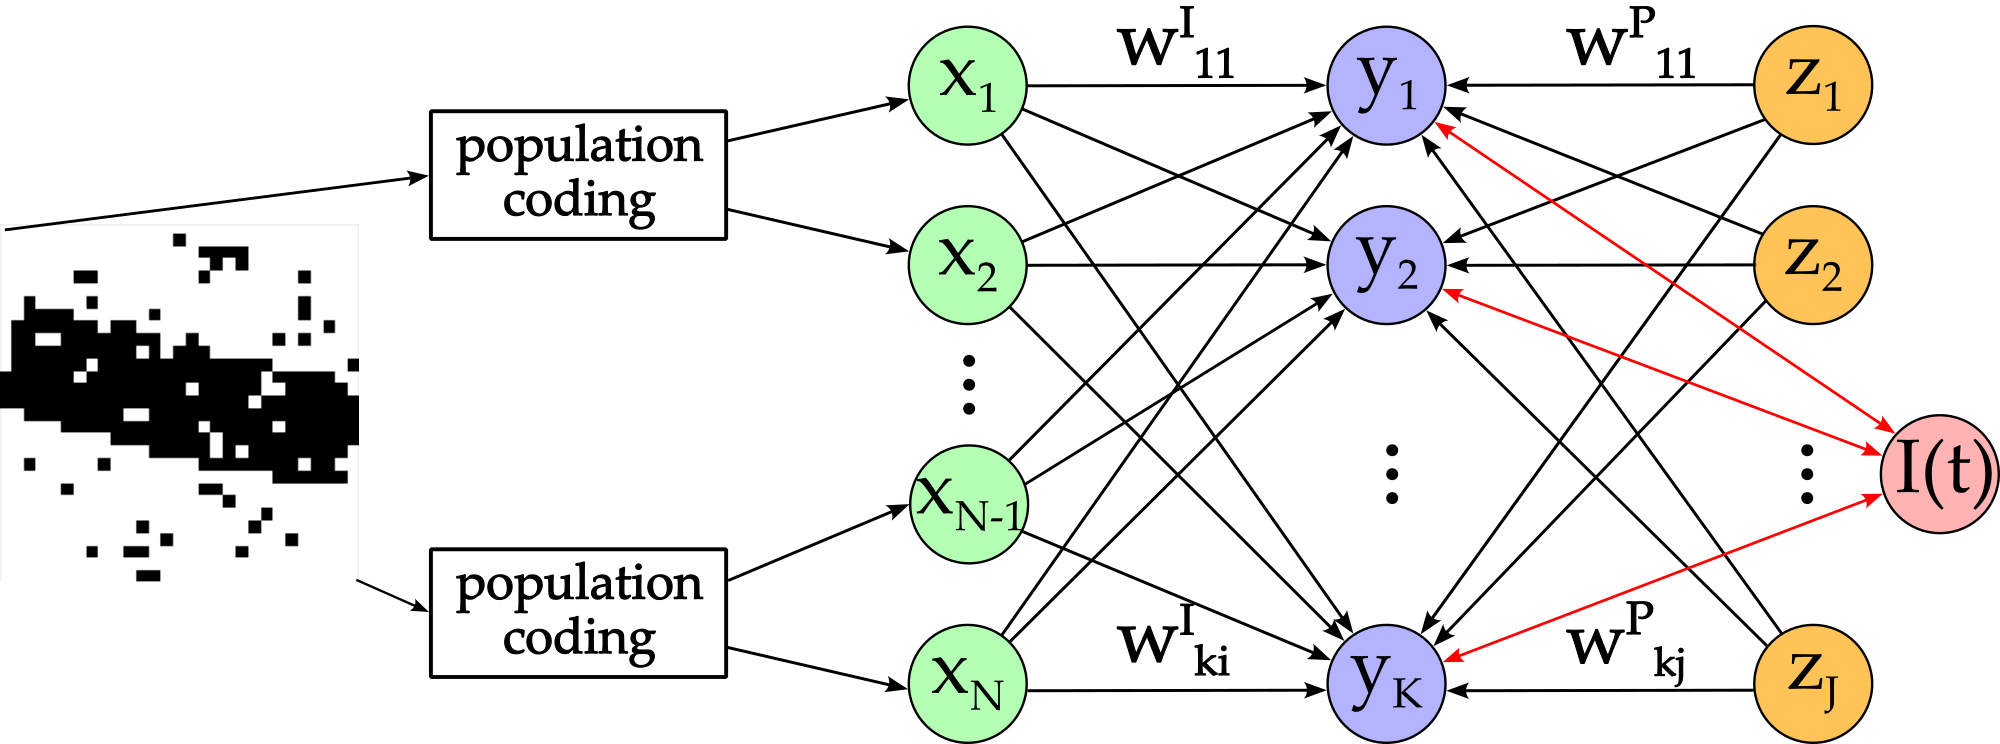
\includegraphics[width=\linewidth]{figures/networkPlan.png}
  \caption{Architecture of the network.}
\end{figure}

\paragraph{Neuron model}
As in \citet{nessler} the input neurons $x_1,...,x_N$ are firing according to a poisson process with an average firing rate $f_{input}$ when active and with 0 Hz when in an inactive state. The input neurons receive binary input, which is either a black, or a white pixel of an image. Each spike an input neuron generates was modelled by a double exponential kernel. As the signal is zero before the spike is generated, a Heaviside step function $\theta$ was applied to it, to limit the kernel to time ranges after the spike occurred. The Heaviside step function is given by
\begin{equation}
\theta (s) = \begin{dcases*} 1 & if $s \geq 0$ \\
0 & if $s < 0 $ \end{dcases*},
\end{equation}
where $s$ represents a time difference between the current simulation time and the time at which a spike occurred.
Multiplying $\theta(s)$ with the double exponential kernel yields the kernel function 
\begin{equation}
\varepsilon (s) = \theta (s) \cdot e^{-(s + \delta t) / \tau_{decay}} - e^{-(s + \delta t) / \tau_{rise}}.
\end{equation}
The kernel function has a time constant for the rise of the signal $\tau_{rise} = 1\text{ ms}$ and a time constant for the decay of the signal $\tau_{decay} = 15\text{ ms}$. The time step size of the simulation is $\delta t = 1\text{ ms}$. It had to be added to the double exponential kernel for numerical reasons, to evaluate the time at the end of the current simulation step, rather than at the beginning. A visualization of the kernel function can be seen in Figure \ref{fig:kernelFunction}. 

\begin{figure}
  \centering
  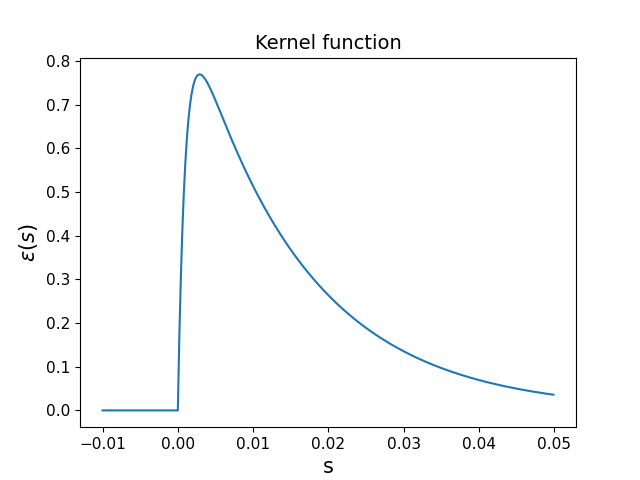
\includegraphics[width=0.6\linewidth]{figures/kernelFunction.png}
  \caption{Visualization of the kernel function $\varepsilon (s)$ within the relevant time window. A double exponential kernel was used. To limit the kernel function to positive values of s a Heaviside step function was applied. The output of this function was used to calculate the unweighed membrane potential response. }
  \label{fig:kernelFunction}
\end{figure}

Several input neuron spikes can happen in a short time window, increasing the unweighed membrane potential response $x_i(t)$. Depending on the timing of the spikes, they contribute additively to $x_i(t)$. The unweighed membrane potential response is given by

\begin{equation}
x_i(t) = \sum_{t_i^{(f)}} \varepsilon (t - t_i^{(f)}),
\end{equation}
with $t$ being the current simulation time and $t_i^{(f)}$ the time at which the input spike occurred.
Analogously, the unweighed membrane potential response of the prior neurons is given by
\begin{equation}
z_j(t) = \sum_{t_p^{(f)}} \varepsilon (t - t_p^{(f)}).
\end{equation}
 
The membrane potential $u_k$ of each output neuron is calculated by multiplying the unweighed membrane potential response of each input neuron times the input weight $w^{I}_{ki}$ of the connection between them, plus the unweighed membrane potential response of each prior neuron times the prior weight $w^{P}_{kj}$
\begin{equation}
\label{eqn:uk}
u_k(t) = \sum_{i=1}^N w^{I}_{ki} \cdot x_i(t) + \sum_{j=1}^J w^{P}_{kj} \cdot z_j(t).
\end{equation}
In \citet{nessler} each output neuron $y_k$ also had an intrinsic excitability $w_{k0}$, which was learned for each neuron. For the experiments of this thesis it was omitted, as the different classes of  input images were equally likely, thus the intrinsic excitabilities of the output neurons would all end up being equal to each other.

\citet{nessler} defined that the firing probability of an output neuron  $y_k$ is exponentially proportional to its membrane potential $u_k$ minus the received inhibition $I(t)$
\begin{equation}
\label{eqn:pVonY}
p(y_k \text{ fires at time t}) \propto e^{u_k(t) - I(t)}.
\end{equation}
This stochastic firing model is supported by experimental biological evidence \citep{woDasEHerkommt}. Through this definition the firing rate $r_k(t)$ of an output neuron is then modelled by an inhomogeneous Poisson process as
\begin{equation}
\label{eqn:rk}
r_k(t) = e^{u_k(t) - I(t)}.
\end{equation}
At every timestep of the simulation the inhibition signal $I(t)$ is subtracted from the membrane potential $u_k(t)$ of every output neuron. By that, the membrane potentials are altered to always yield a spiking frequency of 200 Hz, regardless if it would be lower or higher without it. This means that the adaptive inhibition signal can also function as an excitatory signal. 

The total firing rate of the output neurons $R(t)$	 is obtained by summing up the firing rates of all output neurons, yielding 
\begin{equation}
\label{eqn:R}
R(t) = \sum_{k=1}^K e^{u_k(t) - I(t)}.
\end{equation}

The inhibition signal $I(t)$ was chosen to depend on the current membrane potential of the output neurons. 
Solving Equation \ref{eqn:R} for $I(t)$ yields
\begin{equation}
\label{}
R(t) = \frac{ \sum_{k=1}^K e^{u_k(t)}}{e^{I(t)}}
\end{equation}
\begin{equation}
\label{}
e^{I(t)} = \frac{\sum_{k=1}^K e^{u_k(t)}}{R(t)}
\end{equation}
\begin{equation}
\label{}
I(t) = \ln{ \frac{ \sum_{k=1}^K e^{u_k(t)}}{R(t)}}
\end{equation}
\begin{equation}
\label{eqn:I(t)}
I(t) =  - \ln{R(t)} + \ln{  \sum_{k=1}^K e^{u_k(t)}}.
\end{equation}

The probability of an individual output neuron to fire within a time step $\delta t$ is given by
\begin{equation}
\label{eqn:rkdt}
r_k(t) \delta t.
\end{equation}

The conditional probability $q_k(t)$ that a spike originated from the output neuron $y_k$ is given by
\begin{equation}
\label{eqn:qk}
q_k(t) = \frac{r_k(t) \delta t}{R(t) \delta t} = \frac{e^{u_k(t) - I(t)}}{\sum_{k'=1}^K e^{u_{k'}(t) - I(t)}} = \frac{e^{u_k(t)}}{\sum_{k'=1}^K e^{u_{k'}(t)}}.
\end{equation}
The inhibition term cancels out because all output neurons receive the same inhibition, meaning that it is independent of k. Whenever an output spike should be generated within a time step, according to Equation \ref{eqn:rkdt}, it is determined via the discrete probability distribution $q_k(t)$ from which $y_k$ the spike originates. As $R(t)$ has a fixed value of 200 Hz, which is ensured by $I(t)$, it is unlikely that another output spike is generated shortly after the first one. This means, that the output spike generation functions as a soft-WTA function.
 
\paragraph{Spike timing dependent plasticity}
The input weights $w^{I}_{ki}$ between neurons $x_i$ and $y_k$ are updated whenever an output neuron fires. $\sigma$ determines the time window, after which spikes are no longer considered. If $y_k$ produces a spike, all its weights to the input neurons are updated as
\begin{equation}
\label{deltawki}
\Delta w^{I}_{ki} = \begin{dcases*} \lambda \cdot (ce^{-w^{I}_{ki}} - 1) & if $x_{i}$ fired in $ [t^f - \sigma, t^f] $ \\
\lambda \cdot (-1) & \text{if $ x_i $ did not fire in $ [t^f - \sigma, t^f] $, } \end{dcases*}
\end{equation}
where $\lambda$ is the learning rate, the hyperparameter c shifts the weight values, $t^f$ is the time when $y_k$ spiked and $\sigma$ is the time window in which input spikes are considered as "before" an output spike. As the membrane potentials $u_k$ of the output neurons result from the addition of the EPSPs of the input neurons times the corresponding weight, a way to control the average size of $u$ is needed. If $u$ is too small, the output neurons will fire too sparsely and if $u$ is too big, it will impair the learning process. So to limit $u$, the size of the weights is controlled via the hyperparameter c. The learning rate $\lambda$ is needed to control the size of each weight update. If it is too big, few output neurons will respond to too large parts of the input, while others might not respond at all. On the other hand if $\lambda$ is too small the network will learn very slowly and may never converge.
The prior weights $w^{P}_{kj}$ are also updated whenever an output neuron fires, in the same way as $w^{I}_{ki}$
\begin{equation}
\label{deltawkj}
\Delta w^{P}_{kj} = \begin{dcases*} \lambda \cdot (ce^{-w^{P}_{kj}} - 1) & if $z_{j}$ fired in $ [t^f - \sigma, t^f] $ \\
\lambda \cdot (-1) & \text{if $ z_j $ did not fire in $ [t^f - \sigma, t^f] $. } \end{dcases*}
\end{equation}

\section{Mathematical link between the spiking Winner-Take-All network model and Bayesian inference}
\label{linkNetworkBayes}

\citet{nessler} hypothesized that the ensemble of weights of a neuron can be understood as a generative model. They further claimed, that every synaptic weight, due to STDP-induced changes,  converges stochastically to the log of the conditional probability that the presynaptic neuron has fired just before the postsynaptic neuron, given that the postsynaptic neuron fires. This connection is given by
\begin{equation}
\label{eqn:weightProbLink}
 w^{I}_{ki} = log(p(x_i = 1 | Y = k))
\end{equation}
and will be analysed in Section \ref{section:1D}.
Furthermore, they claimed that in a Bayesian inference context, every input spike provides evidence for an observed variable and every output spike represents one stochastic sample from the posterior distribution over hidden causes, which are encoded in the circuit. 

%TODO WIP: abschreiben von Legi

1. Modellannahme
%TODO "i" bei prod und summer richtigstellen (bis N oder so...)
%TODO u^X_k usw... zuerst X
%TODO Legi mag X = \underline{x}  .... symbolisiert vector... vielleicht überall anpassen, oder ignorieren?
%TODO Legi sagt mein Bayes 3.3 anders argumentieren... machen...
%auch Z=j durch Z ersetzen auf der linken seite von equations...
\begin{equation}
\begin{split}
P(X=x|Y=k) &= \prod_i P(x_i=1|Y=k)^{x_i} \cdot P(x_i=0|Y=k)^{1-x_i}\\
log P(X=x|Y=k) &= \sum_i (x_i log P(x_i=1|Y=k) + (1-x_i) log (1 - P(x_i=1|Y=k)))
\end{split}
\end{equation}
With Equation \ref{eqn:weightProbLink}
\begin{equation}
P(X=x|Y=k) = \sum_i (x_i w_{ki} + (1-x_i)\overline{w_{ki}}) = u^X_k
\end{equation}
\begin{equation}
\Rightarrow P(X=x|Y=k) = e^{u^X_k}
\end{equation}

2. Modellannahme

\begin{equation}
\begin{split}
P(Y=k|Z) &= \prod_j P(Y=k|Z=j)^{z_j}\\
log P(Y=k|Z) &= \sum_j (z_j log P(Y=k|Z=j))
\end{split}
\end{equation}
With Equation \ref{eqn:weightProbLink}
\begin{equation}
P(Y=k|Z) = \sum_j (z_j w^P_{kj}) = u^Z_k
\end{equation}
\begin{equation}
\Rightarrow P(Y=k|Z) = e^{u^Z_k}
\end{equation}

Die 2 einsetzen in Equation \ref{eqn:pYvorausgesetztXUndZ}

\begin{equation}
\begin{split}
P(Y=k|X=x,Z) &= \frac{e^{u^X_k} e^{u^Z_k}}{\sum_{k'} e^{u^X_{k'}} e^{u^Z_{k'}}}\\
&= \frac{e^{u^X_k + u^Z_k}}{\sum_{k'} e^{u^X_{k'} + u^Z_{k'}}}
\end{split}
\end{equation}
and this shows why for uk the 2 terms were added.

%TODO Das danach wegschmeißen... werd neues
%darüber einfügen
To explain the connection between the spiking Winner-Take-All network model and Bayesian inference it will be demonstrated, that the posterior probability of Bayesian inference given in Equation \ref{eqn:pYvorausgesetztXUndZ} is equal to the relative firing probability $q_k(t)$, given in Equation \ref{eqn:qk}.

As explained in Section \ref{section:bayesianInference}, the visual input, modelled by the input neurons, can be thought of as the Bayesian likelihood $P(X|Y)$ and the feedback, modelled by the prior neurons, as the Bayesian prior $P(Y|Z)$.

It is argued that $P(X=x|Y=k)$ equals $q_k^X(t)$. $q_k^X(t)$ is the conditional probability of an output neuron $Y_k$ for the given input vector $X=x$. It can be calculated similarly to $q_k(t)$, but without the contribution of the prior neurons. Thus, the partial membrane potential, caused by the input neurons, is needed and given by 
\begin{equation}
u_k^X(t) = \sum_{i=1}^N w^{I}_{ki} \cdot x_i(t).
\end{equation}
Inserting $u_k^X(t)$, instead of $u_k(t)$ into Equation \ref{eqn:qk} yields
\begin{equation}
q_k^X(t) = \frac{e^{u_k^X(t)}}{\sum_{k'=1}^K e^{u_{k'}^X(t)}} = P(X=x|Y=k).
\end{equation}

Similarly, it is argued that $P(Y=k|Z=j)$ equals $q_k^Z(t)$. $q_k^Z(t)$ is the conditional probability of an output neuron $y_k$, given the activity of a prior neuron $z_j$.  
Analogously to $u_k^X(t)$, the partial membrane potential, caused by the prior neurons, is given by
\begin{equation}
u_k^Z(t) = \sum_{j=1}^J w^{P}_{kj} \cdot z_j(t).
\end{equation}
Inserting $u_k^Z(t)$, instead of $u_k(t)$, into Equation\ref{eqn:qk} yields
\begin{equation}
q_k^Z(t) = \frac{e^{u_k^Z(t)}}{\sum_{k'=1}^K e^{u_{k'}^Z(t)}} = P(Y=k|Z=j).
\end{equation}

When inserting the likelihood and the prior into Equation \ref{eqn:pYvorausgesetztXUndZ} we get
\begin{equation}
\label{eqn:posteriorFull}
\begin{split}
P(Y=k|X=x,Z=j) &= \frac{e^{u_k^X(t)} \cdot e^{u_k^Z(t)} }{\sum_{k'=1}^K  e^{u_{k'}^X(t)} \cdot e^{u_{k'}^Z(t)}} \\
&= \frac{e^{\sum_{i=1}^N w^{I}_{ki} \cdot x_i(t)} \cdot e^{\sum_{j=1}^J w^{P}_{kj} \cdot z_j(t)} }{\sum_{k'=1}^K  e^{\sum_{i=1}^N w^{I}_{k'i} \cdot x_i(t)} \cdot e^{\sum_{j=1}^J w^{P}_{k'j} \cdot z_j(t)}} \\
&= \frac{e^{\sum_{i=1}^N w^{I}_{ki} \cdot x_i(t) + \sum_{j=1}^J w^{P}_{kj} \cdot z_j(t) }}{\sum_{k'=1}^K  e^{\sum_{i=1}^N w^{I}_{k'i} \cdot x_i(t) + \sum_{j=1}^J w^{P}_{k'j} \cdot z_j(t)}}
\end{split}
\end{equation}

According to Equation \ref{eqn:qk} and \ref{eqn:uk}
\begin{equation}
\label{eqn:qpExpanded}
\begin{split}
q_k(t) &= \frac{e^{u_k(t)}}{\sum_{k'=1}^K e^{u_{k'}(t)}} \\
&= \frac{e^{\sum_{i=1}^N w^{I}_{ki} \cdot x_i(t) + \sum_{j=1}^J w^{P}_{kj} \cdot z_j(t)}}{\sum_{k'=1}^K e^{\sum_{i=1}^N w^{I}_{k'i} \cdot x_i(t) + \sum_{j=1}^J w^{P}_{k'j} \cdot z_j(t)}}.
\end{split}
\end{equation}

From Equations \ref{eqn:posteriorFull} and \ref{eqn:qpExpanded} we can conclude that
\begin{equation}
P(Y=k|X=x,Z=j) = q_k(t).
\end{equation}
This showed, that the Bayesian posterior is equal to the conditional probability $q_k(t)$. Furthermore, it showed that the extension of $u_k(t)$, in Equation \ref{eqn:uk}, with the prior term was correct.

\chapter{Experiments}
% \section{Experiment 1: Rotated Bars}
\label{section:rotatedLines}
\subsection{Introduction}
The goal of this task was to recreate example 2 from \citet{nessler}. In this example they fed a winner-take-all spiking neural network images with bars in different orientations on them. The network then clustered the images into ten groups depending on their orientation.

\subsection{Methods}
\paragraph{Input data}
The images used in this task were generated with a size of 29 x 29 pixels. Black bars with a width of 7 pixels going through the center of the image were drawn onto a white background. To simulate noise each pixel had a chance of ten percent to have its color flipped. To ensure that all bars in the images have the same length regardless of their orientation a circular mask with a radius of 15 pixels was applied to the images. This recolored all pixels outside of the mask to white. During the training of the network one image per iteration was generated in a uniformly distributed orientation and each image was shown for 200 ms. For the training of the network 4000 of these images were shown. The randomly chosen orientation could lie between 0 and 359 degrees.  Two examples of such images can be seen in Figure \ref{fig:angleImages}.

\begin{figure}
  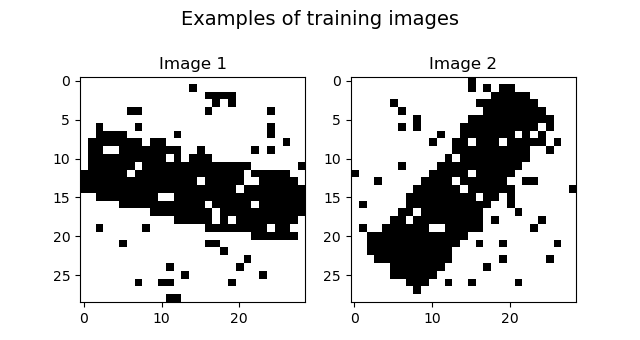
\includegraphics[width=\linewidth]{figures/angleNetwork/trainingImages.png}
  \caption{Two examples of the generated training data in this experiment.}
  \label{fig:angleImages}
\end{figure}

\paragraph{Neuron model}

As in \citet{nessler} the input neurons X are firing according to a poisson process with an average firing rate of 20 Hz when active and with 0 Hz when in an inactive state. The excitatory post synaptic potentials (EPSPs) $x_i(t)$ that these neurons produce can be seen in Figure \ref{fig:XSpike}. A double exponential kernel was used to generate the EPSP. The time constant for the rise of the signal $\tau_{rise}$ was 1 ms and the time constant for the decay of the signal $\tau_{decay}$ was 15 ms. The addition of the time step size $\delta t$ was necessary to get the time t at the end of the current simulation step. $t_f$ is the time at which the spike of $x_i$ occurred
\begin{equation}
\label{eqn:EPSP}
x_i(t) = e^{-(t + \delta t - t_f) / \tau_{decay}} - e^{-(t + \delta t - t_f) / \tau_{rise}}.
\end{equation}


\begin{figure}
  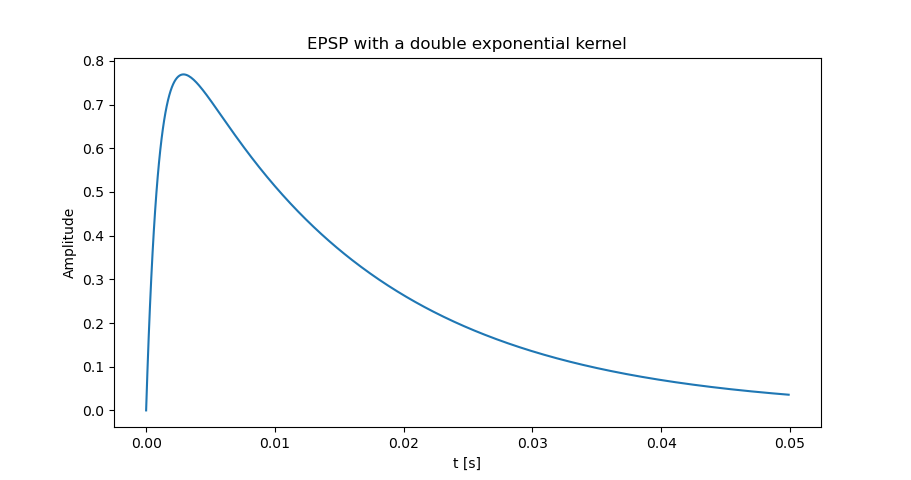
\includegraphics[width=\linewidth]{figures/XSpike.png}
  \caption{Form of an excitatory post synaptic potential generated by an input neuron over time. A double exponential kernel was used to generate this signal. These signals are fed to the next layer of the network. }
  \label{fig:XSpike}
\end{figure}

The firing rate of an output neuron $y_k$ is given by
\begin{equation}
\label{eqn:rk}
r_k(t) = e^{u_k(t) - I(t)}.
\end{equation}
The probability of an individual output neuron to fire within a time step $\delta t$ is given by
\begin{equation}
\label{eqn:rkdt}
r_k(t) \cdot \delta t.
\end{equation}

\paragraph{Network architecture}
Each pixel of an input image was connected to two neurons. The first of these neurons is in an active state when the pixel is black and in an inactive state otherwise. The second neuron expresses the opposite behaviour. As a consequence the network needs 1682 ($29 \cdot 29 \cdot 2$) excitatory input neurons $x_1,...,x_n$. These input neurons are fully connected to ten excitatory output neurons $y_1,...,y_k$. This means that that every input neuron $x_i$ is connected to each output neuron $y_k$. The membrane potential $u_k$ of each output neuron is calculated by multiplying the EPSP of each input neuron times the weight of the connection between them
\begin{equation}
\label{eqn:uk}
u_k(t) = \sum_{i=1}^n w_{ki} \cdot x_i(t).
\end{equation}
In \citet{nessler} each output neuron $y_k$ also had an intrinsic excitability $w_{k0}$ which was learned for each neuron. For this experiment however it was omitted, as each orientation of input images was equally likely, thus the intrinsic excitability of each output neuron would end up being the same.

The output neurons are modelled in a winner-takes-all (WTA) circuit. This means that whenever one output neuron spikes, a lateral inhibitory signal is fed to all output neurons, thus preventing the further activation of them for $\sigma_{inh} = 5 ms$. After completion of the training of the network each output neuron should be active for bars in a coherent area. Each of those areas should ideally be of equal size. As the bars can be oriented between 0 and 359 degrees, but each 180 degree rotation of an image results in an equivalent image, the desired size of the active area of an output neuron should be 18 degrees.


\paragraph{Inhibition}
The inhibition signal was chosen to depend on the current membrane potential of the output neurons. According to \citet{nessler} the total firing rate of the output neurons is
\begin{equation}
\label{eqn:R}
R(t) = \sum_{k=1}^K e^{u_k(t) - I(t)}.
\end{equation}
Solving this equation for I(t) yields
\begin{equation}
\label{}
R(t) = \frac{ \sum_{k=1}^K e^{u_k(t)}}{e^{I(t)}}
\end{equation}
\begin{equation}
\label{}
e^{I(t)} = \frac{\sum_{k=1}^K e^{u_k(t)}}{R(t)}
\end{equation}
\begin{equation}
\label{}
I(t) = \ln{ \frac{ \sum_{k=1}^K e^{u_k(t)}}{R(t)}}
\end{equation}
\begin{equation}
\label{eqn:I(t)}
I(t) =  - \ln{R(t)} + \ln{  \sum_{k=1}^K e^{u_k(t)}}.
\end{equation}
When implementing the inhibition the $- \ln{R(t)}$ term of Equation \ref{eqn:I(t)} was overlooked, that means it was assumed to be zero. Because of that R(t) equals 1 when the inhibition is active. This error was not detected at first, as the chance that a Y neuron fires within a time step of 1 ms with active inhibition is 1/1000 due to that oversight.

Whenever an output neuron produces a spike the inhibition signal I(t) is subtracted from the membrane potential $u_k(t)$ of every output neuron. This happens for the duration of $\sigma_{inh} = 5 ms$. Thus follows

\begin{equation}
\label{eqn:iinh}
I(t) = \begin{dcases*} \ln ( \sum_{i=1}^k e^{u_k} ) & if any $y_k$ fired in $ [t^f, t^f  + \sigma_{inh}] $ \\
0 & \text{if any $y_k$ did not fire in $ [t^f, t^f + \sigma_{inh}] $. } \end{dcases*}\end{equation}

\paragraph{Spike timing dependent plasticity}
!!!!! STDP WAS ALREADY EXPLAINED IN THEORETICAL BACKGROUND. THUS ENSURE THAT NOTHING HERE IS EXPLAINED AGAIN!!!!
The weights $w_{ki}$ between neurons $x_i$ and $y_k$ are updated whenever an output neuron fires. The time window $\sigma$ was set to 10 ms according to \citet{nessler}. If $y_k$ produces a spike all its weights are updated as
\begin{equation}
\label{deltawki}
\Delta w_{ki} = \begin{dcases*} \lambda \cdot (ce^{-w_{ki}} - 1) & if $x_{i}$ fired in $ [t^f - \sigma, t^f] $ \\
\lambda \cdot (-1) & \text{if $ x_i $ did not fire in $ [t^f - \sigma, t^f] $, } \end{dcases*}
\end{equation}
where $\lambda$ is the learning rate, the parameter c shifts the weight values, $t^f$ is the time when $y_k$ spiked and $\sigma$ is the time window in which input spikes are considered as "before" an output spike. As the membrane potentials $u_k$ of the output neurons result from the addition of the EPSPs of the 1682 input neurons times the corresponding weight, a way to control the average size of u is needed. If u is to small the output neurons will fire too sparsely and if u is too big it will impair the learning process. So to limit u, the size of the weights is controlled via the parameter c. The learning rate $\lambda$ is needed to control the size of each weight update. If it is too big few output neurons will take over more than the expected 18° areas and others will only respond for smaller areas or not at all. On the other hand if $\lambda$ is too small the network will learn very slowly and may never converge. Due to these two parameters being unwieldy to determine analytically they were chosen via grid search. 


\subsection{Results}

\paragraph{Parameter search}
The two parameters c, which controls the size of the weights, and the learning rate $\lambda$ were fitted to the network via grid search.	The tested parameters were as follows:
\begin{itemize}
  \item $c = 1$ ($\lambda = 10^{-2}, 10^{-3}, 10^{-4}$) 
  \item $c = 10$ ($\lambda = 10^{-2}, 10^{-3}, 10^{-4}$) 
  \item $c = 20$ ($\lambda = 10^{-2}, 10^{-2.5}, 10^{-3}, 10^{-3.5},  10^{-4}, 10^{-4.5}, 10^{-5}$) 
  \item $c = 30$ ($\lambda = 10^{-2}, 10^{-2.5}, 10^{-3}, 10^{-3.5}$) 
\end{itemize}
The simulation was conducted by simulating small discrete time steps and calculating the changes of the network in each step. The step size $\delta t$ was chosen as 1 ms.

\paragraph{$c = 1$}
The best results for $c = 1$ were achieved with $\lambda = 10^{-2}$. But overall this value for c did not work, even tough the network did learn to cluster images into eight groups depending on their orientation. In Figure \ref{fig:c1Pie} one can see which output neuron was the most active during the training process for each angle in 1° steps.

\begin{figure}
  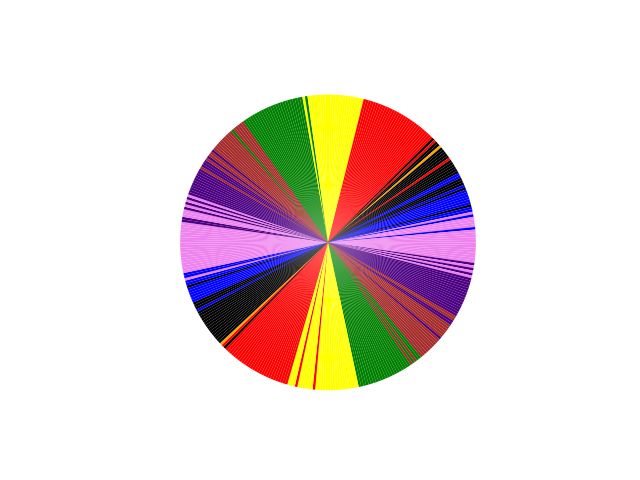
\includegraphics[width=\linewidth]{figures/angleNetwork/c1Pie.png}
  \caption{Most active output neuron depending on orientation of the training image during the training process. $c = 1, \lambda = 10^{-2}$}
  \label{fig:c1Pie}
\end{figure}

In Figure \ref{fig:c1Distinct} the training progress of the network can be seen. The figure shows the number of distinct output neurons active during the presentation of each training image shown. Due to the large learning rate, compared to other values of c,  the network learned quickly. However after iteration 70 there were images shown for which not a single output neuron spiked. This dying out of the networks activity is due to the parameter c being too small, which leads to too low membrane potentials.

\begin{figure}
  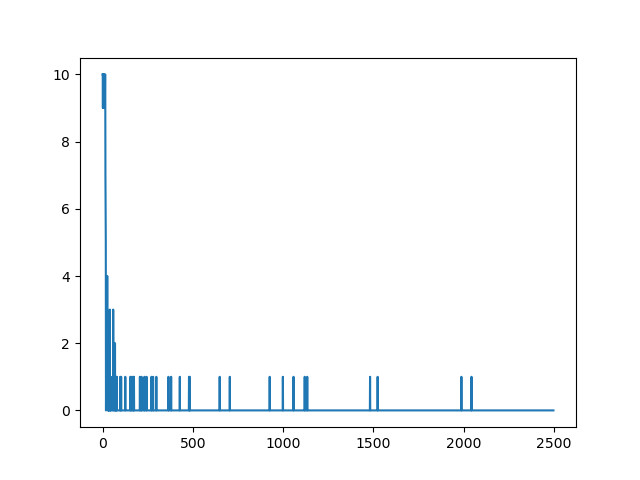
\includegraphics[width=\linewidth]{figures/angleNetwork/c1Distinct.png}
  \caption{Number of distinct output neurons active during the presentation duration of each training image. x-axis: image shown, y-axis: distinct output neurons active, $c = 1, \lambda = 10^{-2}$}
  \label{fig:c1Distinct}
\end{figure}

\paragraph{$c = 10$}
This value of $c = 10$ had the same problem of the network activity dying out as $c = 1$ although at a later point in time, as can be seen in Figure \ref{fig:c10Distinct}. Also in Figure \ref{fig:c10LastSpikes} the last 50 output spikes of the training process can be seen. As indicated by Figure \ref{fig:c10Distinct} the activity is sparse.

\begin{figure}
  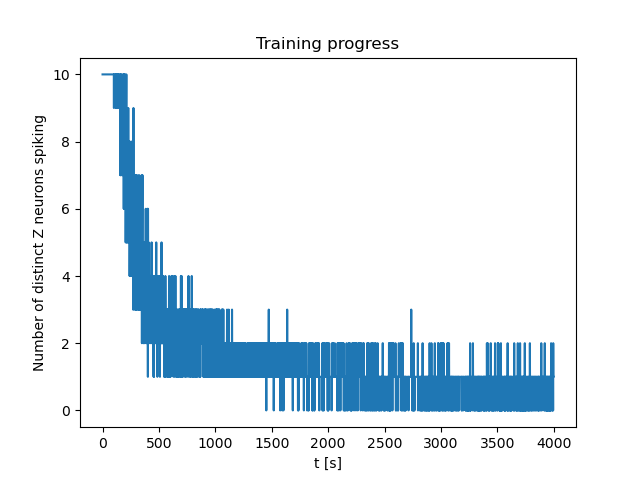
\includegraphics[width=\linewidth]{figures/angleNetwork/c10_3distinctZ.png}
  \caption{Number of distinct output neurons active during the presentation duration of each training image. x-axis: image shown, y-axis: distinct output neurons active, $c = 10, \lambda = 10^{-3}$}
  \label{fig:c10Distinct}
\end{figure}

\begin{figure}
  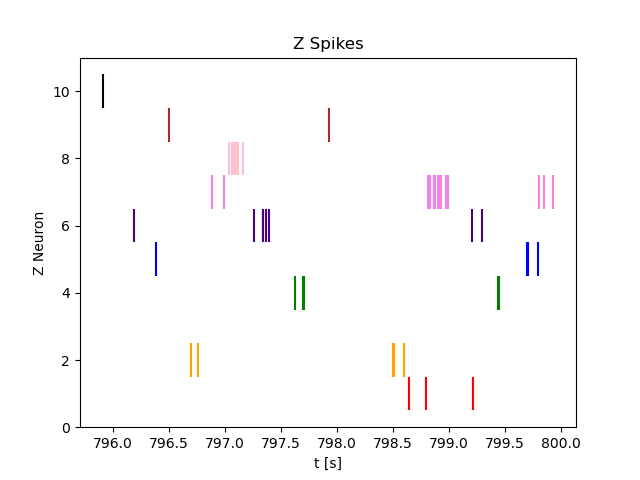
\includegraphics[width=\linewidth]{figures/angleNetwork/c10_3_50LastZSpikes.png}
  \caption{Last 50 output neuron spikes, $c = 10, \lambda = 10^{-3}$}
  \label{fig:c10LastSpikes}
\end{figure}

\paragraph{$c = 20$}
$c = 20$ was the first value for which the network activity did not die out after some time. For $\lambda = 10^{-2}$ one output neuron learned to spike first for every possible input image orientation, see Figure \ref{fig:c20_2Pie}. 

\begin{figure}
  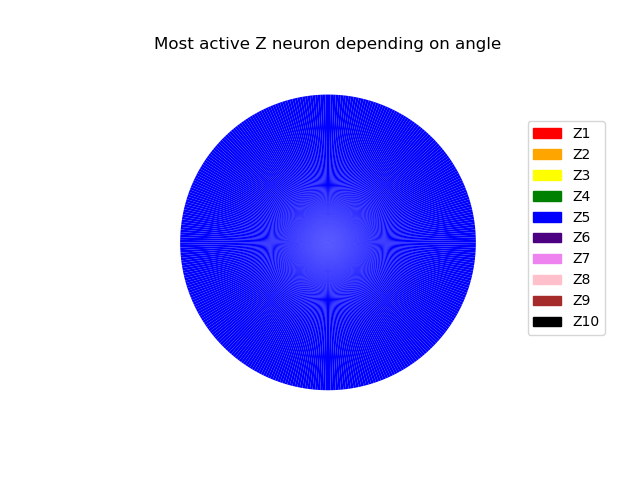
\includegraphics[width=\linewidth]{figures/angleNetwork/c20_2pie.png}
  \caption{Most active output neuron depending on orientation of the training image during the training process. $c = 20, \lambda = 10^{-2}$}
  \label{fig:c20_2Pie}
\end{figure}

With $c = 20$ and $\lambda = 10^{-3}$ the first combination that yielded a stable network was found. In Figure \ref{fig:c20_3Distinct} the amount of distinct output neurons firing during the presentation of each training image can be seen. Figure \ref{fig:c20_3averageZ} shows the proportion of the most active output neuron to all other output neurons active for each training image. Both of these figures can be used to measure the training progress of the network. Figure \ref{fig:c20_3averageZ} however shows the additional information how certain the network is that a training image belongs to a specific group.

\begin{figure}
  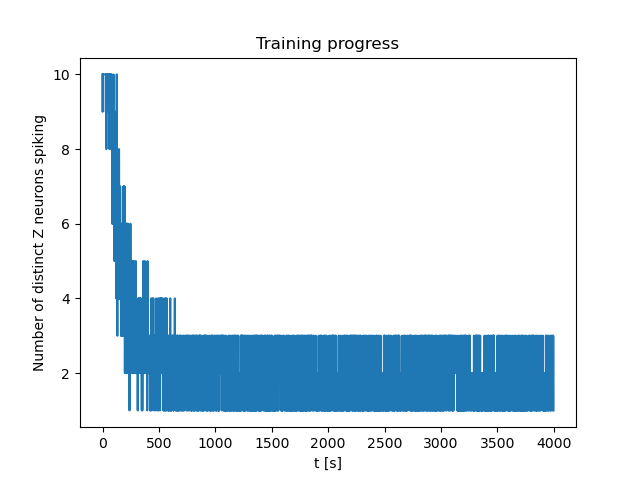
\includegraphics[width=\linewidth]{figures/angleNetwork/c20_3distinctZ.png}
  \caption{Number of distinct output neurons active during the presentation duration of each training image. x-axis: image shown, y-axis: distinct output neuron active, $c = 20, \lambda = 10^{-3}$}
  \label{fig:c20_3Distinct}
\end{figure}

\begin{figure}
  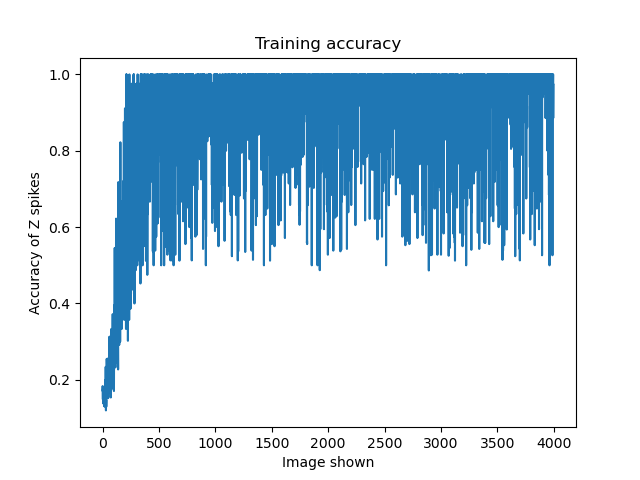
\includegraphics[width=\linewidth]{figures/angleNetwork/c20_3averageZ.png}
  \caption{Proportion (accuracy) of most active output neuron  to activity of all other output neurons during the presentation duration of each training image. $c = 20, \lambda = 10^{-3}$}
  \label{fig:c20_3averageZ}
\end{figure}

As this network did not die out after some time the trained network was analysed further. 180 images were generated in 1° steps and each was shown to the network for 200 ms. During each image presentation duration the most active output neuron was recorded. This yielded Figure \ref{fig:c20_3Pie}.

\begin{figure}
  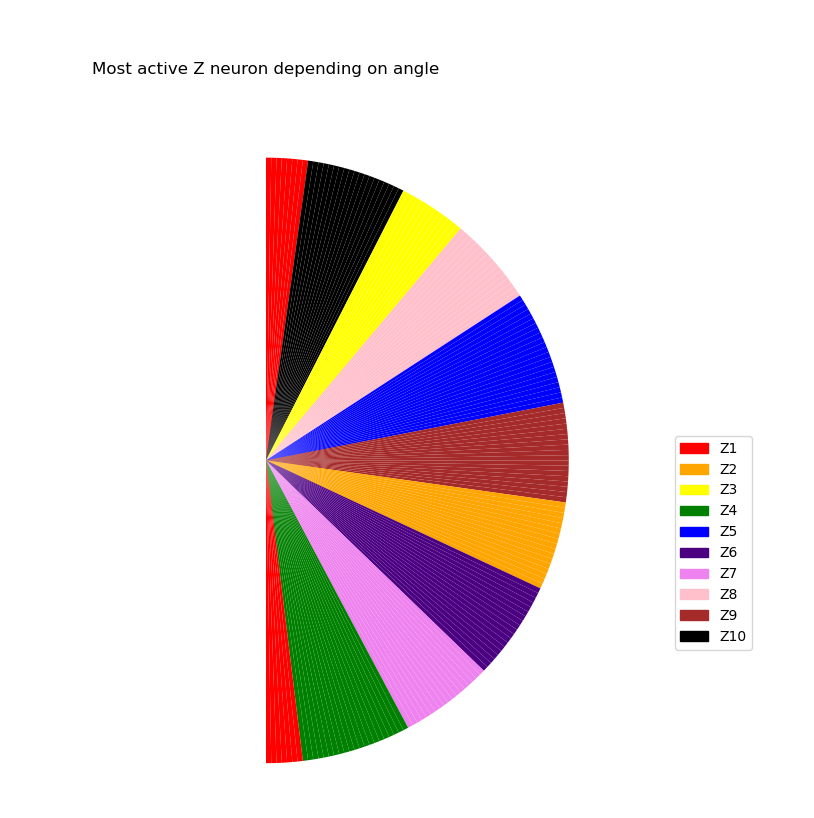
\includegraphics[width=\linewidth]{figures/angleNetwork/c20_3validationPie.png}
  \caption{Most active output neuron depending on orientation of the training image during the training process. $c = 20, \lambda = 10^{-3}$}
  \label{fig:c20_3Pie}
\end{figure}

Also the number of distinct output neurons firing during each image presentation was recorded and is shown in \ref{fig:c20_3validationDistinctZSpikes}. In this figure it seems that the points in which there are three distinct output neurons active are periodic in nature. This can be explained by Figure \ref{fig:c20_3validationZSpikes}. There it can be seen that whenever the image orientation nears the border between two competing output neurons both start to be active. This explains why for large parts of Figure \ref{fig:c20_3validationDistinctZSpikes} 2 neurons are active, as large portions of the bar in the image is overlapping the areas of the two nearest output neurons, thus producing high membrane potentials for both. The third distinct output neuron that is occasionally active seems to be of stochastic nature as much of the bars in the images overlaps areas of all other output neurons, thus generating a non zero membrane potential for each output neuron. However the occurrence of 3 distinct active output neurons seems to mostly occur at or close to the border between two competing output neurons, as there are already 2 distinct neurons firing by design.

\begin{figure}
  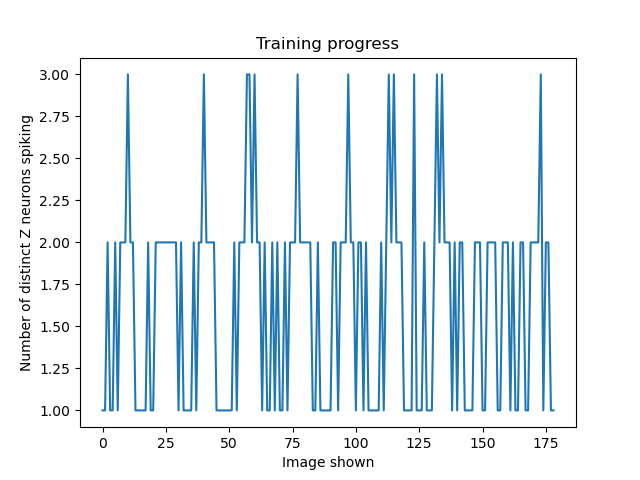
\includegraphics[width=\linewidth]{figures/angleNetwork/c20_3validationDistinctZSpikes.png}
  \caption{Number of distinct output neurons active during the presentation duration of each training image. x-axis: image shown, y-axis: distinct output neuron active, $c = 20, \lambda = 10^{-3}$}
  \label{fig:c20_3validationDistinctZSpikes}
\end{figure}

\begin{figure}
  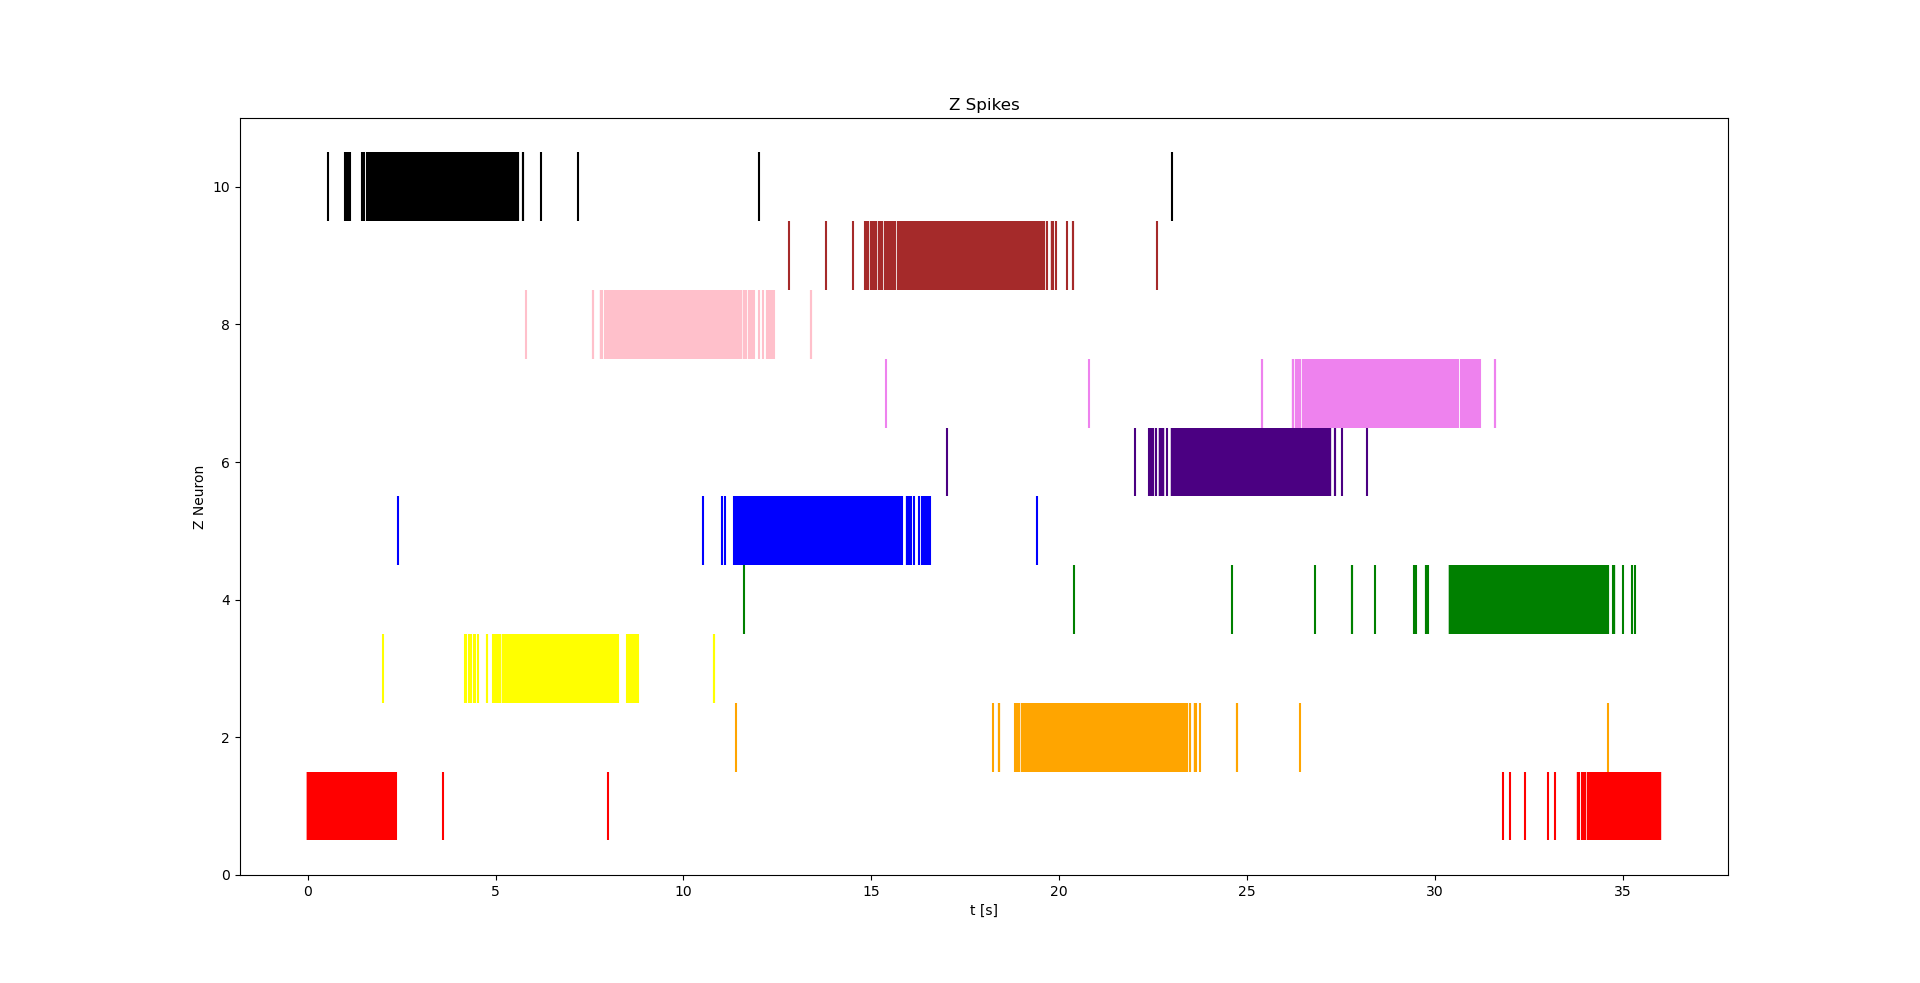
\includegraphics[width=\linewidth]{figures/angleNetwork/c20_3validationZSpikes.png}
  \caption{Output spikes over the presentation of input images from 0 to 179°, $c = 20, \lambda = 10^{-3}$}
  \label{fig:c20_3validationZSpikes}
\end{figure}

Also it was possible to project the learned weights $w_{ki}$ into the 2-D space to observe what they represent. This projection can be seen in Figure \ref{fig:c20_3weights2.png} for the weights of $y_{10}$.

\begin{figure}
  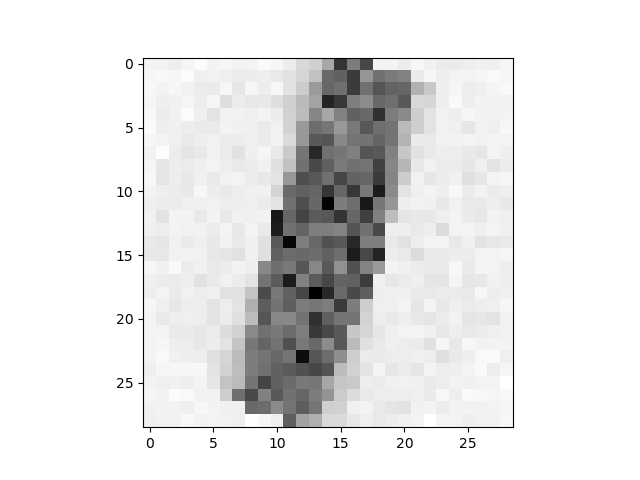
\includegraphics[width=\linewidth]{figures/angleNetwork/c20_3weights2.png}
  \caption{Visualization of the learned weights of $y_{10}$.}
  \label{fig:c20_3weights2.png}
\end{figure}

The results for smaller $\lambda$ were also valid, but they did not seem to yield superior results to the parameters $c = 20$ and $\lambda = 10^{-3}$. As with smaller learning rates the training simply took longer and the performance of the network did not improve they were discarded and  the learning rate $\lambda = 10^{-3}$ was declared winner for $c = 20$. To save space the figures of smaller learning rates will not be shown here.

\paragraph{$c = 30$}
also yielded a functioning network, but it did perform analogous to $c = 20$. It did perform in the same way, as with $c = 20$ the output neurons already fire every 5 ms, slowed down by the inhibition. By increasing c further the output neurons did not increase their activity.

\subsection{Conclusion}

The parameters $c = 20$ and $\lambda = 10^{-3} $ were finally chosen as the network performed the best and trained the quickest with these parameters, without raising the membrane potential needlessly.







\section{Experiment 3: Rotated bars with adaptive inhibition}
\label{section:rotatedLinesAdaptiveInhibition}

\subsection{Introduction}

This experiment analyses a different approach to the implementation of the inhibition of the output neurons. 
In Experiment \ref{section:rotatedLines} and \ref{section:horvert} the output neurons were stopped from firing for a defined time window after any output neuron fired. The time window during which the inhibition was active was 5 ms, which resulted in an average output firing rate of 200 Hz. In this experiment an adaptive inhibition will be used which will regulate the membrane potentials of the output neurons so that all of them together fire with 200 Hz on average. The distinction to the previous experiments is that there never is a time window in which no output neuron may fire. Also it is assumed that the weight shifting parameter c will not be needed to be fitted to the network, as the adaptive inhibition regulates the output firing rate of the network.

\subsection{Methods}

The adaptive inhibition is given by Equation \ref{eqn:I(t)} which was already used in Experiments \ref{section:rotatedLines} and \ref{section:horvert}. However the total output firing rate $R(t)$ was set to 200 Hz in this experiment.

\subsection{Results}

Several different values for the parameter c were tested. As expected the firing rate of the output neurons 200 Hz on average regardless of the value of c. However for values of c bigger than 100 the network did not learn correctly. For those values some output neurons learned to respond to areas of more than 18°, while other neurons did not respond to any areas. For $c = 20$ the network performed equally to Experiment \ref{section:rotatedLines}. The results for that parameter can be seen in Figures \ref{fig:angleNetworkAdaptiveInhibitionTraining}, \ref{fig:angleNetworkAdaptiveInhibitionOutputFiringRate} and \ref{fig:angleNetworkAdaptiveInhibitionValidation}.


\begin{figure}
  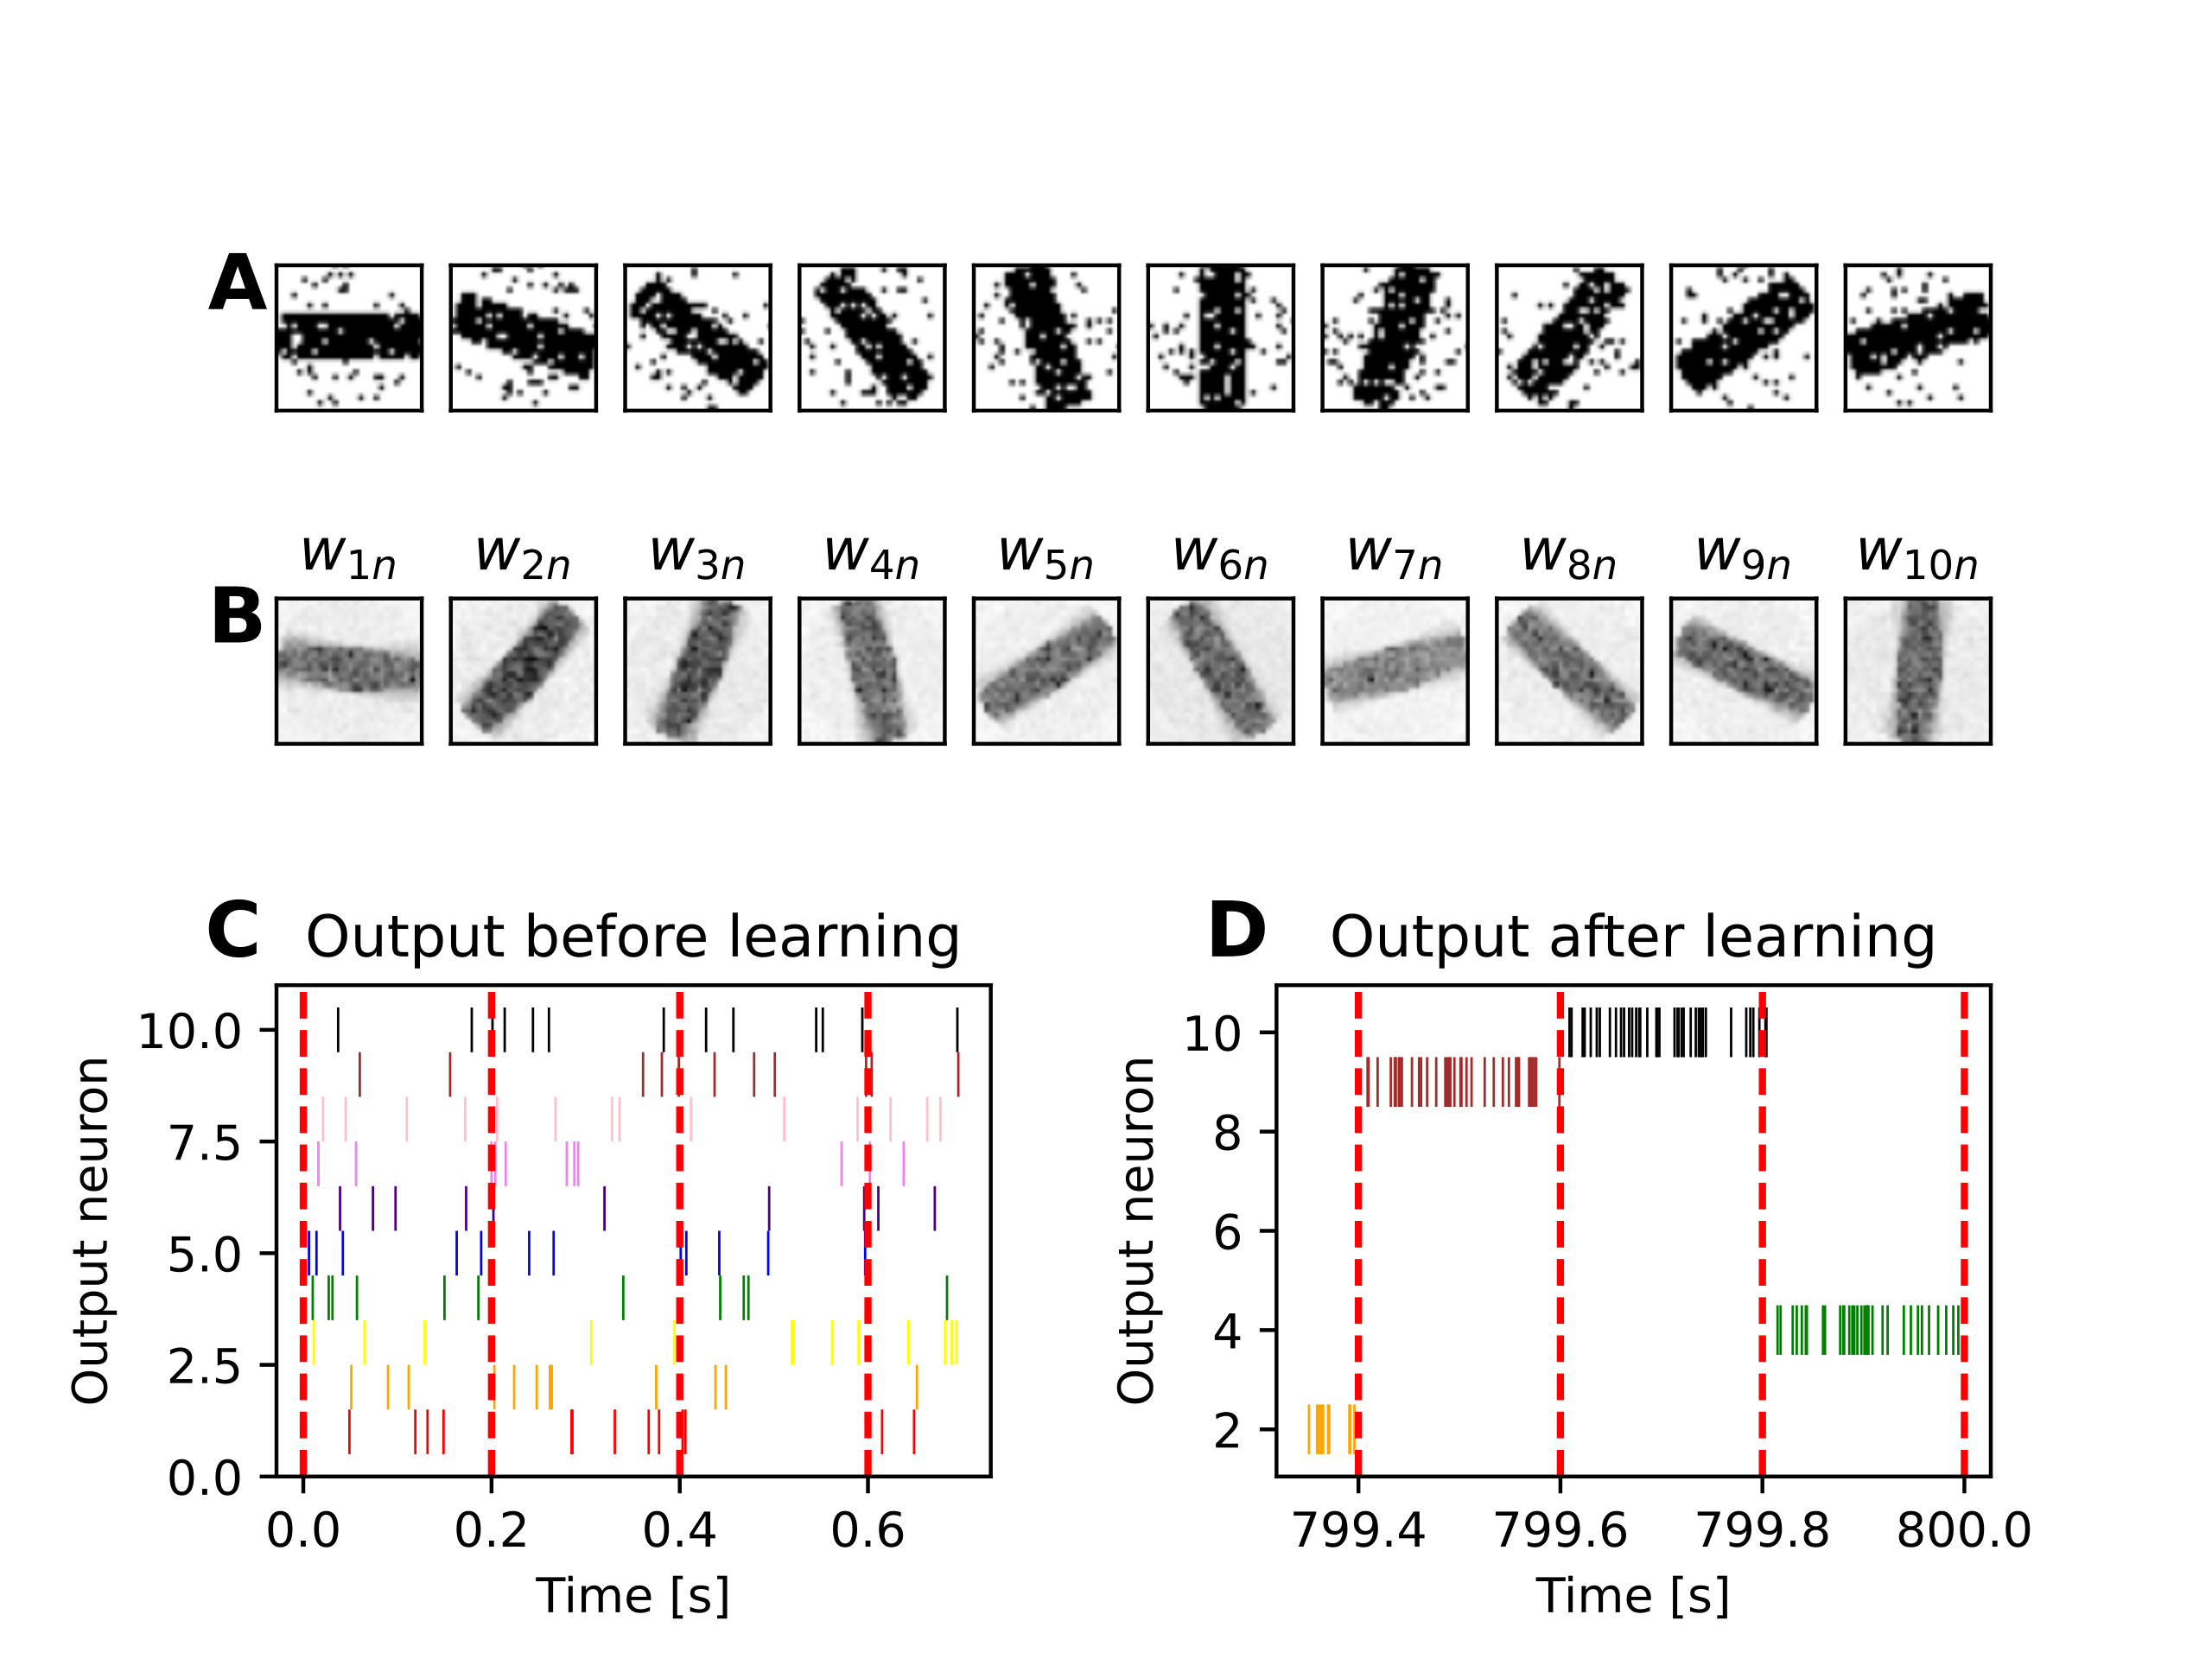
\includegraphics[width=\linewidth]{figures/angleAdaptiveInh/trainingPlot.png}
  \caption{\textbf{Training.} \textbf{A} Examples of 29 x 29-pixel input images of rotated bars and background noise. \textbf{B} Learned weights of the connections between input and output neurons. \textbf{C, D} Spike activity expressed by the output neurons before and after the training of the network. }
  \label{fig:angleNetworkAdaptiveInhibitionTraining}
\end{figure}

\begin{figure}
  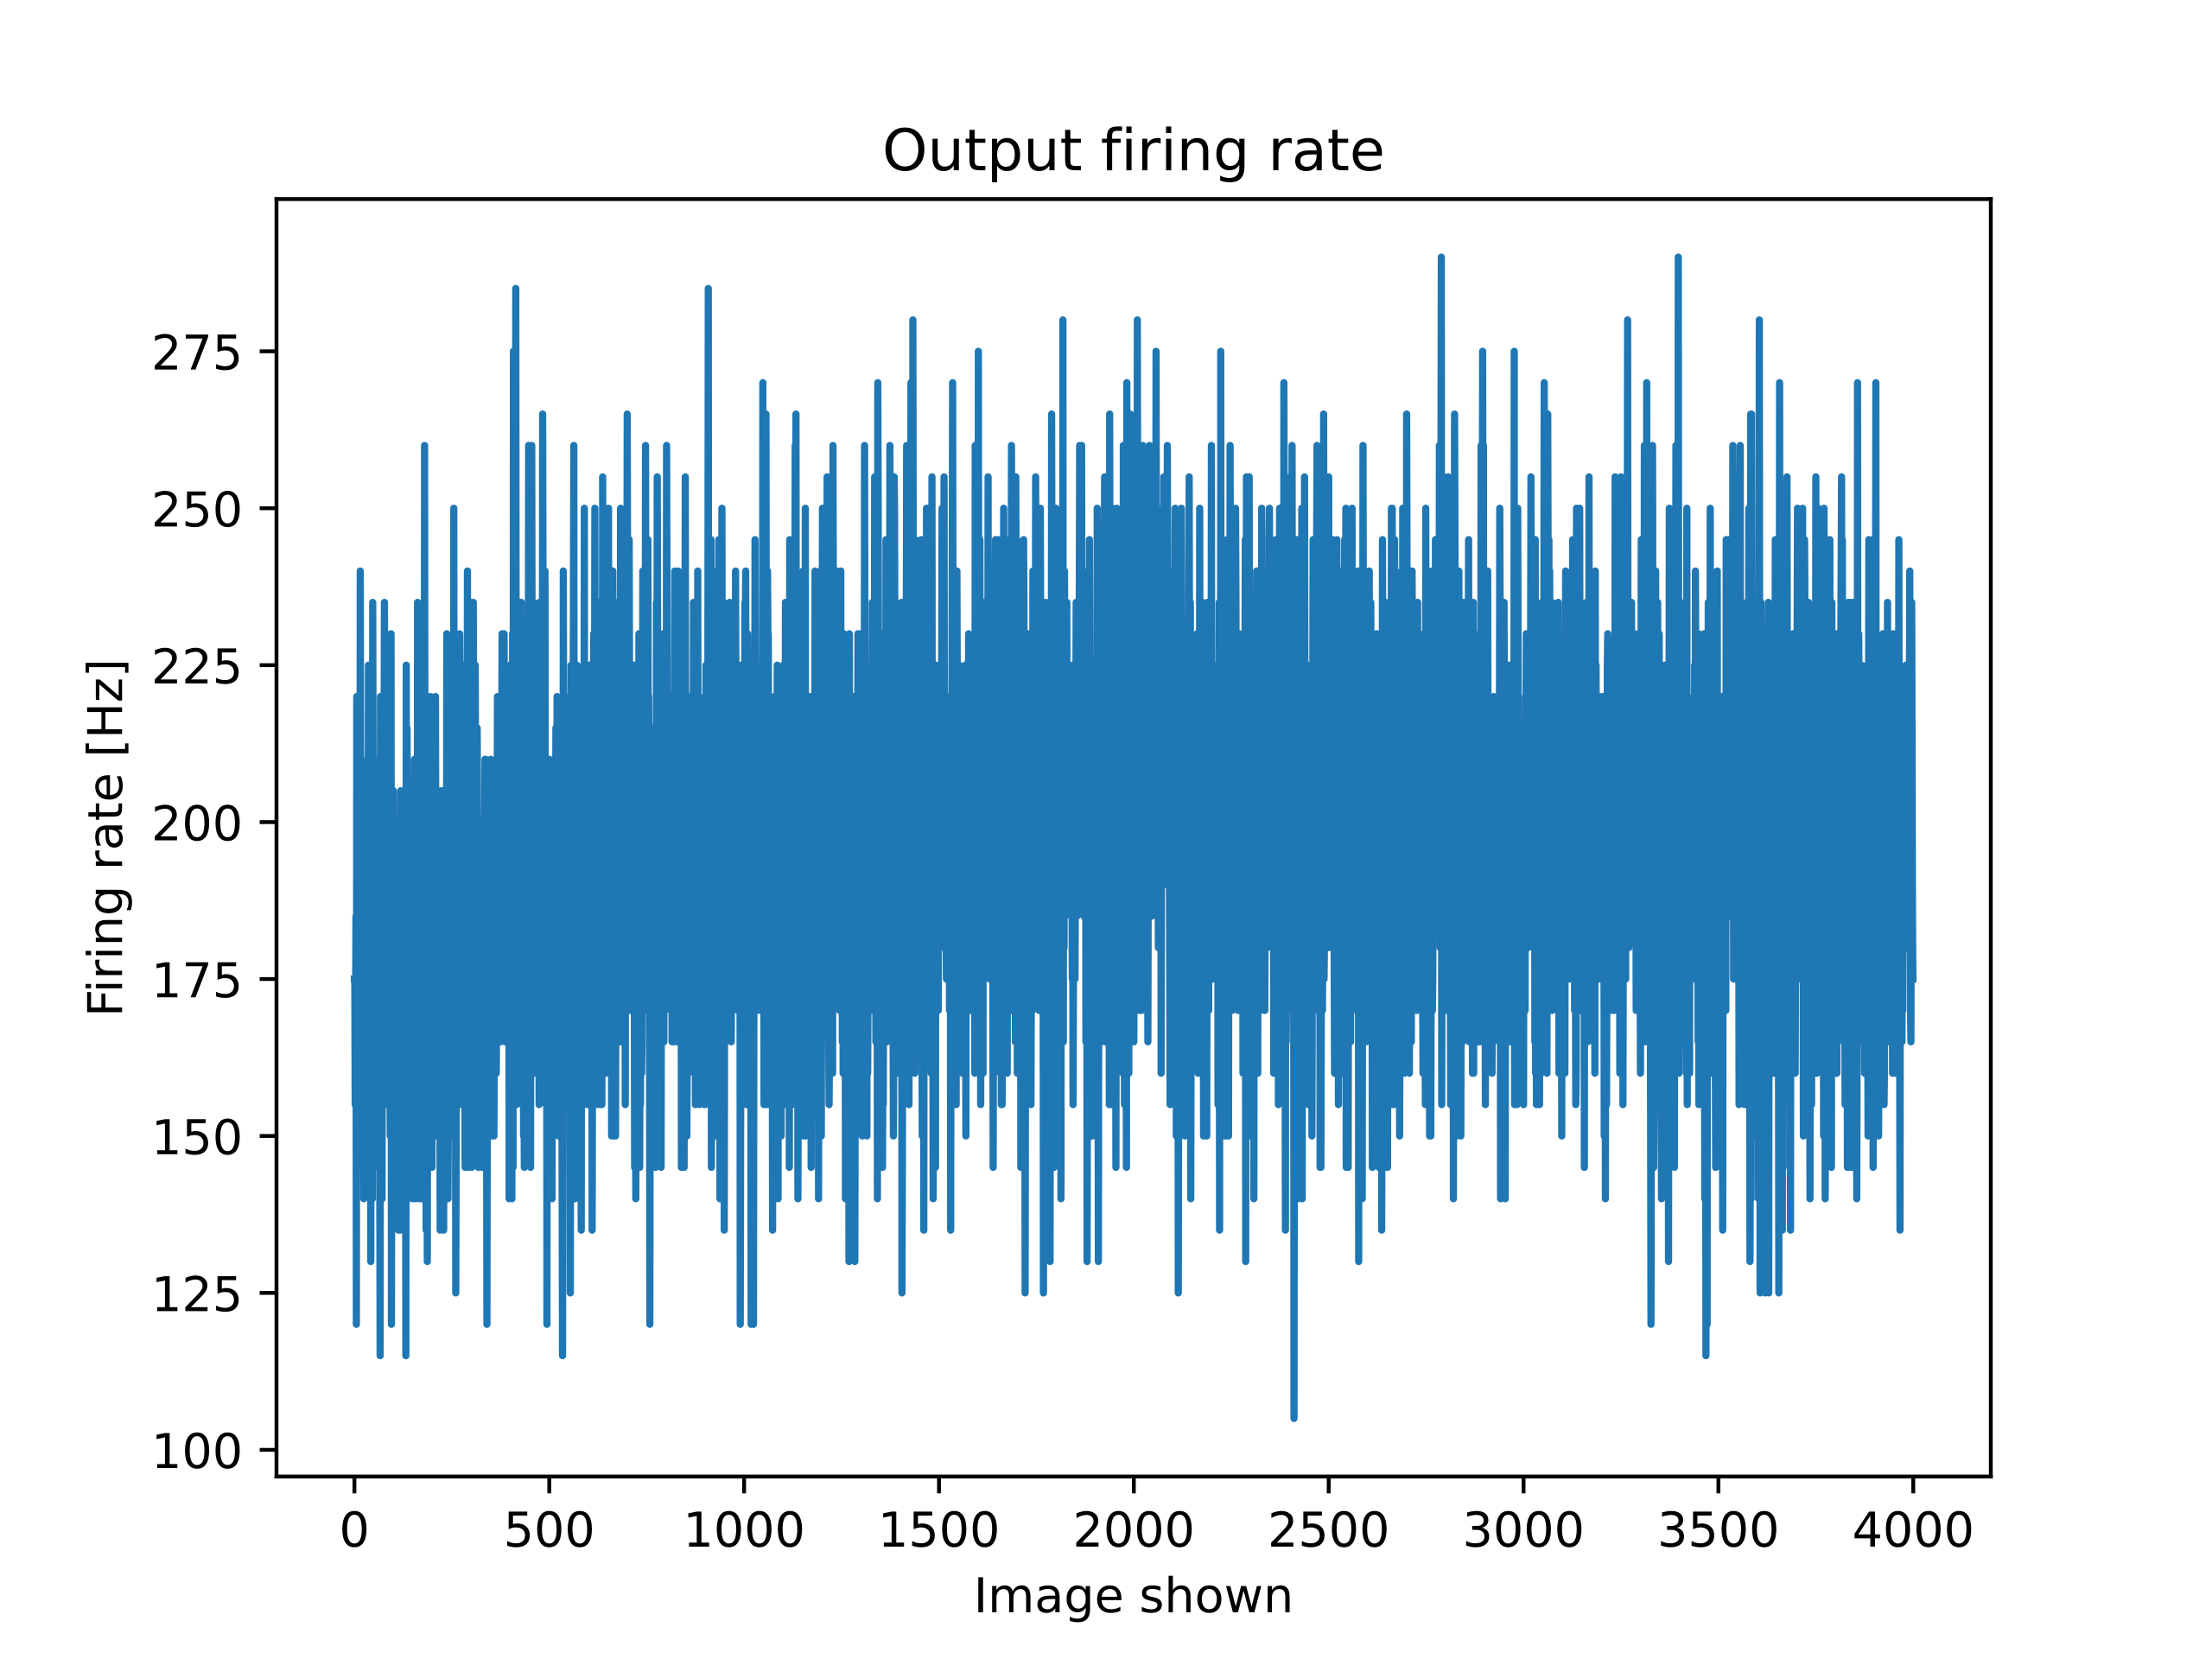
\includegraphics[width=\linewidth]{figures/angleAdaptiveInh/outputFiringRate.png}
  \caption{ Firing rate of all output neurons combined over the training process. }
  \label{fig:angleNetworkAdaptiveInhibitionOutputFiringRate}
\end{figure}

\begin{figure}
  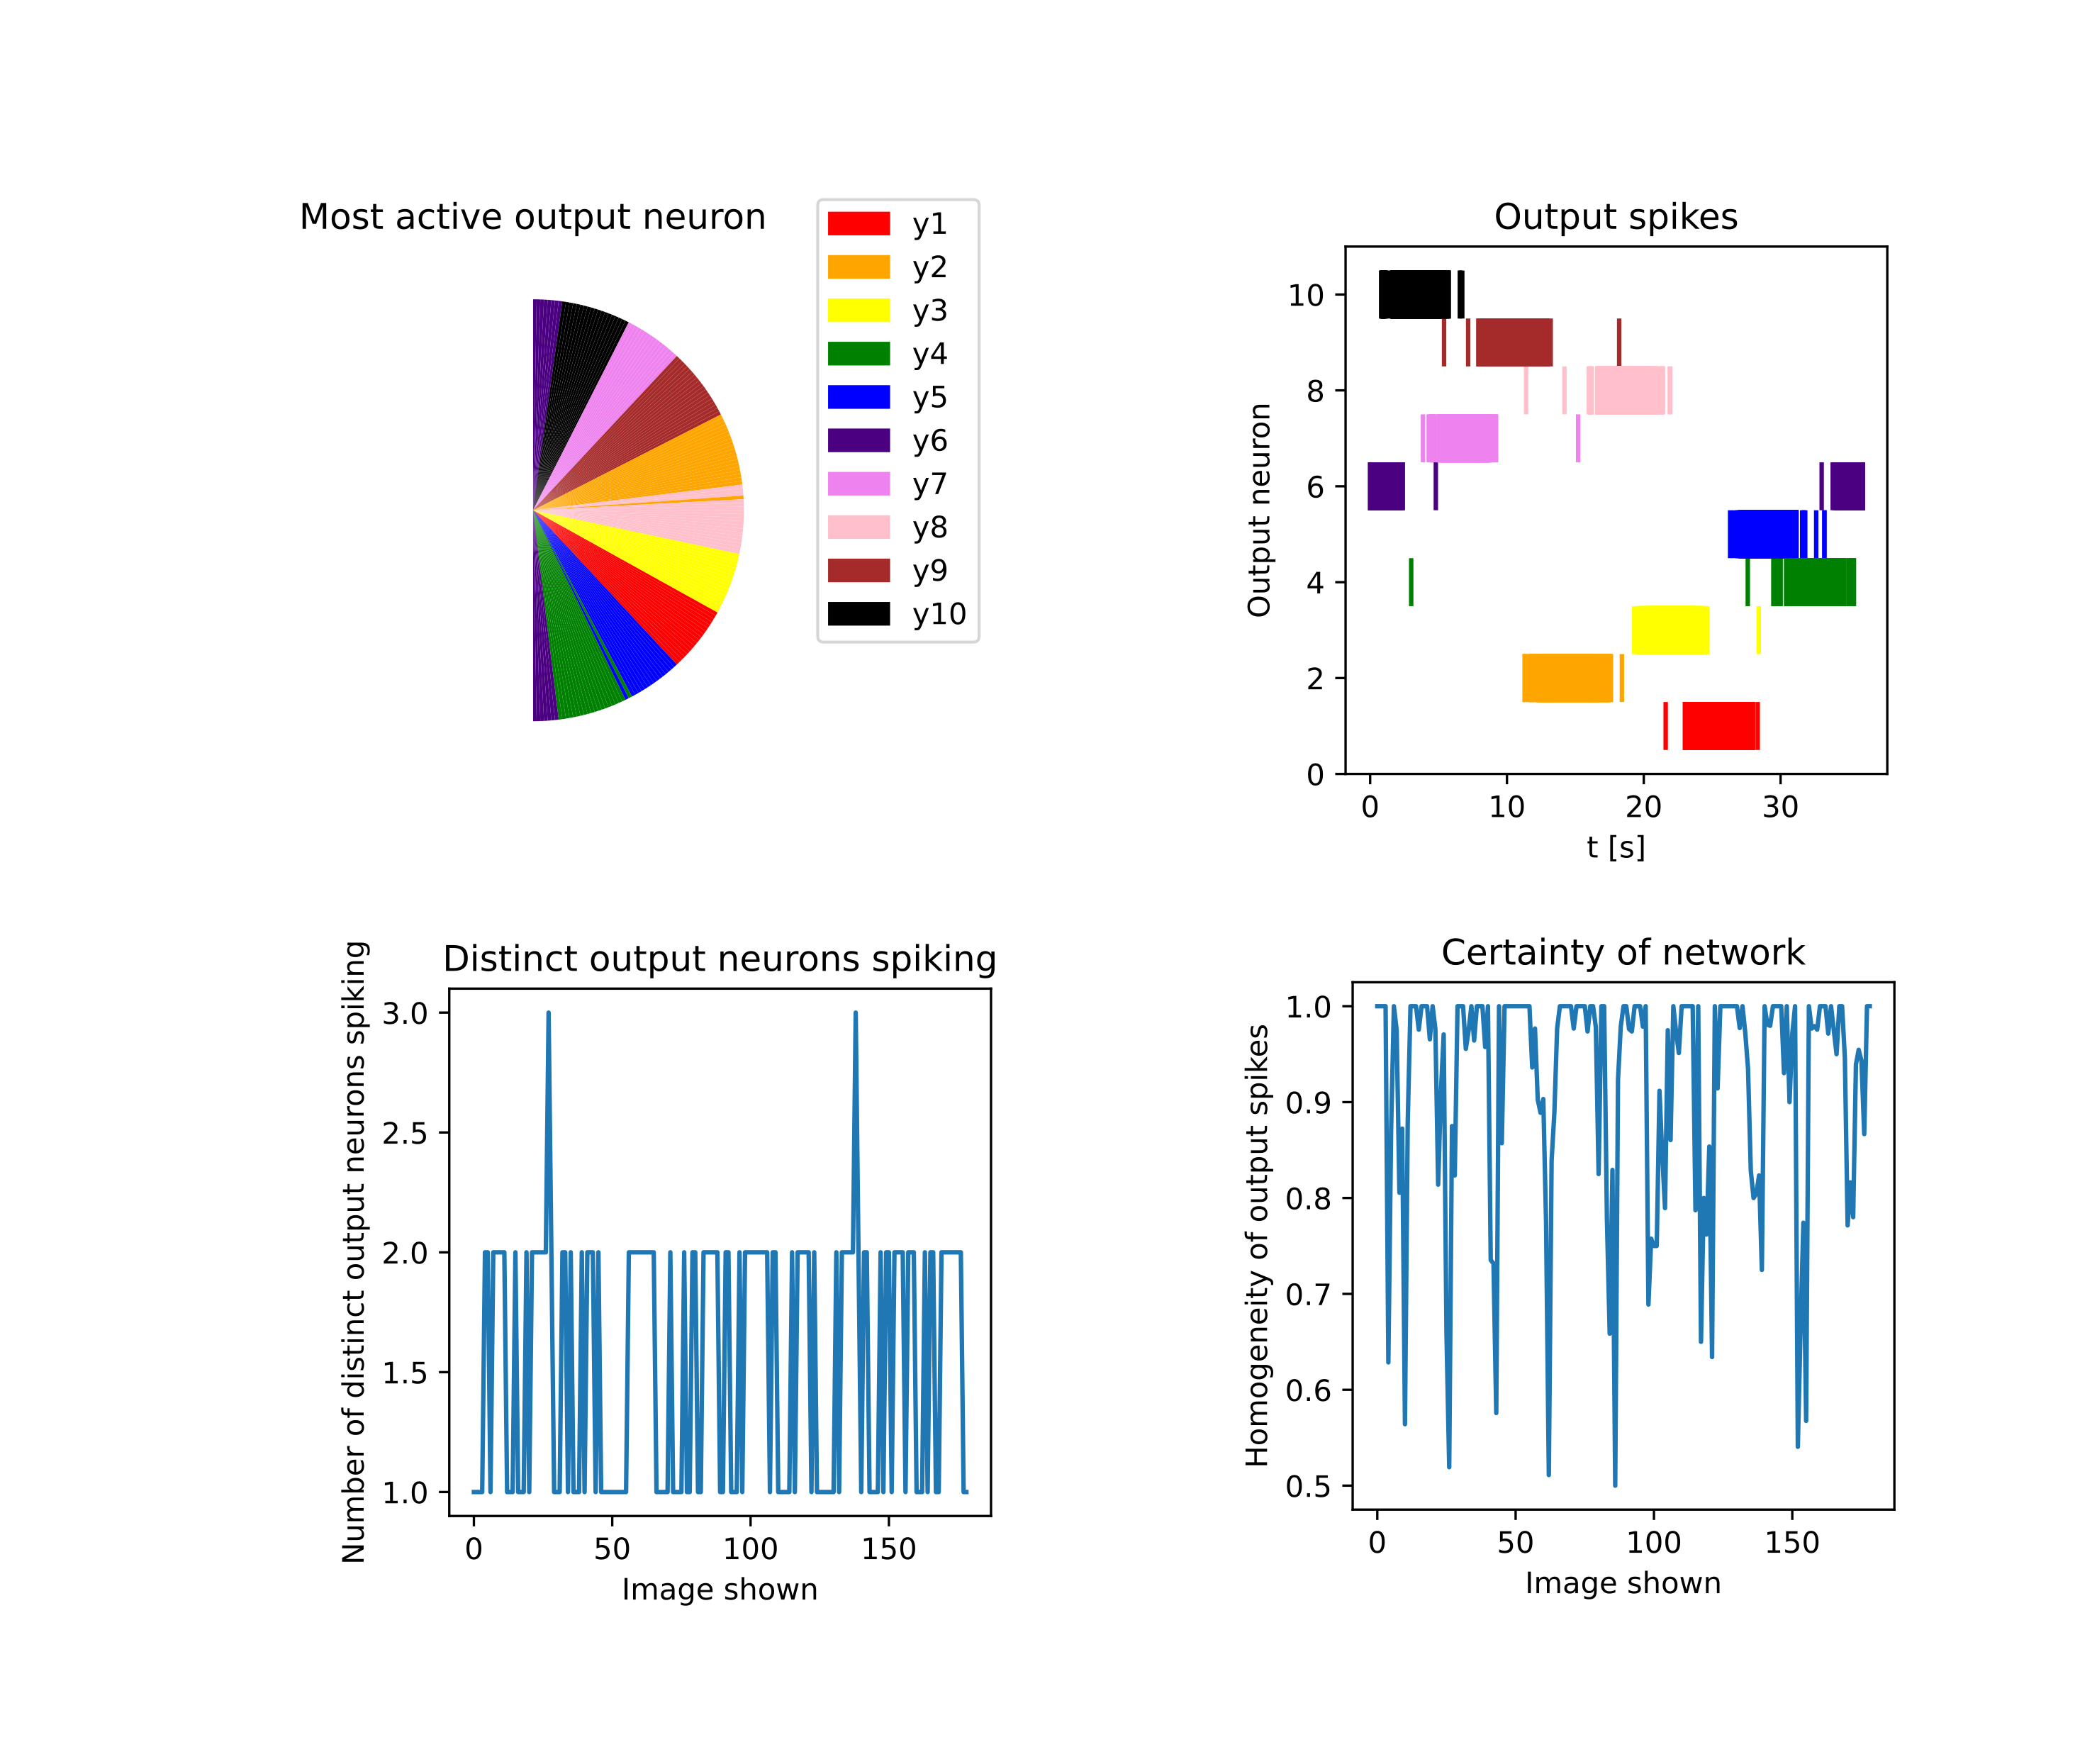
\includegraphics[width=\linewidth]{figures/angleAdaptiveInh/validation.png}
  \caption{\textbf{Validation.} \textbf{A} Most active output neuron depending on orientation of the training image. Training images were shown for 200 ms of each possible orientation in 1° steps. \textbf{B} Spike activity expressed by the output neurons during the validation process described in (\textbf{B}). \textbf{C} Number of distinct output neurons active during the presentation of each validation image. \textbf{D} Proportion (accuracy) of most active output neuron to activity of all other output neurons during the presentation duration of each training image.}
  \label{fig:angleNetworkAdaptiveInhibitionValidation}
\end{figure}
\section{Experiment 1: Horizontal and vertical bars}
\label{section:horvertAdaptiveInhibition}

\subsection{Introduction}

For this experiment images of either horizontal or vertical bars will be shown to the WTA network. Through unsupervised learning the output neurons will learn to cluster the images together, depending on the orientation and position of the bars. The the learning of the network will be visualized and analysed.
Further, the effect of the prior neurons will be demonstrated by generating ambiguous images which show a horizontal and a vertical bar at the same time. The output of the network will be analysed, depending on the activity of the prior neurons. 

\subsection{Methods}

\paragraph{Input data}
Black bars with a width of seven pixels were drawn onto a white background with a size of 35 x 35 pixels. The bars could be oriented either horizontally or vertically. The network was supposed to form ten different groups within these images, five with a horizontal orientation and five with a vertical orientation. With a given bar width of seven pixels the image height and width were determined as 35 pixels, to yield equally sized groups. Assuming equally sized groups and starting to count from position 0 the centers of the groups should then be at positions 3, 10, 17, 24, 31. The orientation of the training images was chosen randomly via a uniform distribution. The positions of the bars in the training images were uniformly distributed along the 35 pixels of either axis. To simulate noise each pixel of an image had a chance of ten percent to have its color flipped after the generation.
During the training of the network random images were generated and presented for 200 ms. As the simulation had a duration of 800 seconds this resulted in 4000 images being shown to the network. Examples of the input data can be seen in Figure \ref{fig:horvertImages}. To show the value of the added a-priori information, validation images with two bars forming a cross were also generated, seen in Figure \ref{fig:horvertTrainingCrossImage}. When shown to the network in the validation process the prior neurons were given the information that a cross is either of horizontal or vertical orientation.

\begin{figure}
  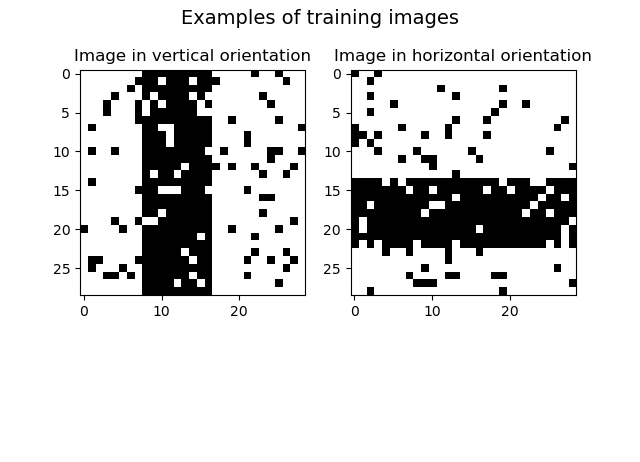
\includegraphics[width=\linewidth]{figures/horvert/horvertTrainingImages.png}
  \caption{Training images generated for experiment 1. One image of each possible orientation at a random position.}
  \label{fig:horvertImages}
\end{figure}

\begin{figure}
\centering
  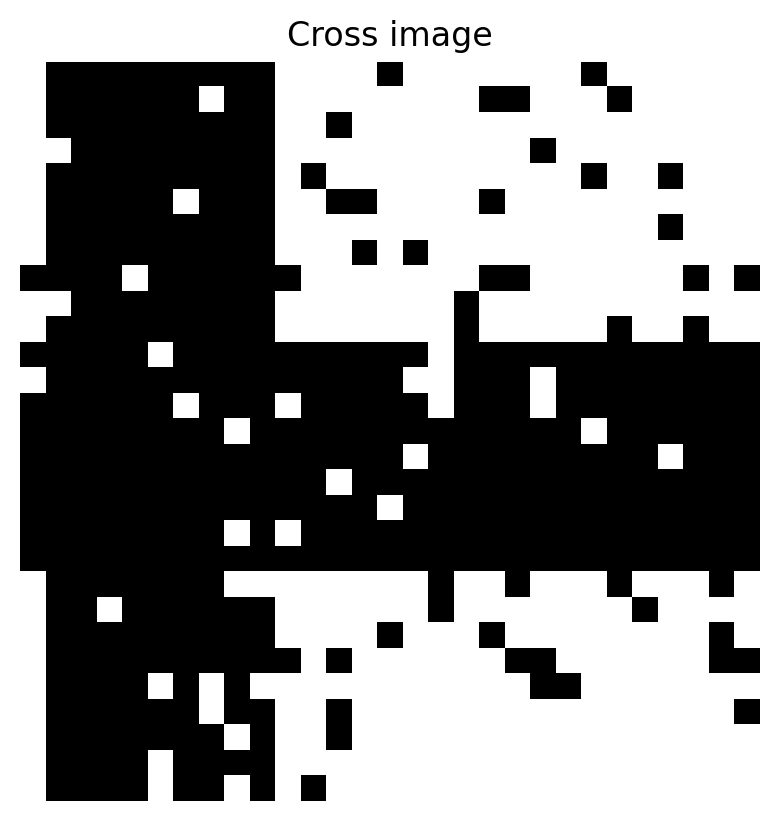
\includegraphics[width=0.6\linewidth]{figures/horvert/horvertTrainingCrossImage.png}
  \caption{Generated cross image which can represent either horizontal or vertical orientation.}
  \label{fig:horvertTrainingCrossImage}
\end{figure}

\paragraph{Network architecture}

As every pixel of an image was connected to two input neurons the network had 2450 input neurons. Each of these neurons had a firing frequency $f_{input}$ of 20 Hz, when in the active state. Then there were ten output neurons, one for each possible group. Lastly, there were two equal sized groups of prior neurons with firing frequencies $f_{prior}$ of 200 Hz. This firing frequency was chose as high plausible value to keep the needed number of prior neurons small compared to the number of input neurons. During training the first group $z^h$ was active when the image was of horizontal orientation and the other group $z^v$ was active for vertical orientation. The number of prior neurons had to be determined via grid search, as they needed to be set at values where the impact of the a-priori information is neither too strong nor too weak.

\paragraph{Network and hyperparameters}

The simulation of the experiment was performed in time steps of 1 ms. This step size was used for all experiments. As given by \citet{nessler} the time window $\sigma$ was 10 ms, the time constant for the rise of the EPSPs $\tau_{rise}$ was 1 ms and the time constant for the decay of the EPSPs $\tau_{decay}$ was 15 ms. Before performing this experiment, Experiment 2 of \citet{nessler} was reproduced to validate that the implementation of the simulation was correct. This proof of concept was omitted in this work, however within it the weight shift hyperparameter $c = 20$ and the learning rate $\lambda = 10^-3$ were determined via grid search. These hyperparameter values were reused for this experiment as the input data, as well as the network architecture, were similar.

\subsection{Results}

First different numbers of prior neurons were tested. Simulations with 10, 20, 50, 100 and 200 prior neurons were performed. For 50, 100 and 200 prior neurons the training process was impaired by the activity of the prior neurons. Some output neurons were responding to too large areas, while other prior neurons were not responding to any specific areas at all. This happened for example because the first output neuron that generated a spike for a horizontal bar got reinforced by the prior neurons to respond to all horizontal bars, no matter the position. Thus other output neurons were less likely to respond to horizontal bars, resulting in output neurons that were not responding to any specific orientation or area at all. With a number of 10 and 20 prior neurons each of the output neurons learned to respond to coherent areas of the images. The prior neurons also learned to respond to either horizontal or vertical images. To maximize the impact of the a-priori information the validation of the network was performed with 20 prior neurons, as it was the largest number that resulted in a properly trained network. The results of the training process can be seen in Figure \ref{fig:horvertAdaptiveInhibitionTraining}. In Figure \ref{fig:horvertAdaptiveInhibitionTraining} A examples of input images are shown. The bars were positioned without overlapping each other, thus showing the optimal areas output neurons should learn to respond to. The areas that output neurons did learn to respond to can be seen in the visualization of the input weights in Figure \ref{fig:horvertAdaptiveInhibitionTraining} B. It can be seen that the training was successful as five output neurons responded to horizontal bars and the other five to vertical bars. Furthermore each output neuron responded to different areas of the input image and there was little overlap between each other. The training progress of the network is given in Figure \ref{fig:horvertAdaptiveInhibitionTraining} E. When the network has completed the training it should mostly have only one or two output neurons being active for any input image. Although, there may be more active output neurons sporadically, due to the stochastic nature of the model. According to this plot the training process could have been stopped earlier after 2000 shown images. However, as there was no danger of overfitting the data more images were shown, to ensure that the network was always finished with the training when the simulation stopped. In Figure \ref{fig:horvertAdaptiveInhibitionTraining} F the relative activity of the most active output neuron can be seen. Firstly it can also be used to judge the progress of the training process, as it increased over time. Furthermore it can also be seen as a measure of how clearly an image belonged to the area the most active output neuron responded to. If the position of an image was exactly in the middle of the learned area of the most active output neuron the relative activity should be one. However, when the position was on the border between two learned areas of output neurons the relative activity should only be 0.5, as the image belonged to both areas. The learned prior weights can be seen in Figure \ref{fig:horvertAdaptiveInhibitionpriorWeights}. There it can be seen that the first 10 prior neurons learned the same pattern, as all of them were in an active state whenever vertical bars were shown to the network. When comparing these prior weights to the input weights in Figure \ref{fig:horvertAdaptiveInhibitionTraining} B it can be seen that the five highest prior weights of each prior neuron are between themselves and output neurons that learned to respond to vertical bars. The last 10 prior weights showed exactly the opposite pattern, having their five highest weight values between themselves and output neurons that responded to horizontal bars.

\begin{figure}
  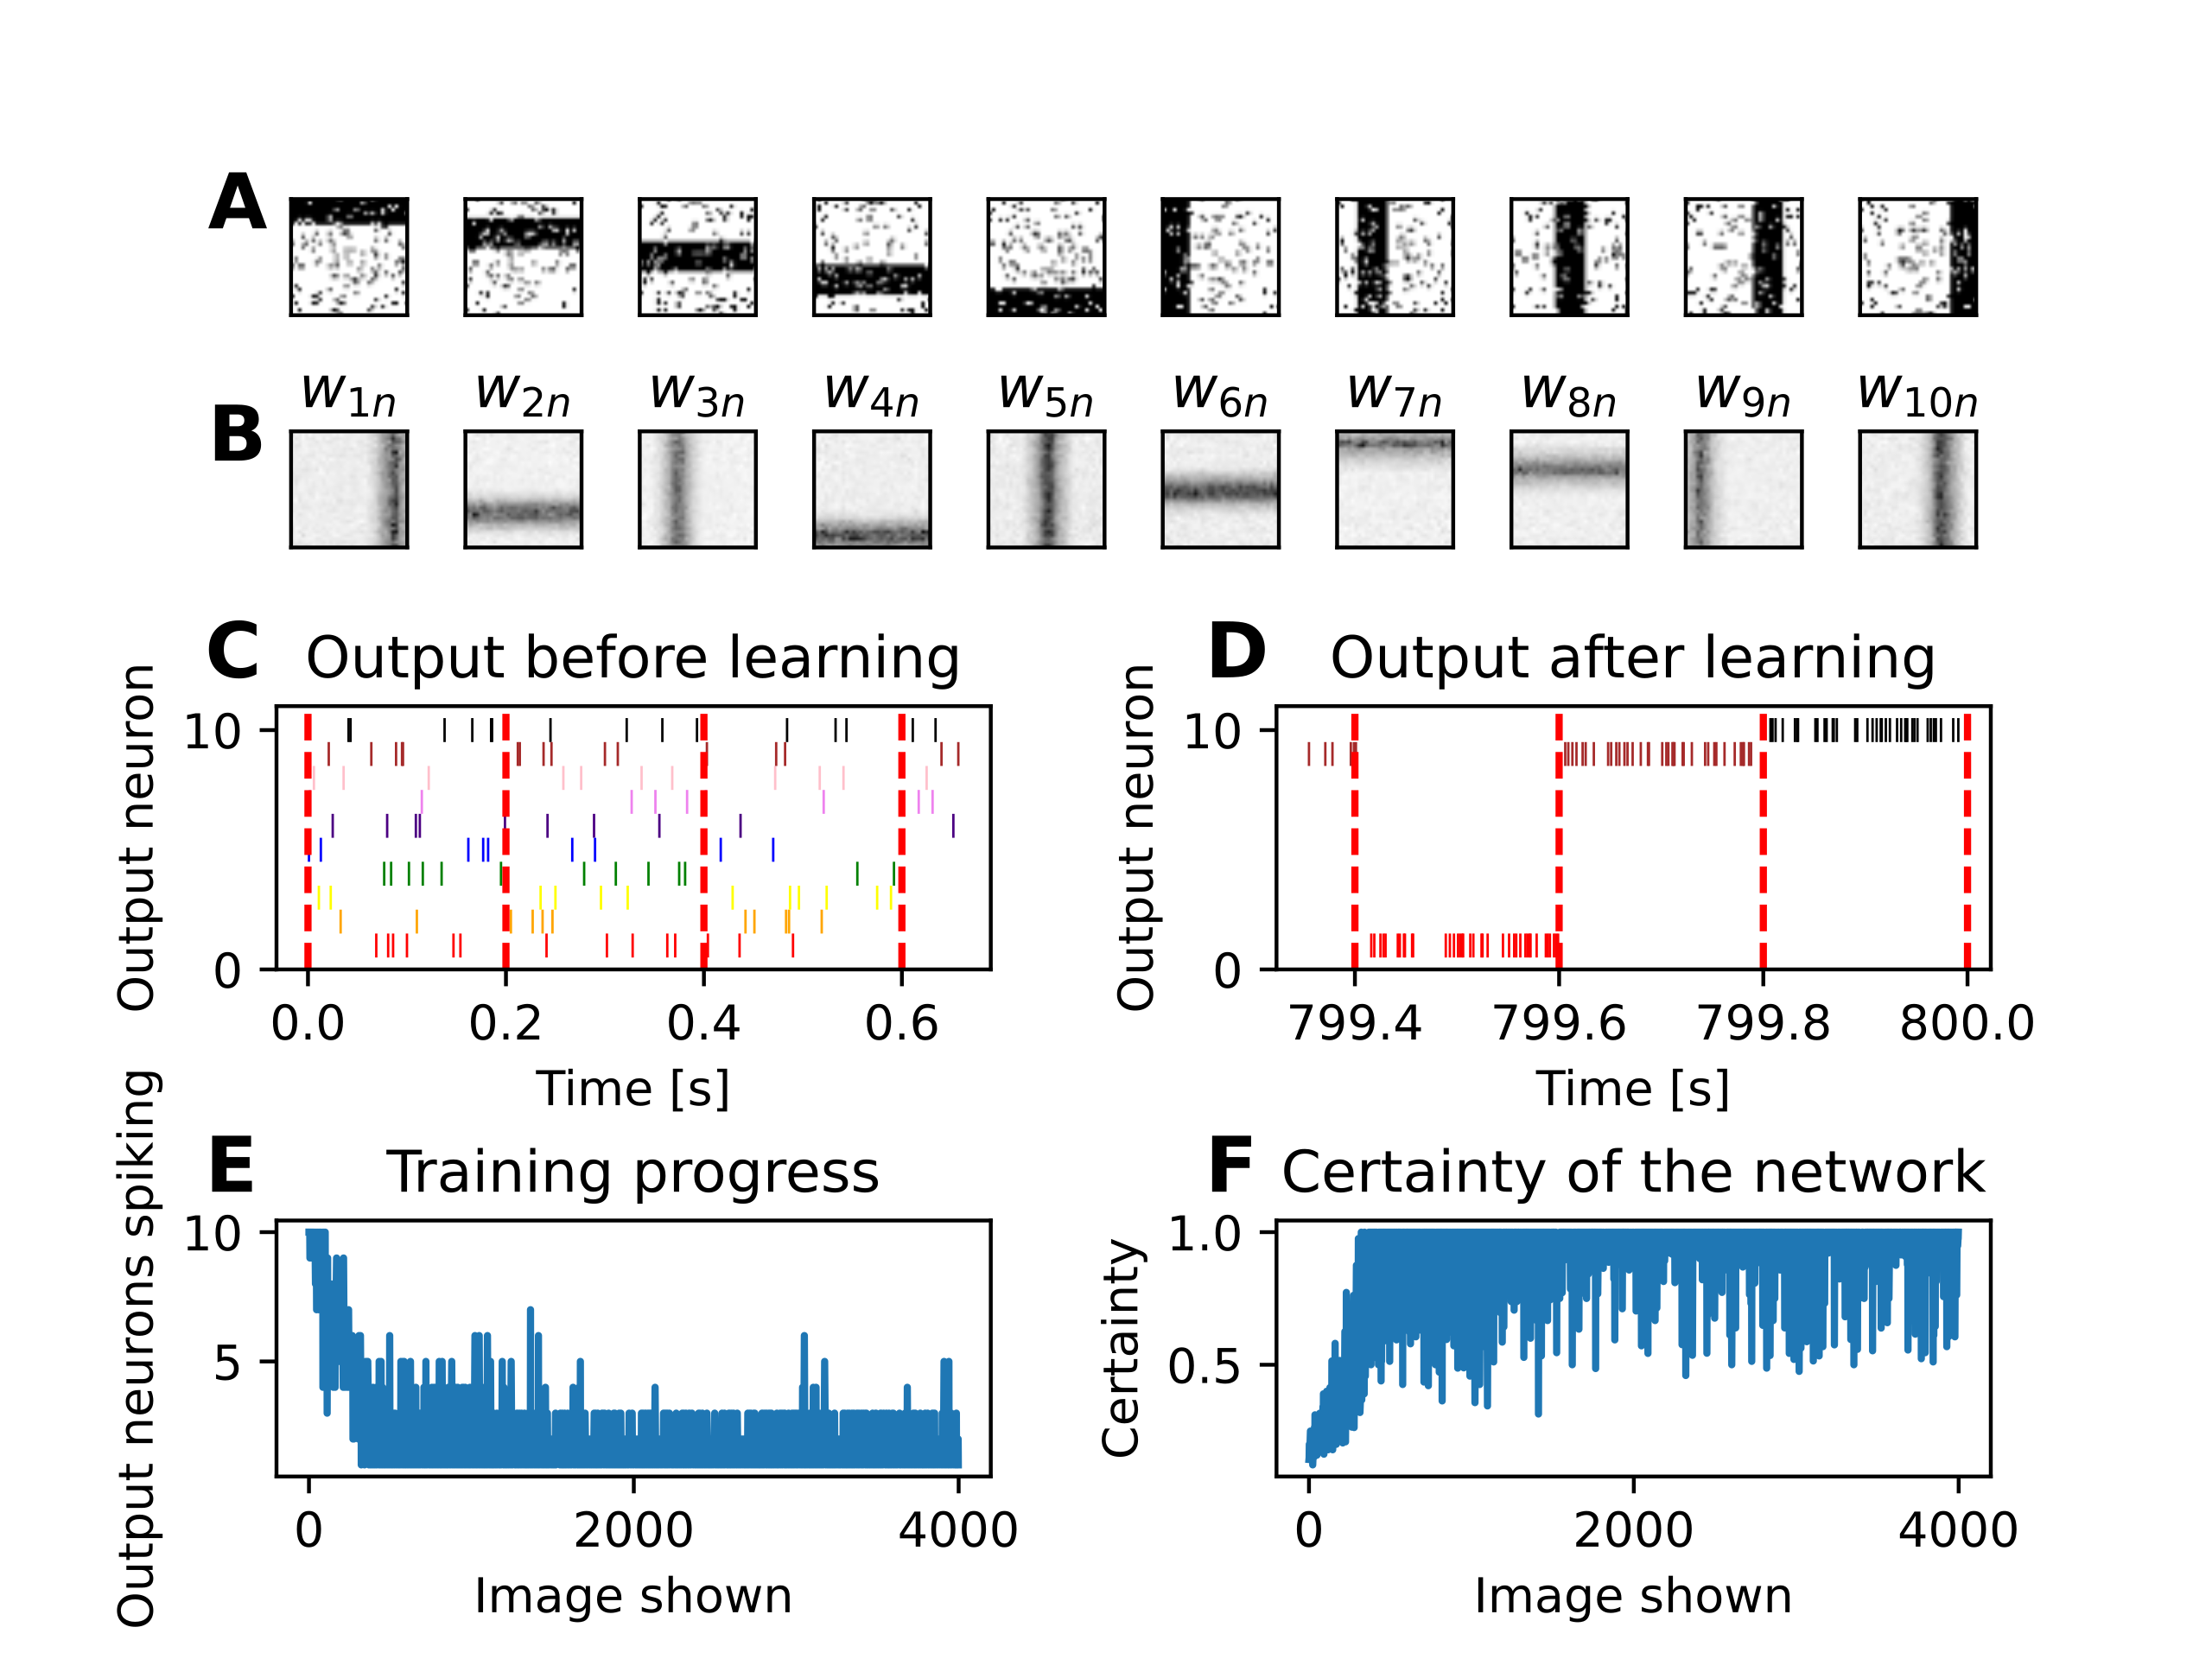
\includegraphics[width=\linewidth]{figures/horvertAdaptiveInh/trainingPlot.png}
  \caption{\textbf{Training with 20 prior neurons.} \textbf{A} Examples of 35 x 35-pixel input images of horizontal and vertical bars with background noise. They were positioned without overlapping each others bars, thus showing the optimal areas output neurons should learn to respond to. \textbf{B} Learned weights of the connections between input the neurons that were active for black pixels of the input image and output neurons. As each there was one such input neuron per pixel of the image the weights could be plotted in the same format as the image to easily interpret them. \textbf{C, D} Spike activity expressed by the output neurons before and after the training of the network. \textbf{E} Number of active output neurons during the presentation duration of each training image. \textbf{F} This shows the number of spikes the most active output neuron generated, relative to the number of spikes all other output neurons generated combined. }
  \label{fig:horvertAdaptiveInhibitionTraining}
\end{figure}

\begin{figure}
  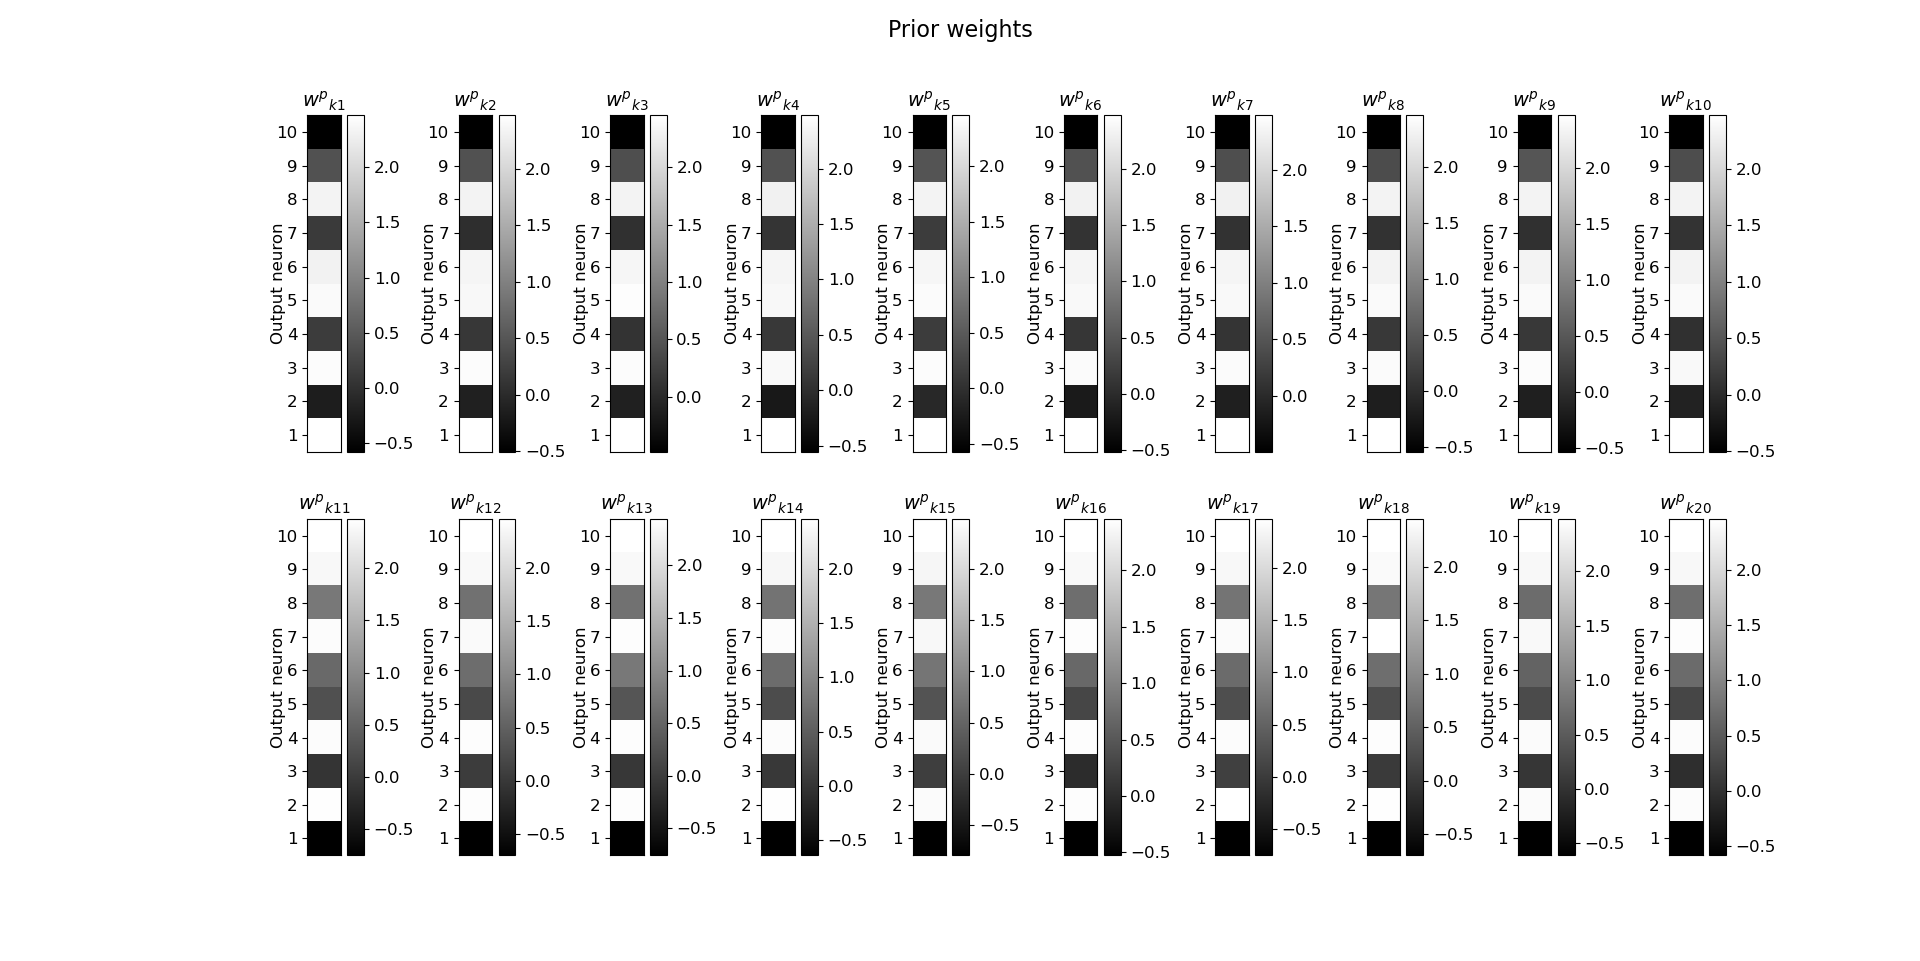
\includegraphics[width=\linewidth]{figures/horvertAdaptiveInh/priorWeights.png}
  \caption{ Learned weights of the connections between prior and output neurons. }
  \label{fig:horvertAdaptiveInhibitionpriorWeights}
\end{figure}

To validate the learned patterns the network was shown horizontal bars with a height of seven pixels with their centers at every possible position, beginning at position zero and incrementing in steps of one. Each image was shown for 200 ms each, while recording the output neuron activity. To visualize which output neuron is the most active for each position a horizontal bar with a height of one was drawn into a 35 x 35 pixel image, color-coded to represent the most active output neuron for that position. This can be seen in Figure \ref{fig:horvertAdaptiveInhibitionHorizontalValResults} A. $y_7$ and $y_{10}$ claimed areas with heights of eight pixels, while the areas of $y_9$ and $y_4$ had only a height of six pixels. Only $y_2$ had an area height of the expected seven pixels. These varying heights were expected to happen, due to the unsupervised learning method applied in this thesis. Depending on the randomly generated images the network received during the training process there may be more images on one side of the border between two output neurons than on the other side. This would result in the favoured neuron having stronger weights around the border area. Because of that the favoured neuron might end up claiming a larger active area.
The output spikes of the network can be seen in Figure  \ref{fig:horvertAdaptiveInhibitionHorizontalValResults} B. It can be seen that outside of the border areas between the output neurons there was mostly only one neuron active. However, shortly after two seconds $y_8$ was active. The time frame between 2 seconds and 2.2 seconds this happened in corresponds to position 10. $y_8$ should mostly be active for vertical bars, however its learned area has some overlap with with a horizontal bar at position ten and thus there is always a small chance for it to generate a spike. 
In Figure \ref{fig:horvertAdaptiveInhibitionHorizontalValResults} C the number of active output neurons for each position is given.  The validation process was repeated ten times and the mean and standard deviation of the number were calculated. In this plot four peaks appeared. These peaks are around the borders between the adjacent active areas of output neurons seen in Figure \ref{fig:horvertAdaptiveInhibitionHorizontalValResults} A. Around the border areas a number of active output neurons bigger than one was expected, as the horizontal bars reach into the areas of two output neurons at once. When looking at the number of active output neurons at position 10, which is approximately 1.1 with a high standard deviation, it shows that $y_8$ did not falsely learn to be active for horizontal bars, but rather that it was a stochastic outlier. Figure \ref{fig:horvertAdaptiveInhibitionHorizontalValResults} D shows the relative activity of the most active output neuron. Compared to Figure \ref{fig:horvertAdaptiveInhibitionHorizontalValResults} C it provides the additional information of how split the activity of neighbouring output neurons is in the border areas. For example it can be seen that at position 22 $y_4$ had a relative activity of 0.62. It was only barely able to be the most active neuron and might almost have had only an active area with a height of five pixels.

\begin{figure}
  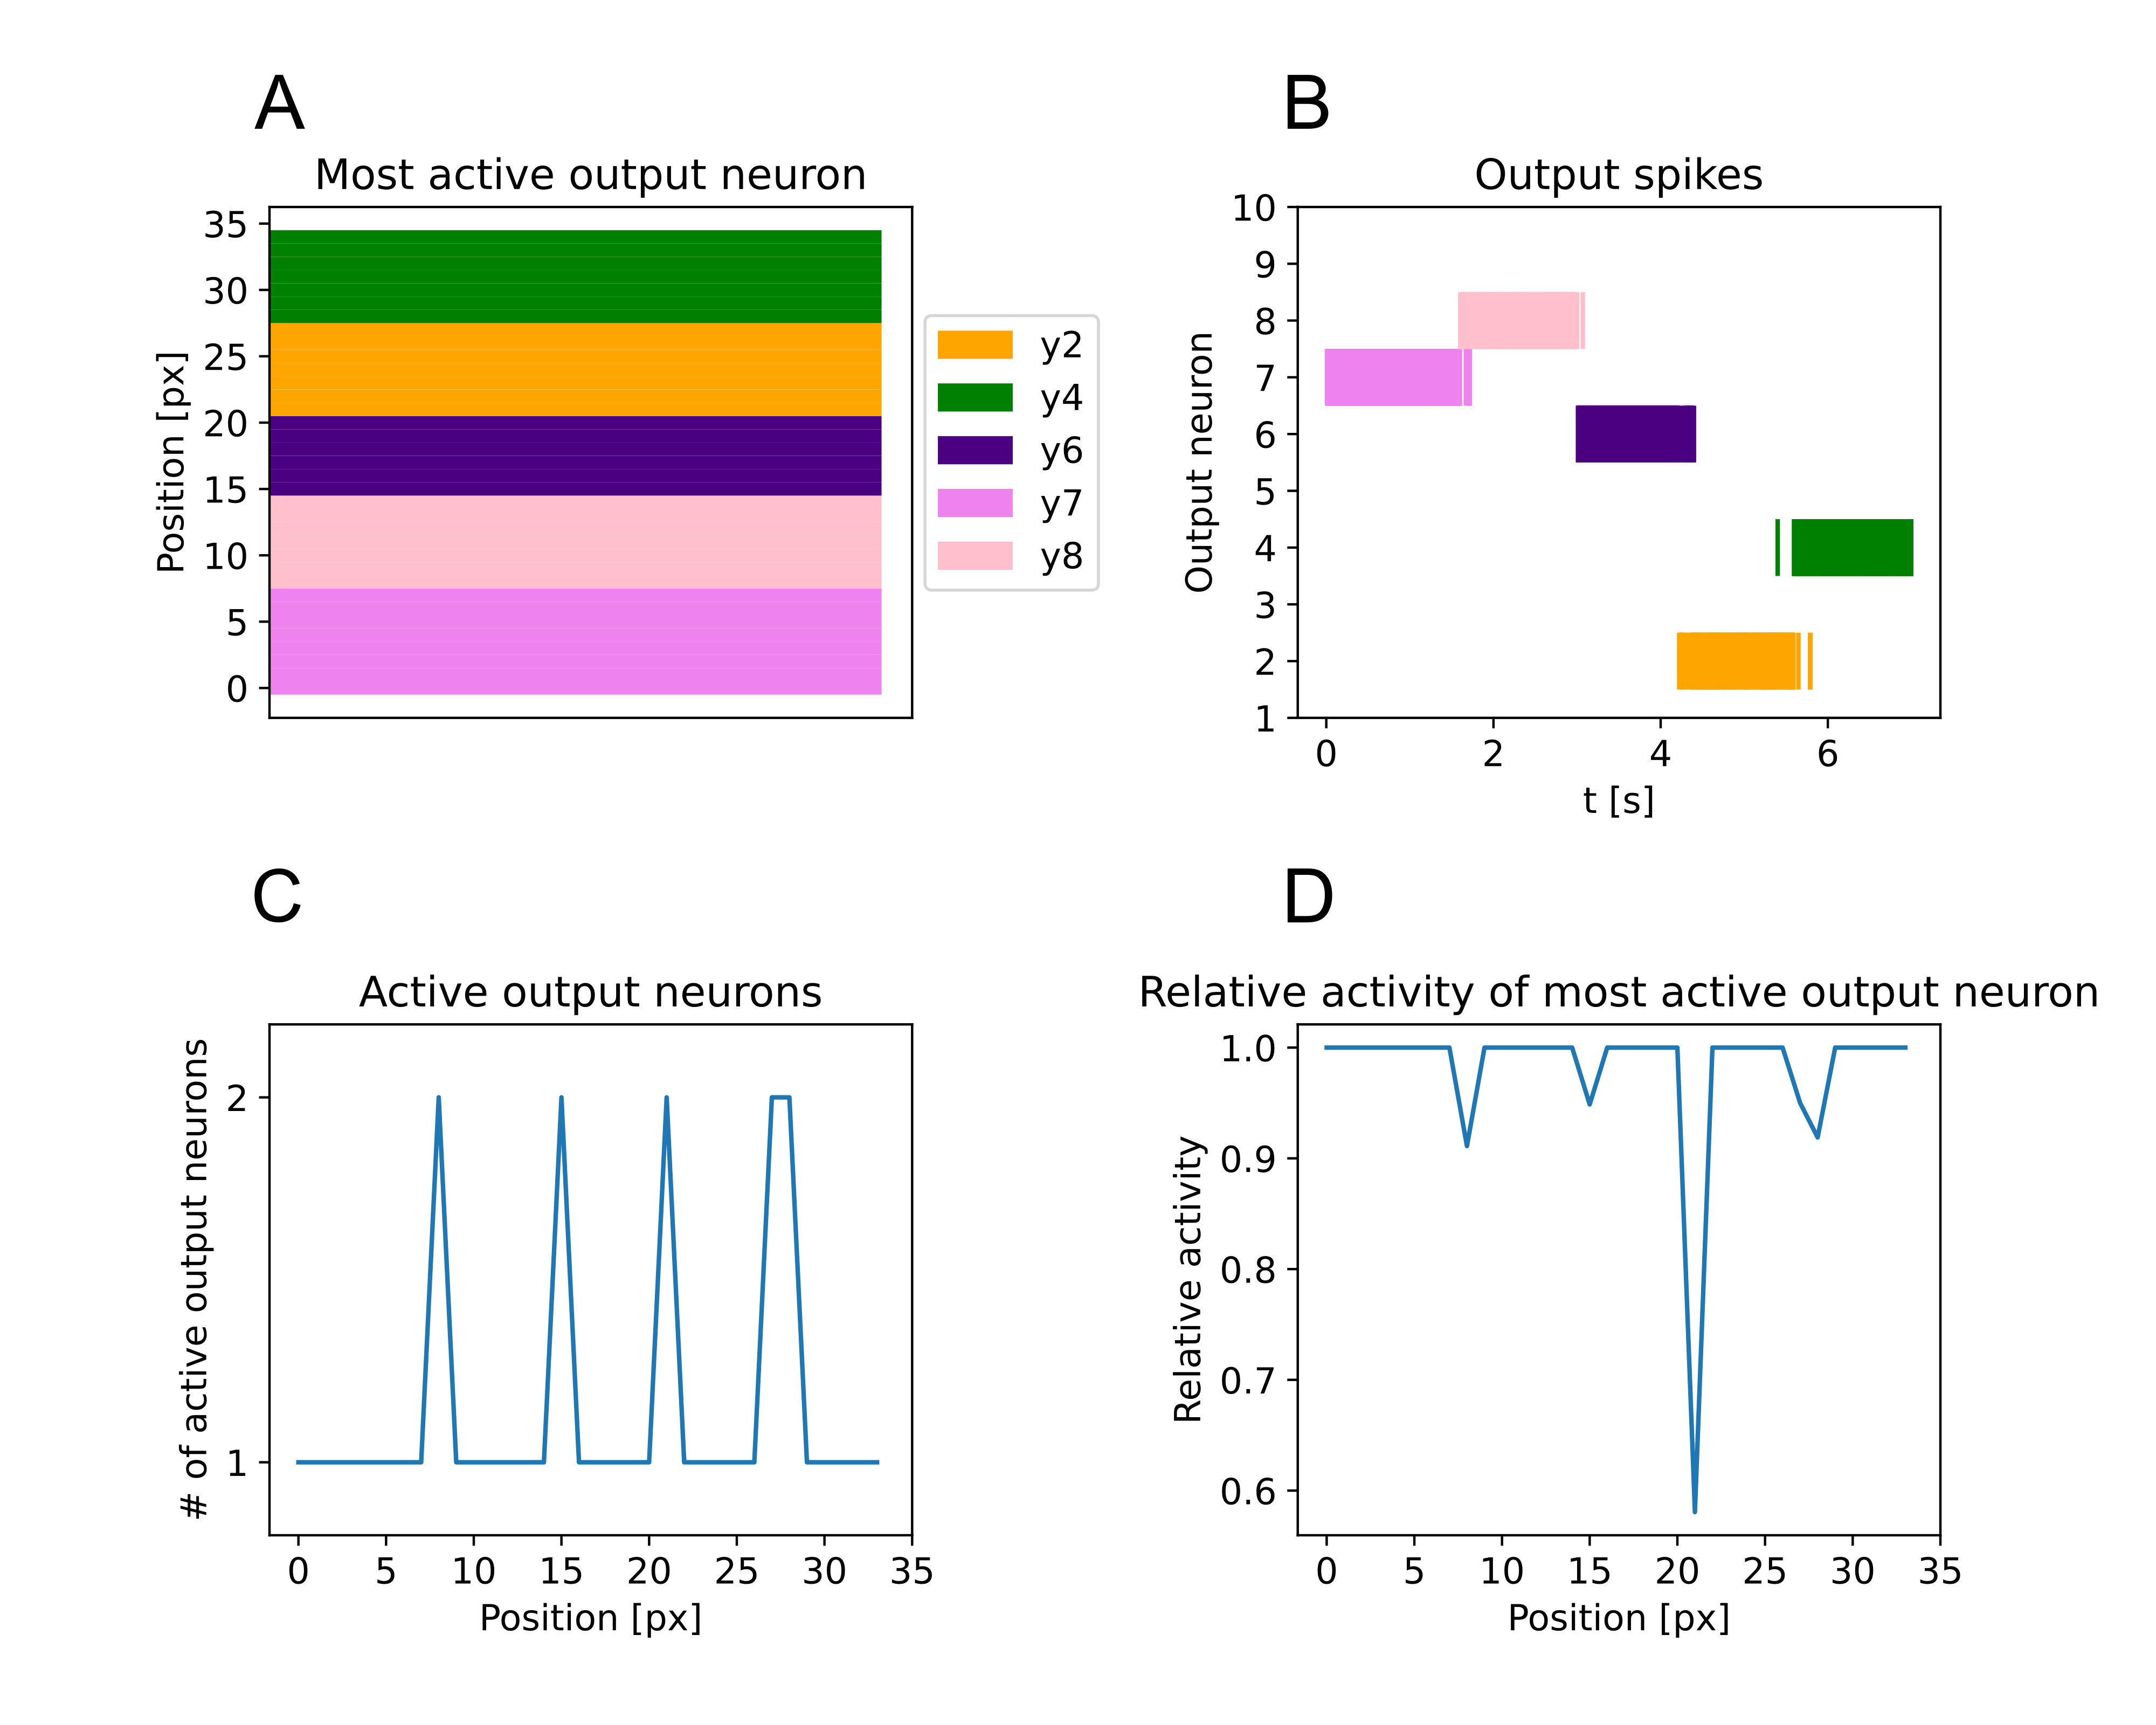
\includegraphics[width=\linewidth]{figures/horvertAdaptiveInh/horizontal_validation.png}
  \caption{\textbf{Horizontal validation.} Horizontal bars with a height of seven pixels were shown to the network at different positions. \textbf{A} Most active output neuron, depending on the vertical position of the center of a horizontal bar. \textbf{B} Output spikes during the validation process. The ticks of the x-axis are in steps of 0.2 seconds, thus each tick signifies the start of a new image being shown. \textbf{C} The mean number of active output neurons, depending on the vertical position of a horizontal bar. The standard deviation is given by the red bars. \textbf{D} This shows the of number of spikes the most active output neuron generated, relative to the number of spikes all other output neurons generated combined. The blue dots indicate the mean and the red bars the standard deviation. }
  \label{fig:horvertAdaptiveInhibitionHorizontalValResults}
\end{figure}

The validation process for the vertical bars was done analogously to the horizontal bars. Its results are given in Figure \ref{fig:horvertAdaptiveInhibitionVerticalValResults}. 
 
\begin{figure}
  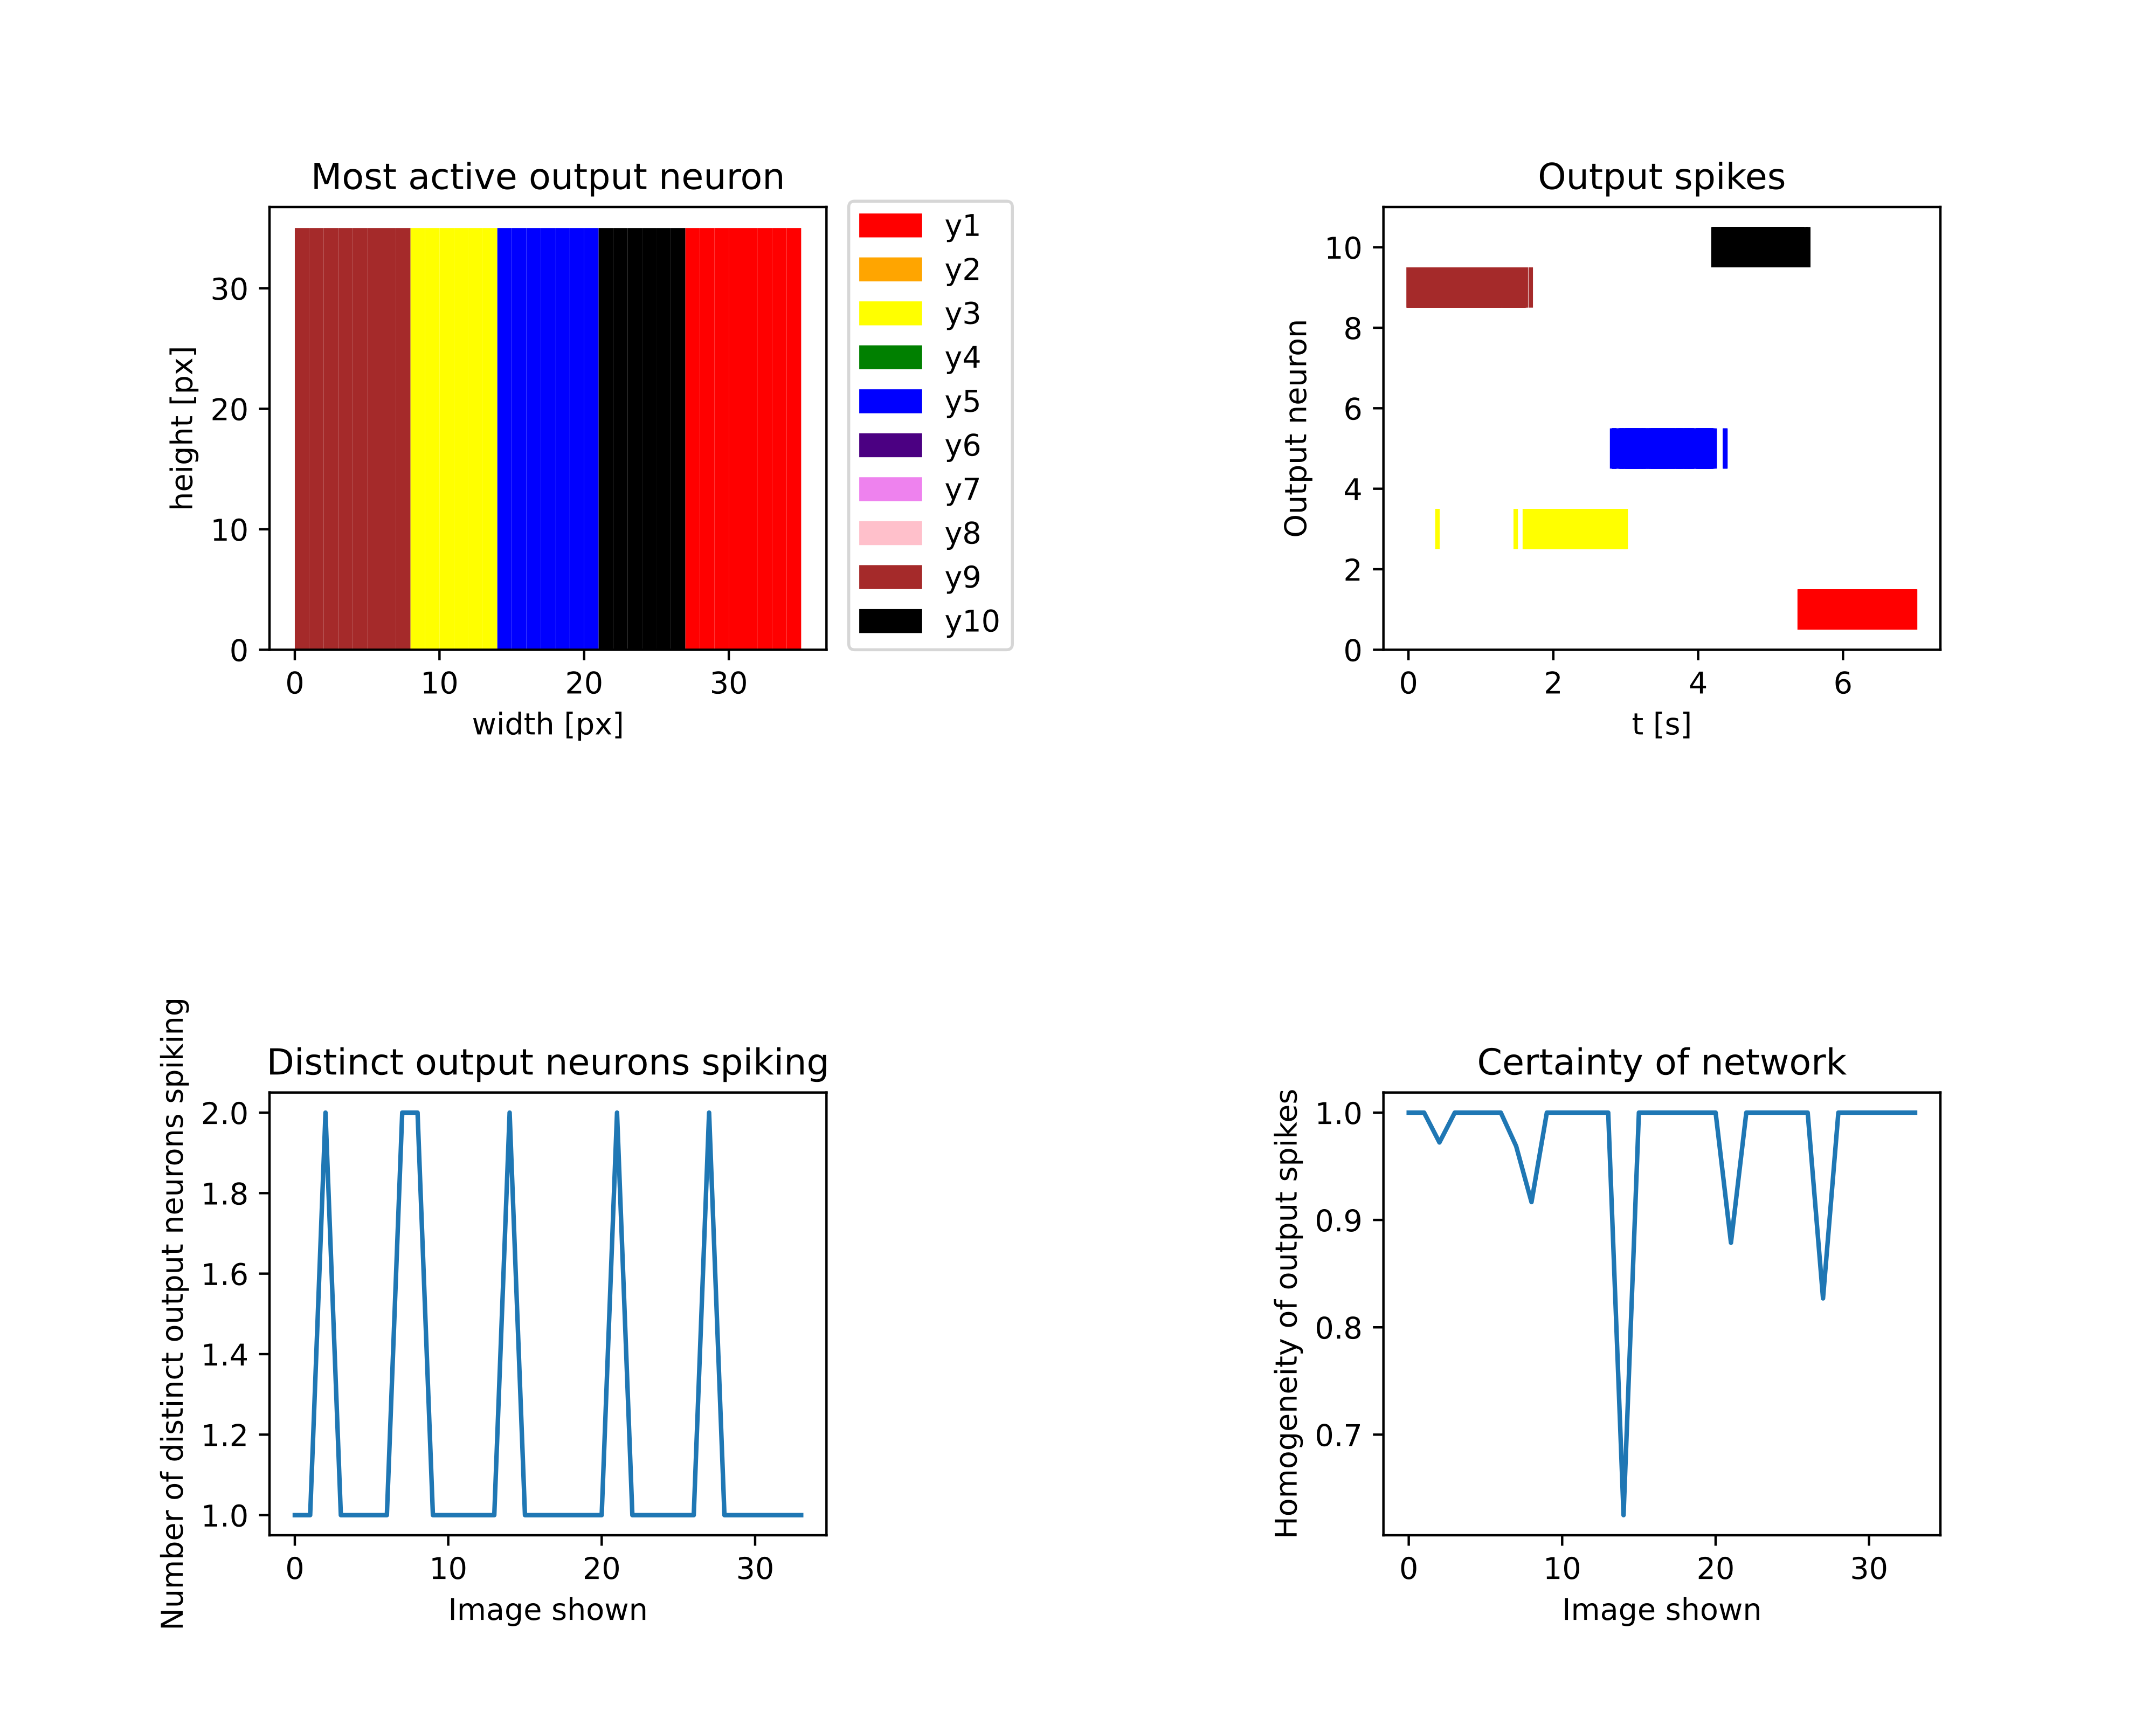
\includegraphics[width=\linewidth]{figures/horvertAdaptiveInh/vertical_validation.png}
  \caption{\textbf{Vertical validation.} Vertical bars with a height of seven pixels were shown to the network at different positions. \textbf{A} Most active output neuron, depending on the horizontal position of the center of a vertical bar. \textbf{B} Output spikes during the validation process. The ticks of the x-axis are in steps of 0.2 seconds, thus each tick signifies the start of a new image being shown. \textbf{C} The mean number of active output neurons, depending on the horizontal position of a vertical bar. The standard deviation is given by the red bars. \textbf{D} This shows the of number of spikes the most active output neuron generated, relative to the number of spikes all other output neurons generated combined. The blue dots indicate the mean and the red bars the standard deviation. }
  \label{fig:horvertAdaptiveInhibitionVerticalValResults}
\end{figure}

Next the impact of the prior was analysed. An image with a horizontal bar at position 12 and a vertical bar at position 5 on it was generated. First the prior neurons $z^v$ were activated and $z^h$ were deactivated. Then the image was shown to the network for 200 ms. After that the activity of the prior neurons was reversed and the image was shown again. The results can be seen in Figure \ref{fig:horvertAdaptiveInhibitionPriorValResults}. In that figure it can be seen that the output of the network completely changes depending of the prior activity. The prior neurons determine if the network focuses on the vertical or horizontal bar of the image.

\begin{figure}
  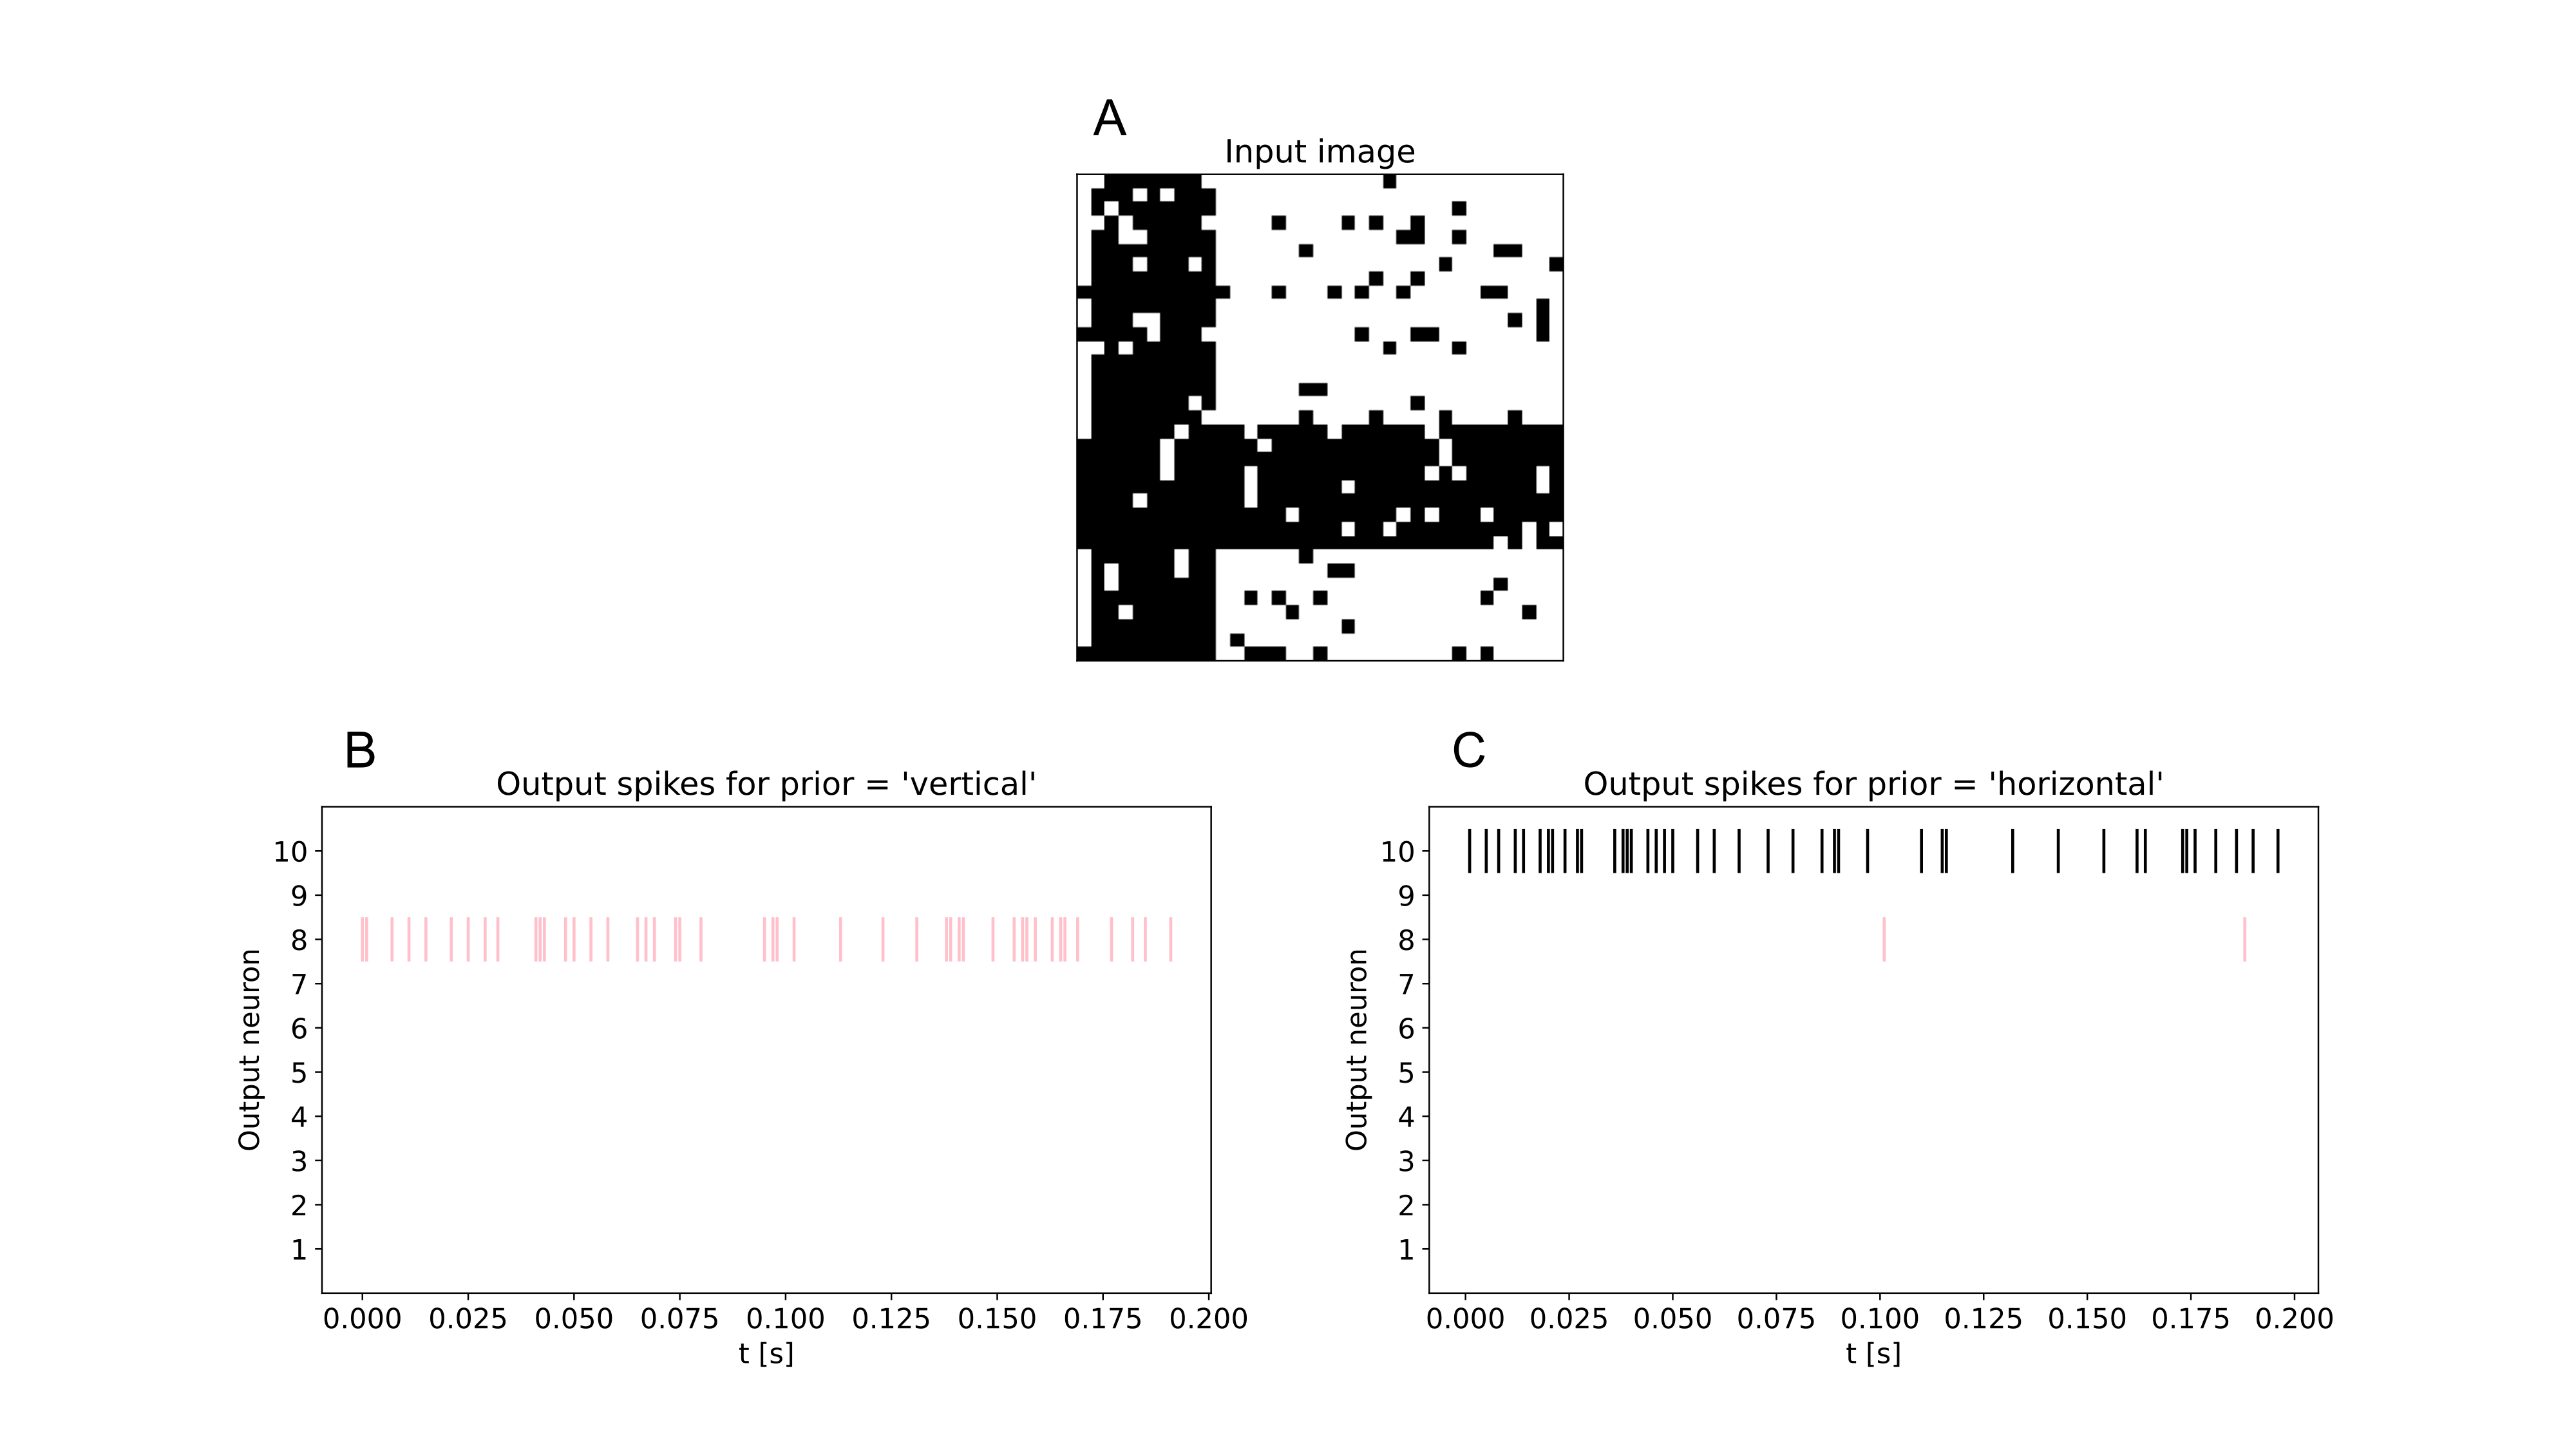
\includegraphics[width=\linewidth]{figures/horvertAdaptiveInh/20priors_pos5and12/crossValidation.png}
  \caption{\textbf{Impact of the prior Neurons.} \textbf{A} Validation image with a horizontal and a vertical bar on it. \textbf{B} Spiking activity of the output neurons with $z^v$ being active. \textbf{C} Spiking activity of the output neurons with $z^h$ being active. }
  \label{fig:horvertAdaptiveInhibitionPriorValResults}
\end{figure}

To further illustrate the dependence of the output on the prior the firing frequencies of the prior neurons were gradually changed. The starting firing frequency of $z^h$ was set to 200 Hz and to 0 Hz for $z^v$. For those firing frequencies a cross image was shown to the network for 200 ms. It had a horizontal bar at position 31 and a vertical bar at position 3. These position are as far at the edge of the image as possible, while still displaying the whole width of the bars. After each image presentation duration the firing frequency of $z^h$ was decreased by 1 Hz and increased by 1 Hz for $z^v$. The used cross image can be seen in Figure \ref{fig:horvertAdaptiveInhibitionVariablePriorResults} A. The firing frequency of the 2 most active output neurons depending on the firing frequency of $z^v$ can be seen in Figure \ref{fig:horvertAdaptiveInhibitionVariablePriorResults} B. At the beginning $y_2$, which represents the horizontal part of the cross image, was the most active neuron, which is correct as the prior neurons fully supported the horizontal interpretation of the input image. With rising firing frequency of $z^v$ the activity of the $y_2$ decreased and the activity of $y_8$ increased. This happened because the prior neurons gradually supported the interpretation of the image as vertical more and more. It was expected that the crossing point of the two graphs in Figure \ref{fig:horvertAdaptiveInhibitionVariablePriorResults} B would be at a firing frequency of $z^v$ of 100 Hz, however the graphs crossed at 58.6 Hz. In Figure \ref{fig:horvertAdaptiveInhibitionHorizontalValResults} D the relative activity of $y_2$ at the edge of the bar at position 28 was 0.79. In Figure \ref{fig:horvertAdaptiveInhibitionVerticalValResults} D the relative activity of $y_8$ at the edge of the bar at position 6 was 1.0. $y_8$ has a higher relative activity at that position than $y_2$ at position 28, because $y_8$ has an  active area of width 8, making position 6 not the border of the active area. Due to the larger active area of $y_8$ the crossing point shifted in favour of $y_8$.

\begin{figure}
  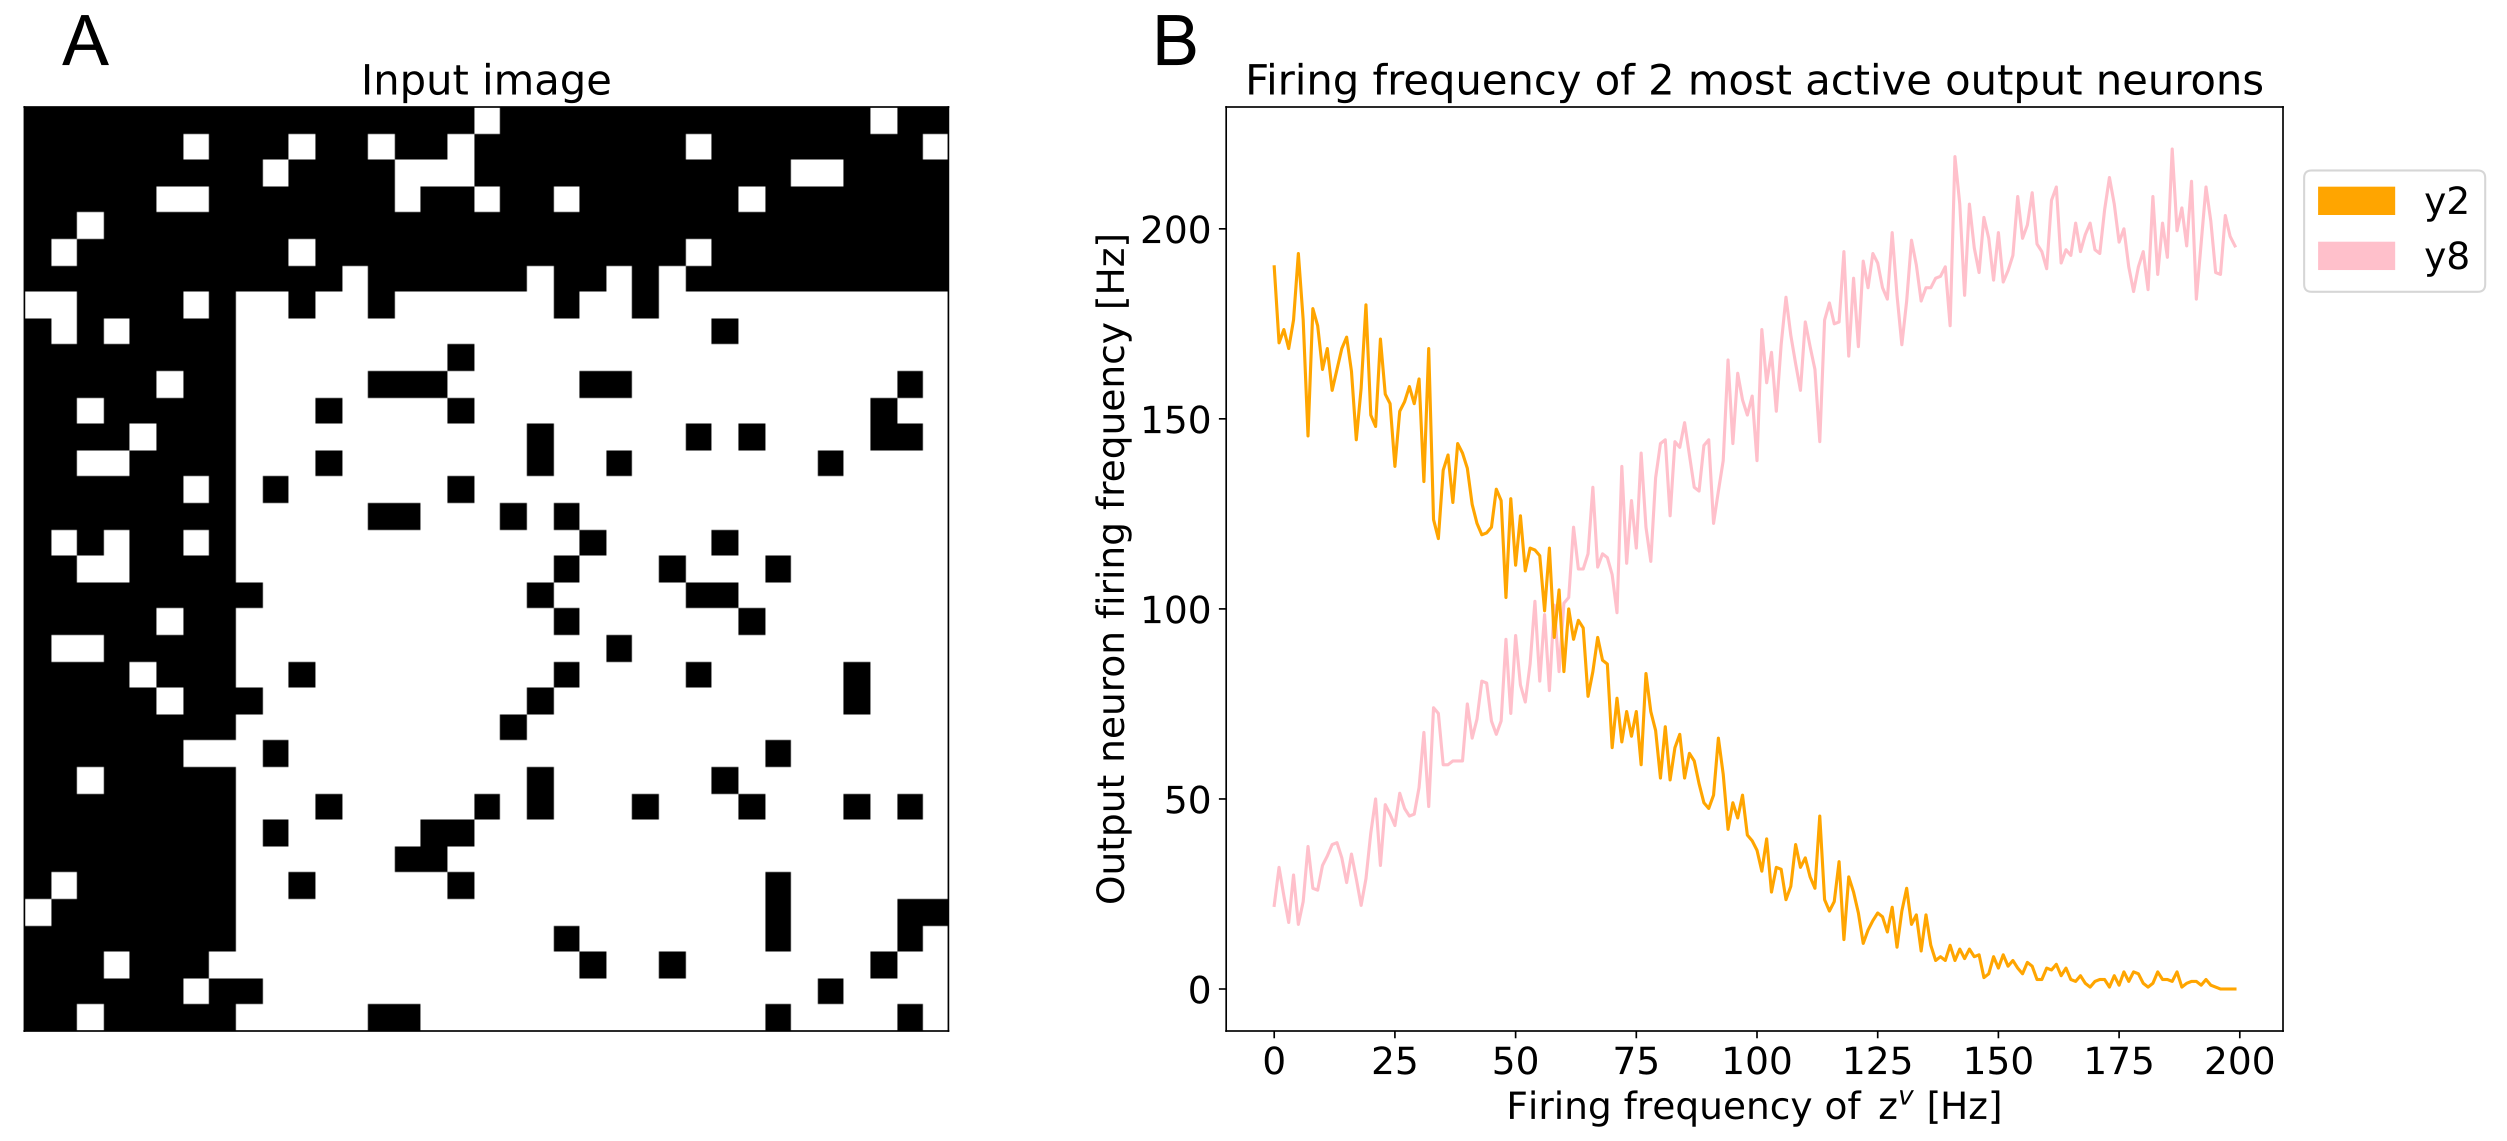
\includegraphics[width=\linewidth]{figures/horvertAdaptiveInh/YFrequency_prior.png}
  \caption{\textbf{Cross image with varying prior neuron activity.} \textbf{A} Validation cross image. \textbf{B} Firing frequency of the 2 most active output neurons depending on the firing frequency of $z^v$. The output neuron firing frequencies were averaged over 10 runs to smooth the graphs.}
  \label{fig:horvertAdaptiveInhibitionVariablePriorResults}
\end{figure}





























%%%
%%%
%%%
%%%
% unused exp, kept for looking up stuff

\iffalse
\section{Experiment 2: Horizontal and vertical bars}
\label{section:horvert}

 \subsection{Introduction}

For this experiment the impact of a neuron layer that encodes a-priori information should be analysed.

\subsection{Methods}

\paragraph{Input data}
29 x 29 black and white images with either horizontal or vertical oriented bars on them were used, as it was more straightforward to express a-priori information. The orientation of the training images was chosen randomly via a uniform distribution. Also the positions of the bars in the images were uniformly distributed. The rest of the image generation process is analogous to experiment 1, except no circular mask was used. Examples of the input data can be seen in Figure \ref{fig:horvertImages}. To show the value of the a-priori information validation images with two bars forming a cross were also generated, seen in Figure \ref{fig:horvertTrainingCrossImage}. When shown to the network in the validation process the prior neurons were given the information that a cross is either in horizontal or vertical orientation.

\begin{figure}
  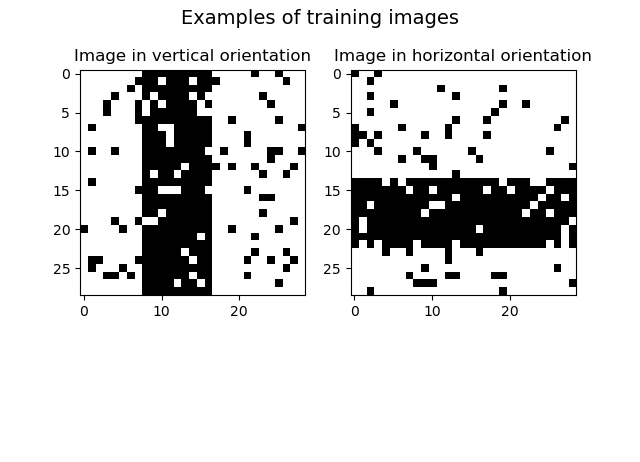
\includegraphics[width=\linewidth]{figures/horvert/horvertTrainingImages.png}
  \caption{Training images generated for experiment 2. One image of each possible orientation at a random position.}
\end{figure}

\begin{figure}
  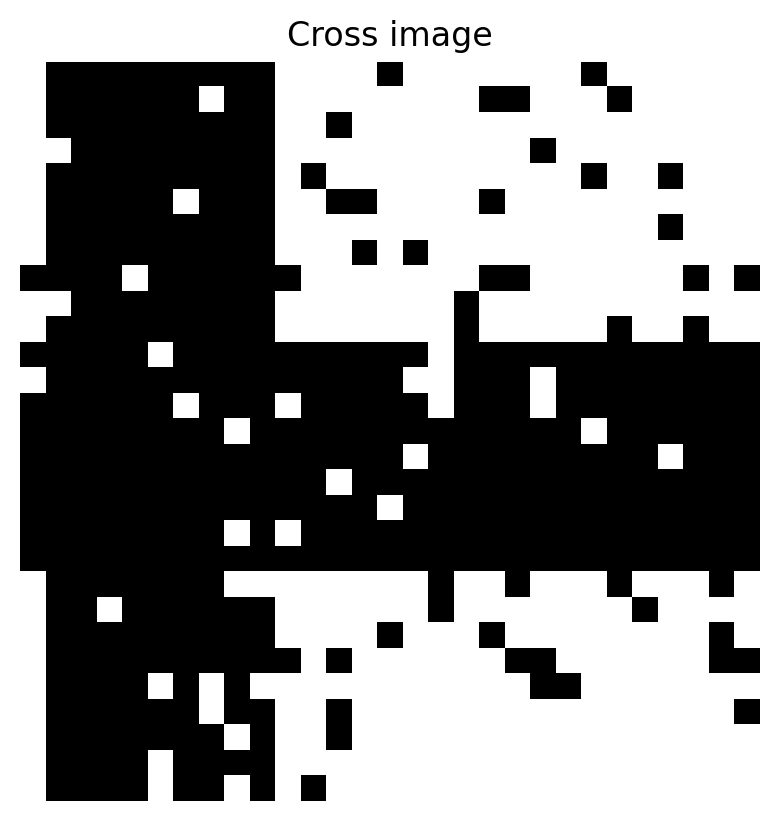
\includegraphics[width=0.6\linewidth]{figures/horvert/horvertTrainingCrossImage.png}
  \caption{Generated cross image which can represent either horizontal or vertical orientation.}
  \label{fig:horvertTrainingCrossImage}
\end{figure}


\paragraph{Network architecture}

This experiment used a expanded version of the network used in experiment 1. An additional layer of prior neurons $z_1,z_2$ was added. Whenever an image was oriented vertically $z_1$ was active and $z_2$ was inactive. For horizontal orientations $z_2$ was active and $z_1$ was inactive. Prior neurons in an active state had a firing frequency of 50 Hz and fired with 0 Hz when inactive.

\paragraph{Neuron model}
The input and output neurons functioned the same way as in the previous experiment. The prior neurons fire according to a poisson process with their firing rate. Each prior neuron $Z_l$ is connected to every output neuron $Y_k$ and thus has weights $w_{kl}$ that were learned by the network. 

\paragraph{Parameters}
As the number of input neurons and the average number of black pixels in an input image stayed roughly the same in this experiment, the same parameters $c=  20$ and $\lambda = 10^{-3}$ could be used.

%% START
%% this block was copied to Theoretical Background, cut this accordingly
%% Zfactor does not exist, remove!!!
 However as there are only two prior neurons, a way to amplify their produced signals was needed, otherwise their impact on the membrane potential of the output neurons would not be distinctive enough. So the EPSPs $z_l(t)$ were multiplied by the factor $Z_{factor}$. This factor was determined via grid search. The additional prior layer resulted in an expanded version of the membrane potential $u_k(t)$

\begin{equation}
\label{eqn:ukHorvert}
u_k(t) = \sum_{i=1}^n w_{ki} \cdot x_i(t) + \sum_{j=1}^n w_{kj} \cdot Z_{factor} \cdot z_j(t).
\end{equation}

%% END

\subsection{Results} 

The following values for $Z_{factor} $ were tried with $c = 20$ and $\lambda = 10^{-3}$:
\begin{itemize}
  \item $Z_{factor} = 3$
  \item $Z_{factor} = 5$
  \item $Z_{factor} = 7$  
  \item $Z_{factor} = 10$ 
  \item $Z_{factor} = 20$
\end{itemize}

For $Z_{factor} = 10$ and $20$ the prior neurons impacted the learning progress negatively and let single prior neurons respond to too much area. An example of this can be seen in Figure \ref{fig:horvert_c20_3_Zfactor20_horizontalLines}

\begin{figure}
  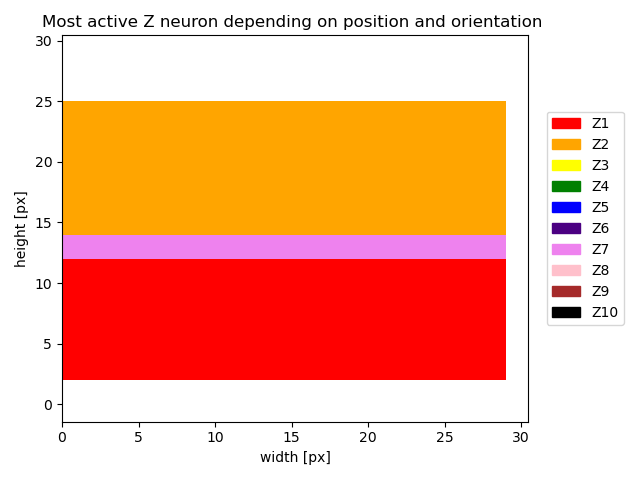
\includegraphics[width=\linewidth]{figures/horvert/horvert_c20_3_Zfactor20_horizontalLines.png}
  \caption{Most active output neuron for horizontal orientation and position on the y-axis of the training image during the training process. $c = 20, \lambda = 10^{-3}, Z_{factor} = 20$}
  \label{fig:horvert_c20_3_Zfactor20_horizontalLines}
\end{figure}


The best results were achieved with $Z_{factor} = 5$. When looking at the training progress in Figure \ref{fig:horvert_c20_3_Zfactor5_averageZ} it can be seen that the training accuracy is higher compared to experiment 1. This is due to the added a-priori information and the fact that less of each bar in an image is overlapping with multiple areas of output neurons. The network activity at the end of the training process can be seen in Figure \ref{fig:horvertLastSpikes}. In Figures \ref{fig:horvert_c20_3_Zfactor5_horizontalLines} and \ref{fig:horvert_c20_3_Zfactor5_verticalLines} the most active output neuron of the trained network is plotted for horizontal bars in every position and in the second plot for vertical bars in every position. Every one of the ten output neurons responds primarily to one coherent area in one orientation. The values of the learned prior weights $w_{kl}$ were plotted in Figures \ref{fig:wkl1} and \ref{fig:wkl2}. In these figures, in combination with Figures \ref{fig:horvert_c20_3_Zfactor5_horizontalLines} and \ref{fig:horvert_c20_3_Zfactor5_verticalLines}, can be seen that each prior neuron specialized on one orientation.

\begin{figure}
  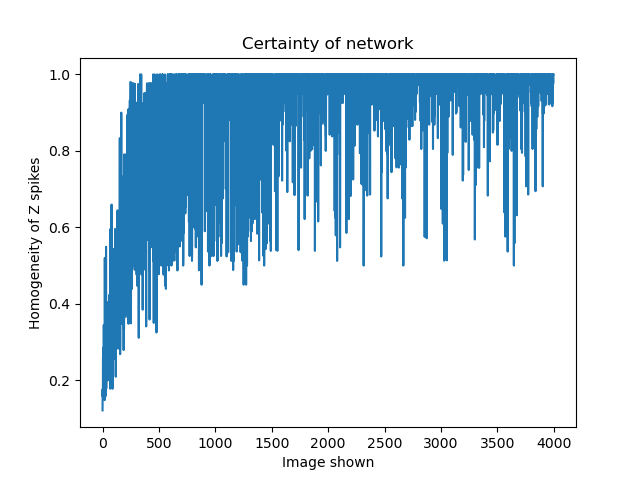
\includegraphics[width=\linewidth]{figures/horvert/horvert_c20_3_Zfactor5_averageZ.png}
  \caption{Proportion (accuracy) of most active output neuron  to activity of all other output neurons during the presentation duration of each training image. $c = 20, \lambda = 10^{-3}, Z_{factor} = 5$}
  \label{fig:horvert_c20_3_Zfactor5_averageZ}
\end{figure}

\begin{figure}
  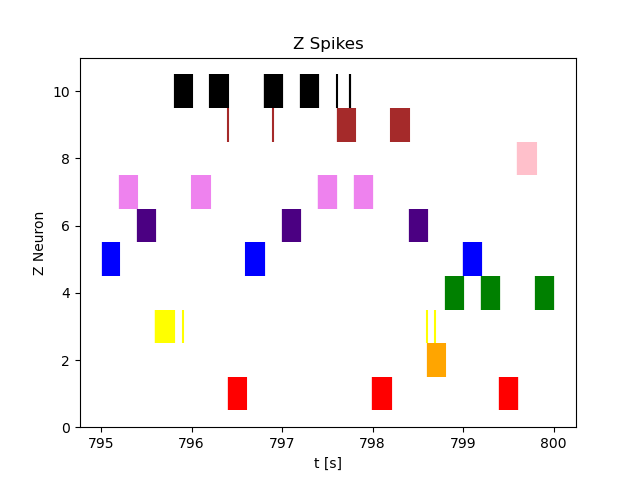
\includegraphics[width=\linewidth]{figures/horvert/horvert_c20_3_Zfactor5_1000LastZSpikes.png}
  \caption{Last 1000 output neuron spikes, $c = 20, \lambda = 10^{-3}$, $Z_{factor} = 5$}
  \label{fig:horvertLastSpikes}
\end{figure}

\begin{figure}
  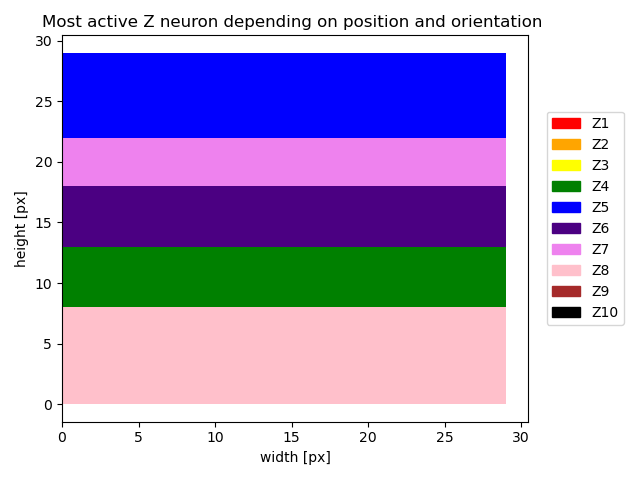
\includegraphics[width=\linewidth]{figures/horvert/horvert_c20_3_Zfactor5_horizontalLines.png}
  \caption{Most active output neuron for images of horizontal orientation and position on the x-axis of during the validation process. $c = 20, \lambda = 10^{-3}, Z_{factor} = 5$}
  \label{fig:horvert_c20_3_Zfactor5_horizontalLines}
\end{figure}

\begin{figure}
  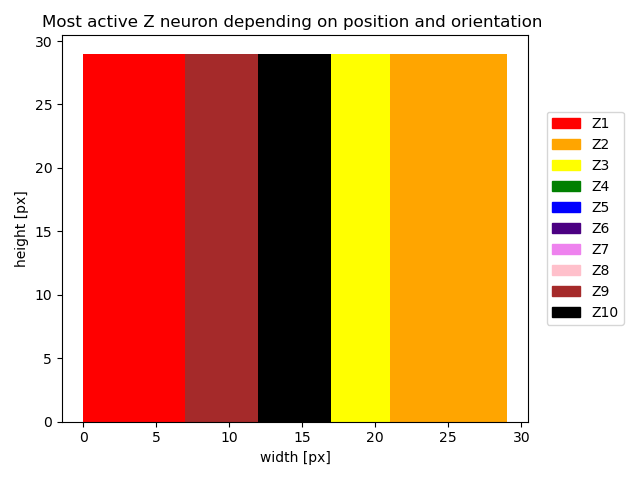
\includegraphics[width=\linewidth]{figures/horvert/horvert_c20_3_Zfactor5_verticalLines.png}
  \caption{Most active output neuron for images of vertical orientation and position on the x-axis of during the validation process. $c = 20, \lambda = 10^{-3}, Z_{factor} = 5$}
  \label{fig:horvert_c20_3_Zfactor5_verticalLines}
\end{figure}

\begin{figure}
  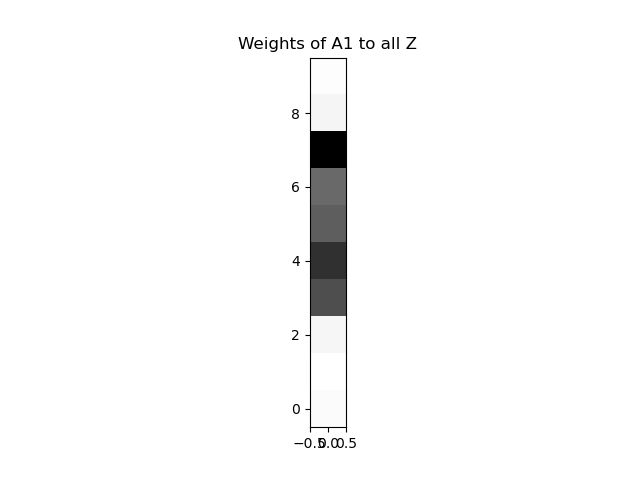
\includegraphics[width=\linewidth]{figures/horvert/horvert_c20_3_Zfactor5_priorWeight1.png}
  \caption{Values of $w_k1$, darker color means higher value. $c = 20, \lambda = 10^{-3}, Z_{factor} = 5$}
  \label{fig:wkl1}
\end{figure}

\begin{figure}
  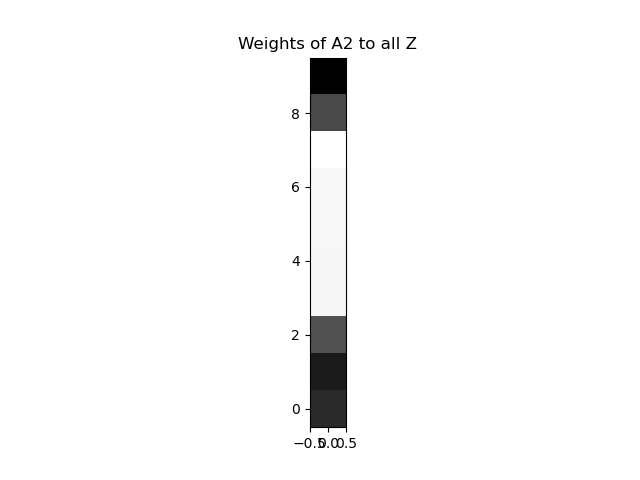
\includegraphics[width=\linewidth]{figures/horvert/horvert_c20_3_Zfactor5_priorWeight2.png}
  \caption{Values of $w_k2$, darker color means higher value. $c = 20, \lambda = 10^{-3}, Z_{factor} = 5$}
  \label{fig:wkl2}
\end{figure}

During the validation of all possible horizontal bar images the output spike activity was recorded and how many distinct output neurons were spiking during each image presentation period. For the parts where the 7 pixels high bar in the image did not overlap the areas of two output neurons only one output neuron was active. Only in the border areas there were two output neurons active. This can be seen in Figures \ref{fig:horvert_c20_3_Zfactor5_horizontalDistinctZ} and \ref{fig:horvert_c20_3_Zfactor5_horizontalZSpikes}. Compared to experiment 1 the activity is more homogeneous as each bar can only be in at most the area of four output neurons, when two of these areas are reinforced by the prior neurons.

\begin{figure}
  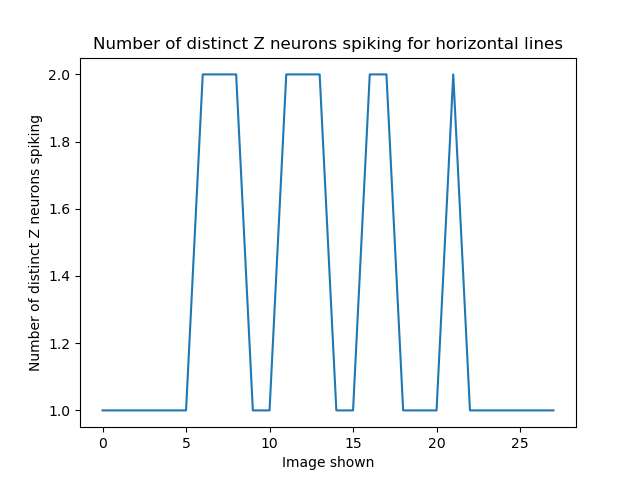
\includegraphics[width=\linewidth]{figures/horvert/horvert_c20_3_Zfactor5_horizontalDistinctZ.png}
  \caption{Distinct output neurons spiking during the presentation of all possible horizontal oriented validation images, $c = 20, \lambda = 10^{-3}$, $Z_{factor} = 5$}
  \label{fig:horvert_c20_3_Zfactor5_horizontalDistinctZ}
\end{figure}
\begin{figure}
  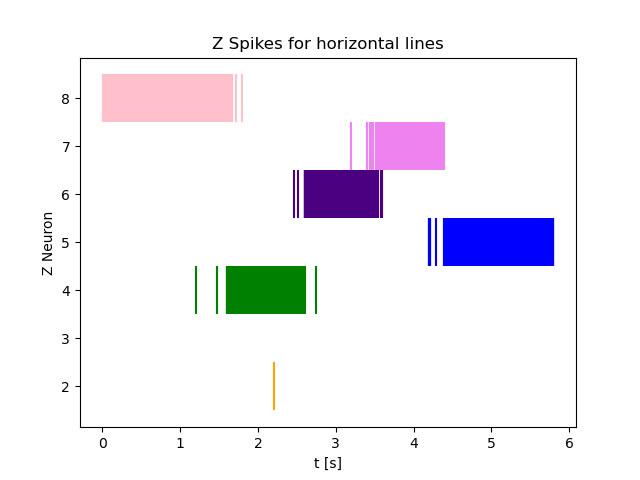
\includegraphics[width=\linewidth]{figures/horvert/horvert_c20_3_Zfactor5_horizontalZSpikes.png}
  \caption{Output neuron spikes during the presentation of all possible horizontal oriented validation images, $c = 20, \lambda = 10^{-3}$, $Z_{factor} = 5$}
  \label{fig:horvert_c20_3_Zfactor5_horizontalZSpikes}
\end{figure}


To show the impact of the prior neurons an image with two bars on it forming a cross (Figure \ref{fig:horvertValidationCross}) was generated and $z_2$ was set active indicating that the orientation is supposed to be horizontal. This resulted in the spiking pattern seen in Figure \ref{fig:horvert_c20_3_Zfactor5_crossZSpikes}. In it $Y_1$ is more active than $Y_9$ due to the influence of the prior neuron $Z_2$.

\begin{figure}
  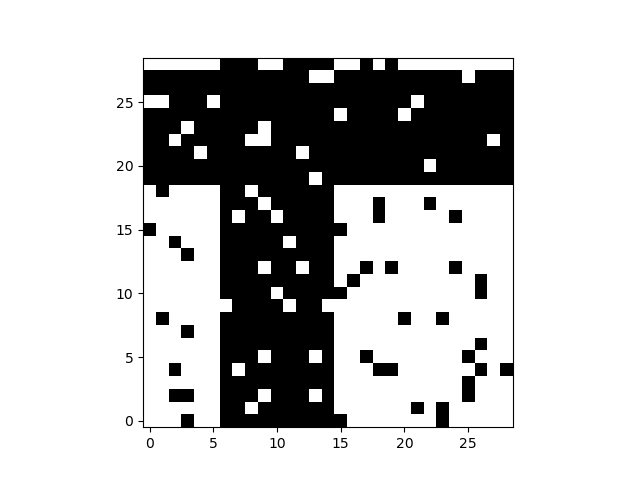
\includegraphics[width=\linewidth]{figures/horvert/horvert_c20_3_Zfactor5_validationCross.png}
  \caption{Generated validation cross image, with orientation defined as horizontal. $c = 20, \lambda = 10^{-3}, Z_{factor} = 5$}
  \label{fig:horvertValidationCross}
\end{figure}

\begin{figure}
  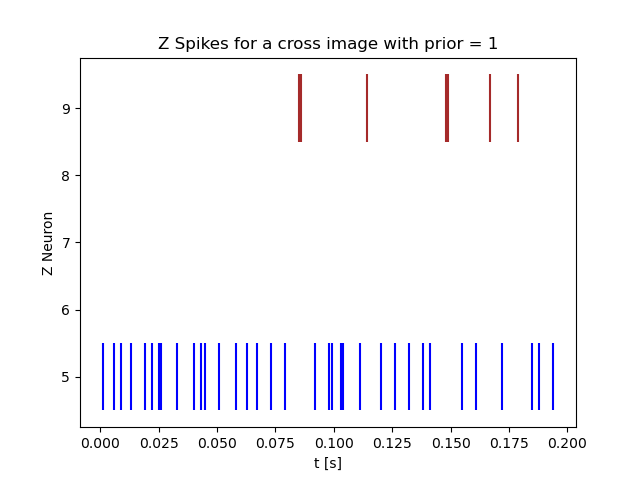
\includegraphics[width=\linewidth]{figures/horvert/horvert_c20_3_Zfactor5_crossZSpikes.png}
  \caption{Output spikes during the presentation of the validation cross image. $c = 20, \lambda = 10^{-3}, Z_{factor} = 5$}
  \label{fig:horvert_c20_3_Zfactor5_crossZSpikes}
\end{figure}

\fi
\section{Experiment 2: Mathematical analysis of the network with 1-D images}
\label{section:1D}

\subsection{Introduction}

The purpose of this experiment was to analyse a smaller network and provide a definitive way to verify the performance of the simulation. Furthermore, the weights were not learned as in the previous experiment, but rather determined analytically. This was done to experimentally prove the relation given by \citet{nessler} that the weights stochastically converge toward the conditional probability that a presynaptic neuron fired shortly before the postsynaptic neuron.
First the network was scaled down to be one-dimensional with 18 input neurons, four prior neurons and four output neurons, making it easier to analyse. The weights were determined by utilizing the logarithmic connection between them and the corresponding conditional probabilities, as given by Equation \ref{eqn:weightProbLink}. The conditional probabilities of the input and output neurons of the network  were calculated and then used to determine the posterior probability of the network. After the simulation of the network the distribution of the output spikes was used to calculate the posterior probability. The posterior probabilities of both the mathematical analysis and the simulation were compared. By varying three network hyperparameters it was tuned to approximate the analytical solution as closely as possible.

\subsection{Methods}

\paragraph{Input data}
The input image consisted of nine pixels in a horizontal line. Within those nine pixels, going from position 0 to 8, four output classes could be represented. Each output class had of three pixels next to each other. This resulted in each output class overlapping its neighbour classes by one pixel. Thus the centers of the output classes were at position 1, 3, 5 and 7.
 
\paragraph{Network architecture}
Compared to the architecture of the previous experiment only the amount of neurons was changed. As there have to be 2 input neurons for each pixel, one neuron being active if the pixel is white and one if the pixel is black, the network had 18 input neurons. Furthermore four prior neurons were implemented, of which only one is being active for one of the output classes at a time. Lastly the network had four output neurons.

\paragraph{Mathematical Analysis}
The posterior probability of the network was calculated by using Equation \ref{eqn:pYvorausgesetztXUndZ}.
$P(X=x|Y=k)$ and $P(Y=k|Z=j)$ were derived corresponding to the paradigm of the experiment.
 The calculation of $P(X=x|Y=k)$ was split into two parts. First the contribution of the active input neurons was calculated by determining the matrix $P^{X|Y}$. This matrix is of size 4 x 9 and contains the conditional probabilities of each input neuron $y_k$ being active, given that an output neuron $x_i$ is active. These probabilities were calculated by determining which input neurons are active depending on the output class and which input neurons are inactive, as dictated by the network architecture. Furthermore, the noise that was applied to the input neurons had to be taken into account. For input neurons belonging to the output class the conditional probability was determined as 1 and lowered by the noise level, while for the input neurons outside of the 3-wide pixel block belonging to the output class it was determined as 0 and raised by the noise level. According to this $P^{X|Y}$ is given by
\begin{equation}
\label{eqn:PXvorausgesetztYIf}
P_{k,i}^{X|Y} = \begin{dcases*} 1 - $noise level$ & if $x_i$ is in the active area of $y_k$, \\
0 + $noise level$ & \text{if $x_i$ is not in the active area of $ y_k $ } \end{dcases*}.\end{equation}
  After calculating all entries of $P^{X|Y}$ its rows were multiplied with the input image vector
\begin{equation}
\label{eqn:p1XvorausgesetztYMalX}
P_1(X = x|Y = k) = P^{X|Y}_{k,*} \cdot x
\end{equation}
resulting in a conditional probability for each output class depending on the input vector. The input vector was given with entries of 1 for active pixels and with entries of 0 for inactive pixels.
Next to include the contribution of the input neurons that are spiking when a pixel is inactive the conditional probability of the input neurons that are active for the entries where $x_i = 0$ had to be calculated. To achieve this complementary conditional probability at first $P^{X|Y}$ was subtracted from one. To include the correct conditional probabilities for the complementary case the input image vector x was then also subtracted from one. $1 - P^{X|Y}$ and $1 - x$ were multiplied to yield
\begin{equation}
\label{eqn:p2minusXvorausgesetztYMalX}
P_2(X = x|Y = k) = (1 - P^{X|Y}_{k,*}) \cdot (1 - x).
\end{equation}
The results of both calculations were then multiplied element-wise to yield
\begin{equation}
\label{eqn:pXvorausgesetztY}
P(X = x|Y = k) = P_1(X = x|Y = k) \odot P_2(X = x|Y = k).
\end{equation}
$P(Y=k|Z=j)$ was determined by first calculating the matrix $P^{Y|Z}$. It has a dimension of 4 x 4 and contains the conditional probabilities for the output neuron $y_k$, given the prior neuron $z_j$ being active. For each output class there exists one corresponding prior neuron. As there can never be more than one active prior neuron at a time $P^{Y|Z}$ is given by
\begin{equation}
\label{eqn:PYvorausgesetztZIf}
P_{k,j}^{Y|Z} = \begin{dcases*} 1 - $noise level$ & if $i = j$, \\
0 +  \frac{1}{3}  $noise level$ & \text{if $i \neq j$. } \end{dcases*}\end{equation} 
$P(Y=k|Z=j)$ was then obtained by
\begin{equation}
\label{eqn:pYvorausgesetztZ}
P(Y=k|Z=j) = P^{Y|Z} \cdot z
\end{equation}
where z is given by a 4 x 1 one-hot encoded vector of the prior.

\paragraph{Simulation}
The input weights for the simulation were calculated as two separate sets. First weights $w^{I1}$ for the input neurons that are active for active input pixels were determined by 
\begin{equation}
\label{eqn:1DWeights}
w^{I1} = \ln(P^{X|Y}).
\end{equation}
Second complementary input weights $w^{I2}$ were calculated for  input neurons representing non active input pixels with
\begin{equation}
\label{eqn:1DWeightsComplementary}
w^{I2} = \ln(1 - P^{X|Y}).
\end{equation} 
The prior weights $w^P$ were derived by 
\begin{equation}
\label{eqn:1DWeightsPrior}
w^P = \ln(P^{Y|Z}).
\end{equation}

The network was simulated for six different input images for each hyperparameter set. These six images were hand-picked to include specific edge cases and to allow comparability of the results of different hyperparameter sets. After the image presentation period of each input image the numbers of output spikes of each class were counted and their proportions were calculated to yield the posterior $P_{simulation}(Y = k|X, Z)$. The Kullback-Leibler divergence was chosen to compare the divergence of the analytic and the simulated posteriors of the network. This metric indicates how much two probability distributions diverge from each other. The goal of the hyperparameter search of the simulation was to minimize the Kullback-Leibler divergence. After showing an output image to the network the Kullback-Leibler divergence was calculated as
\begin{equation}
\begin{split}
\label{eqn:KLDivergence}
D_{KL}(P_{analysis}(Y = k|X, Z)||P_{simulation}(Y = k|X, Z)) = \\ \sum_{k=1}^K P_{analysis}(Y = k|X, Z) \cdot \ln( \frac{P_{analysis}(Y = k|X, Z)}{P_{simulation}(Y = k|X, Z)})
\end{split}
\end{equation}
where K is the number of output neurons and $P_{analysis}(Y = k|X, Z)$ and $P_{simulation}(Y = k|X, Z)$ are the posteriors of the network, late called "analysis output probabilities" and "simulation output probabilities" in plots. The six resulting Kullback-Leibler divergences for each hyperparameter set were then averaged to create a single metric by which the performance of the different hyperparameter sets was compared. The three hyperparameters input firing rate $f_{input}$, prior firing rate $f_{prior}$ and the membrane constant $\tau_{decay}$ were varied to inspect their influence on the result, as well as to approximate the analytical solution as closely as possible. Each input image was presented to the network for 20 seconds to reduce the variance between runs. Furthermore each simulation was repeated 20 times with the same hyperparameter set to obtain the mean and standard deviation of the simulation output probabilities and of the Kullback-Leibler divergence.

\subsection{Results}

\paragraph{Analytic Results}

First the matrix $P^{X|Y}$ was calculated using Equation \ref{eqn:PXvorausgesetztYIf} 
\begin{equation}
\label{eqn:pXvorausgesetztYResult}
P^{X|Y} = \begin{bmatrix}
0.9 & 0.9 & 0.9 & 0.1 & 0.1 & 0.1 & 0.1 & 0.1 & 0.1\\
0.1 & 0.1 & 0.9 & 0.9 & 0.9 & 0.1 & 0.1 & 0.1 & 0.1\\
0.1 & 0.1 & 0.1 & 0.1 & 0.9 & 0.9 & 0.9 & 0.1 & 0.1\\
0.1 & 0.1 & 0.1 & 0.1 & 0.1 & 0.1 & 0.9 & 0.9 & 0.9\\
\end{bmatrix}.
\end{equation}
Next the matrix $P^{Y|Z}$ was calculated using Equation \ref{eqn:PYvorausgesetztZIf} 
\begin{equation}
\label{eqn:pYvorausgesetztZResult}
P^{Y|Z} = \begin{bmatrix}
0.9 & 0.0333 & 0.0333 & 0.0333\\
0.0333 & 0.9 & 0.0333 & 0.0333\\
0.0333 & 0.0333 & 0.9 & 0.0333\\
0.0333 & 0.0333 & 0.0333 & 0.9\\
\end{bmatrix}.
\end{equation} 
For each input image these two matrices were multiplied with the input vector and prior vector as described Equations \ref{eqn:p1XvorausgesetztYMalX}, \ref{eqn:p2minusXvorausgesetztYMalX},  \ref{eqn:pXvorausgesetztY} and \ref{eqn:pYvorausgesetztZ} to yield $P(X = x|Y = i)$ and $P(Y=i|Z=j)$. Using \ref{eqn:pYvorausgesetztXUndZ}  finally yielded the analytical $P(Y = i|X = x, Z = j)$.

\paragraph{Simulation results with prior disabled}
To simplify the hyperparameter fitting process the network was at first simulated with inactive prior neurons. Only after determining the best values for $f_{input}$ and $\tau_{decay}$ the prior neurons were reactivated and $f_{prior}$ was fitted. The values 0.015 seconds and 0.004 seconds for $\tau_{decay}$ were used for the simulation and compared. For each of these values an optimal value for $f_{input}$ was found by looking for the value that yielded the smallest Kullback-Leibler divergence.

\subparagraph{$\tau_{decay} = 0.015 seconds$, $f_{prior} = 0 Hz$}
Values for $f_{input}$ between 10 and 110 Hz in steps of 10 Hz were simulated. After identifying the input firing rate with the smallest Kullback-Leibler divergence the network was simulated again for $f_{input}$ values $\pm$ 10 Hz in steps of 2 Hz. The result of this search can be seen in Figure \ref{fig:1D_KLD_fPrior0_tau15}. This process yielded the best input firing rate of 42 Hz. The results of this hyperparameter combination can be seen in Figure \ref{fig:1D_42_0_15}. In this figure six different input images can be seen in A. The active pixels are shown in black. In B the posterior probabilities of the mathematical analysis are given by the red bars and the posterior probabilities of the simulation are given by the blue bars. Each simulation output probability has its standard deviation marked by a black bar. At the bottom the value of the Kullback-Leibler divergence is given, with its standard deviation. The exact numeric probabilities are given in Table \ref{tab:1D_42_0_15}.

\begin{figure}
  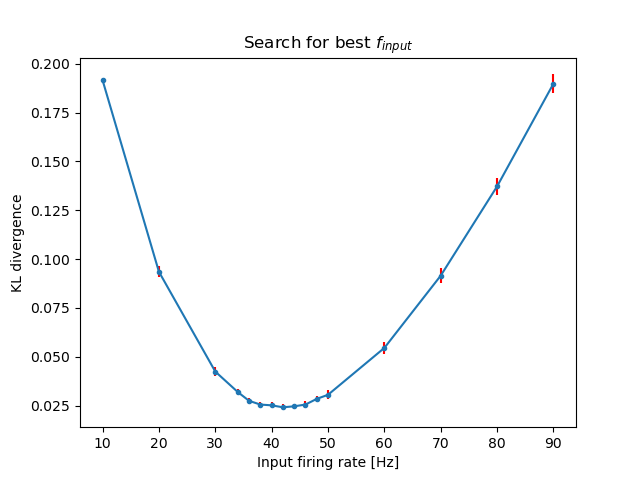
\includegraphics[width=\linewidth]{figures/1D/KLDvsfInput_fPrior0tau15.png}
  \caption{\textbf{KL divergence for different $f_{input}$ values. } Hyperparameters: $f_{prior} = 0 Hz, \tau_{decay} = 15 ms$}
  \label{fig:1D_KLD_fPrior0_tau15}
\end{figure}

\begin{figure}
  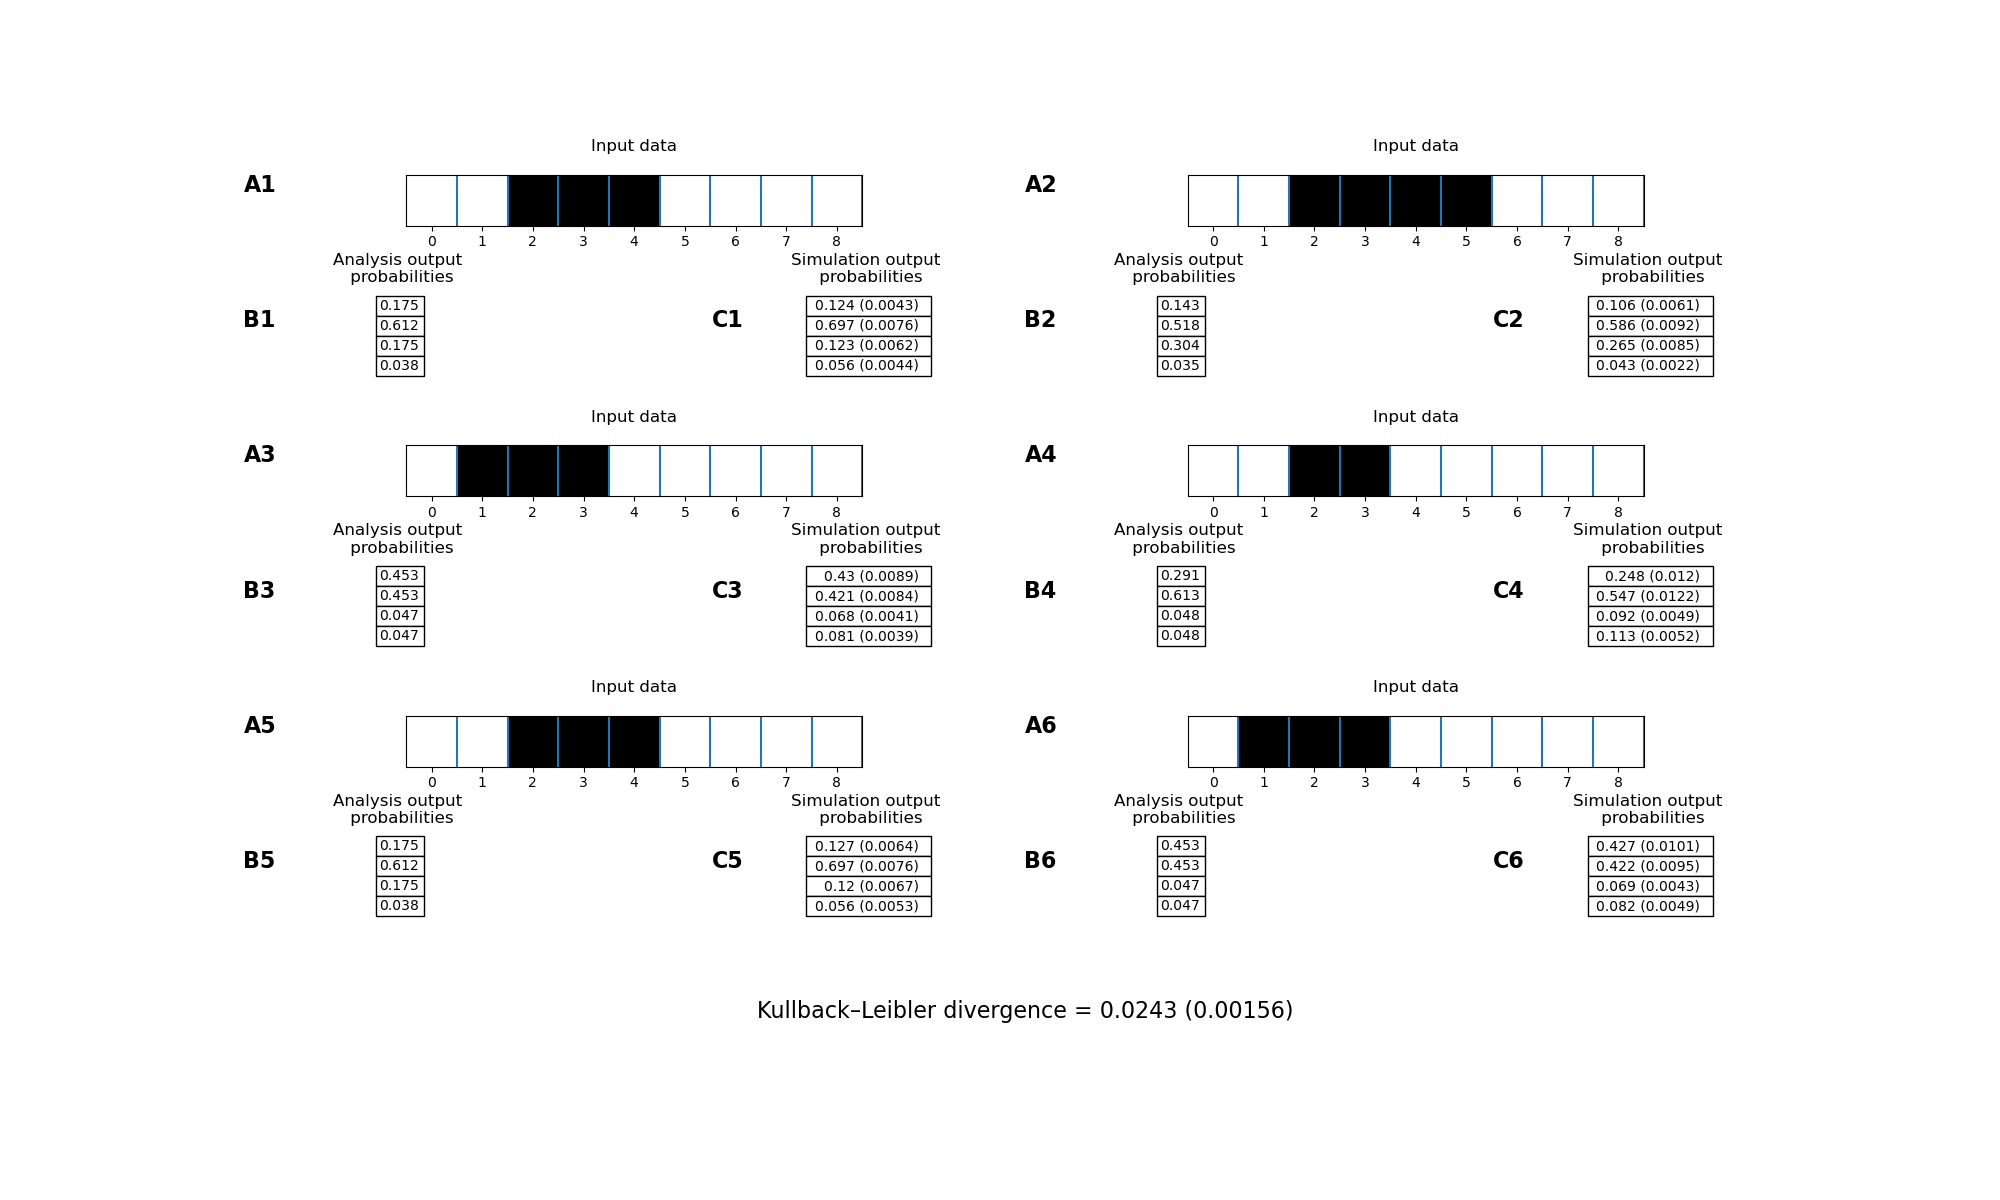
\includegraphics[width=\linewidth]{figures/1D/1D_42_0_15.png}
  \caption{\textbf{Analysis and simulation result. } Hyperparameters: $f_{input} = 42 Hz, f_{prior} = 0 Hz, \tau_{decay} = 15 ms$ \textbf{A} Input images with 9 x 1 pixels. \textbf{B} Analytically calculated posterior probabilities and simulated posterior probabilities. The standard deviations are given by the black bars.}
  \label{fig:1D_42_0_15}
\end{figure}

\begin{table}[]
\label{tab:1D_42_0_15}
\small
\tabcolsep=0.11cm
\begin{tabular}{|c|cc|cc|}
\hline
                       & \multicolumn{2}{c|}{Image 1}                       & \multicolumn{2}{c|}{Image 2}                       \\ \hline
                       & \multicolumn{1}{c|}{Analysis} & Simulation         & \multicolumn{1}{c|}{Analysis} & Simulation         \\ \hline
$y_0$                  & \multicolumn{1}{c|}{0.175}    & 0.124 $\pm$ 0.0061 & \multicolumn{1}{c|}{0.143}    & 0.104 $\pm$ 0.0059 \\ \hline
$y_1$                  & \multicolumn{1}{c|}{0.612}    & 0.699 $\pm$ 0.0093 & \multicolumn{1}{c|}{0.518}    & 0.587 $\pm$ 0.0090 \\ \hline
$y_2$                  & \multicolumn{1}{c|}{0.175}    & 0.121 $\pm$ 0.0058 & \multicolumn{1}{c|}{0.304}    & 0.266 $\pm$ 0.0067 \\ \hline
$y_3$                  & \multicolumn{1}{c|}{0.038}    & 0.056 $\pm$ 0.0033 & \multicolumn{1}{c|}{0.035}    & 0.043 $\pm$ 0.0025 \\ \hline
                       & \multicolumn{2}{c|}{Image 3}                       & \multicolumn{2}{c|}{Image 4}                       \\ \hline
$y_0$                  & \multicolumn{1}{c|}{0.453}    & 0.430 $\pm$ 0.0089 & \multicolumn{1}{c|}{0.291}    & 0.245 $\pm$ 0.0065 \\ \hline
$y_1$                  & \multicolumn{1}{c|}{0.453}    & 0.421 $\pm$ 0.0073 & \multicolumn{1}{c|}{0.613}    & 0.553 $\pm$ 0.0072 \\ \hline
$y_2$                  & \multicolumn{1}{c|}{0.047}    & 0.070 $\pm$ 0.0045 & \multicolumn{1}{c|}{0.048}    & 0.090 $\pm$ 0.0045 \\ \hline
$y_3$                  & \multicolumn{1}{c|}{0.047}    & 0.080 $\pm$ 0.0042 & \multicolumn{1}{c|}{0.048}    & 0.111 $\pm$ 0.0053 \\ \hline
						& \multicolumn{2}{c|}{Image 5}                       & \multicolumn{2}{c|}{Image 6}                       \\ \hline
$y_0$                  & \multicolumn{1}{c|}{0.175}    & 0.124 $\pm$ 0.0046 & \multicolumn{1}{c|}{0.453}    & 0.428 $\pm$ 0.0116 \\ \hline
$y_1$                  & \multicolumn{1}{c|}{0.612}    & 0.697 $\pm$ 0.0069 & \multicolumn{1}{c|}{0.453}    & 0.421 $\pm$ 0.0111 \\ \hline
$y_2$                  & \multicolumn{1}{c|}{0.175}    & 0.123 $\pm$ 0.0050 & \multicolumn{1}{c|}{0.047}    & 0.070 $\pm$ 0.0034 \\ \hline
$y_3$                  & \multicolumn{1}{c|}{0.038}    & 0.056 $\pm$ 0.0043 & \multicolumn{1}{c|}{0.047}    & 0.081 $\pm$ 0.0047 \\ \hline
\end{tabular}
\caption{\textbf{Analysis and simulation output probabilities. } Hyperparameters: $f_{input} = 42 Hz, f_{prior} = 0 Hz, \tau_{decay} = 15 ms$}
\end{table}

When $f_{input}$ was 70 Hz the results of the analysis and the simulation differed more as can be seen in Figure \ref{fig:1D_70_0_15} and Table \ref{tab:1D_70_0_15}.

\begin{figure}
  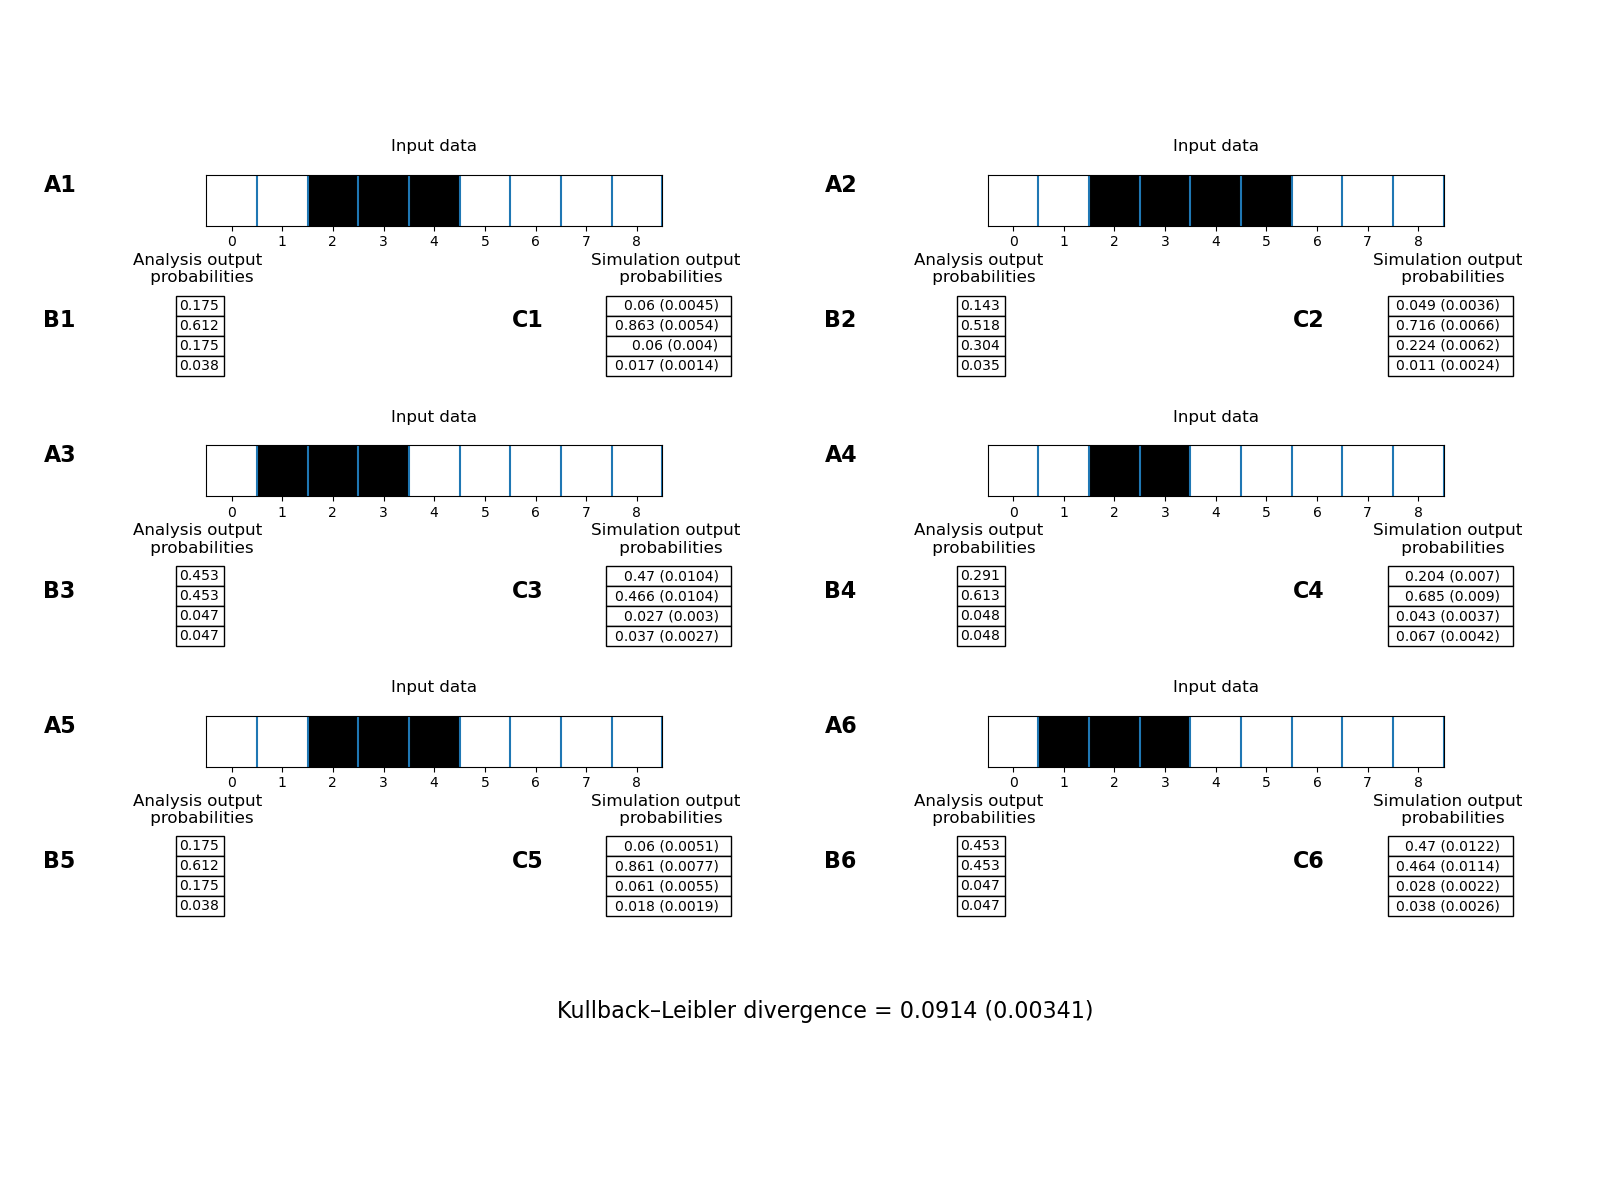
\includegraphics[width=\linewidth]{figures/1D/1D_70_0_15.png}
    \caption{\textbf{Analysis and simulation result. } Hyperparameters: $f_{input} = 70 Hz, f_{prior} = 0 Hz, \tau_{decay} = 15 ms$ \textbf{A} Input images with 9 x 1 pixels. \textbf{B} Analytically calculated posterior probabilities and simulated posterior probabilities. The standard deviations are given by the black bars.}
  \label{fig:1D_70_0_15}
\end{figure}

\begin{table}[]
\label{tab:1D_70_0_15}
\small
\tabcolsep=0.11cm
\begin{tabular}{|c|cc|cc|}
\hline
                       & \multicolumn{2}{c|}{Image 1}                       & \multicolumn{2}{c|}{Image 2}                       \\ \hline
                       & \multicolumn{1}{c|}{Analysis} & Simulation         & \multicolumn{1}{c|}{Analysis} & Simulation         \\ \hline
$y_0$                  & \multicolumn{1}{c|}{0.175}    & 0.061 $\pm$ 0.0038 & \multicolumn{1}{c|}{0.143}    & 0.049 $\pm$ 0.0027 \\ \hline
$y_1$                  & \multicolumn{1}{c|}{0.612}    & 0.861 $\pm$ 0.0065 & \multicolumn{1}{c|}{0.518}    & 0.715 $\pm$ 0.0083 \\ \hline
$y_2$                  & \multicolumn{1}{c|}{0.175}    & 0.061 $\pm$ 0.0041 & \multicolumn{1}{c|}{0.304}    & 0.226 $\pm$ 0.0070 \\ \hline
$y_3$                  & \multicolumn{1}{c|}{0.038}    & 0.017 $\pm$ 0.0016 & \multicolumn{1}{c|}{0.035}    & 0.011 $\pm$ 0.0017 \\ \hline
                       & \multicolumn{2}{c|}{Image 3}                       & \multicolumn{2}{c|}{Image 4}                       \\ \hline
$y_0$                  & \multicolumn{1}{c|}{0.453}    & 0.472 $\pm$ 0.0100 & \multicolumn{1}{c|}{0.291}    & 0.207 $\pm$ 0.0067 \\ \hline
$y_1$                  & \multicolumn{1}{c|}{0.453}    & 0.464 $\pm$ 0.0101 & \multicolumn{1}{c|}{0.613}    & 0.685 $\pm$ 0.0080 \\ \hline
$y_2$                  & \multicolumn{1}{c|}{0.047}    & 0.027 $\pm$ 0.0027 & \multicolumn{1}{c|}{0.048}    & 0.043 $\pm$ 0.0037 \\ \hline
$y_3$                  & \multicolumn{1}{c|}{0.047}    & 0.037 $\pm$ 0.0032 & \multicolumn{1}{c|}{0.048}    & 0.065 $\pm$ 0.0042 \\ \hline
						& \multicolumn{2}{c|}{Image 5}                       & \multicolumn{2}{c|}{Image 6}                       \\ \hline
$y_0$                  & \multicolumn{1}{c|}{0.175}    & 0.061 $\pm$ 0.0033 & \multicolumn{1}{c|}{0.453}    & 0.475 $\pm$ 0.0086 \\ \hline
$y_1$                  & \multicolumn{1}{c|}{0.612}    & 0.864 $\pm$ 0.0062 & \multicolumn{1}{c|}{0.453}    & 0.459 $\pm$ 0.0087 \\ \hline
$y_2$                  & \multicolumn{1}{c|}{0.175}    & 0.057 $\pm$ 0.0036 & \multicolumn{1}{c|}{0.047}    & 0.028 $\pm$ 0.0018 \\ \hline
$y_3$                  & \multicolumn{1}{c|}{0.038}    & 0.018 $\pm$ 0.0022 & \multicolumn{1}{c|}{0.047}    & 0.038 $\pm$ 0.0032 \\ \hline
\end{tabular}
\caption{\textbf{Analysis and simulation output probabilities. } Hyperparameters: $f_{input} = 70 Hz, f_{prior} = 0 Hz, \tau_{decay} = 15 ms$}
\end{table}

\subparagraph{$\tau_{decay} = 0.004 seconds$, $f_{prior} = 0 Hz$}
For this hyperparameter combination values between 50 and 150 Hz for $f_{input}$ in steps of 10 Hz were simulated. Analogously to the previous hyperparameter set after finding the best input firing rate the search was performed in finer steps until the best value was found at 88 Hz. The result of this search can be seen in Figure \ref{fig:1D_KLD_fPrior0_tau4}. The result of the simulation with those hyperparameters can be seen in Figure \ref{fig:1D_88_0_4} and Table \ref{tab:1D_88_0_4}.

\begin{figure}
  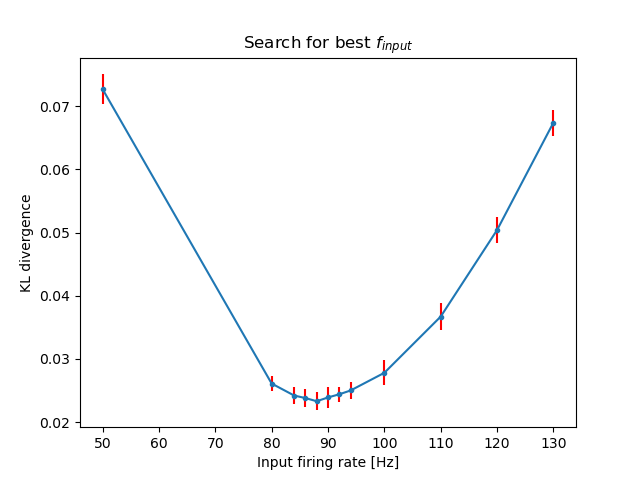
\includegraphics[width=\linewidth]{figures/1D/KLDvsfInput_fPrior0tau4.png}
  \caption{\textbf{KL divergence for different $f_{input}$ values.} Hyperparameters: $f_{prior} = 0 Hz, \tau_{decay} = 4 ms$}
  \label{fig:1D_KLD_fPrior0_tau4}
\end{figure}

\begin{figure}
  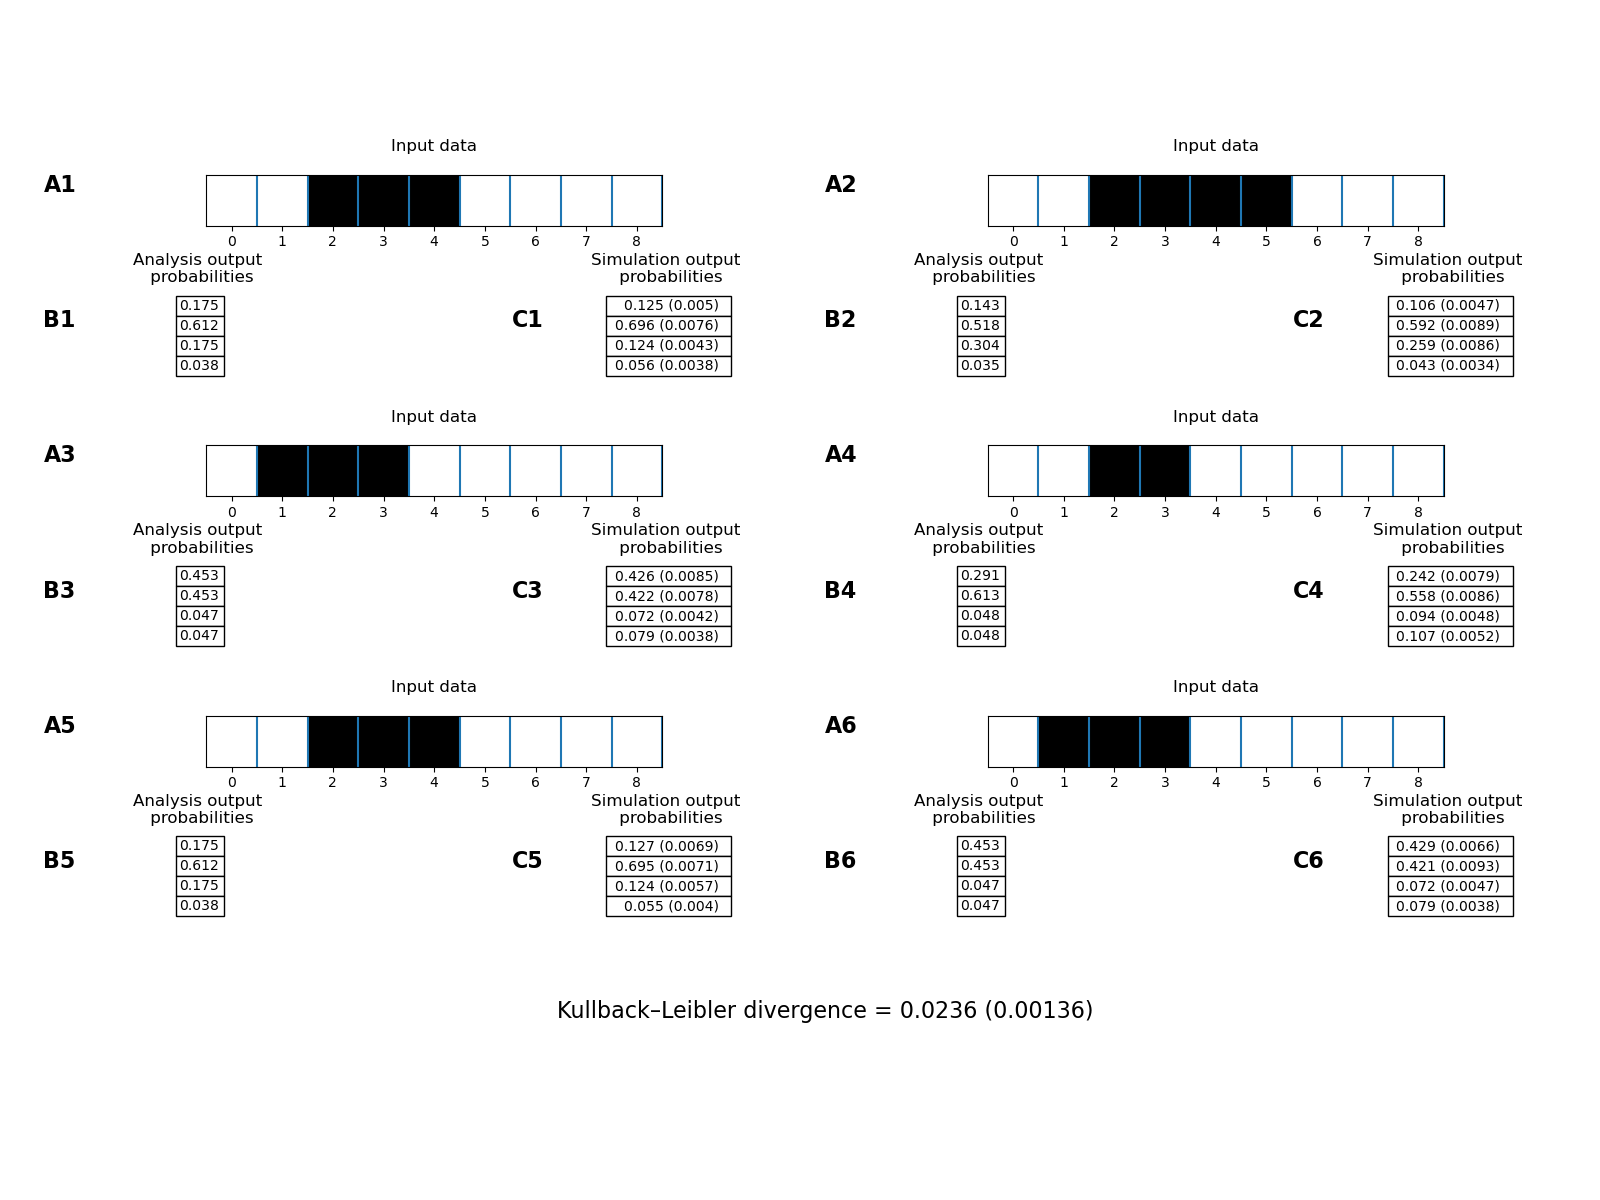
\includegraphics[width=\linewidth]{figures/1D/1D_88_0_4.png}
   \caption{\textbf{Analysis and simulation result. } Hyperparameters: $f_{input} = 88 Hz, f_{prior} = 0 Hz, \tau_{decay} = 4 ms$ \textbf{A} Input images with 9 x 1 pixels. \textbf{B} Analytically calculated posterior probabilities and simulated posterior probabilities. The standard deviations are given by the black bars.}
  \label{fig:1D_88_0_4}
\end{figure}

\begin{table}[]
\label{tab:1D_88_0_4}
\small
\tabcolsep=0.11cm
\begin{tabular}{|c|cc|cc|}
\hline
                       & \multicolumn{2}{c|}{Image 1}                       & \multicolumn{2}{c|}{Image 2}                       \\ \hline
                       & \multicolumn{1}{c|}{Analysis} & Simulation         & \multicolumn{1}{c|}{Analysis} & Simulation         \\ \hline
$y_0$                  & \multicolumn{1}{c|}{0.175}    & 0.126 $\pm$ 0.0050 & \multicolumn{1}{c|}{0.143}    & 0.106 $\pm$ 0.0054 \\ \hline
$y_1$                  & \multicolumn{1}{c|}{0.612}    & 0.695 $\pm$ 0.0066 & \multicolumn{1}{c|}{0.518}    & 0.587 $\pm$ 0.0098 \\ \hline
$y_2$                  & \multicolumn{1}{c|}{0.175}    & 0.124 $\pm$ 0.0049 & \multicolumn{1}{c|}{0.304}    & 0.264 $\pm$ 0.0072 \\ \hline
$y_3$                  & \multicolumn{1}{c|}{0.038}    & 0.054 $\pm$ 0.0039 & \multicolumn{1}{c|}{0.035}    & 0.043 $\pm$ 0.0028 \\ \hline
                       & \multicolumn{2}{c|}{Image 3}                       & \multicolumn{2}{c|}{Image 4}                       \\ \hline
$y_0$                  & \multicolumn{1}{c|}{0.453}    & 0.429 $\pm$ 0.0080 & \multicolumn{1}{c|}{0.291}    & 0.240 $\pm$ 0.0044 \\ \hline
$y_1$                  & \multicolumn{1}{c|}{0.453}    & 0.421 $\pm$ 0.0083 & \multicolumn{1}{c|}{0.613}    & 0.556 $\pm$ 0.0084 \\ \hline
$y_2$                  & \multicolumn{1}{c|}{0.047}    & 0.070 $\pm$ 0.0037 & \multicolumn{1}{c|}{0.048}    & 0.095 $\pm$ 0.0036 \\ \hline
$y_3$                  & \multicolumn{1}{c|}{0.047}    & 0.080 $\pm$ 0.0044 & \multicolumn{1}{c|}{0.048}    & 0.109 $\pm$ 0.0058 \\ \hline
						& \multicolumn{2}{c|}{Image 5}                       & \multicolumn{2}{c|}{Image 6}                       \\ \hline
$y_0$                  & \multicolumn{1}{c|}{0.175}    & 0.125 $\pm$ 0.0044 & \multicolumn{1}{c|}{0.453}    & 0.426 $\pm$ 0.0085 \\ \hline
$y_1$                  & \multicolumn{1}{c|}{0.612}    & 0.697 $\pm$ 0.0072 & \multicolumn{1}{c|}{0.453}    & 0.424 $\pm$ 0.0068 \\ \hline
$y_2$                  & \multicolumn{1}{c|}{0.175}    & 0.124 $\pm$ 0.0038 & \multicolumn{1}{c|}{0.047}    & 0.072 $\pm$ 0.0031 \\ \hline
$y_3$                  & \multicolumn{1}{c|}{0.038}    & 0.054 $\pm$ 0.0032 & \multicolumn{1}{c|}{0.047}    & 0.078 $\pm$ 0.0047 \\ \hline
\end{tabular}
\caption{\textbf{Analysis and simulation output probabilities. } Hyperparameters: $f_{input} = 88 Hz, f_{prior} = 0 Hz, \tau_{decay} = 4 ms$}
\end{table}

\paragraph{Simulation results with prior enabled}
After determining the best input firing rates for two different values of $\tau_{decay}$, the prior neurons were activated and the best $f_{prior}$ was searched.
\subparagraph{$\tau_{decay} = 0.015 seconds$, $f_{input} = 42 Hz$}
The search for the best value of $f_{prior}$ was performed in the same manner as for $f_{input}$. Values between 140 and 240 Hz were simulated and a prior firing rate of 222 Hz performed the best. The result of this search can be seen in Figure \ref{fig:1D_KLD_fInput42_tau15}. The simulation results can be seen in Figure \ref{fig:1D_42_222_15} and Table \ref{tab:1D_42_222_15}. In Figure \ref{fig:1D_42_222_15} the value of the prior is indicated by the red border which is three pixels wide and centered at the center position of the corresponding output class.

\begin{figure}
  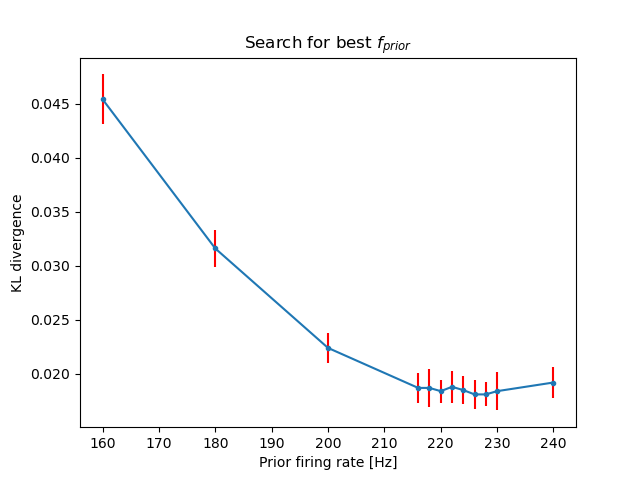
\includegraphics[width=\linewidth]{figures/1D/KLDvsfPrior_fInput42tau15.png}
  \caption{\textbf{KL divergence for different $f_{prior}$ values.} Hyperparameters: $f_{input} = 42 Hz, \tau_{decay} = 15 ms$}
  \label{fig:1D_KLD_fInput42_tau15}
\end{figure}

\begin{figure}
  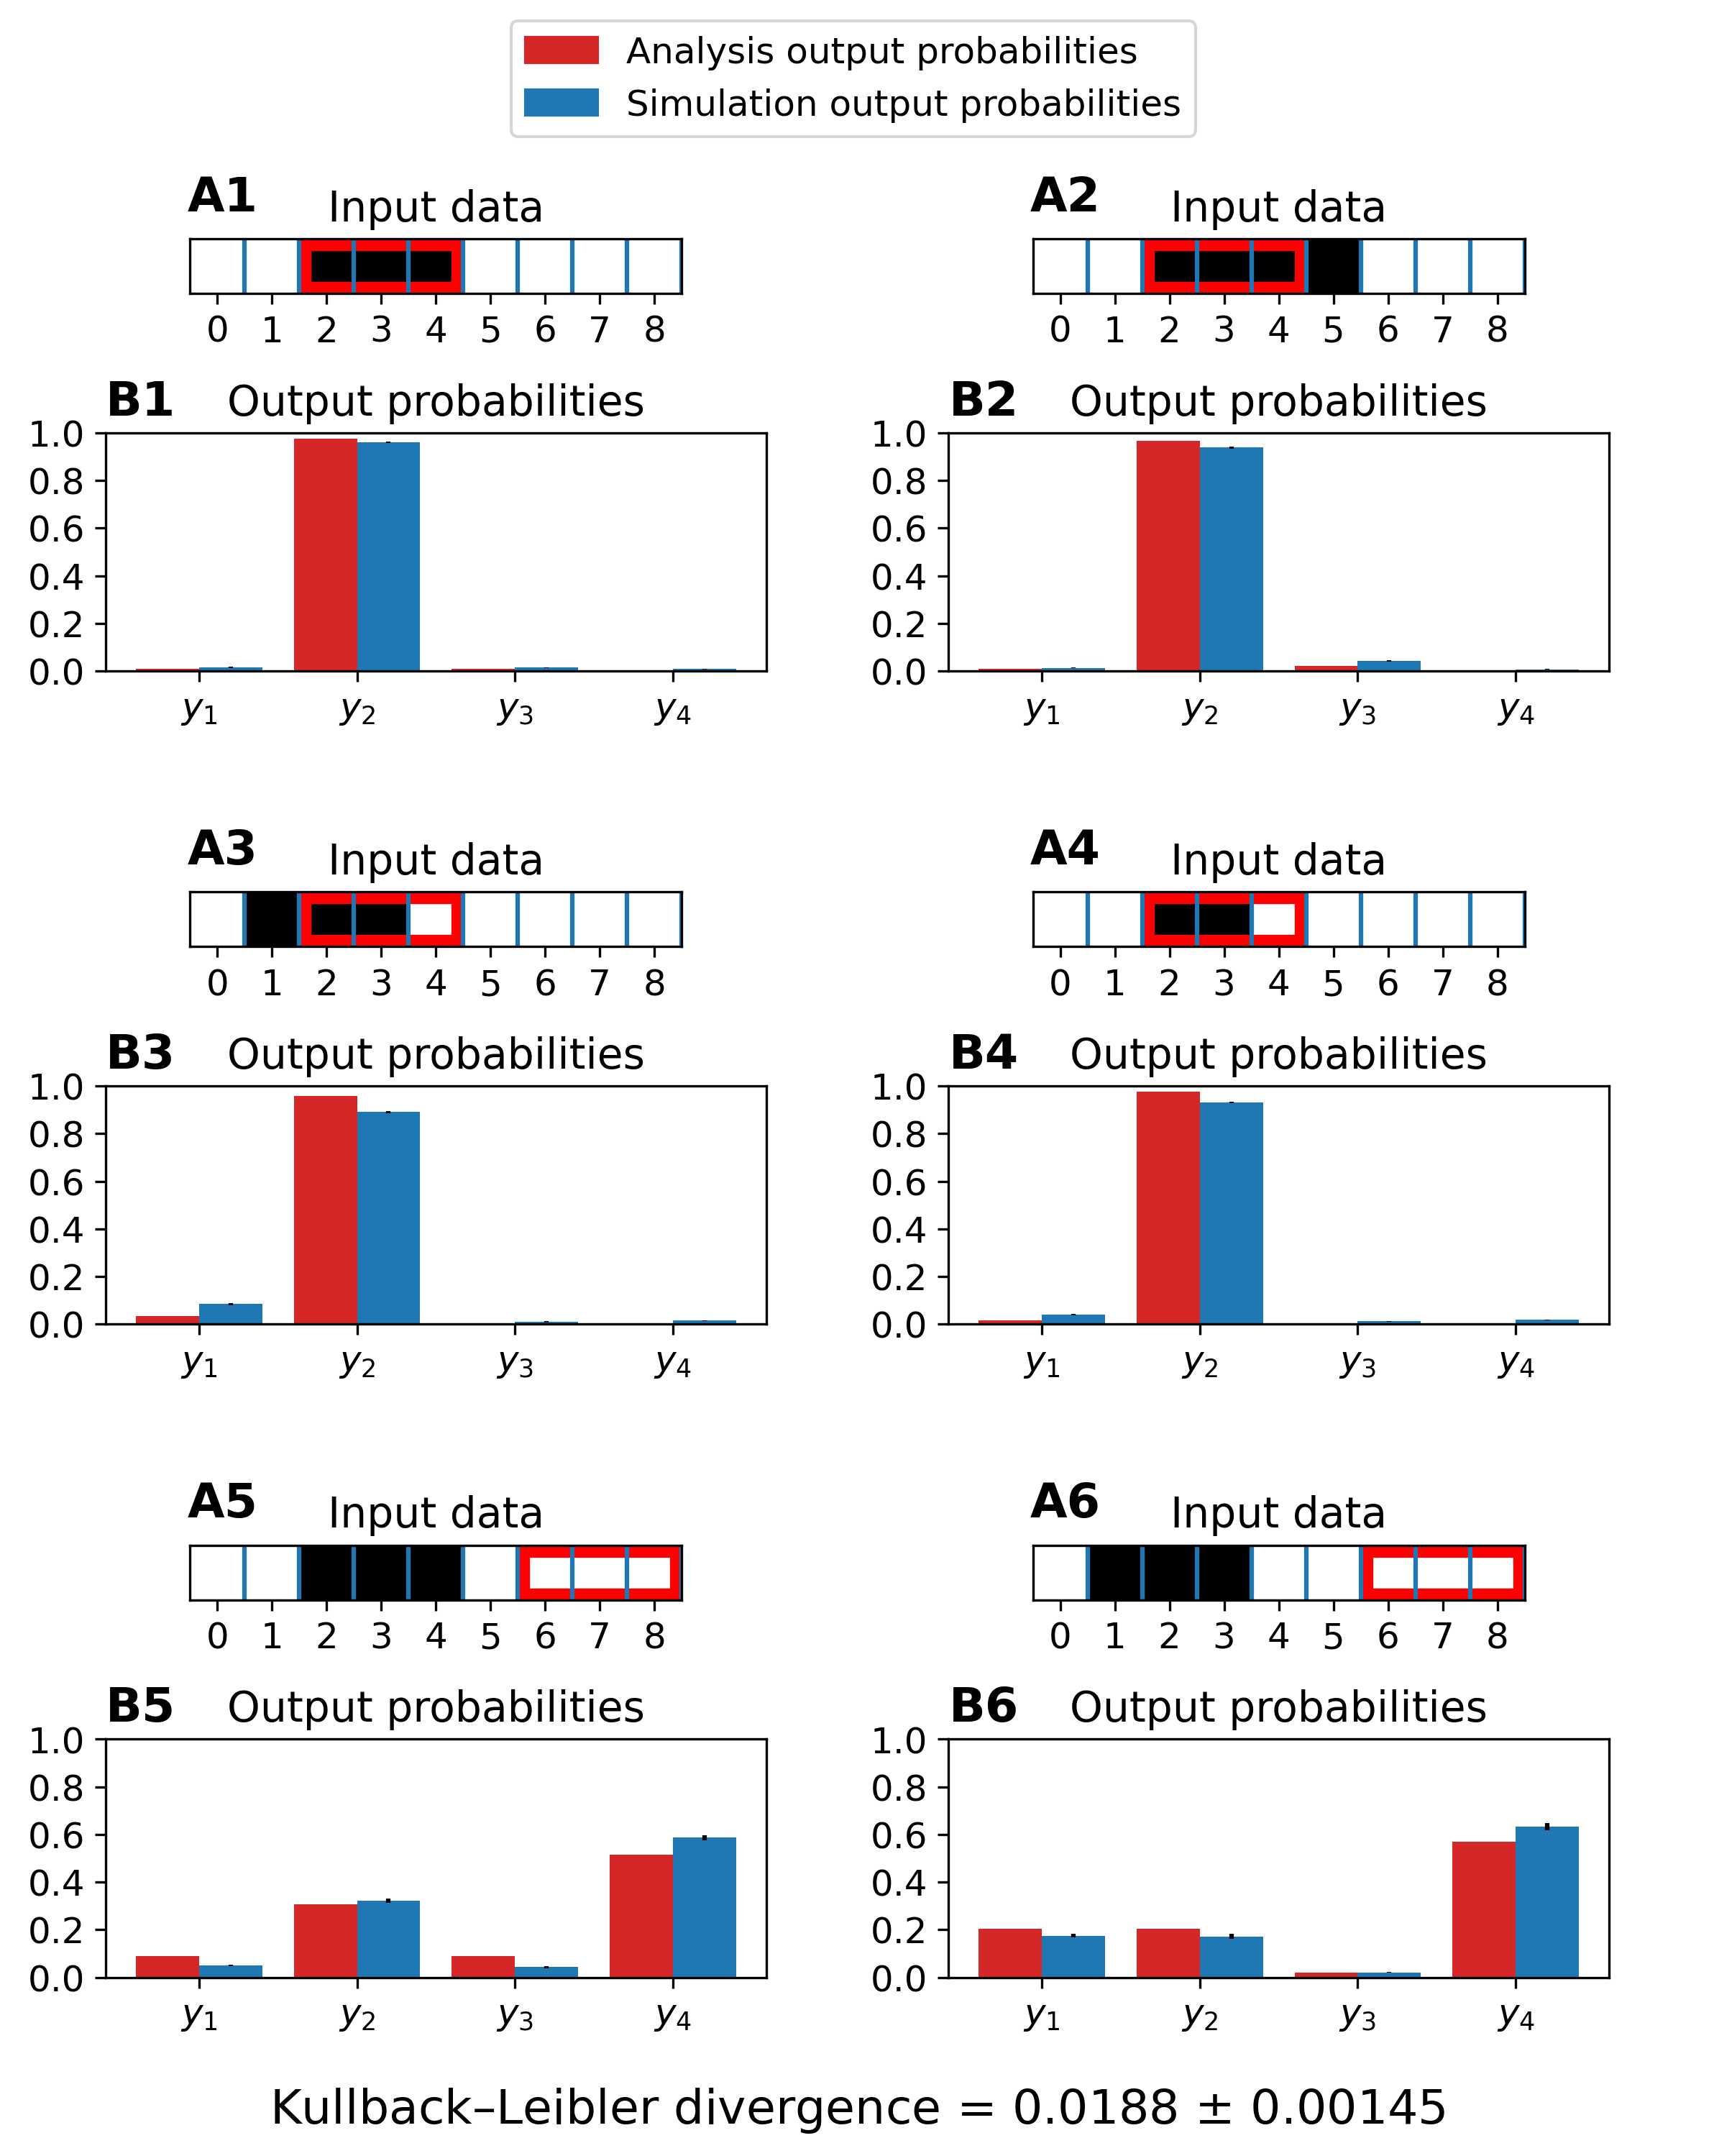
\includegraphics[width=\linewidth]{figures/1D/1D_42_222_15.png}
     \caption{\textbf{Analysis and simulation result. } Hyperparameters: $f_{input} = 42 Hz, f_{prior} = 222 Hz, \tau_{decay} = 15 ms$ \textbf{A} Input images with 9 x 1 pixels. Prior given as red border. \textbf{B} Analytically calculated posterior probabilities and simulated posterior probabilities. The standard deviations are given by the black bars.}
  \label{fig:1D_42_222_15}
\end{figure}

\begin{table}[]
\label{tab:1D_42_222_15}
\small
\tabcolsep=0.11cm
\begin{tabular}{|c|cc|cc|}
\hline
                       & \multicolumn{2}{c|}{Image 1}                       & \multicolumn{2}{c|}{Image 2}                       \\ \hline
                       & \multicolumn{1}{c|}{Analysis} & Simulation         & \multicolumn{1}{c|}{Analysis} & Simulation         \\ \hline
$y_0$                  & \multicolumn{1}{c|}{0.010}    & 0.015 $\pm$ 0.0021 & \multicolumn{1}{c|}{0.010}    & 0.013 $\pm$ 0.0016 \\ \hline
$y_1$                  & \multicolumn{1}{c|}{0.977}    & 0.962 $\pm$ 0.0030 & \multicolumn{1}{c|}{0.967}    & 0.938 $\pm$ 0.0040 \\ \hline
$y_2$                  & \multicolumn{1}{c|}{0.010}    & 0.015 $\pm$ 0.0017 & \multicolumn{1}{c|}{0.021}    & 0.042 $\pm$ 0.0032 \\ \hline
$y_3$                  & \multicolumn{1}{c|}{0.002}    & 0.008 $\pm$ 0.0016 & \multicolumn{1}{c|}{0.002}    & 0.007 $\pm$ 0.0013 \\ \hline
                       & \multicolumn{2}{c|}{Image 3}                       & \multicolumn{2}{c|}{Image 4}                       \\ \hline
$y_0$                  & \multicolumn{1}{c|}{0.035}    & 0.084 $\pm$ 0.0038 & \multicolumn{1}{c|}{0.017}    & 0.039 $\pm$ 0.0033 \\ \hline
$y_1$                  & \multicolumn{1}{c|}{0.957}    & 0.891 $\pm$ 0.0046 & \multicolumn{1}{c|}{0.977}    & 0.931 $\pm$ 0.0045 \\ \hline
$y_2$                  & \multicolumn{1}{c|}{0.004}    & 0.010 $\pm$ 0.0018 & \multicolumn{1}{c|}{0.003}    & 0.012 $\pm$ 0.0017 \\ \hline
$y_3$                  & \multicolumn{1}{c|}{0.004}    & 0.015 $\pm$ 0.0016 & \multicolumn{1}{c|}{0.003}    & 0.018 $\pm$ 0.0024 \\ \hline
						& \multicolumn{2}{c|}{Image 5}                       & \multicolumn{2}{c|}{Image 6}                       \\ \hline
$y_0$                  & \multicolumn{1}{c|}{0.088}    & 0.050 $\pm$ 0.0033 & \multicolumn{1}{c|}{0.205}    & 0.175 $\pm$ 0.0077 \\ \hline
$y_1$                  & \multicolumn{1}{c|}{0.308}    & 0.321 $\pm$ 0.0087 & \multicolumn{1}{c|}{0.205}    & 0.172 $\pm$ 0.0106 \\ \hline
$y_2$                  & \multicolumn{1}{c|}{0.088}    & 0.043 $\pm$ 0.0039 & \multicolumn{1}{c|}{0.021}    & 0.021 $\pm$ 0.0018 \\ \hline
$y_3$                  & \multicolumn{1}{c|}{0.515}    & 0.587 $\pm$ 0.0105 & \multicolumn{1}{c|}{0.570}    & 0.632 $\pm$ 0.0158 \\ \hline
\end{tabular}
\caption{\textbf{Analysis and simulation output probabilities. } Hyperparameters: $f_{input} = 42 Hz, f_{prior} = 222 Hz, \tau_{decay} = 15 ms$}
\end{table}

\subparagraph{$\tau_{decay} = 0.004 seconds$, $f_{input} = 88 Hz$}
The search for the best value of $f_{prior}$ was performed in the same manner as for $f_{input}$. Values between 360 and 460 Hz were simulated and a prior firing rate of 440 Hz performed the best. The result of this search can be seen in Figure \ref{fig:1D_KLD_fInput88_tau4}. The results of this hyperparameter combination are given in Figure \ref{fig:1D_88_440_4} and Table \ref{tab:1D_88_440_4}.

\begin{figure}
  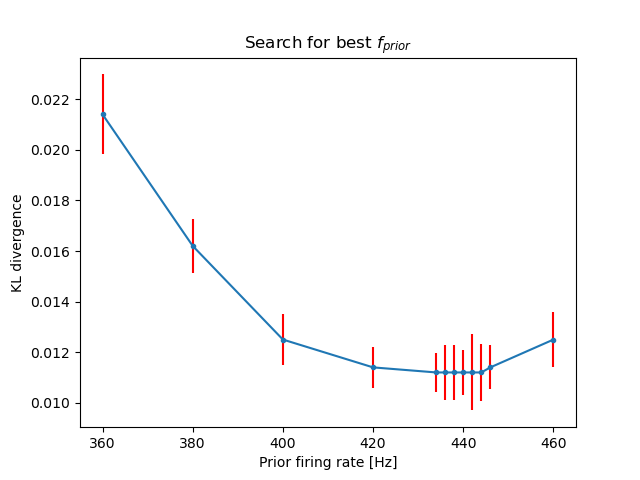
\includegraphics[width=\linewidth]{figures/1D/KLDvsfPrior_fInput88tau4.png}
  \caption{\textbf{KL divergence for different $f_{prior}$ values.} Hyperparameters: $f_{input} = 88 Hz, \tau_{decay} = 4 ms$}
  \label{fig:1D_KLD_fInput88_tau4}
\end{figure}

\begin{figure}
  \includegraphics[width=\linewidth]{figures/1D/1D_88_440_4.png}
       \caption{\textbf{Analysis and simulation result. } Hyperparameters: $f_{input} = 88 Hz, f_{prior} = 440 Hz, \tau_{decay} = 4 ms$ \textbf{A} Input images with 9 x 1 pixels. Prior given as red border. \textbf{B} Analytically calculated posterior probabilities and simulated posterior probabilities. The standard deviations are given by the black bars.}
  \label{fig:1D_88_440_4}
\end{figure}

\begin{table}[]
\label{tab:1D_88_440_4}
\small
\tabcolsep=0.11cm
\begin{tabular}{|c|cc|cc|}
\hline
                       & \multicolumn{2}{c|}{Image 1}                       & \multicolumn{2}{c|}{Image 2}                       \\ \hline
                       & \multicolumn{1}{c|}{Analysis} & Simulation         & \multicolumn{1}{c|}{Analysis} & Simulation         \\ \hline
$y_0$                  & \multicolumn{1}{c|}{0.010}    & 0.011 $\pm$ 0.0016 & \multicolumn{1}{c|}{0.010}    & 0.010 $\pm$ 0.0017 \\ \hline
$y_1$                  & \multicolumn{1}{c|}{0.977}    & 0.974 $\pm$ 0.0026 & \multicolumn{1}{c|}{0.967}    & 0.957 $\pm$ 0.0034 \\ \hline
$y_2$                  & \multicolumn{1}{c|}{0.010}    & 0.010 $\pm$ 0.0019 & \multicolumn{1}{c|}{0.021}    & 0.028 $\pm$ 0.0036 \\ \hline
$y_3$                  & \multicolumn{1}{c|}{0.002}    & 0.005 $\pm$ 0.0013 & \multicolumn{1}{c|}{0.002}    & 0.005 $\pm$ 0.0011 \\ \hline
                       & \multicolumn{2}{c|}{Image 3}                       & \multicolumn{2}{c|}{Image 4}                       \\ \hline
$y_0$                  & \multicolumn{1}{c|}{0.035}    & 0.066 $\pm$ 0.0031 & \multicolumn{1}{c|}{0.017}    & 0.026 $\pm$ 0.0030 \\ \hline
$y_1$                  & \multicolumn{1}{c|}{0.957}    & 0.915 $\pm$ 0.0044 & \multicolumn{1}{c|}{0.977}    & 0.952 $\pm$ 0.0039 \\ \hline
$y_2$                  & \multicolumn{1}{c|}{0.004}    & 0.009 $\pm$ 0.0014 & \multicolumn{1}{c|}{0.003}    & 0.009 $\pm$ 0.0017 \\ \hline
$y_3$                  & \multicolumn{1}{c|}{0.004}    & 0.011 $\pm$ 0.0018 & \multicolumn{1}{c|}{0.003}    & 0.012 $\pm$ 0.0020 \\ \hline
						& \multicolumn{2}{c|}{Image 5}                       & \multicolumn{2}{c|}{Image 6}                       \\ \hline
$y_0$                  & \multicolumn{1}{c|}{0.088}    & 0.052 $\pm$ 0.0027 & \multicolumn{1}{c|}{0.205}    & 0.172 $\pm$ 0.0061 \\ \hline
$y_1$                  & \multicolumn{1}{c|}{0.308}    & 0.328 $\pm$ 0.0085 & \multicolumn{1}{c|}{0.205}    & 0.174 $\pm$ 0.0059 \\ \hline
$y_2$                  & \multicolumn{1}{c|}{0.088}    & 0.046 $\pm$ 0.0031 & \multicolumn{1}{c|}{0.021}    & 0.025 $\pm$ 0.0025 \\ \hline
$y_3$                  & \multicolumn{1}{c|}{0.515}    & 0.573 $\pm$ 0.0089 & \multicolumn{1}{c|}{0.570}    & 0.630 $\pm$ 0.0095 \\ \hline
\end{tabular}
\caption{\textbf{Analysis and simulation output probabilities. } Hyperparameters: $f_{input} = 88 Hz, f_{prior} = 440 Hz, \tau_{decay} = 4 ms$}
\end{table}


To demonstrate the impact of rising $f_{prior}$ it was set to 600 Hz and the results can be seen in Figure \ref{fig:1D_88_600_4} and Table \ref{tab:1D_88_600_4}.

\begin{figure}
  \includegraphics[width=\linewidth]{figures/1D/1D_88_600_4.png}
  \caption{\textbf{Analysis and simulation result. } Hyperparameters: $f_{input} = 88 Hz, f_{prior} = 600 Hz, \tau_{decay} = 4 ms$ \textbf{A} Input images with 9 x 1 pixels. Prior given as red border. \textbf{B} Analytically calculated posterior probabilities and simulated posterior probabilities. The standard deviations are given by the black bars.}
  \label{fig:1D_88_600_4}
\end{figure}

\begin{table}[]
\label{tab:1D_88_600_4}
\small
\tabcolsep=0.11cm
\begin{tabular}{|c|cc|cc|}
\hline
                       & \multicolumn{2}{c|}{Image 1}                       & \multicolumn{2}{c|}{Image 2}                       \\ \hline
                       & \multicolumn{1}{c|}{Analysis} & Simulation         & \multicolumn{1}{c|}{Analysis} & Simulation         \\ \hline
$y_0$                  & \multicolumn{1}{c|}{0.010}    & 0.003 $\pm$ 0.0011 & \multicolumn{1}{c|}{0.010}    & 0.003 $\pm$ 0.0009 \\ \hline
$y_1$                  & \multicolumn{1}{c|}{0.977}    & 0.993 $\pm$ 0.0013 & \multicolumn{1}{c|}{0.967}    & 0.987 $\pm$ 0.0024 \\ \hline
$y_2$                  & \multicolumn{1}{c|}{0.010}    & 0.003 $\pm$ 0.0008 & \multicolumn{1}{c|}{0.021}    & 0.009 $\pm$ 0.0019 \\ \hline
$y_3$                  & \multicolumn{1}{c|}{0.002}    & 0.001 $\pm$ 0.0005 & \multicolumn{1}{c|}{0.002}    & 0.001 $\pm$ 0.0008 \\ \hline
                       & \multicolumn{2}{c|}{Image 3}                       & \multicolumn{2}{c|}{Image 4}                       \\ \hline
$y_0$                  & \multicolumn{1}{c|}{0.035}    & 0.023 $\pm$ 0.0025 & \multicolumn{1}{c|}{0.017}    & 0.008 $\pm$ 0.0011 \\ \hline
$y_1$                  & \multicolumn{1}{c|}{0.957}    & 0.971 $\pm$ 0.0030 & \multicolumn{1}{c|}{0.977}    & 0.984 $\pm$ 0.0019 \\ \hline
$y_2$                  & \multicolumn{1}{c|}{0.004}    & 0.003 $\pm$ 0.0009 & \multicolumn{1}{c|}{0.003}    & 0.003 $\pm$ 0.0008 \\ \hline
$y_3$                  & \multicolumn{1}{c|}{0.004}    & 0.003 $\pm$ 0.0011 & \multicolumn{1}{c|}{0.003}    & 0.004 $\pm$ 0.0011 \\ \hline
						& \multicolumn{2}{c|}{Image 5}                       & \multicolumn{2}{c|}{Image 6}                       \\ \hline
$y_0$                  & \multicolumn{1}{c|}{0.088}    & 0.028 $\pm$ 0.0026 & \multicolumn{1}{c|}{0.205}    & 0.089 $\pm$ 0.0057 \\ \hline
$y_1$                  & \multicolumn{1}{c|}{0.308}    & 0.182 $\pm$ 0.0077 & \multicolumn{1}{c|}{0.205}    & 0.088 $\pm$ 0.0047 \\ \hline
$y_2$                  & \multicolumn{1}{c|}{0.088}    & 0.023 $\pm$ 0.0025 & \multicolumn{1}{c|}{0.021}    & 0.010 $\pm$ 0.0016 \\ \hline
$y_3$                  & \multicolumn{1}{c|}{0.515}    & 0.766 $\pm$ 0.0079 & \multicolumn{1}{c|}{0.570}    & 0.813 $\pm$ 0.0081 \\ \hline
\end{tabular}
\caption{\textbf{Analysis and simulation output probabilities. } Hyperparameters: $f_{input} = 88 Hz, f_{prior} = 600 Hz, \tau_{decay} = 4 ms$}
\end{table}

\subparagraph{$\tau_{decay} = 0.004 seconds$, $f_{input} = 98$, $f_{prior} = 440 Hz$}
Finally it was tested if a increase of $f_{input}$ might decrease the Kullback-Leibler divergence even further. The network was simulated with increasing values of $f_{input}$ in steps of 2 Hz, beginning from 90 Hz. The result of this search can be seen in Figure \ref{fig:1D_KLD_fPrior440_tau4}. The best result was obtained with an input firing rate of 98 Hz. The results of that simulation can be seen in Figure \ref{fig:1D_98_440_4} and Table \ref{tab:1D_98_440_4}.

\begin{figure}
  \includegraphics[width=\linewidth]{figures/1D/KLDvsfInput_fPrior440tau4.png}
  \caption{\textbf{KL divergence for different $f_{input}$ values.} Hyperparameters: $f_{prior} = 440 Hz, \tau_{decay} = 4 ms$}
  \label{fig:1D_KLD_fPrior440_tau4}
\end{figure}

\begin{figure}
  \includegraphics[width=\linewidth]{figures/1D/1D_98_440_4.png}
    \caption{\textbf{Analysis and simulation result. } Hyperparameters: $f_{input} = 98 Hz, f_{prior} = 440 Hz, \tau_{decay} = 4 ms$ \textbf{A} Input images with 9 x 1 pixels. Prior given as red border. \textbf{B} Analytically calculated posterior probabilities and simulated posterior probabilities. The standard deviations are given by the black bars.}
  \label{fig:1D_98_440_4}
\end{figure}

\begin{table}[]
\label{tab:1D_98_440_4}
\small
\tabcolsep=0.11cm
\begin{tabular}{|c|cc|cc|}
\hline
                       & \multicolumn{2}{c|}{Image 1}                       & \multicolumn{2}{c|}{Image 2}                       \\ \hline
                       & \multicolumn{1}{c|}{Analysis} & Simulation         & \multicolumn{1}{c|}{Analysis} & Simulation         \\ \hline
$y_0$                  & \multicolumn{1}{c|}{0.010}    & 0.009 $\pm$ 0.0016 & \multicolumn{1}{c|}{0.010}    & 0.009 $\pm$ 0.0015 \\ \hline
$y_1$                  & \multicolumn{1}{c|}{0.977}    & 0.979 $\pm$ 0.0020 & \multicolumn{1}{c|}{0.967}    & 0.963 $\pm$ 0.0023 \\ \hline
$y_2$                  & \multicolumn{1}{c|}{0.010}    & 0.009 $\pm$ 0.0010 & \multicolumn{1}{c|}{0.021}    & 0.025 $\pm$ 0.0020 \\ \hline
$y_3$                  & \multicolumn{1}{c|}{0.002}    & 0.004 $\pm$ 0.0009 & \multicolumn{1}{c|}{0.002}    & 0.003 $\pm$ 0.0008 \\ \hline
                       & \multicolumn{2}{c|}{Image 3}                       & \multicolumn{2}{c|}{Image 4}                       \\ \hline
$y_0$                  & \multicolumn{1}{c|}{0.035}    & 0.067 $\pm$ 0.0051 & \multicolumn{1}{c|}{0.017}    & 0.025 $\pm$ 0.0031 \\ \hline
$y_1$                  & \multicolumn{1}{c|}{0.957}    & 0.916 $\pm$ 0.0051 & \multicolumn{1}{c|}{0.977}    & 0.955 $\pm$ 0.0033 \\ \hline
$y_2$                  & \multicolumn{1}{c|}{0.004}    & 0.007 $\pm$ 0.0012 & \multicolumn{1}{c|}{0.003}    & 0.009 $\pm$ 0.0012 \\ \hline
$y_3$                  & \multicolumn{1}{c|}{0.004}    & 0.009 $\pm$ 0.0019 & \multicolumn{1}{c|}{0.003}    & 0.011 $\pm$ 0.0019 \\ \hline
						& \multicolumn{2}{c|}{Image 5}                       & \multicolumn{2}{c|}{Image 6}                       \\ \hline
$y_0$                  & \multicolumn{1}{c|}{0.088}    & 0.051 $\pm$ 0.0035 & \multicolumn{1}{c|}{0.205}    & 0.191 $\pm$ 0.0080 \\ \hline
$y_1$                  & \multicolumn{1}{c|}{0.308}    & 0.379 $\pm$ 0.0084 & \multicolumn{1}{c|}{0.205}    & 0.188 $\pm$ 0.0061 \\ \hline
$y_2$                  & \multicolumn{1}{c|}{0.088}    & 0.046 $\pm$ 0.0027 & \multicolumn{1}{c|}{0.021}    & 0.022 $\pm$ 0.0021 \\ \hline
$y_3$                  & \multicolumn{1}{c|}{0.515}    & 0.523 $\pm$ 0.0084 & \multicolumn{1}{c|}{0.570}    & 0.600 $\pm$ 0.0116 \\ \hline
\end{tabular}
\caption{\textbf{Analysis and simulation output probabilities. } Hyperparameters: $f_{input} = 98 Hz, f_{prior} = 440 Hz, \tau_{decay} = 4 ms$}
\end{table}

\paragraph{Approximating the analytic solution}
After first finding the optimal $f_{input}$ for disabled prior activity and then finding the optimal $f_{prior}$ with enabled prior activity for $\tau_{decay}$ the simulation was not yet approximating the analytical solution perfectly. Because of that it was tried to raise $f_{input}$ to further decrease the Kullback-Leibler divergence. The further search for a better $f_{input}$ was performed for $\tau_{decay} = 0.004 ms$ and $f_{prior} = 440 Hz$, as this set of hyperparameters performed the best overall.
When comparing the former optimal result in Figure \ref{fig:1D_88_440_4} with $f_{input} = 88 Hz$, to the result with $f_{input} = 98 Hz$ in Figure \ref{fig:1D_98_440_4}, it can be seen that the Kullback-Leibler divergence decreased from 0.0112 to 0.0101. However, when comparing Tables \ref{tab:1D_88_440_4} and \ref{tab:1D_98_440_4}, it can be seen that the higher $f_{input}$ did not perform strictly better. The simulation output probabilities for Image 3 improved, while for Image 5 the output probability of $y_2$ diverged more. A further increase of $f_{input}$ started to increase the Kullback-Leibler divergence again, thus the final optimum of the hyperparameter set was reached. It was assumed that increasing $f_{input}$ after $f_{prior}$ was fitted was necessary because the overall impact of $f_{input}$ on the simulation decreased due to the introduction of the prior activity.

\subsection{Impact of the hyperparameters}
\label{subsection:impactHyper}
\paragraph{$f_{input}$} controls how strongly the information of the pixels of the input image is weighed. This means that by raising $f_{input}$ the impact of the active pixels increases, while the impact of the prior neuron decreases comparatively. This effect will be shown in the following paragraph about $f_{prior}$. Furthermore, by raising $f_{input}$ the membrane potentials of all output neurons are raised equally by the same percentage. However, this causes difficulties when trying to determine the optimal $f_{input}$. When raising $f_{input}$ it was also observed that the posteriors of output classes adjacent to the active pixels decreased. This can be observed when comparing Tables \ref{tab:1D_42_0_15} and \ref{tab:1D_70_0_15} where $f_{input}$ was raised from 42 Hz to 70 Hz. For example when looking at Image 4 in the mentioned tables, it can be seen that for $f_{input} = 42 Hz$ the simulation output probability of $y_1$ is 0.245. This probability is due to the active pixel at position 2, which belongs to class 1 and 2 at the same time. $y_2$ has a higher simulation output probability of 0.553, as it has two active pixels within its active area. When increasing $f_{input}$ to 70 Hz one might expect the probabilities for $y_1$ and $y_2$ to rise. This however does not happen, instead the simulation output probability for $y_1$ fell to 0.207, while for $y_2$ it rose to 0.685. It is assumed that this happened because the membrane potentials of the output neurons were never normalized. As the input neurons spike more quickly the membrane potential of $y_1$ rose by a smaller amount than the membrane potential of $y_2$, as there was one more active pixel within the active area of $y_2$. As given by Equation \ref{eqn:qk} $q$ depends exponentially on $u_k$. This means that its probability density function changes if all membrane potentials are changed by the same percentage, which is exactly what happens when $f_{input}$ is increased. However, this behaviour might be desired, as generating more input spikes corresponds stochastically to taking more samples from the likelihood probability distribution. Pulling more samples reduces the standard error of the posterior probability distribution, thus reducing the width of its probability density function. This means that the more samples of the input the network takes, the more certain it becomes of the most likely option, which is output class 2.

\paragraph{$f_{prior}$} When increasing the prior firing rate the impact on the result of the prior neurons increased, while the impact of the input neurons decreased comparatively. When comparing the Figures \ref{fig:1D_88_440_4} and \ref{fig:1D_88_600_4} which show the results for $f_{input} = 88 Hz$, $\tau_{decay} = 4 ms$ and $f_{prior} = 440$ and $600 Hz$ respectively it can be seen under B6 how the simulation output probability for $y_4$ rose, while all other probabilities fell. The opposite behaviour can be observed when raising $f_{input}$ instead.

\paragraph{$\tau_{decay}$} determines for how long and how strongly an input or prior spike contributes to the membrane potentials of the output neurons. The bigger $\tau_{decay}$ is, the smaller $f_{input}$ and $f_{prior}$ need to be, to minimize the Kullback-Leibler divergence. This is represented by the final hyperparameters for $\tau_{decay}$ of 4 and 15 ms. While for $\tau_{decay} = 15 ms$ the best input firing rate was 42 Hz and the prior firing rate was 222 Hz, for $\tau_{decay} = 4 ms$ they had to be raised to 98 and 440 Hz to minimize the Kullback-Leibler divergence.

\section{Experiment 3: Transferability of hyperparameters}
\label{section:1DDoubleSize}

\subsection{Introduction}
In this experiment the optimal hyperparameters determined in Experiment 2 were used, while doubling the size of the network and input images of Experiment 2. The goal was to determine if the hyperparameters are universally applicable, regardless of the network size.

\subsection{Methods}
The number input neurons was doubled from 18 to 36 neurons. This resulted in input images with 18 pixels. To double the effect of the prior neurons $f_{prior}$ was doubled to 880 Hz, while the amount of the prior neurons was kept the same with 4 prior neurons. Furthermore the matrix $P^{X|Y}$ was doubled in size by copying each value of the matrix to the right of itself.  The rest of the methods were performed analogously to Experiment 2.

\subsection{Results}

The expanded matrix $P^{X|Y}$ had its columns doubled, resulting in a dimension of $[18 \times 4]$. This yielded

\setcounter{MaxMatrixCols}{18}

\begin{equation}
\footnotesize
\label{eqn:pXvorausgesetztYResultDoubled}
\begin{matrix}
P^{X|Y} = \\
\begin{bmatrix}
0.9 & 0.9 & 0.9 & 0.9 & 0.9 & 0.9 & 0.1 & 0.1 & 0.1 & 0.1 & 0.1 & 0.1 & 0.1 & 0.1 & 0.1 & 0.1 & 0.1 & 0.1\\
0.1 & 0.1 & 0.1 & 0.1 & 0.9 & 0.9 & 0.9 & 0.9 & 0.9 & 0.9 & 0.1 & 0.1 & 0.1 & 0.1 & 0.1 & 0.1 & 0.1 & 0.1\\
0.1 & 0.1 & 0.1 & 0.1 & 0.1 & 0.1 & 0.1 & 0.1 & 0.9 & 0.9 & 0.9 & 0.9 & 0.9 & 0.9 & 0.1 & 0.1 & 0.1 & 0.1\\
0.1 & 0.1 & 0.1 & 0.1 & 0.1 & 0.1 & 0.1 & 0.1 & 0.1 & 0.1 & 0.1 & 0.1 & 0.9 & 0.9 & 0.9 & 0.9 & 0.9 & 0.9\\
\end{bmatrix}.
\end{matrix}
\end{equation}

The simulation result for $f_{input} = 98 Hz$, $f_{prior} = 880 Hz$ and $\tau_{decay} = 4 ms$ can be seen in Figure \ref{fig:doubleSize_98_880_4} and Table \ref{tab:doubleSize_98_880_4}. Initially the Kullback-Leibler divergence was infinite in this result, because some simulation output probabilities were zero and the Kullback-Leibler divergence is not defined for probabilities of zero. To circumvent this an approximated Kullback-Leibler divergence was calculated by setting the simulation output probabilities that were 0 to 0.0000001. This yielded a Kullback-Leibler divergence of 0.2392.
\begin{figure}
  \includegraphics[width=\linewidth]{figures/1D/doubleSize/doubleSize_98_880_4.png}
      \caption{\textbf{Analysis and simulation result. } Hyperparameters: $f_{input} = 98 Hz, f_{prior} = 880 Hz, \tau_{decay} = 4 ms$ \textbf{A} Input images with 18 x 1 pixels. Prior given as red border. \textbf{B} Analytically calculated posterior probabilities and simulated posterior probabilities. The standard deviations are given by the black bars.}
  \label{fig:doubleSize_98_880_4}
\end{figure}

\begin{table}[]
\label{tab:doubleSize_98_880_4}
\small
\tabcolsep=0.11cm
\begin{tabular}{|c|cc|cc|}
\hline
                       & \multicolumn{2}{c|}{Image 1}                       & \multicolumn{2}{c|}{Image 2}                       \\ \hline
                       & \multicolumn{1}{c|}{Analysis} & Simulation         & \multicolumn{1}{c|}{Analysis} & Simulation         \\ \hline
$y_0$                  & \multicolumn{1}{c|}{0.010}    & 0.000 $\pm$ 0.0001 & \multicolumn{1}{c|}{0.010}    & 0.000 $\pm$ 0.0001 \\ \hline
$y_1$                  & \multicolumn{1}{c|}{0.977}    & 1.000 $\pm$ 0.0002 & \multicolumn{1}{c|}{0.967}    & 1.000 $\pm$ 0.0003 \\ \hline
$y_2$                  & \multicolumn{1}{c|}{0.010}    & 0.000 $\pm$ 0.0001 & \multicolumn{1}{c|}{0.021}    & 0.000 $\pm$ 0.0002 \\ \hline
$y_3$                  & \multicolumn{1}{c|}{0.002}    & 0.000 $\pm$ 0.0000 & \multicolumn{1}{c|}{0.002}    & 0.000 $\pm$ 0.0001 \\ \hline
                       & \multicolumn{2}{c|}{Image 3}                       & \multicolumn{2}{c|}{Image 4}                       \\ \hline
$y_0$                  & \multicolumn{1}{c|}{0.035}    & 0.003 $\pm$ 0.0010 & \multicolumn{1}{c|}{0.017}    & 0.000 $\pm$ 0.0004 \\ \hline
$y_1$                  & \multicolumn{1}{c|}{0.957}    & 0.997 $\pm$ 0.0010 & \multicolumn{1}{c|}{0.977}    & 1.000 $\pm$ 0.0004 \\ \hline
$y_2$                  & \multicolumn{1}{c|}{0.004}    & 0.000 $\pm$ 0.0001 & \multicolumn{1}{c|}{0.003}    & 0.000 $\pm$ 0.0001 \\ \hline
$y_3$                  & \multicolumn{1}{c|}{0.004}    & 0.000 $\pm$ 0.0001 & \multicolumn{1}{c|}{0.003}    & 0.000 $\pm$ 0.0001 \\ \hline
						& \multicolumn{2}{c|}{Image 5}                       & \multicolumn{2}{c|}{Image 6}                       \\ \hline
$y_0$                  & \multicolumn{1}{c|}{0.088}    & 0.007 $\pm$ 0.0010 & \multicolumn{1}{c|}{0.205}    & 0.106 $\pm$ 0.0060 \\ \hline
$y_1$                  & \multicolumn{1}{c|}{0.308}    & 0.369 $\pm$ 0.0096 & \multicolumn{1}{c|}{0.205}    & 0.109 $\pm$ 0.0042 \\ \hline
$y_2$                  & \multicolumn{1}{c|}{0.088}    & 0.005 $\pm$ 0.0010 & \multicolumn{1}{c|}{0.021}    & 0.001 $\pm$ 0.0004 \\ \hline
$y_3$                  & \multicolumn{1}{c|}{0.515}    & 0.619 $\pm$ 0.0098 & \multicolumn{1}{c|}{0.570}    & 0.783 $\pm$ 0.0091 \\ \hline
\end{tabular}
\caption{\textbf{Analysis and simulation output probabilities. } Hyperparameters: $f_{input} = 98 Hz, f_{prior} = 880 Hz, \tau_{decay} = 4 ms$}
\end{table}

When comparing Figures \ref{fig:1D_98_440_4} and \ref{fig:doubleSize_98_880_4} it can be seen that the analysis output probabilities stayed the same. This was expected, as by doubling the pixels of the input images the information within them does not change. The areas corresponding to an output class doubled in size, as did the active pixels shown in black. However when comparing the Kullback-Leibler divergences of the best hyperparameter set in Experiment 2 and the network of this experiment with hyperparameters of $f_{input} = 98 Hz$, $f_{prior} = 880 Hz$ and $\tau_{decay} = 4 ms$ it can be seen that the network with double size performed worse. The Kullback-Leibler divergence of the network with doubled size was 0.2392 compared to 0.0101 of the network the hyperparameters were fitted to. This clearly indicated that the fitted hyperparameters are not universal to every network size. This might be due to the fact that the doubling of $f_{input}$ changed the probability density function of $q$, which was already discussed in Subsection \ref{subsection:impactHyper} of Experiment 2. Furthermore, the impact of the prior neurons was too high, as seen in Figure \ref{fig:doubleSize_98_880_4} B6.

\section{Experiment 4: Training of the network with 1-D images and predetermined hyperparameters}
\label{section:1DPreDetermined}

\subsection{Introduction}

In this Experiment the network of Experiment 2 was used, but the weights of the network were not derived from the matrices $P^{X|Y}$ and $P^{Y|Z}$, but they were learned from the input images. This was done to analyse how well the optimal weights could be approximated with the predetermined hyperparameters.

\subsection{Methods}

The network architecture was the same as in Experiment 2 and the training paradigm was the same as in Experiment 1. The used hyperparameters were $f_{input} = 98 Hz$, $f_{prior} = 440 Hz$ and $\tau_{decay} = 4 ms$. The weight shifting hyperparameter c was determined via grid search.
\subsection{Results}

The Kullback-Leibler divergence for different values of c can be seen in Figure \ref{fig:1DTrainingC}.
\begin{figure}
  \includegraphics[width=\linewidth]{figures/1D/training/KLD_cvsfInput98_fPrior440tau4.png}
  \caption{\textbf{KL divergence for different c values} $f_{input} = 98 Hz, f_{prior} = 440 Hz, \tau_{decay} = 4 ms$}
  \label{fig:1DTrainingC}
\end{figure}

The training and evaluation results for the best value of $c = 3$ can be seen in Figures \ref{fig:1DTrainingC3}, Figure \ref{fig:1DTrainingEvaluationC3} and Table \ref{tab:1DTrainingEvaluationC3}.
\begin{figure}
  \includegraphics[width=0.8\linewidth]{figures/1D/training/trainingPlot_98_440_4_c3.png}
  \caption{\textbf{Training result.} Hyperparameters: $f_{input} = 98 Hz, f_{prior} = 440 Hz, \tau_{decay} = 4 ms, c = 3$  \textbf{A} The learned probability matrix $P^{X|Y}$. It was determined by taking the weights to the power of e. \textbf{B} The calculated probability matrix $P^{X|Y}$. \textbf{C} The learned prior probability matrix $P^{Y|Z}$. \textbf{D} The calculated prior probability matrix $P^{Y|Z}$.
 \textbf{E, F} Spike activity expressed by the output neurons before and after the training of the network. \textbf{G} This shows the number of spikes the most active output neuron generated, relative to the number of spikes all other output neurons generated combined.}
  \label{fig:1DTrainingC3}
\end{figure}

\begin{figure}
  \includegraphics[width=\linewidth]{figures/1D/training/trainingEvaluation_98_440_4_c3.png}
      \caption{\textbf{Analysis and simulation result. } Hyperparameters: $f_{input} = 98 Hz, f_{prior} = 440 Hz, \tau_{decay} = 4 ms, c = 3$ \textbf{A} Input images with 9 x 1 pixels. Prior given as red border. \textbf{B} Analytically calculated posterior probabilities and simulated posterior probabilities. The standard deviations are given by the black bars.}  
  \label{fig:1DTrainingEvaluationC3}
\end{figure}

\begin{table}[]
\label{tab:1DTrainingEvaluationC3}
\small
\tabcolsep=0.11cm
\begin{tabular}{|c|cc|cc|}
\hline
                       & \multicolumn{2}{c|}{Image 1}                       & \multicolumn{2}{c|}{Image 2}                       \\ \hline
                       & \multicolumn{1}{c|}{Analysis} & Simulation         & \multicolumn{1}{c|}{Analysis} & Simulation         \\ \hline
$y_0$                  & \multicolumn{1}{c|}{0.010}    & 0.004 $\pm$ 0.0010 & \multicolumn{1}{c|}{0.010}    & 0.005 $\pm$ 0.0009 \\ \hline
$y_1$                  & \multicolumn{1}{c|}{0.977}    & 0.988 $\pm$ 0.0016 & \multicolumn{1}{c|}{0.967}    & 0.977 $\pm$ 0.0028 \\ \hline
$y_2$                  & \multicolumn{1}{c|}{0.010}    & 0.005 $\pm$ 0.0011 & \multicolumn{1}{c|}{0.021}    & 0.014 $\pm$ 0.0.0018 \\ \hline
$y_3$                  & \multicolumn{1}{c|}{0.002}    & 0.003 $\pm$ 0.0008 & \multicolumn{1}{c|}{0.002}    & 0.004 $\pm$ 0.0012 \\ \hline
                       & \multicolumn{2}{c|}{Image 3}                       & \multicolumn{2}{c|}{Image 4}                       \\ \hline
$y_0$                  & \multicolumn{1}{c|}{0.035}    & 0.035 $\pm$ 0.0026 & \multicolumn{1}{c|}{0.017}    & 0.012 $\pm$ 0.0018 \\ \hline
$y_1$                  & \multicolumn{1}{c|}{0.957}    & 0.953 $\pm$ 0.0035 & \multicolumn{1}{c|}{0.977}    & 0.977 $\pm$ 0.0025 \\ \hline
$y_2$                  & \multicolumn{1}{c|}{0.004}    & 0.005 $\pm$ 0.0010 & \multicolumn{1}{c|}{0.003}    & 0.004 $\pm$ 0.0009 \\ \hline
$y_3$                  & \multicolumn{1}{c|}{0.004}    & 0.006 $\pm$ 0.0014 & \multicolumn{1}{c|}{0.003}    & 0.006 $\pm$ 0.0014 \\ \hline
						& \multicolumn{2}{c|}{Image 5}                       & \multicolumn{2}{c|}{Image 6}                       \\ \hline
$y_0$                  & \multicolumn{1}{c|}{0.088}    & 0.039 $\pm$ 0.0027 & \multicolumn{1}{c|}{0.205}    & 0.144 $\pm$ 0.0053 \\ \hline
$y_1$                  & \multicolumn{1}{c|}{0.308}    & 0.202 $\pm$ 0.0070 & \multicolumn{1}{c|}{0.205}    & 0.099 $\pm$ 0.0049 \\ \hline
$y_2$                  & \multicolumn{1}{c|}{0.088}    & 0.032 $\pm$ 0.0023 & \multicolumn{1}{c|}{0.021}    & 0.019 $\pm$ 0.0021 \\ \hline
$y_3$                  & \multicolumn{1}{c|}{0.515}    & 0.727 $\pm$ 0.0063 & \multicolumn{1}{c|}{0.570}    & 0.738 $\pm$ 0.0074 \\ \hline
\end{tabular}
\caption{\textbf{Analysis and simulation output probabilities. } Hyperparameters: $f_{input} = 98 Hz, f_{prior} = 440 Hz, \tau_{decay} = 4 ms, c = 3$}
\end{table}

Using the previously determined optimal hyperparameters for the weight training process was successful. When comparing A with B and C with D in Figure \ref{fig:1DTrainingC3} it can be seen that the network learned the correct discrimination function. However, the input weights were too small, while the prior weights were too large. This observation explains why further raising the value of c did not improve the Kullback-Leibler divergence, as it increases the input and prior weights at the same time. The Kullback-Leibler divergence was worse with 0.0342 compared to the best hyperparameter set of Experiment 2 with 0.0101. The network was not able to further approximate the optimal hyperparameter set further, primarily because only one weight shifting hyperparameter exists for both the input and prior weights. By adding a second separate weight shifting hyperparameter the Kullback-Leibler divergence might decrease further.


\chapter{Discussion}

%%%%% Time-stamp: <2012-08-20 17:41:39 vk>

%% example text content
%% scrartcl and scrreprt starts with section, subsection, subsubsection, ...
%% scrbook starts with part (optional), chapter, section, ...
\chapter{Example Chapter}

This is my text with an example Figure~\ref{fig:example} and example
citation~\cite{StrunkWhite} or \textcite{Bringhurst1993}. And there is another
\enquote{citation} which is located at the bottom\footcite{tagstore}.

\myfig{TU_Graz_Logo}%% filename in figures folder
  {width=0.1\textwidth,height=0.1\textheight}%% maximum width/height, aspect ratio will be kept
  {Example figure.}%% caption
  {}%% optional (short) caption for table of figures
  {fig:example}%% label

Now you are able to write your own document. Always keep in mind: it's
the \emph{content} that matters, not the form. But good typography is
able to deliver the content much better than information set with bad
typography. This template allows you to focus on writing good content
while the form is done by the template definitions.


%% vim:foldmethod=expr
%% vim:fde=getline(v\:lnum)=~'^%%%%\ .\\+'?'>1'\:'='
%%% Local Variables: 
%%% mode: latex
%%% mode: auto-fill
%%% mode: flyspell
%%% eval: (ispell-change-dictionary "en_US")
%%% TeX-master: "main"
%%% End: 
   %% remove this line to get rid of the example chapter
%%----------------------------------------------------------------
%
%  File    :  thesis-style.tex
%
%  Author  :  Keith Andrews, IICM, TU Graz, Austria
% 
%  Created :  27 May 93
% 
%  Changed :  19 Feb 2004
% 
% styling and technical implementation adopted 2011 by Karl Voit
%----------------------------------------------------------------

%% defined an anvironment for the style Keith used to use:
\newenvironment{mykeithtabbing}[1]{%%
\begin{tabular}{lp{0.9\hsize}}
}{%%
\end{tabular}
}

\newcommand{\mybadgood}[2]{%%
\begin{mykeithtabbing}
{}\emph{Bad:}  & \sout{#1}  \\
\emph{Good:}   & #2  \\
\end{mykeithtabbing}

}

\chapter{Language and Writing Style}
\label{chap:Style}

\begin{framed}

  This chapter is an adopted version of a single chapter of
  \citeauthor{KeithThesis} thesis template \cite{KeithThesis} in its
  version from 2011-12-11.

  The reason why \cite{KeithThesis} is not recommended to be used instead
  of this template is its more \enquote{traditional} \LaTeX{}
  implementation. But the information contained regarding \enquote{How
    to write a thesis} is generally brilliant and worth reading.

  Using this chapter here is meant as a teaser. If you do like this
  chapter, please go and download the full template to read its
  content:~\cite{KeithThesis}.

  What was modified from the original chapter:
    \begin{itemize}
    \item strikethrough of bad examples
    \item minor typographical details
    \item technical modifications
      \begin{itemize}
      \item moved citations from \verb+\citet{}+ and
        \verb+\citep{}+ to \verb+\textcite{}+ and \verb+\cite{}+
      \item changed quoting style to \verb+\enquote{}+
      \item created various commands and environments to encapsulate
        format
      \end{itemize}
    \end{itemize}
\end{framed}

The classic reference for English writing style and grammar is
\textcite{StrunkWhite}. The original text is now available for free
online \cite{Strunk}, so there is no excuse at all for writing poor
English. Readers should consult it first, then continue reading this
chapter. Another good free guide is \textcite{NASAGuide}.

%orig% The classic reference for English writing style and grammar is
%orig% \citet{StrunkWhite}. The original text is now available for free
%orig% online \citep{Strunk}, so there is no excuse at all for writing poor
%orig% English. Readers should consult it first, then continue reading this
%orig% chapter. Another good free guide is \citet{NASAGuide}.


\textcite{Zobel-WritingCompSci} and \textcite{BugsInWriting} are guides
specifically aimed at computer science students.
\textcite{Phillips-HowGetPhD} gives practical advice for PhD
students.

The following Sections~\ref{sec:Clear} and \ref{sec:Gender} are
adapted from the CHI'94 language and writing style guidelines.







\section{Some Basic Rules of English}

There are a few basic rules of English for academic writing, which are
broken regularly by my students, particularly if they are non-native
speakers of English. Here are some classic and often encountered
examples:

\begin{itemize}

\item \emph{Never} use I, we, or you.

Write in the passive voice (third person).

\mybadgood{You can do this in two ways.}{There are two ways this can be done.}


\item \emph{Never} use he or she, his or her.

Write in the passive voice (third person).

\mybadgood{The user speaks his thoughts out loud.}{The thoughts of the user are spoken out loud.}


See Section~\ref{sec:Gender} for many more examples.



\item Stick to a consistent dialect of English. Choose either
  British or American English and keep to it throughout the
  whole of your thesis.



\item Do \emph{not} use slang abbreviations such as \enquote{it's},
  \enquote{doesn't}, or \enquote{don't}.

Write the words out in full: \enquote{it is}, \enquote{does not}, and \enquote{do not}.

\mybadgood{It's very simple to\ldots}{It is very simple to\ldots}




\item Do \emph{not} use abbreviations such as \enquote{e.\,g.} or
  \enquote{i.\,e.}. 

Write the words out in full: \enquote{for example} and \enquote{that is}.

\mybadgood{\ldots in a tree, e.\,g.\xspace{}the items\ldots}{\ldots in a tree, for example the items\ldots}



\item Do \emph{not} use slang such as \enquote{a lot of}.

\mybadgood{There are a lot of features\ldots}{There are many features\ldots}



\item Do \emph{not} use slang such as \enquote{OK} or \enquote{big}.

\mybadgood{\ldots are represented by big areas.}{\ldots are represented by large areas.}



\item Do \emph{not} use slang such as \enquote{gets} or \enquote{got}.

Use \enquote{becomes} or \enquote{obtains}, or use the passive voice (third
person).

\mybadgood{The radius gets increased\ldots}{The radius is increased\ldots}

\mybadgood{The user gets disoriented\ldots}{The user becomes disoriented\ldots}




\item \emph{Never} start a sentence with \enquote{But}.

Use \enquote{However,} or \enquote{Nevertheless,}. Or consider joining the
sentence to the previous sentence with a comma.

\mybadgood{But there are numerous possibilities\ldots}{However, there are numerous possibilities\ldots}



\item \emph{Never} start a sentence with \enquote{Because}.

Use \enquote{Since}, \enquote{Owing to}, or \enquote{Due to}. Or turn the two
halves of the sentence around.




\item \emph{Never} start a sentence with \enquote{Also}. Also should
be placed in the middle of the sentence.

\mybadgood{Also the target users are considered.}{The target users are also considered.}



\item Do \emph{not} use \enquote{that} as a connecting word.

Use \enquote{which}.

\mybadgood{\ldots a good solution that can be computed easily.}{\ldots a good solution which can be computed easily.}




\item Do \emph{not} write single-sentence paragraphs. 

Avoid writing two-sentence paragraphs. A paragraph should contain at
least three, if not more, sentences.


\end{itemize}



% rules on the use of a comma in lists
% http://en.wikipedia.org/wiki/Serial_comma








\section{Avoid Austrianisms}
\label{sec:Austrianisms}


I see these mistakes time and time again. Please do not
let me read one of them in your work.



\begin{itemize}


\item \enquote{actual}~$\ne$~\enquote{current} 

If you mean \enquote{aktuell} in German, you probably mean
\enquote{current} in English.

\mybadgood{The actual selection is cancelled.}{The current selection is cancelled.}




\item \enquote{allows to} is not English.

\mybadgood{The prototype allows to arrange components\ldots}%%
{The prototype supports the arrangement of components\ldots}

% they allow to achieve



\item \enquote{enables to} is not English.

\mybadgood{it enables to recognise meanings\ldots}{it enables the recognition of meanings\ldots}



\item \enquote{according}~$\ne$~\enquote{corresponding} 

\mybadgood{For each browser, an according package is created.}{For each browser, a corresponding package is created.}



\item \enquote{per default} is not English.

Use \enquote{by default}.

\mybadgood{Per default, the cursor is red.}{By default, the cursor is red.}




\item \enquote{As opposed to} is not English.

Use \enquote{In contrast to}.

\mybadgood{As opposed to C, Java is object-oriented.}{In contrast to C, Java is object-oriented.}


\item \enquote{\emph{anything}-dimensional} is spelt with a hyphen.

For example: two-dimensional, three-dimensional.



\item \enquote{\emph{anything}-based} is spelt with a hyphen.

For example: tree-based, location-based.



\item \enquote{\emph{anything}-oriented} is spelt with a hyphen.

For example: object-oriented, display-oriented.


\item \enquote{\emph{anything}-side} is spelt with a hyphen.

For example: client-side, server-side.


\item \enquote{\emph{anything}-friendly} is spelt with a hyphen.

For example: user-friendly, customer-friendly.


\item \enquote{\emph{anything}-to-use} is spelt with hyphens.

For example: hard-to-use, easy-to-use.



\item \enquote{realtime} is spelt with a hyphen if used as
  an adjective, or as two separate words if used as a noun.

\mybadgood{\ldots using realtime shadow casting.}{\ldots using real-time shadow casting.}
\mybadgood{\ldots display the object in realtime.}{\ldots display the object in real time.}


\end{itemize}












\section{Clear Writing}
\label{sec:Clear}

The written and spoken language of your thesis is English as
appropriate for presentation to an international audience. Please take
special care to ensure that your work is adapted to such an audience.
In particular:

\begin{itemize}
\item Write in a straight-forward style, using simple sentence
  structure.

\item Use common and basic vocabulary. For example, use \enquote{unusual}
  for \enquote{arcane}, and \enquote{specialised} for \enquote{erudite}.

\item Briefly define or explain all technical vocabulary the first
  time it is mentioned, to ensure that the reader understands it.

\item Explain all acronyms and abbreviations. For example, the first
  time an acronym is used, write it out in full and place the acronym
  in parentheses.

\mybadgood{\ldots When using the \myacro{GUI} version, the use may\ldots}%%
{\ldots When using the Graphical User Interface (\myacro{GUI}) version, the use may\ldots}


\item Avoid local references. For example, not everyone knows the
  names of all the provincial capitals of Austria. If local context is
  important to the material, describe it fully.

\item Avoid \enquote{insider} comments. Ensure that your whole audience
  understands any reference whose meaning you do not describe. For
  example, do not assume that everyone has used a Macintosh or a
  particular application.

\item Do not \enquote{play on words}. For example, do not use \enquote{puns},
  particularly in the title of a piece. Phrases such as ``red
  herring'' require cultural as well as technical knowledge of
  English.

\item Use unambiguous formats to represent culturally localised things
  such as times, dates, personal names, currencies, and even
  numbers. 9/11 is the 9th of November in most of the world.

\item Be careful with humour. In particular, irony and sarcasm can be
  hard to detect if you are not a native speaker.

\item If you find yourself repeating the same word or phrase too often,
  look in a thesaurus such as \textcite{Roget,RogetII} for an
  alternative word with the same meaning.
\end{itemize}


Clear writing experts recognise that part of writing understandable
documents is understanding and responding to the needs of the intended
audience. It is the writer's job to maintain the audience's
willingness to go on reading the document. Readers who are continually
stumped by long words or offended by a pompous tone are likely to stop
reading and miss the intended message.








\section{Avoiding Gender Bias}
\label{sec:Gender}

Part of striking the right tone is handling gender-linked terms
sensitively. Use of gender terms is controversial. Some writers use
the generic masculine exclusively, but this offends many readers.
Other writers are experimenting with ways to make English more
neutral. Avoiding gender bias in writing involves two kinds of
sensitivity:
\begin{enumerate}
\item being aware of potential bias in the kinds of observations and
  characterisations that it is appropriate to make about women and men,
  and

\item being aware of certain biases that are inherent in the language
  and of how you can avoid them.
\end{enumerate}


The second category includes using gender-specific nouns and pronouns
appropriately. Here are some guidelines for handling these
problems:
\begin{itemize}

\item Use a gender-neutral term when speaking generically of people:

\begin{tabular}{ll}
   man                 &   the human race        \\
   mankind             &   humankind, people     \\
   manpower            &   workforce, personnel  \\
   man on the street   &   average person        \\
\end{tabular}


\item Avoid clearly gender-marked titles. Use neutral terms when
good ones are available. For example:

\begin{tabular}{ll}
  chairman     &  chairperson               \\
  spokesman    &  speaker, representative   \\
  policeman    &  police officer            \\
  stewardess   &  flight attendant          \\
\end{tabular}



\item If you are speaking of the holder of a position and you know the
  gender of the person who currently occupies the position, use the
  appropriate gender pronoun.  For example, suppose the \enquote{head nurse}
  is a man:

\mybadgood{The head nurse must file her report every Tuesday.}{The head nurse must file his report every Tuesday.}



\item Rewrite sentences to avoid using gender pronouns. For example,
  use the appropriate title or job name again:

\mybadgood{Interview the user first and then ask him to fill out a questionnaire.}%%
{Interview the user first and then ask the user to fill out a questionnaire.}



\item To avoid using the third person singular pronoun (his or her),
  recast your statement in the plural:

\mybadgood{Each student should bring his text to class.}{All students should bring their texts to class.}



\item Address your readers directly in the second person, if it is
  appropriate to do so:

\mybadgood{The student must send in his application by the final deadline date.}%%
{Send in your application by the final deadline date.}




\item Replace third person singular possessives with articles.

\mybadgood{Every student must hand his report in on Friday.}{Every student must hand the report in on Friday.}



\item Write your way out of the problem by using the passive voice.

\mybadgood{Each department head should do his own projections.}{Projections should be done by each department head.}



\item Avoid writing awkward formulations such as \enquote{s/he}, \enquote{he/she},
  or \enquote{his/her}.  They interfere when someone is trying to read a
  text aloud.  If none of the other guidelines has been helpful, use
  the slightly less awkward forms \enquote{he or she}, and \enquote{his or hers}.

\end{itemize}
Remember, the goal is to avoid constructions that will offend your
readers so much as to distract them from the content of your work.




\section{Titles and Headings in Initial Caps}

% Capitalization in Titles
% http://www.writersblock.ca/tips/monthtip/tipmar98.htm








\section{Use a Spelling Checker}

In these days of high technology, spelling mistakes and typos are
inexcusable. It is \emph{very} irritating for your supervisor to have
to read through and correct spelling mistake after spelling mistake
which could have been caught by an automated spelling checker.
Believe me, irritating your supervisor is not a good idea.

So, use a spelling checker \emph{before} you hand in \emph{any}
version, whether it is a draft or a final version.
Since this is apparently often forgotten, and sometimes even wilfully
ignored, let me make it absolutely clear:
\begin{quote}
\begin{em}
Use a spelling checker, please. \\
Use a spelling checker! \\
Use a spelling checker, you moron. \\
\end{em}
\end{quote}





\section{Use a Dictionary}

If you are not quite sure of the meaning of a word, then use a
dictionary.  \textcite{DictionaryCom} is a free English dictionary,
\textcite{DictChemnitz} and \textcite{DictLeoOrg} are two very good
English-German dictionaries.




\section{Use a Thesaurus}

If a word has been used several times already, and using another
equivalent word might improve the readability of the text, then
consult a thesaurus. \textcite{Roget} and \textcite{RogetII} are free
English thesauri.


   %% remove this line to get rid of the style chapter

%% include tex file chapters:
% Functional networks of the human brain have a hierarchical modular organization. This means the execution of one specific task, for example vision, involves several modules which are interconnected  \citep{hierarchicalBrain}. Traditional views of the visual pathway of the brain hypothesized that the sensory input is passed on from lower to higher visual areas in a feed-forward system. However, \citet{HierachicalBayesVisualCortex} shows  neurophysiological experimental evidence that there is feedback from high-level to low-level areas of the visual cortex. That feedback information is thought to be "explaining away" information, or putting emphasis on specific information of the low-level area. Through this mechanism can attention be realized and different cortex areas are able to adopt the same interpretation of some input.
 
The brain needs to handle a high degree of uncertainty in sensory input. When it first receives input it does not know what the information could represent, thus not knowing which parts of the input are most relevant. Several experiments on animals show that the computation of sensory input that the cerebral cortex performs can be explained and modelled by Bayesian inference \citep{neuralSubstrate, HierachicalBayesVisualCortex, anatomyOfInference}. They hypothesize that the brain functions as a generative and probabilistic model to reach its conclusions. This means the brain expresses information via probability distributions, rather than utilizing static neural codes. Bayes theorem yields a posterior probability, by multiplying a likelihood with a prior probability. In the context of cortical computation one can postulate that the posterior is represented by the output of a neural network. The likelihood can be computed based on the sensory input to the network and the feedback it receives from other cortical areas. The feedback from high-level to low-level cortical areas can be modelled as the prior probability \citep{nessler}.

There are various models for the computational dynamics of biological neurons \citep{SpikingNeuronModelsBook}. 

TODO
1. discuss spiking neurons
2. discuss briefly synaptic plasticity
3. explain synaptic plasticity in biological background

The plasticity of neural networks is often modelled as Spike-timing-dependent plasticity (STDP), as it agrees with biological experiments \citep{STDPFELDMAN, STDPDAN}. 

TODO!!!!!!!
1. Talk about the canonical cortical microcircuit (softWTA paper douglas)
2. Say that WTA was postulated as a key computational motif
To select the output of a neural network the soft Winner-Take-All mechanism is well established. Neurons with this mechanism choose what information is forwarded vertically into another layer and inhibit their horizontal neighbours of the same layer.  This mechanism resembles the way biological pyramidal neurons function \citep{softWTA}. Furthermore Winner-Take-All modules have a higher computational power than threshold-gates \citep{WTAPower}.

\citet{nessler} and \citet{nesslerClone} created Winner-Take-All spiking neural networks which perform Bayesian inference. Both of those works did not include feedback that comes from a network higher up in the hierarchy. As such feedback is proven to exist by experiments this thesis aims to expand the model. The hierarchical network model of \citet{nessler} is taken and expanded to simulate a functional neural network that receives visual input and also feedback from another network higher up in the hierarchy.
TODO:
1. summarize what we do and the main results


In Chapter 2 the biological background for this thesis and the underlying hierarchical spiking Winner-Take-All network will be given. The theoretical background, explaining the mathematical model used for the neural networks in this thesis, will be explained in Chapter 3. (Chapter 4 is a work in progress). Finally, in Chapter 5, the results of the experiments will be summarized and their implications will be discussed.        %% this is a suggestion: you have to create this file on demand
% \include{problem}             %% this is a suggestion: you have to create this file on demand
% \include{solution}            %% this is a suggestion: you have to create this file on demand
% \include{evaluation}          %% this is a suggestion: you have to create this file on demand
% \include{outlook}             %% this is a suggestion: you have to create this file on demand

% TODO disabled for now
%\appendix                       %% closes main document, appendix follows until end; only available in book-classes
% TODO disabled for now
%\addpart*{Appendix}             %% adding Appendix to tableofcontents

\printbibliography              %% remove, if using BibTeX instead of biblatex
% \include{further_ressources}  %% this is a suggestion: you have to create this file on demand






%%%% end{document}
\end{document}
%% vim:foldmethod=expr
%% vim:fde=getline(v\:lnum)=~'^%%%%\ .\\+'?'>1'\:'='
%%% Local Variables:
%%% mode: latex
%%% mode: auto-fill
%%% mode: flyspell
%%% eval: (ispell-change-dictionary "en_US")
%%% TeX-master: "main"
%%% End:
